\documentclass{arlticle}% ARL REPORT CLASS FILE, 12pt IS ARL STYLE
\usepackage{ARLboxhandler}% OPTIONAL PACKAGE FOR ARL FIG/TBL CAPTIONS & PLACEMENT
\usepackage{notoccite}% PREVENTS CITES IN CAPTIONS FROM MISNUMBERING YOUR REFERENCES
% THANKS TO ADAM SOKOLOW FOR THESE CONVENIENT USES OF totpages AND changepage PACKAGES
\usepackage{totpages}% FOR ITEM 18 OF THE SF298
%%%%%
% CHECK WITH ORGANIZATION TO SEE IF WHAT FOLLOWS IS LATEST MANDATORY DISTRIBUTION LIST
\def\DEVCOMorg{DEVCOM Army Research Laboratory}
  \def\MandatoryDL{ARL-09-02-20.dls}% MANDATORY DISTRIBUTION LIST FILE
  \def\LocalMandatoryDL{blank.dls}% USED FOR DIRECTORATE LEVEL MANDATORY DISTRIBUTIONS
  \def\UserDL{ARLstencil.dls}%      USER DISTRIBUTION LIST FILE
  \addtolength{\cftfignumwidth}{0.0ex}%  EXTEND WIDTH OF LOF LABEL IF USING
%                                        APPENDIX FIGURES .OR. > 99 FIGURES
  \addtolength{\cfttabnumwidth}{0.0ex}%  EXTEND WIDTH OF LOT LABEL IF USING
%                                        APPENDIX TABLES .OR. > 99 TABLES
%% IN ADDITION TO THE DEFAULT (COMPUTER-MODERN) MATH FONT, THE FOLLOWING
%% ALTERNATIVES ARE APPROVED FOR USE IN ARL REPORTS (OPTIONALLY CHOOSE ONE LINE)
%  \usepackage{eulervm,eufrak}
%  \usepackage{newtxmath}
%  \usepackage{mathptmx}
%% YOU CAN USE A NEWER VERSION OF THE TIMES DOCUMENT TEXT; HOWEVER, IF YOU DO,
%% YOU MUST, IN ADDITION, REINSTATE THE PROPER SANS-SERIF FONT FAMILY:
%  \usepackage{txfonts}
%  \renewcommand\sfdefault{\opensansfamily}%
%%
%\nosectspace% THE DEFAULT, TURNS OFF \spaceout{} FOR SPREADING OUT SECTION HEAD TEXT
\sectspace% MAY NEED TO TURN THIS SETTING OFF IF YOU HAVE STUFF OTHER THAN 
%           TEXT, \color, OR \label IN YOUR SECTION TITLES

%%%%% USER'S OWN MACRO DEFINITIONS ARE INSERTED IN THE PREAMBLE %%%%%%%%%%%%%%%
\usepackage{fgcite}\FgTypeJ % PACKAGE FOR REFERENCING FIGURES
\usepackage{tbcite}\TbTypeB % PACKAGE FOR REFERENCING TABLES
\usepackage{eqcite}\EqTypeH % PACKAGE FOR REFERENCING EQUATIONS
\usepackage{enumitem, lipsum, stackengine, verbatim}
\usepackage{amssymb, amsmath}

% IF CITATIONS ARE NEEDED IN APPENDICES, SET THE FOLLOWING TWO LINES
\usepackage{bibentry}
\nobibliography*

\def\Ccj{C_\mathrm{CJ}}
\def\Pcj{P_\mathrm{CJ}}
\def\rhohe{\rho_\mathrm{HE}}
\def\rhoheo{\rho_\mathrm{HE0}}
\def\armo{\mathcal{I}}
\def\Vbar{\bar{V}}
\def\Vbarhe{\Vbar_\mathrm{H}}
\def\Aex{A_\mathrm{bl}}
\def\dAex{dA_\mathrm{bl}}
\def\Mhe{M_\mathrm{H}}
\def\DelCG{\Delta_\mathrm{CG}}
\def\Rdbare{\dot{R}_\mathrm{b}}
\newcommand\vfilescript[1]{\vspace{-1em}\scriptsize\verbatiminput{#1}
                     \normalsize\vspace{-1em}}
\def\smallsf#1{\textsf{\small#1}}
\let\svlipsum\lipsum
\renewcommand\lipsum[1][]{\color{black!40}\svlipsum[#1]\color{black}}
\makeatletter
\newcommand\singlelipsum[1]{\color{black!40}%
  \begingroup\let\lips@par\relax\csname lipsum@\@roman{#1}\endcsname
\endgroup \color{black}}
\makeatother
\def\BibTeX{{\rm B\kern-.05em{\sc i\kern-.025em b}\kern-.08em\TeX}}
% IN LIEU OF \usepackage{url}, THE FOLLOWING DEFINITION HANDLES URL LINEBREAKING BETTER.
% THIS WILL LINEBREAK IN URL'S AT SLASHES AND DOTS.
\newcommand{\url}[1]{%
  \begingroup
  \begingroup\lccode`~=`/\lowercase{\endgroup\def~}{/\penalty0 }%
  \begingroup\lccode`~=`.\lowercase{\endgroup\def~}{.\penalty0 }%
  \catcode`/=\active\catcode`.=\active
  \scantokens{#1\noexpand}%
  \endgroup
}
% OR THIS WILL LINEBREAK AT ANY CHARACTER AS AN ALTERNATIVE TO PRIOR DEFINITION
\renewcommand\url[1]{\urlhelp#1\relax\relax\relax}
\def\urlhelp#1#2\relax{%
  {#1}\penalty0\ifx\relax#2\else\urlhelp#2\relax\fi}
% OR HERE IS A HYPERREF VERSION OF THE ABOVE (MUST USE \usepackage{hyperref})
%\renewcommand\url[1]{\href{#1}{\urlhelp#1\relax\relax\relax}}
%\def\urlhelp#1#2\relax{%
%  {#1}\penalty0\ifx\relax#2\else\urlhelp#2\relax\fi}
%
%       BEGIN EQUATION MODE
\newcommand{\beq}{\begin{equation}}
%       BEGIN EQUATION MODE WITH LABEL
\newcommand{\beql}[1]{\begin{equation}\label{#1}}
%       END EQUATION MODE
\newcommand{\eeq}{\end{equation}}
%       END EQUATION MODE WITH A PERIOD
\newcommand{\eeqp}{\;\;\;.\end{equation}}
%       END EQUATION MODE WITH A COMMA
\newcommand{\eeqc}{\;\;\;,\end{equation}}
%       COMPOSE ARGUMENT AS IT'S OWN IN-LINE EQUATION
\newcommand{\ds}[1]{\displaystyle{#1}}
%       ITALICIZED i.e.,
\newcommand{\ie}{{i.e.},~}
%       ITALICIZED e.g.,
\newcommand{\eg}{{e.g.},~}
% Clayton customizations
%\renewcommand{\vec}[1]{\textbf{\textit{#1}}}
%\renewcommand{\eqref}[1]{\text{eq.}~{\eqref}}
%\renewcommand{\d}{\text{d}}
\renewcommand{\S}{Section~}
%\renewcommand{\eqref}[1]{Eq.~\ref{#1}}
\graphicspath{{./figures/}}

%% The amssymb package provides various useful mathematical symbols
\usepackage{amssymb}
%% The amsthm package provides extended theorem environments
\usepackage{amsthm}
\newtheorem*{cor}{Corollary}
\newtheorem*{defn}{Definition}
\newtheorem*{conj}{Conjecture}
% \newtheorem*{algorithm}[theorem]{Algorithm}

%\renewcommand{\thepart}{\arabic{part}}
%\renewcommand{\thesection}{\thepart.\arabic{section}}
%\renewcommand{\thesubsection}{\thesection.\arabic{subsection}}
%\renewcommand{\thesubsubsection}{\thesubsection.\arabic{subsubsection}}

\renewcommand{\theequation}{\arabic{equation}}
\renewcommand{\thefigure}{\arabic{figure}}
\renewcommand{\thetable}{\arabic{table}}

\usepackage{lineno}

%%%%% BEGIN USER DEFINED MACROS %%%%%%%%%%%%%%%%%%%%%%%%%%%%%%%

\usepackage{subfigure}
\usepackage{amsmath}
\usepackage{stmaryrd}    % source of \mapsfrom
\usepackage{mathtools}
%
% \DeclareMathAlphabet{\mathbfit}{\encodingdefault}{\rmdefault}{bx}{sl}
% \DeclareMathAlphabet{\mathbfsf}{\encodingdefault}{\sfdefault}{bx}{n}
\newcommand{\mathbfit}[1]{\boldsymbol{\mathit{#1}}}
\newcommand{\mathbfsf}[1]{\boldsymbol{\mathsf{#1}}}
%
\usepackage[ruled,vlined]{algorithm2e}
%
\newcommand{\textfrac}[2]
   {\mbox{\leavevmode \kern.05em\raise.5ex\hbox{\ensuremath{\scriptstyle{#1}}}\kern-.1em\hspace{.05em}/\hspace{0em}\kern-.05em\lower.25ex\hbox{\ensuremath{\scriptstyle{#2}}}\kern.05em
   }}
\newcommand{\scriptfrac}[2] 
   {\mbox{\leavevmode \kern.05em\raise.25ex\hbox{\ensuremath{\scriptscriptstyle{#1}}}\kern-.05em\hspace{0em}\hbox{\ensuremath{\scriptstyle{/}}}\hspace{0em}\kern-.05em\lower.125ex\hbox{\ensuremath{\scriptscriptstyle{#2}}}\kern.05em
   }}
%
%
% Macros for typesetting ":=" and "=:" in a nice manner.
%
\newcommand*{\defeq}{\mathrel{\vcenter{\baselineskip0.4ex \lineskiplimit0pt
            \hbox{\scriptsize.}\hbox{\scriptsize.}}}%
    =}
\newcommand*{\eqdef}{\mathrel{=\hspace{-3.5pt}\vcenter{\baselineskip0.4ex
             \lineskiplimit0pt \hbox{\scriptsize.}\hbox{\scriptsize.}}}}%
%
%
%% Create a rectangle that is used to denote squeeze
%
\newcommand{\rectangle}[2]{{% #1 = width, #2 = height
  \fboxsep=-\fboxrule\sbox0{}\wd0=#1\ht0=#2\relax\fbox{\box0}}}
\newcommand*{\squeeze}{\rectangle{2.5pt}{5pt}}
%
% Create stacked accents that look right
%
\usepackage{mathabx}
\newsavebox{\accentbox}
\newcommand{\myaccent}[2]{%
  \sbox\accentbox{$#2$}#1{\usebox\accentbox}}
%
% Create a d and an integral sign with slashes throug it
%
\newcommand{\dbar}{\ensuremath{\mathchar'26\mkern-11mu \mathrm{d}}}
\newcommand{\ibar}{\mbox{
   \lower.35ex\hbox{\ensuremath{\mathchar'26}}\kern-1ex\raise.35ex\hbox{\ensuremath{\int}}\kern0ex
   }}
\newcommand{\tint}{\hbox{\ensuremath{\int}}\kern0ex}
%
%
% Creates equation numbers like (2.1) for 1st equation in section 2. 
% Requires amsmath
%
% \numberwithin{equation}{section}
%
% to rotate a figure or a table and their captions using
%
\usepackage{rotating}
\usepackage{graphicx}
%
% which is implemented via the command
% \begin{sidewaysfigure} or \begin{sidewaystable}
%
\usepackage{color}
%
% Use for creating labeled lists
%
\usepackage{blindtext}
\usepackage{scrextend}
\addtokomafont{labelinglabel}{\sffamily}
%
% Extracted out the font for a pentagon directly to avoid 'too many math alphabets'
\def\wasyfamily{\fontencoding{U}\fontfamily{wasy}\selectfont}
\def\pentagon{\mbox{\wasyfamily\char68}}

\usepackage{geometry,mathtools}
\setcounter{MaxMatrixCols}{12}

% font for writing large matrices
\usepackage{amsmath,scalefnt}
%
% Macro used for creating nomenclatures, etc.
%
\newcommand{\namelistlabel}[1]{\mbox{#1}\hfil}
\newenvironment{namelist}[1]
{\begin{list}{}%
        {\let\makelabel\namelistlabel%
            \settowidth{\labelwidth}{#1}%
            \setlength{\leftmargin}{1.1\labelwidth}%
            \setlength{\itemsep}{-7pt}%
        }%
    }{\end{list}%
}

%%%%% END OF USER DEFINED MACROS %%%%%%%%%%%%%%%%%%%%%%%%%%%%%%%

\pagenumbering{roman}

%%%%%%%%%%%%%%%%%%%%%%%%%%%%%%%%%%%%%%%%%%%%%%%%%%%%%%%%
% If desired, can use the following command to put a
% "DRAFT" stamp on each page; Can also use optional argument for
% page classification markings, as in \PageStamp[UNCLASSIFIED].  Can
% turn off with \StopPageStamp.  See arlticle documentation for 
% further details.
%
% Default PageStamp is "DRAFT".  Can be used for class. markings
\def\PageStampColor{red}% THIS LINE IS ONLY NEEDED TO CHANGE THE PAGE STAMP COLOR
%\PageStamp[ARL \LaTeX{} STENCIL (\today)]%  <---COMMENT THIS LINE IF NO PAGE STAMP DESIRED
%\UseClassMarkings
%\downgrading
%  {Steven B Segletes}
%  {Mechanical Engineer}
%  {Multiple Sources}
%  {20YYMMDD}
%  {20YYMMDD}
%\newcommand\ClassLabelStyle{\normalsize\bfseries}
%%%%%%%%%%%%%%%%%%%%%%%%%%%%%%%%%%%%%%%%%%%%%%%%%%%%%%%%

% COVER & TITLE PAGE INPUTS SPECIFIED IN THE FOLLOWING COMMANDS:
%\arlzipcode	{}%		For use, if other than 21005-5066, i.e., 5069
\arlrptno  {ARL-TR-XXXX}%		Uncomment and use, when needed
\pubdate   {January 2021}%	Uncomment and use, when needed
\arltitle  {A Dodecahedral Model for Alveoli. \\ Part I. Theory and Numerical Methods}
\allauthors{by Alan D Freed, Shahla Zamani, Sandipan Paul, \\ and John D Clayton}
\authorsA  {Alan D Freed and John D Clayton}
\organizationA	{Weapons and Materials Research Directorate, 
  \DEVCOMorg}% <-----THIS MACRO CAN BE REPLACED WITH APPROPRIATE WORDS, IF NEEDED
%% NOTE THAT FOR CONTRACT REPORTS, THE ADDRESS IS INCLUDED IN \organizationA, etc.,
%% AS IN THE FOLLOWING LINE
\authorsB {Shahla Zamani and Sandipan Paul }
\organizationB{Texas A\&M University}%\\4695 Millenium Dr.\\Belcamp, MD 21017-7722}
\distcodes[FCDD-RLW-PC]{A}{}{}  % DISTRIBUTION STATEMENT A
%\distcodes[FCDD-RLW-PC]{C}{3}{X}%	FOR DISTRIBUTION C3, WITH EXPORT CONTROL
%\distcodes[FCDD-RLW-PC]{F}{}{}  % FOR DISTRIBUTION F, WITHOUT EXPORT CONTROL
%\UnderContract{W91CRB-09-D-0027}% FOR CONTRACT REPORTS, ARL-CR SERIES
%\FOUOPageStamp                  % FOR FOUO DOCUMENTS
%\FOIAexemptions{3}              % FOR ADDING FOIA EXEMPTIONS
%\AddDistributionReason{4}       % FOR ADDING REASON TO DISTRIBUTION STATEMENT 
%\AddDistributionReason{X}       % FOR ADDING EXPORT CONTROLLED TO DISTRIBUTION STATEMENT


%%%%%%%%
\begin {document}
\ARLcover[]{A}% AN A (OR A BLANK) MANDATORY ARGUMENT GIVES AN ARL DOC PROFILE
%               AN S AS THE MANDATORY ARGUMENT GIVES SLAD DOCUMENT PROFILE
%               A ZERO AS THE OPTIONAL ARGUMENT WILL USE A LO-INK COVER: \ARLcover[0]{}
%               OTHERWISE OPTIONAL TEXT PRINTED ON COVER

\arltitlepage%			[p. i]

%% OPTION I: CREATE YOUR OWN SF298 in LaTeX:
\begin{createSFtwoNINEeight}
% SFitemONE AUTOMATICALLY FILLED IN (\pubdate)
% SFitemTWO AUTOMATICALLY FILLED IN (Final)
  \SFitemTHREE{June 2019--January 2021}
% SFitemFOUR AUTO-FILLED WITH \arltitle DATA
% SFitemFIVEa AUTO-FILLED WITH \UnderContract DATA
% \SFitemFIVEb{[Grant Number here]}
% \SFitemFIVEc{[PE Number here]}
  \SFitemFIVEd{}
% \SFitemFIVEe{[Task No. here]}
% \SFitemFIVEf{[WU Number here]}
%\SFitemSIX{} %AUTO-FILLED WITH \allauthors DATA: JDC need to edit arlticle.cls for this one.
  \SFitemSEVEN{\DEVCOMorg\\ATTN: % <- USES DEFAULT, OR TYPE IT DIRECTLY
               \OfficeSymbol \\% <-USES \distcodes OPTIONAL ARG, OR TYPE IT DIRECTLY
               Aberdeen Proving Ground, MD 21005-5066}
% SFitemEIGHT AUTOMATICALLY FILLED IN (\arlrptno)
% \SFitemNINE{[Sponsor here]}
% \SFitemTEN{[Sponsor Acronym]}
% \SFitemELEVEN{[Sponsor Rpt. No.]}
% SFitemTWELVE AUTOMATICALLY FILLED IN WITH \distcodes DATA
  \SFitemTHIRTEEN{primary authors' email:
$<$afreed$@$tamu.edu$>$ and $<$john.d.clayton1.civ$@$mail.mil$>$. 
ORCID accounts: 0000-0002-3492-0628 (ADF), 0000-0002-9477-9136 (SZ), 0000-0003-1445-6896 (SP), and 0000-0003-4107-6282 (JDC).}
  \SFitemFOURTEEN{
The dodecahedron is introduced as a model for alveoli.  Its geometric properties are derived in detail with regard to its three geometric features: 1D septal chords, 2D septal membranes, and the 3D alveolar sac.  The kinematics are derived for us to model a deforming dodecahedron, including the shape functions needed for interpolating each geometry.  Constitutive models are derived that are suitable for describing the thermo\-mechanical response for the structural constituents of an alveolus: its septal chords, its permeable membranes, and its volume.  Numerical methods are advanced for solving first- and second-order ordinary differential equations (ODEs) and spatial integrations along a bar, across a pentagon, and throughout a tetrahedron using Gaussian quadrature schemes designed for each geometry.  A variational formulation is used to create our structural modeling of an alveolus.  Constitutive equations suitable for modeling biological tissues are derived from thermo\-dynamics using the theory of implicit elasticity, presented in an appendix. 
  }
  \SFitemFIFTEEN{nonlinear elasticity, structural mechanics, soft tissue mechanics, biomechanics, lung, dodecahedron, finite elements}
% \SFitemSIXTEENa defaults to UNCLASSIFIED
% \SFitemSIXTEENb defaults to UNCLASSIFIED
% \SFitemSIXTEENc defaults to UNCLASSIFIED
% SFitemSEVENTEEN AUTOMATICALLY FILLED IN WITH "SAR" or "UU"
% ITEM 18 CAN BE AUTOMATICALLY OBTAINED WITH \ref{TotPages}, USING THE totpages PACKAGE
  \SFitemEIGHTEEN{\ref{TotPages}}%	= FRONT MATTER PP.+REPORT PP.+2 (OR +4 IF CLASSIFIED)
  \SFitemNINETEENa{John D Clayton}
  \SFitemNINETEENb{410-278-6146}
\end{createSFtwoNINEeight}
%
%@@@@@@@@@@@@@@@@@@@@@@@@@@@@@@@@@@@@@@@@@@@@@@@@@@@@@@
%% FOR CLASSIFIED REPORTS, THE MEMO PAGE TO BE USED IN THE CASE OF
%% MULTIPLE SOURCES
%\begin{MultipleSourcesMemo}{5}
%\item (U) Standard Classification Guide \#1 for Subject, dated YYYYMMDD.
%  Declassify on YYYYMMDD (U//FOUO).
%
%\item (U) Standard Classification Guide \#2 for Subject, dated YYYYMMDD.
%  Declassify on YYYYMMDD (U//FOUO).
%
%\item (U) Standard Classification Guide \#3 for Subject, dated YYYYMMDD.
%  Declassify on YYYYMMDD (U//FOUO).
%
%\item (U) Standard Classification Guide \#4 for Subject, dated YYYYMMDD.
%  Declassify on YYYYMMDD (U//FOUO).
%\end{MultipleSourcesMemo}
%\signMultipleSourcesMemo{Steven B Segletes}{Impact Physics Branch}
%@@@@@@@@@@@@@@@@@@@@@@@@@@@@@@@@@@@@@@@@@@@@@@@@@@@@@@

\tableofcontents%		p. iii
\listoffigures%			Comment out, if not needed
\pagebreak
\listoftables*%			Comment out, if not needed
\acknowledgments
Prof Alan D Freed acknowledges support of a Joint Faculty Appointment with the US Army Combat Capabilities Development (DEVCOM) Army Research Laboratory (ARL).  Shahla Zamani and Sandipan Paul acknowledge support from a Cooperative Agreement funded by the DEVCOM Army Research Laboratory.  John D Clayton acknowledges support of ARL. Prof JN Reddy is the Program Manager for research performed at Texas A\&M University by Shahla Zamani and Sandipan Paul.  Dr Michael Kleinberger is the Cooperative Agreement Manager, and Dr John Clayton is the Technical Manager for this contract.  Insightful conversations from a clinical perspective regarding behind armor blunt trauma (BABT) with Dr David G Mohler MD at Stanford Health Care are gratefully acknowledged.

\clearpage

\pagenumbering{arabic}%		p. 1

%\setcounter{part}{0}
\part{Introduction}
\label{partIntroduction}

Injuries that occur after a blast wave impacts a soldier wearing Personal Protective Equipment (PPE) or that occur after a non-penetrating ballistic projectile impacts a soldier wearing PPE are referred to as Behind Armor Blunt Trauma (BABT).  The kinetic energy from such an impact is absorbed by the soldier's PPE, and by the bony and soft tissues of the soldier beneath.  Standards have been written by which PPE's have been designed to since 1972.  Verification is through experiments where, typically, a suit of body armor is placed over a `body' subjected to a ballistic impact from a projectile fired by a weapon, all in accordance with a standard.  Current practice is to use clay (usually Roma Plastilina No.~1 clay) as a surrogate for the human body in these tests.  

A principle objective of an internal Army Research Laboratory--Weapons and Materials Research Directorate (ARL-WMRD) project, \textit{Modeling Large Deformations and Stress Wave Mechanics in Soft Biological Tissue}, is to develop accurate material models for the human body that are also efficient in their finite element implementation, thereby facilitating the study BABT in an effort to improve the designs of PPE.  This is a 6.1 research project whose hand-off to a 6.2 development team at project's end will aid Army engineers in their design of improved PPE by allowing them to run in-silico BABT tests to complement their actual in-field experiments.

The ARL-WMRD \textit{Modeling Large Deformations and Stress Wave Mechanics in Soft Biological Tissue\/} project has three primary objectives: \textit{i\/}) new material models, \textit{ii\/}) new experiments, and \textit{iii\/}) new trauma metrics.  Lung has been selected as the soft tissue of interest for this study.  What are sought are models and metrics whose parameters are physical and unique, and whose numeric implementation will be efficient and stable.  Continuum thermo\-dynamic models for lung tissue and a trauma metric are being developed (Clayton \& Freed \cite{ClaytonFreed19,ClaytonFreed20} and this document).  The work done under this sub-project, \textit{A Dodecahedral Model for Alveoli}, complements its parent project, \textit{Modeling Large Deformations and Stress Wave Mechanics in Soft Biological Tissue}, with regards to the first and third objectives of this ARL-WMRD program.  The models being developed are expected to be improvements over those currently supplied by LS-Dyna in their materials library that, e.g., have been used to study shock waves traversing a human torso not wearing body armor, cf.\ Fig.~\ref{figShockWaveInLung}.

\begin{figure}
    \centering
    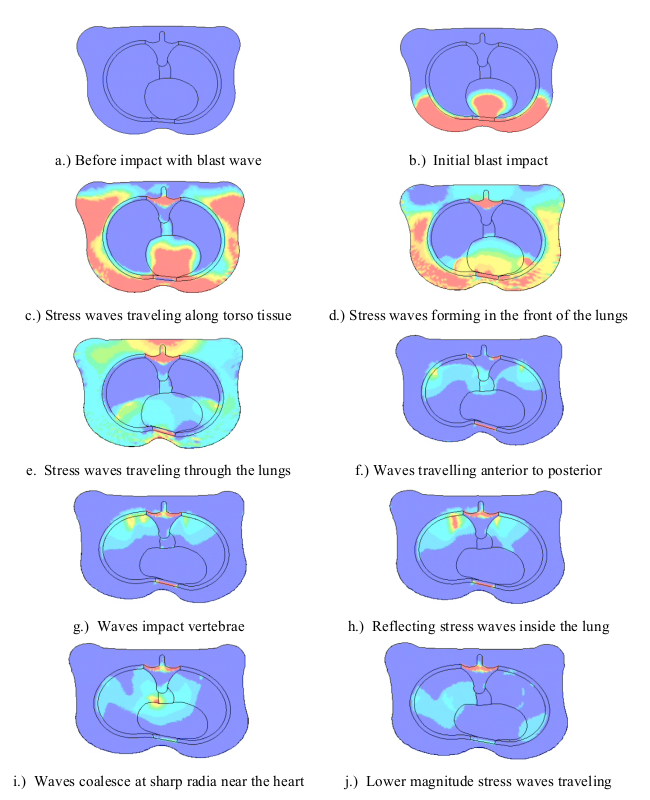
\includegraphics[width=0.95\textwidth]{figures/shockWaveInTorso.png}
    \caption{Finite element analysis done using LS-Dyna to model shock waves traversing a cross-sectional slice of a human torso.  Material models from the LS-Dyna library of available models were used \cite{Josey10}.}
    \label{figShockWaveInLung}
\end{figure}

BABT occurs at the microscopic level of alveoli, which make up the parenchyma, i.e., the spongy tissue of lung that comprises around 90\% of lung by volume, cf.\ Fig.~\ref{figLungDrawing}, there being some 500 million alveoli in a typical human lung.  Most damage occurs just beneath the visceral pleural, as seen in Fig.~\ref{figDamagedLung}, and is thought to be a consequence of the large disparity in wave speeds between solid tissues ($\sim$1,500~m/s) and the spongy parenchyma ($\sim$30-40~m/s) \cite{Stuhmiller08}.  The objective of this work is to develop a mechanistic multi-scale model that is capable of describing the deformation and damage that occur at an alveolar level, caused by a shock wave traveling through the parenchyma, induced through either a blast or a ballistic impact to a soldier's PPE.  In-silico experiments done using this microscopic model are to be used to `inform' our macroscopic model in those areas where actual lung experiments are difficult if not impossible to perform.

\begin{figure}
    \centering
    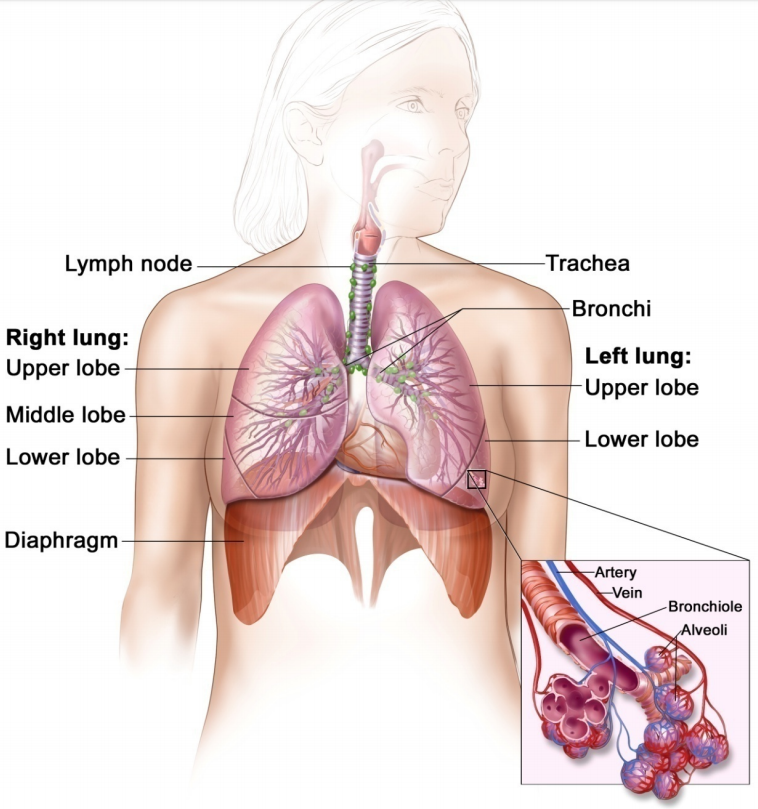
\includegraphics[width=0.7\textwidth]{figures/theRespiratorySystem.png}
    \caption{A medical drawing of the respiratory system \cite{Josey10}.}
    \label{figLungDrawing}
\end{figure}

\begin{figure}
    \centering
    \includegraphics[width=0.7\textwidth]{figures/lungInjuryResultingFromBlast.png}
    \caption{Lungs excised from animals (most likely ovine) who expired from injuries caused by a blast \cite{Stuhmiller08}.}
    \label{figDamagedLung}
\end{figure}

\section{Problem Statement}

Pulmonary contusion is one of the most common thoracic soft-tissue injuries caused by blunt trauma, with a mortality rate of 10-25\% \cite{Stitzeletal05}.  Damage to lungs is the main cause of morbidity following high-level blast exposures \cite{Stuhmilleretal88}.  Lung laceration is also common and debilitating \cite{VlessisTrunkey97}.  Existing constitutive models for lung tissue were developed from limited static test data, e.g., Fung, Vawter \textit{et~al}.\ \cite{Fungetal78,Vawteretal79,Vawter80} These models, and others developed since then, omit relevant physics pertinent to blast and ballistic impacts required to assess BABT.  They also require cumbersome optimization protocols to fit non-unique parameter sets \cite{Gayziketal07,Gayziketal11}, and\slash or are not validated against independent data \cite{Yuenetal08}.  Better lung models suitable for dynamic analysis are needed so that the Army can design improved PPE to better protect their soldiers.

The primary objective of the ARL-WMRD project \textit{Modeling Large Deformations and Stress Wave Mechanics in Soft Biological Tissue\/} is to develop such models for deformation and damage\slash injury assessment.  These are continuum models derived from thermo\-dynamics that utilize internal state variables to account for the irreversible aspects of response \cite{ClaytonFreed19,ClaytonFreed20}.  Models (both macro\-scopic and micro\-scopic) are specifically sought whose parameters are physical and whose parameterization is straightforward.  Characterization of the parameters in a model requires experimental data.  This presents an enormous challenge, one that is being addressed in the ARL-WMRD project through other university collaborators.  

Performing experiments for the purpose of model characterization is extremely difficult when it comes to modeling lung.  Lung is a structure; parenchyma is a material.  Therefore, one would normally choose to test the parenchyma, and from these data extract one's model parameters but, because of its spongy nature, we are challenged to do so in a physically meaningful way.  Consequently, one typically tests whole lungs, or lobes thereof, and from these structural experiments we are tasked to extract material parameters through an inverse analysis.  An alternative approach whereby one could, in principle, acquire parameters for the continuum models being developed at ARL-WMRD would be to homo\-genize a microscopic structural response for the alveoli of parenchyma.  The work presented here addresses this approach in our modeling of deformation, damage and injury in alveolar structures.

Our approach is also advantageous for understanding the influence of microstructure on the higher-scale continuum properties.  Curve fitting to macroscopic data alone does not provide such insight.  This multi-scale approach can also be used to determine properties for regimes (stress\slash strain\slash strain-rate histories) that cannot be reached experimentally, due to limitations in testing facilities, capabilities, or sufficient animal\slash human tissue availability. 

The narrative that follows seeks to develop two material models for lung: one for mechanical deformation and the other for damage\slash injury\slash trauma.  Models are sought whose parameters have physical interpretation.  Ideally, they will enhance our understanding of the deformation and damage mechanisms at play during BABT.  Specifically, they will describe how alveoli respond to pressure-waves and\slash or shear-waves as these wave fronts pass through them.  This modeling will be accomplished by constructing a multi-scale model connecting the parenchyma (macro) and alveolar (micro) levels.  In-silico experiments could then be done on the alveolar structural model, whose homogenized response could serve as an aid in the characterization of ARL's continuum models.  These ARL-WMRD continuum models are being designed to perform efficiently in their implementation in finite element codes.  This will allow for BABT analyses to be done during the design of future PPE with an ultimate goal of saving soldiers lives.

The primary purpose of this work is to provide a micro\-scopic model for lung tissue that can be used as an aid in the parameterization of a macro\-scopic model for lung that will be reasonably accurate yet efficient to run in full torso finite element analyses to study BABT for the purpose of improving PPE.

\section{Approach}

Figure~\ref{figRatLung} shows micrographs from a rat lung taken at different magnifications. In the lower-resolution image one sees numerous alveoli that became exposed because of the sectioning process.  Also present are several alveolar ducts that connect individual alveoli to a bronchial tree.  In the higher-resolution image we observe the faceted structure of these alveoli, wherein one can see the septal chords and membranes, the latter being traversed by capillaries through which gas exchange occurs.  Gas exchange will not be modeled here.

\begin{figure}
    \centering
    \subfigure[Magnification at 100X. This is Fig.~5 in Freed \textit{et~al}.\ \cite{Freedetal12}.]{
        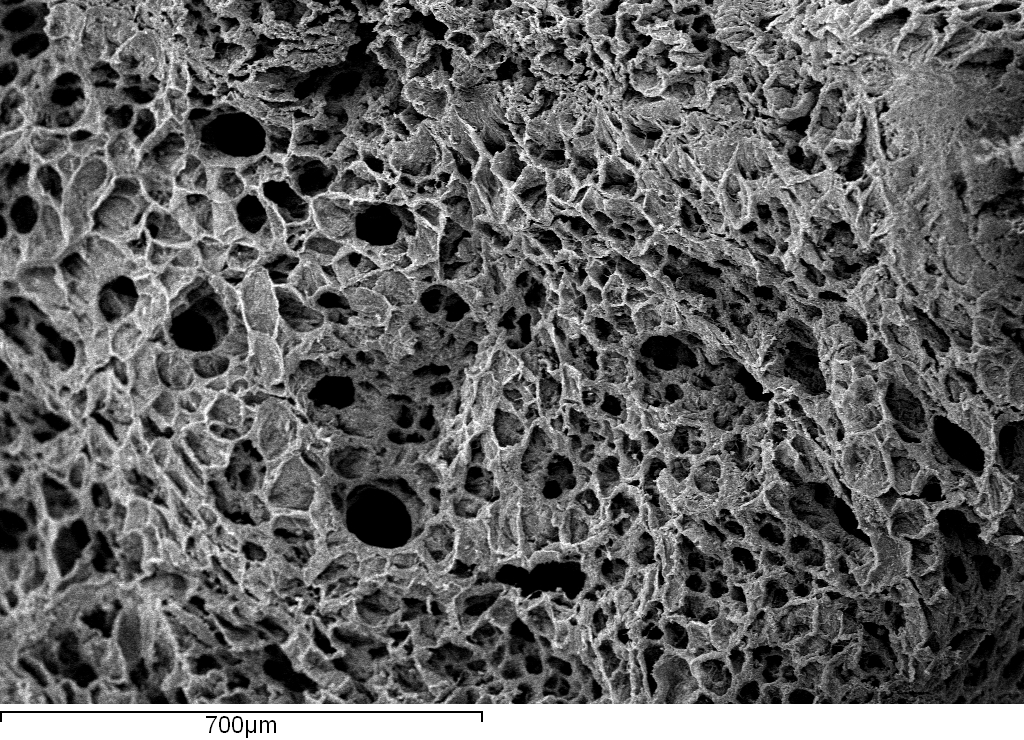
\includegraphics[width=0.45\textwidth]{figures/ratLung100X.jpg}
        \label{figRatLung100}
    }
    \hfill
    \subfigure[Magnification at 750X. This is Fig.~7 in Freed \textit{et~al}.\ \cite{Freedetal12}.]{
        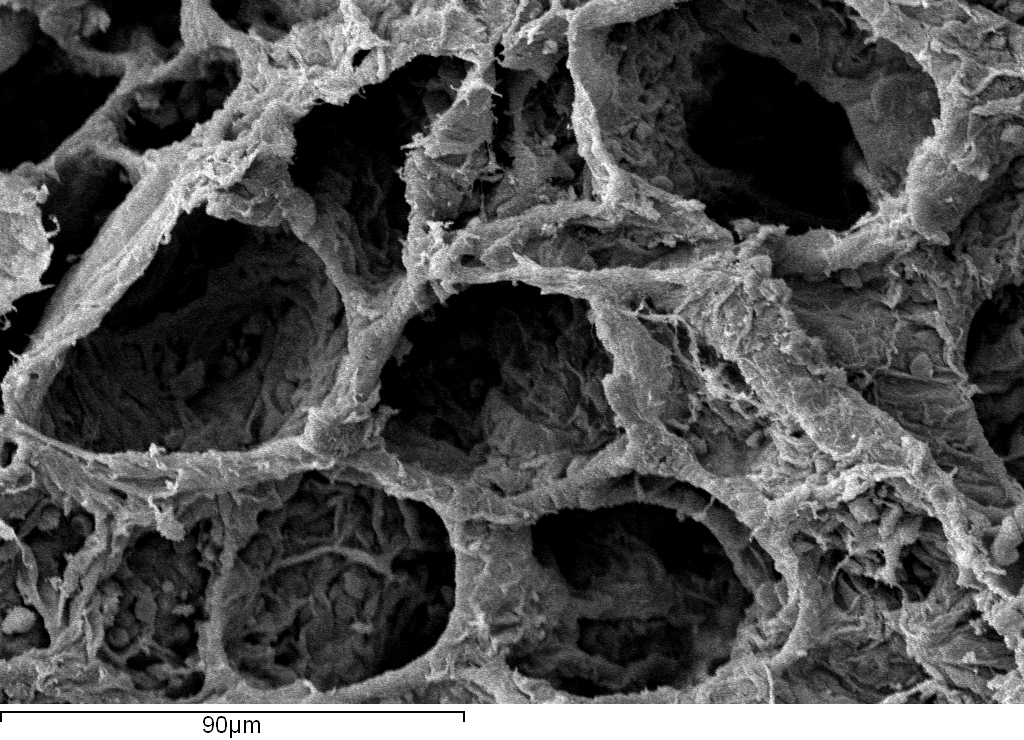
\includegraphics[width=0.45\textwidth]{figures/ratLung750X.jpg}
        \label{figRatLung750}
    }
    \caption{SEM photographs from a sectioned rat lung.  The alveolar diameter in rat lung is about one quarter the alveolar diameter in human lung.}
    \label{figRatLung}
\end{figure}

Alveolar geometry is modeled here as a dodecahedron, i.e., a soccer-ball like structure comprised of twelve pentagonal facets bordered by thirty septal cords that are connected at twenty vertices.  Each vertex links three neighboring cords of the alveolus with a fourth chord from a neighboring alveolus.  BABT can occur through multiple mechanisms, e.g., tearing of septal cords and\slash or alveolar membranes, and in more severe cases, rupturing of capillaries can also happen causing interstitial fluids and blood to leak into neighboring alveoli, all illustrated in Fig.~\ref{figAlveolarDamage}.  Our dodecahedral model for alveoli is capable of capturing these trauma events.

\begin{figure}
    \centering
    \subfigure[Immunohistochemical staining for hemoglobin showing edema fluid buildups (arrows) caused by blast injury.]{
        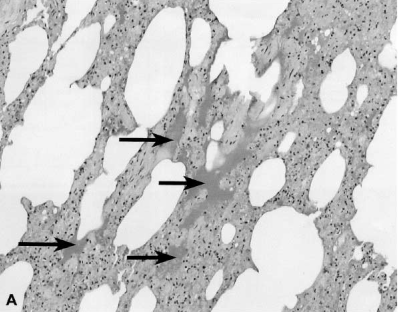
\includegraphics[width=0.3\textwidth]{figures/edemaDamage.png}
        \label{figAlveolarDamageA}
    }
    \hfill
    \subfigure[Histopathology image showing tearing of septal membranes (arrows) caused by blast injury.]{
        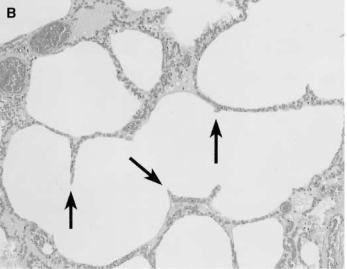
\includegraphics[width=0.3\textwidth]{figures/septalDamage.png}
        \label{figAlveolarDamageB}
    }
    \hfill
    \subfigure[Electron microscope image showing perforations (arrows) of the alveolar wall caused by blast injury.]{
    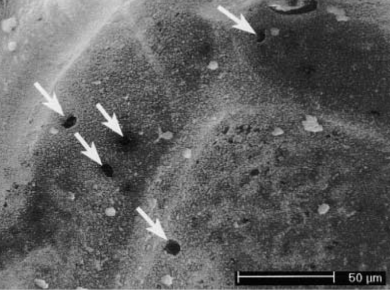
\includegraphics[width=0.3\textwidth]{figures/alveolarDamage.png}
    \label{figAlveolarDamageC}
    }
    \caption{All images were from Tsokos \textit{et~al}.\ \cite{Tsokosetal03}.}
    \label{figAlveolarDamage}
\end{figure}

\begin{conj}
\textit{A micro\-scopic strain field, measured at the scale of alveoli, is the same as its macro\-scopic strain field in which it resides, measured at the scale of parenchyma.  The motion is affine, and the local motion is homogeneous.}  
\label{conjecture}
\end{conj}

This hypothesis was tested and confirmed in an experimental study done by Butler \textit{et~al}.\ \cite{Butleretal96} where they used light scattering to study changes in geometry of the septal planes in alveoli, from which they concluded: ``the micro\-scopic strain field does not differ significantly from the macro\-scopic field.''  We employ this hypothesis by taking the deformation gradient from, say, a Gauss point in a finite element model of lung, e.g., from a Gauss point associated with Fig.~\ref{figShockWaveInLung}, and imposing it as a far-field deformation onto our dodecahedral model of an alveolus.  From this kinematic input we arrive at an upper bound on the macro\-scopic stress\slash stiffness response, akin to a Voigt approximation, through a homogenization of the micro\-scopic forces created within our structural model for an alveolus.

The authors of a recent review article on alveolar strain finished by writing:
\begin{quotation}
    \noindent\small ``In general, computational mechanics approaches to determine function in a healthy or diseased lung have proven to be useful in explaining or measuring observations that are not captured by imaging modalities. However, for these models to fully explain complex physiological mechanical events, appropriate mechanical properties, boundary conditions, and mechanical loads must be identified. Moreover, validation of such computational models, which is an essential component of any computational mechanics approach, remains to be a challenge in the analysis of soft tissue mechanics.''
    
    \nopagebreak
    \mbox{} \hfill Roan \& Waters \cite[pg.~L633]{RoanWaters11} \normalsize
\end{quotation}
In this research we set out to develop a constitutive framework for alveolar mechanics, fully cognizant of the aforementioned challenges.  Our objectives are different from those of prior studies in alveolar mechanics in that we seek to describe the response\slash injury of a human lung that has been subjected to a stress wave propagating across the thorax region caused by an impact from either a blunt object or a blast wave.  Consequently, some important aspects in the modeling of a breathing lung are thought to be less impactful here, e.g., the effect of surfactant in keeping alveoli from collapsing at the end of expiration.

As a foundation, we adopt the guideline:
\begin{quotation}
	\noindent\small ``Constitutive equations are phenomenological. They are regarded as empirical by experimenters, and axiomatic by mathematicians.  In biomechanics, we often try to derive them on the basis of micro\-structure $\ldots$ in order to gain a better understanding, or to get some guidance to the mathematical form.''
	
	\nopagebreak
	\mbox{} \hfill Y.-C.~Fung \cite[pg.~431]{Fung90} \normalsize
\end{quotation}
The approach adopted here is to use the geometry of a dodecahedron as a \textit{micro}\-scopic mechanical model for alveoli, whose far-field response to mechanical stimuli, in accordance with our Conjecture on pg.~\pageref{conjecture}, will be used to inform the development of a \textit{macro\/}scopic mechanical model for parenchyma, \cite{ClaytonFreed19,ClaytonFreed20} the predominant tissue in lung.  This is deemed necessary because of the complex porous structure of parenchyma, as compared with the homo\-geneous structure of rubbery elastic solids whose theories have historically been employed to model parenchyma \cite{Fung75,Fungetal78,Vawteretal79,Fung88}.  The ARL-WMRD continuum (macroscopic) model for parenchyma \cite{ClaytonFreed19} will be implemented into finite element codes by others on our team with an end objective of providing a numerical tool that can be used by Army engineers in their efforts to develop improved and more effective designs for a soldier's PPE. 

\section{Organization}

This document is organized in the following manner.  Part~\ref{partDodecahedron} introduces the dodecahedron as a model for alveoli.  Its geometric properties are derived in detail with regards to its three geometric features: 1D septal chords, 2D septal membranes, and 3D volume.  Part~\ref{partKinematics} develops the kinematics required for us to model a deforming dodecahedron, again focusing on the 1D~chords, 2D~membranes, and the 3D~volume within, including the shape functions needed for interpolating each geometry.  Part~\ref{partConstitutive} derives constitutive models suitable for describing the thermo-mechanical response for the structural constituents of an alveolus: its septal chords, its permeable membranes, and its volume.  Part~\ref{partNumericalMethods} presents numerical methods used for solving first- and second-order, ordinary, differential equations (ODEs), and for solving spatial integrations along a bar, across a pentagon, and throughout a tetrahedron using Gaussian quadrature schemes designed for each geometry.  Part~\ref{partVariational} describes a variational formulation used to create our structural modeling of an alveolus, which consists of three separate models: one comprised of septal chords, another comprised of septal membranes, and the third comprised of alveolar volume.  All interpolate their stresses to the vertices where the forces from each are summed and homogenized for return to the macroscopic solver.  Constitutive equations suitable for modeling biological tissues are derived from thermo\-dynamics using the theory of implicit elasticity presented in Appendix~\ref{appImplicitElasticity}.


%\setcounter{equation}{0}
%\setcounter{figure}{0}
%\setcounter{section}{0}
%\setcounter{table}{0}
\part{Dodecahedra: A Model for Alveoli}
\label{partDodecahedron}

Typical alveoli are fourteen sided polyhedra with one face normally being open as a mouth to an alveolar duct, and whose septal membranes typically become flat at trans\-pulmonary pressures as low as 2~cm~$\text{H}_2\text{O}$ \cite{HoppinHildebrandt77}.  To capture the micro\-structural features of lung, researchers have modeled both alveoli and alveolar ducts, as seen in Fig.~\ref{figRatLung}; we only address alveoli here.  One of three different geometric shapes is usually employed when modeling an alveolus: a dodecahedron introduced by Frankus \& Lee \cite{FrankusLee74} in 1974, a rhombic dodecahedron introduced by de~Ryk, Thiesse, Namati \& McLennan \cite{Ryketal07} in 2007, and a truncated octahedron, i.e., a tetrakaidecahedron, introduced by Dale, Matthews \& Schroter \cite{Daleetal80} in 1980.  The dodecahedron and rhombic dodecahedron are both twelve sided polyhedra with faces being pentagons and rhombuses, respectively.  A tetrakaidecahedron is a pair of pyramids stacked bottom to bottom, forming an octahedron, whose six points are then removed.  The end result is a fourteen sided polyhedron with six faces that are squares and eight faces that are hexagons, where like shapes have like dimensions.

The tetrakaidecahedron and rhombic dodecahedron are both volume filling.  This property is preferred whenever one sets out to construct assemblages of alveoli to build a micro\-structural model that is to be solved numerically via a finite element method.  The purpose of such an exercise is to homogenize the response of an alveolar assembly up to the macroscopic level, i.e., the level of a continuum mass point, a.k.a., the parenchyma \cite{Daleetal80,DennySchroter95,DennySchroter97,DennySchroter00,Koweetal86,Ryketal07,Chenetal14}.  Such a finite element model can serve as a representative volume element (RVE) for parenchyma.

The dodecahedron is an isotropic structure, or very nearly so as we shall show, and is nearly volume filling \cite{Kimmeletal87}.  A dodecahedron is one of the five perfectly symmetric solids in geometry.  It becomes a preferred geometry whenever a single alveolus is to be used as the RVE of homo\-genization, and from which closed form solutions have been derived \cite{BudianskyKimmel87,KimmelBudiansky90,Kimmeletal87,Freedetal12}.  Here isotropy of the microstructure ensures an isotropic macro response.  Parenchyma, as a tissue, is isotropic \cite{Weedetal15,Fung88,Hughesetal72}; whereas, lung, as an organ, is a complex, heterogeneous structure \cite{Mead73,West07}.  This distinction has, from time-to-time, been forgotten \cite{DennySchroter06}.  

For the reasons stated above, a dodecahedron, with vertices labeled according to Fig.~\ref{figDodecahedronB}, is the geometric structure selected for use in this study. The question of how one assigns a co-ordinate system to a dodecahedron is discussed first.  Given this co-ordinate system, vertices of a dodecahedron are then assigned from which its septal chords and septal membranes are readily established.

\begin{figure}
    \centering
    \subfigure[A cube is contained within a dodecahedron, with one of its five possible orientations being displayed.  Atop each face of the cube resides four pentagonal sub-areas that form the shape of a hipped roof line.]{
        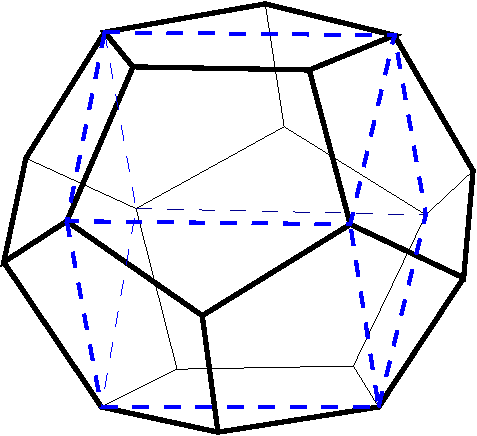
\includegraphics[width=0.45\textwidth]{figures/dodecahedron.png}
        \label{figDodecahedronA}
    }
    \hfill
    \subfigure[ Vertices 1 through 8 are located at the corners of such a cube.  The centroid for the cube is also the centroid for the dodecahedron.  Vertices 9 through 20 are corners of the hipped roof lines residing above each face of the cube.]{
        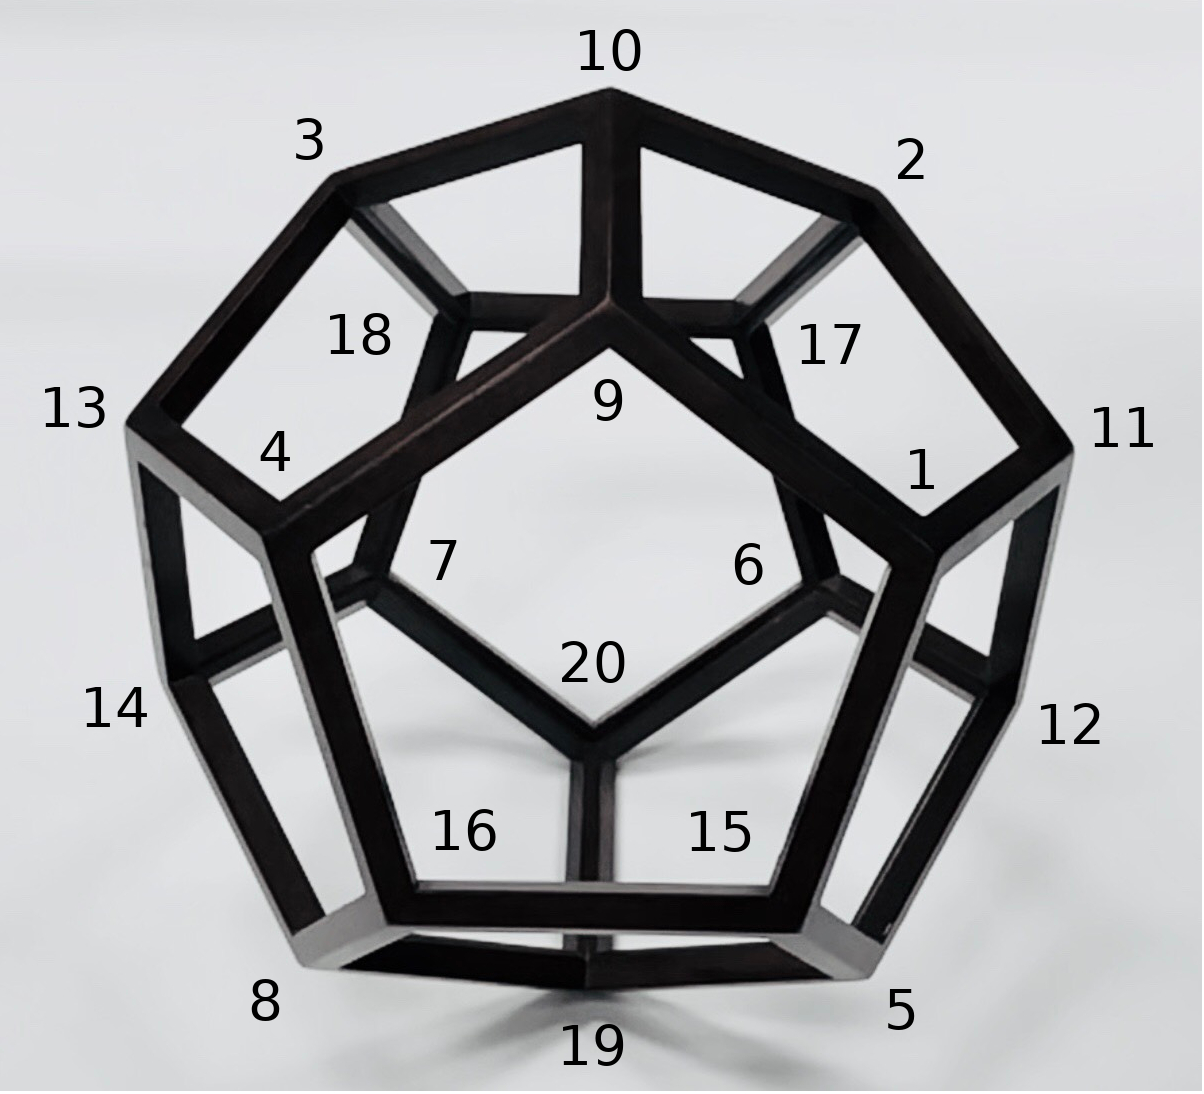
\includegraphics[width=0.45\textwidth]{figures/dodecahedronVertices.jpg}
        \label{figDodecahedronB}
    }
	\caption{Geometric representations for a dodecahedron.}
	\label{figDodecahedron}
\end{figure}

\section{Co-ordinate Indexing}
\label{reindexing3D}

An orthonormal set of base vectors $( \vec{\boldsymbol{\imath}} , \vec{\boldsymbol{\jmath}} , \vec{\boldsymbol{k}} )$ is assigned to a dodecahedron whose origin resides at its centroid and whose directions align with a set of far-field base vectors used for reference in one's finite element model of a lung.  The question is: How does one orient the indexing scheme of Fig.~\ref{figDodecahedron} against this basis?  Alternatively:  How can one describe a mapping $( \vec{\boldsymbol{\imath}} , \vec{\boldsymbol{\jmath}} , \vec{\boldsymbol{k}} ) \overset{\text{?}}{\mapsto} ( \vec{\mathbfsf{E}}_1 , \vec{\mathbfsf{E}}_2 , \vec{\mathbfsf{E}}_3 )$ wherein an ortho\-normal set of base vectors $( \vec{\mathbfsf{E}}_1 , \vec{\mathbfsf{E}}_2 , \vec{\mathbfsf{E}}_3 )$ is to serve as the reference basis for our alveolar dodecahedron to which the indexing scheme presented in Fig.~\ref{figDodecahedron} applies?

Given that a finite element model for lung exists, then a deformation gradient $\mathbfsf{F}$ can be made available at any mass point therein whereat an alveolus of interest resides.  Let the components of this deformation gradient be $F_{ij}$, $i, j = 1,2,3$, when evaluated in the co-ordinate frame $( \vec{\boldsymbol{\imath}} , \vec{\boldsymbol{\jmath}} , \vec{\boldsymbol{k}} )$, which is the co-ordinate frame of the finite element analysis.  A Gram-Schmidt (or \textbf{QR}) decomposition of a non-singular $3 \! \times \! 3$ matrix results in a tangent vector $\vec{\mathbfsf{g}}_1$ and normal vector $\vec{\mathbfsf{g}}_1 \times \vec{\mathbfsf{g}}_2$ that remain invariant under transformations of the triangular matrix \textbf{R} \cite{McLellan80}.  These convected base vectors $( \vec{\mathbfsf{g}}_1 , \vec{\mathbfsf{g}}_2 , \vec{\mathbfsf{g}}_3 )$ rotate out of basis $( \vec{\mathbfsf{E}}_1 , \vec{\mathbfsf{E}}_2 , \vec{\mathbfsf{E}}_3 )$ via a Gram rotation \cite{FreedZamani18}.  Given this geometric information, Paul, Freed \& Clayton \cite{Pauletal20} were able to provide an answer to the above question of co-ordinate frame selection.

Their approach begins by establishing the extent of transverse shear crossing each of the co-ordinate directions $( \vec{\boldsymbol{\imath}} , \vec{\boldsymbol{\jmath}} , \vec{\boldsymbol{k}} )$, as quantified by
\begin{equation}
\mathcal{G}_1 =\dfrac{\sqrt{F^{\,2}_{21}+F^{\,2}_{31}}}{F_{11}} , \quad
\mathcal{G}_2 =\dfrac{\sqrt{F^{\,2}_{12}+F^{\,2}_{32}}}{F_{22}} , \quad
\mathcal{G}_3 =\dfrac{\sqrt{F^{\,2}_{13}+F^{\,2}_{23}}}{F_{33}}
\end{equation} 
where $\mathcal{G}_i$ is a measure of the shear deformation cutting across the $i^{\text{th}}$ direction.  Unit vector $\vec{\mathbfsf{E}}_1$ is selected as that direction from the set $\{ \vec{\boldsymbol{\imath}} , \vec{\boldsymbol{\jmath}} , \vec{\boldsymbol{k}} \}$ which possesses minimal transverse shear.  Once selected, there are two possible planes that contain base vector $\vec{\mathbfsf{E}}_1$, and the one selected whose normal is to be $\vec{\mathbfsf{E}}_1 \times \vec{\mathbfsf{E}}_2$ is that plane with the least amount of in-plane shear, which can be determined by taking appropriate dot products between column vectors $\boldsymbol{f}_i = \{ F_{1i} \; F_{2i} \; F_{3i} \}^{\mathsf{T}}$, $i=1,2,3$.  Vector $\boldsymbol{f}_i$ has elements taken from the $i^{\text{th}}$ column of matrix $F_{ji}$, which represents the deformation gradient $\mathbfsf{F}$ evaluated in $( \vec{\boldsymbol{\imath}} , \vec{\boldsymbol{\jmath}} , \vec{\boldsymbol{k}} )$.  Their strategy is summarized in Alg.~\ref{alg:pivoting}.

Algorithm \ref{alg:pivoting} inputs a deformation gradient $\mathbfsf{F}$ whose components $F_{ij}$ are evaluated in the co-ordinate system $(  \vec{\boldsymbol{\imath}} , \vec{\boldsymbol{\jmath}} , \vec{\boldsymbol{k}} )$ associated with, in our case, a finite element model for lung.  The algorithm outputs an orthogonal matrix $\mathbfsf{P}$ that re-indexes the components of deformation gradient $F_{ij}$ into an equivalent form where $\mathbfsf{F} = \mathcal{F}_{ij} \, \vec{\mathbfsf{E}}_i \otimes \vec{\mathbfsf{E}}_j$.  It is this re-indexed matrix $\mathcal{F}_{ij}$ that is to be subjected to Gram-Schmidt factorization, which is discussed later in Part~\ref{partKinematics}.  

\begin{algorithm}
    \KwIn{Deformation gradient $\mathbfsf{F}$ with components $F_{ij}$ expressed in $( \vec{\boldsymbol{\imath}} , \vec{\boldsymbol{\jmath}} , \vec{\boldsymbol{k}} )$.}
    \uIf{$\mathcal{G}_1 \le \mathcal{G}_2 \: \mathbf{and} \; \mathcal{G}_1 \le \mathcal{G}_3$}
    {\eIf{$\boldsymbol{f}_1 \cdot \boldsymbol{f}_2 \le \boldsymbol{f}_1 \cdot \boldsymbol{f}_3$}{$[ \boldsymbol{\mathcal{F}}_1 ] = [ \mathbfsf{P}_1 ]^{\mathsf{T}} [ \mathbfsf{F} ] [ \mathbfsf{P}_1 ] : \; [ \boldsymbol{\mathcal{F}} ] = [ \boldsymbol{\mathcal{F}}_1 ] , \; [ \mathbfsf{P} ] = [ \mathbfsf{P}_1 ],$ \\ $\phantom{[ \boldsymbol{\mathcal{F}}_1 ]} \therefore \; ( \vec{\boldsymbol{\imath}}, \vec{\boldsymbol{\jmath}}, \vec{\boldsymbol{k}} ) \mapsto ( \vec{\mathbfsf{E}}_1, \vec{\mathbfsf{E}}_2, \vec{\mathbfsf{E}}_3 )$}{$[ \boldsymbol{\mathcal{F}}_2 ] = [ \mathbfsf{P}_2 ]^{\mathsf{T}} [ \mathbfsf{F} ] [ \mathbfsf{P}_2 ] : \; [ \boldsymbol{\mathcal{F}} ] = [ \boldsymbol{\mathcal{F}}_2 ] , \; [ \mathbfsf{P} ] = [ \mathbfsf{P}_2 ],$ \\ $\phantom{[ \boldsymbol{\mathcal{F}}_1 ]} \therefore \; ( \vec{\boldsymbol{\imath}}, \vec{\boldsymbol{\jmath}}, \vec{\boldsymbol{k}} ) \mapsto ( \vec{\mathbfsf{E}}_1, \vec{\mathbfsf{E}}_3, \vec{\mathbfsf{E}}_2 )$}}
    \uElseIf{$\mathcal{G}_2 \le \mathcal{G}_1 \: \mathbf{and} \; \mathcal{G}_2 \le \mathcal{G}_3$}
    {\eIf{$\boldsymbol{f}_1 \cdot \boldsymbol{f}_2 \le \boldsymbol{f}_2 \cdot \boldsymbol{f}_3$}{$[ \boldsymbol{\mathcal{F}}_3 ] = [ \mathbfsf{P}_3 ]^{\mathsf{T}} [ \mathbfsf{F} ] [ \mathbfsf{P}_3 ] : \; [ \boldsymbol{\mathcal{F}} ] = [ \boldsymbol{\mathcal{F}}_3 ] , \; [ \mathbfsf{P} ] = [ \mathbfsf{P}_3 ] ,$ \\ $\phantom{[ \boldsymbol{\mathcal{F}}_1 ]} \therefore \; ( \vec{\boldsymbol{\imath}}, \vec{\boldsymbol{\jmath}}, \vec{\boldsymbol{k}} ) \mapsto ( \vec{\mathbfsf{E}}_2, \vec{\mathbfsf{E}}_1, \vec{\mathbfsf{E}}_3 )$}{$[ \boldsymbol{\mathcal{F}}_4 ] = [ \mathbfsf{P}_4 ]^{\mathsf{T}} [ \mathbfsf{F} ] [ \mathbfsf{P}_4 ] : \; [ \boldsymbol{\mathcal{F}} ] = [ \boldsymbol{\mathcal{F}}_4 ] , \; [ \mathbfsf{P} ] = [ \mathbfsf{P}_4 ] ,$ \\ $\phantom{[ \boldsymbol{\mathcal{F}}_1 ]} \therefore \; ( \vec{\boldsymbol{\imath}}, \vec{\boldsymbol{\jmath}}, \vec{\boldsymbol{k}} ) \mapsto ( \vec{\mathbfsf{E}}_2, \vec{\mathbfsf{E}}_3, \vec{\mathbfsf{E}}_1 )$}}
    \Else{
        {\eIf{$\boldsymbol{f}_1 \cdot \boldsymbol{f}_3 \le \boldsymbol{f}_2 \cdot \boldsymbol{f}_3$}{$[ \boldsymbol{\mathcal{F}}_5 ] = [ \mathbfsf{P}_5 ]^{\mathsf{T}} [ \mathbfsf{F} ] [ \mathbfsf{P}_5 ] : \; [ \boldsymbol{\mathcal{F}} ] = [ \boldsymbol{\mathcal{F}}_5 ] , \; [ \mathbfsf{P} ] = [ \mathbfsf{P}_5 ] ,$ \\ $\phantom{[ \boldsymbol{\mathcal{F}}_1 ]} \therefore \; ( \vec{\boldsymbol{\imath}}, \vec{\boldsymbol{\jmath}}, \vec{\boldsymbol{k}} ) \mapsto ( \vec{\mathbfsf{E}}_3, \vec{\mathbfsf{E}}_1, \vec{\mathbfsf{E}}_2 )$}{$[ \boldsymbol{\mathcal{F}}_6 ] = [ \mathbfsf{P}_6 ]^{\mathsf{T}} [ \mathbfsf{F} ] [ \mathbfsf{P}_6 ] : \; [ \boldsymbol{\mathcal{F}} ] = [ \boldsymbol{\mathcal{F}}_6 ] , \; [ \mathbfsf{P} ] = [ \mathbfsf{P}_6 ] ,$ \\ $\phantom{[ \boldsymbol{\mathcal{F}}_1 ]} \therefore \; ( \vec{\boldsymbol{\imath}}, \vec{\boldsymbol{\jmath}}, \vec{\boldsymbol{k}} ) \mapsto ( \vec{\mathbfsf{E}}_3, \vec{\mathbfsf{E}}_2, \vec{\mathbfsf{E}}_1 )$}}}
    \KwOut{Deformation gradient $\mathbfsf{F}$ with components $\mathcal{F}_{ij}$ expressed in $( \vec{\mathbfsf{E}}_1 , \vec{\mathbfsf{E}}_2 , \vec{\mathbfsf{E}}_3 )$, as re-indexed by the orthogonal matrix $[ \mathbfsf{P} ]$.}
    \caption{Pivoting of the co-ordinate system.}
    \label{alg:pivoting}
\end{algorithm}

There are six cases that can arise.  Their associated orthogonal matrices are
\begin{subequations}
    \small
    \begin{align}
    [ \mathbf{P}_1 ] & = \begin{bmatrix}
    1 & 0 & 0\\
    0 & 1 & 0\\
    0 & 0 & 1
    \end{bmatrix} & 
    [ \mathbf{P}_2 ] & = \begin{bmatrix}
    1 & 0 & 0\\
    0 & 0 & 1\\
    0 & 1 & 0
    \end{bmatrix} &
    [ \mathbf{P}_3 ] & = \begin{bmatrix}
    0 & 1 & 0\\
    1 & 0 & 0\\
    0 & 0 & 1
    \end{bmatrix} \notag \\
    [ \mathbf{P}_4 ] & = 
    \begin{bmatrix}
    0 & 0 & 1\\
    1 & 0 & 0\\
    0 & 1 & 0
    \end{bmatrix} & 
    [ \mathbf{P}_5 ] & = \begin{bmatrix}
    0 & 1 & 0\\
    0 & 0 & 1\\
    1 & 0 & 0
    \end{bmatrix} &
    [ \mathbf{P}_6 ] & = \begin{bmatrix}
    0 & 0 & 1\\
    0 & 1 & 0\\
    1 & 0 & 0
    \end{bmatrix} \\ 
    \intertext{\normalsize whose affiliated components for the re-indexed deformation gradient are}
    [ \boldsymbol{\mathcal{F}}_1 ] & = \begin{bmatrix}
    F_{11} & F_{12} & F_{13}\\
    F_{21} & F_{22} & F_{23}\\
    F_{31} & F_{32} & F_{33}
    \end{bmatrix} & 
    [ \boldsymbol{\mathcal{F}}_2 ] & = \begin{bmatrix}
    F_{11} & F_{13} & F_{12}\\
    F_{31} & F_{33} & F_{32}\\
    F_{21} & F_{23} & F_{22}
    \end{bmatrix} &
    [ \boldsymbol{\mathcal{F}}_3 ] & = \begin{bmatrix}
    F_{22} & F_{21} & F_{23}\\
    F_{12} & F_{11} & F_{13}\\
    F_{32} & F_{31} & F_{33}
    \end{bmatrix} \notag \\
    [ \boldsymbol{\mathcal{F}}_4 ] & = \begin{bmatrix}
    F_{22} & F_{23} & F_{21}\\
    F_{32} & F_{33} & F_{31}\\
    F_{12} & F_{13} & F_{11}
    \end{bmatrix} &
    [ \boldsymbol{\mathcal{F}}_5 ] & = \begin{bmatrix}
    F_{33} & F_{31} & F_{32}\\
    F_{13} & F_{11} & F_{12}\\
    F_{23} & F_{21} & F_{22}
    \end{bmatrix} & 
    [ \boldsymbol{\mathcal{F}}_6 ] & = \begin{bmatrix}
    F_{33} & F_{32} & F_{31}\\
    F_{23} & F_{22} & F_{21}\\
    F_{13} & F_{12} & F_{11}
    \end{bmatrix}
    \end{align}
    \normalsize
\end{subequations}
where case 1 is the default case whose operator $\mathbfsf{P}_1$ is the identity tensor.

All vectors $\mathbfsf{V}$ with components $\mathcal{V}_i$ evaluated in $( \vec{\mathbfsf{E}}_1 , \vec{\mathbfsf{E}}_2 , \vec{\mathbfsf{E}}_3 )$ will rotate into $( \vec{\boldsymbol{\imath}} , \vec{\boldsymbol{\jmath}} , \vec{\boldsymbol{k}} )$ with components $V_i$ according to the map
\begin{subequations}
    \begin{align}
    V_i & = P_{ij} \mathcal{V}_j & \text{or inversely} & &
    \mathcal{V}_i & = P_{ji} V_j \\
    \intertext{while all tensors $\mathbfsf{T}$ with components $\mathcal{T}_{ij}$ evaluated in $( \vec{\mathbfsf{E}}_1 , \vec{\mathbfsf{E}}_2 , \vec{\mathbfsf{E}}_3 )$ will rotate into $( \vec{\boldsymbol{\imath}} , \vec{\boldsymbol{\jmath}} , \vec{\boldsymbol{k}} )$ with components $T_{ij}$ according to the map}
    T_{ij} & = P_{ik} \mathcal{T}_{k\ell} P_{j\ell} & \text{or inversely} & &
    \mathcal{T}_{ij} & = P_{ki} T_{k\ell} P_{\ell j}
    \end{align}
\end{subequations}
where the latter appears in Alg.~\ref{alg:pivoting} with regards to components of the deformation gradient.

From this point onward, it is assumed that base vectors $( \vec{\mathbfsf{E}}_1 , \vec{\mathbfsf{E}}_2 , \vec{\mathbfsf{E}}_3 )$ are known, and that they serve as the reference basis for our alveolar analysis.

\section{Geometric Properties of a Regular Pentagon}
\label{sec:pentagonGeometry}

Figure~\ref{figRegPentagon} presents a regular pentagon drawn in its natural co-ordinate system with co-ordinates designated as $(\xi, \eta)$.  Vertices of such a pentagon are placed at
\begin{equation}
	\xi = \cos \left( \frac{2(k-1)\pi}{5} + \frac{\pi}{2} \right) \quad
	\eta = \sin \left( \frac{2(k-1)\pi}{5} + \frac{\pi}{2} \right) \quad
	k = 1, 2, \ldots, 5
	\label{regPentagon}
\end{equation}
wherein $k$ denotes the vertex number, as assigned in Fig.~\ref{figRegPentagon}.  These vertices inscribe a pentagon within the unit circle.

\begin{figure}
	\centering
	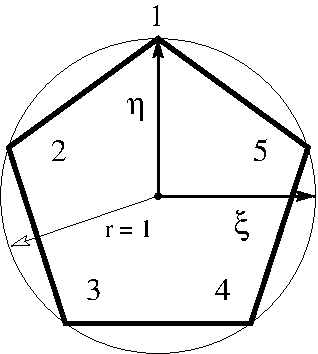
\includegraphics[width=6cm]{figures/regPentagon.png}
	\caption{A regular pentagon inscribed within the unit circle establishes its natural co-ordinate system with co-ordinates $(\xi, \eta)$ described in Eqn.~(\ref{regPentagon}), and whose origin is located at its centroid.  Vertices are numbered counter\-clockwise with the uppermost vertex being labeled~1.}
	\label{figRegPentagon}
\end{figure}

Lengths of the five chords in a regular pentagon, when measured in its natural co-ordinate system, are all
\begin{equation}
	L^p = 2 \cos (\omega) \approx 1.176 
	\label{regPentagonLength}
\end{equation}
while the area of this pentagon is
\begin{equation}
	A^p = \tfrac{5}{4} \tan ( \omega ) \, (L^p)^2 = 
	5 \sin (\omega) \cos (\omega) \approx 2.378
	\label{regPentagonArea}
\end{equation}
where area of the unit circle that inscribes this pentagon is $\pi r^2 \approx 3.142$, $r=1$.  The inside angles of a regular pentagon all measure $2\omega = 108^{\circ}$.  All approximations are truncated at four significant figures.

\section{Geometric Properties of a Regular Dodecahedron}

Like the pentagon considered above, which inscribes the unit circle, here we consider a dodecahedron that inscribes the unit sphere.  Let this geometry be described in its natural co-ordinate system with co-ordinates $(\xi , \eta , \zeta )$ whose origin is located at its centroid, the center of the sphere.  The twenty vertices of this dodecahedron, all of which touch the unit sphere, are placed at
\begin{equation}
\begin{tabular}{ccc}
	$\xi$ & $\eta$ & $\zeta$ \\ \hline
	$\pm 1 / \sqrt{3}$ & $\pm 1 / \sqrt{3}$ & $\pm 1 / \sqrt{3}^{\vphantom{|}}$ \\
	$\pm \phi / \sqrt{3}$ & $\pm 1 / \sqrt{3} \phi$ & 0 \\
	0 & $\pm \phi / \sqrt{3}$ & $\pm 1 / \sqrt{3} \phi$ \\
	$\pm 1 / \sqrt{3} \phi$ & 0 & $\pm \phi / \sqrt{3}$
\end{tabular}
\label{regDodecahedron}
\end{equation}
where $\phi = (1 + \sqrt{5})/2 \approx 1.618$, which is also known as the golden ratio.

Lengths of the thirty chords in a regular dodecahedron, when measured in its natural co-ordinate system, are all
\begin{equation}
	L^d = \frac{2}{\sqrt{3} \phi} \approx 0.7136
	\label{regDodecahedronLength}
\end{equation}
while the volume of such a dodecahedron is
\begin{equation}
	V^d = \frac{40}{3 \sqrt{3} \phi^3} \tan^2 ( \omega ) \sin ( \omega ) \approx 2.785
\label{regDodecahedronVolume}
\end{equation}
where volume of the unit sphere that inscribes the dodecahedron is $\tfrac{4}{3} \pi r^3 \approx 4.189$, $r=1$.

The scale factor to map between the natural co-ordinates of a pentagon, defined in Eq.~(\ref{regPentagon}), with those of a dodecahedron, defined in Eq.~(\ref{regDodecahedron}), is
\begin{equation}
	\frac{L^p}{R^p} = \frac{L^d}{R^p_d} 
	\quad \text{or} \quad
	R^p_d = \frac{R^p L^d}{L^p} = \frac{L^d}{L^p} = 
	\frac{1}{\sqrt{3} \phi \cos (\omega)} \approx 0.6071
	\label{scaleFactor}
\end{equation}
because $R^p = 1$, with scale factor $R^p_d$ being the radius that inscribes a pentagon on the surface of a dodecaheron that itself inscribes an unit sphere.

\section{Dimensions of Human Alveoli}
\label{alveolarSize}

Septal chord length $L(D)$, expressed as a function of alveolar diameter $D$, can be estimated by considering the areal projection of a dodecahedron onto a plane that contains one of its pentagonal faces, which leads to
\begin{equation}
	L = \frac{D}{\tan ( \omega ) ( 1 + \cos ( \alpha ) )} 
	\approx  \frac{D}{2.685} ,
\label{dodecahedralHeight}
\end{equation} 
where $\alpha = \textfrac{\pi}{10} = 18^{\circ}$.  (There are twenty, equal, pie-shaped wedges that comprise this projected area.)  This is an average of the shortest and longest distances across this plane of projection.  Alveolar diameter $D$ is a property that can be measured in histological studies of parenchyma.  

To dimension the alveoli of human lung, Sobin, Fung \& Tremer \cite{Sobinetal88} measured the mean diameter across an individual alveolus, viz., $D$ of Eq.~(\ref{dodecahedralHeight}),  sectioned from human lungs that were fixed at three different pressures.  Samples were taken from nine lungs extracted postmortem from individuals between 16 to 89 years of age.\footnote{%
	Sobin \textit{et~al}.\ \cite{Sobinetal88} also documented an age effect in these data that has been averaged over here, i.e., ignored.
}
At a transpulmonary pressure of 4~cm~$\text{H}_2$O, the mean alveolar diameter was $D = 191$ $\pm$ 86~$\mu$m determined from a sampling size of 1423; at a pressure of 10~cm~$\text{H}_2$O, $D = 202$ $\pm$ 88~$\mu$m determined from a sampling size of 1296; and at a pressure of 14~cm~$\text{H}_2$O, $D = 235$ $\pm$ 99~$\mu$m determined from a sampling size of 1083.  These data are plotted in Fig.~\ref{septalLengthFig}.  All reported and drawn error bounds pertain to plus\slash minus one standard deviation in error.

\begin{figure}
	\centering
    \subfigure[Mean and standard deviations for alveolar diameters in human lung.   
        \cite{Sobinetal88}]{
        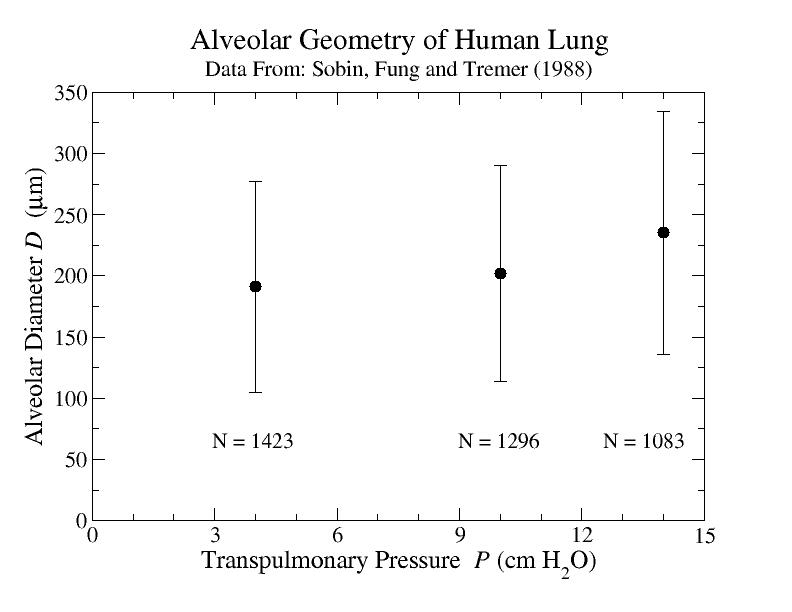
\includegraphics[width=0.45\textwidth]{figures/septalLength.jpg}
        \label{figSeptalLengthA}
    }
    \hfill
    \subfigure[A typical histogram for these statistics, truncated at alveolar diameters below 24~$\mu$m.]{
        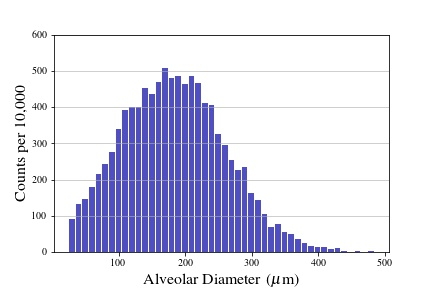
\includegraphics[width=0.5\textwidth]{figures/alveolarDiaHistogram.jpg}
        \label{figSeptalLengthB}
    }
	\caption{Alveolar diameters in human lung.}
	\label{septalLengthFig}
\end{figure}

\section{Geometric Properties for Irregular Pentagons and Dodecahedra}
\label{sec:geometries}

Formul\ae\ (\ref{regPentagonArea} \& \ref{regDodecahedronVolume}) only apply for regular pentagons and dodecahedra evaluated in their respective natural co-ordinate systems.  For irregular dodecahedra, the areas of its irregular pentagons are calculated via\footnote{
	Bourke, P., ``Polygons, Meshes.'' \texttt{http://paulbourke.net/geometry}.
}
\begin{equation}
	A = \frac{1}{2} \sum_{i=1}^5 ( x_i y_{i+1} - x_{i+1} y_i)
	\label{irregularPentagonArea}
\end{equation}
where $x_6 \Leftarrow x_1$ and $y_6 \Leftarrow y_1$.  In order for the predicted area to be positive when using this formula, it is necessary that the vertices $(x_i , y_i)$ index counterclockwise, as drawn in Fig.~\ref{figRegPentagon}.  The centroid of this pentagon has co-ordinates\footnotemark[\value{footnote}]
\begin{subequations}
	\label{centroidPentagon}
	\begin{align}
		c_x & = \frac{1}{6 A} \sum_{i=1}^5 (x_i + x_{i+1})
			( x_i y_{i+1} - x_{i+1} y_i) \\
		c_y & = \frac{1}{6 A} \sum_{i=1}^5 (y_i + y_{i+1})
		( x_i y_{i+1} - x_{i+1} y_i)
	\end{align}
\end{subequations}
wherein the vertex co-ordinates $x_i$ and $y_i$ are quantified in a 2D pentagonal frame of reference, e.g., as established later in Fig.~\ref{figPentagonCoord}.

To compute the volume of an irregular dodecahedron, use the formula\footnote{
	Colins, K.~D., ``Cayley-Menger Determinant.'' From MathWorld--A Wolfram Web Resource, created by Eric W.\ Weisstein. \texttt{http://mathworld.wolfram.com/Cayley\-MengerDeterminant.html}.
}
\begin{equation}
	288 \, V^{\,2}_{tet} = \left| \begin{matrix}
	0 & 1 & 1 & 1 & 1 \\
	1 & 0 & \ell_{12}^{\,2} & \ell_{13}^{\,2} & \ell_{14}^{\,2} \\
	1 & \ell_{21}^{\,2} & 0 & \ell_{23}^{\,2} & \ell_{24}^{\,2} \\
	1 & \ell_{31}^{\,2} & \ell_{32}^{\,2} & 0 & \ell_{34}^{\,2} \\
	1 & \ell_{41}^{\,2} & \ell_{42}^{\,2} & \ell_{43}^{\,2} & 0
	\end{matrix} \right|
	\label{tetrahedralVolume}
\end{equation}
to calculate each of the 60 individual tetrahedral volumes that collectively fill the volume of an irregular dodecahedron.  Here $\ell_{ij}$ is the length of that tetrahedral edge with vertices $i$ and $j$; $i, j = 1, 2, 3, 4$; $i \neq j$; with $\ell_{ij} = \ell_{ji}$.

\section{Indexing Scheme for Dodecahedra}
\label{sec:indexingDodecahedra}

In order to implement the dodecahedron as a geometric model for an alveolar sac, as suggested by the images in Fig.~\ref{figRatLung}, it first becomes necessary to introduce a labeling strategy. Such a scheme is arbitrary, but once chosen it enables an analysis to be put forward.  The labeling scheme adopted in this work is illustrated in the Fig.~\ref{figDodecahedronB}. 
  
The co-ordinates positioning the twenty vertices of a regular dodecahedron in its natural frame of reference are presented in Table~\ref{TableDodecahedron}.  According to the labeling scheme of Fig.~\ref{figDodecahedronB}, the thirty chords of a dodecahedron are given vertex assignments according to Table~\ref{Tablechordae}, while its twelve pentagons are given vertex assignments according to Table~\ref{TablePentagons}.

\begin{table}
	\begin{center}
	\begin{tabular}{|c|ccc||c|ccc|}
		\hline 
		Vertex & $\xi$ & $\eta$ & $\zeta$ & Vertex & $\xi$ & $\eta$ & $\zeta$ \\ \hline
		1 & $1 / \sqrt{3}$ & $1 / \sqrt{3}$ & $1 / \sqrt{3}^{\vphantom{|}}$ & 
		   11 & $\phi / \sqrt{3}$ & $1 / \sqrt{3} \phi$ & 0 \\
		2 & $1 / \sqrt{3}$ & $1 / \sqrt{3}$ & -$1 / \sqrt{3}$ & 
		   12 & $\phi / \sqrt{3}$ & -$1 / \sqrt{3}\phi$ & 0 \\
		3 & -$1 / \sqrt{3}$ & $1 / \sqrt{3}$ & -$1 / \sqrt{3}$ & 
		   13 & -$\phi / \sqrt{3}$ & $1/ \sqrt{3}\phi$ & 0 \\
		4 & -$1 / \sqrt{3}$ & $1 / \sqrt{3}$ & $1 / \sqrt{3}$ & 
		   14 & -$\phi / \sqrt{3}$ & -$1 / \sqrt{3}\phi$ & 0 \\
		5 & $1 / \sqrt{3}$ & -$1 / \sqrt{3}$ & $1 / \sqrt{3}$ & 
		   15 & $1 / \sqrt{3} \phi$ & 0 & $\phi / \sqrt{3}$ \\
		6 & $1 / \sqrt{3}$ & -$1 / \sqrt{3}$ & -$1 / \sqrt{3}$ & 
		   16 & -$1 / \sqrt{3}\phi$ & 0 & $\phi / \sqrt{3}$ \\
		7 & -$1 / \sqrt{3}$ & -$1 / \sqrt{3}$ & -$1 / \sqrt{3}$ & 
		   17 & $1 / \sqrt{3}\phi$ & 0 & -$\phi / \sqrt{3}$ \\
		8 & -$1 / \sqrt{3}$ & -$1 / \sqrt{3}$ & $1 / \sqrt{3}$ & 
		   18 & -$1 / \sqrt{3}\phi$ & 0 & -$\phi / \sqrt{3}$ \\
		9 & 0 & $\phi / \sqrt{3}$ & $1 / \sqrt{3}\phi$ & 
		   19 & 0 & -$\phi / \sqrt{3}$ & $1 / \sqrt{3}\phi$ \\
		10 & 0 & $\phi / \sqrt{3}$ & -$1 / \sqrt{3}\phi$ & 
		   20 & 0 & -$\phi / \sqrt{3}$ & -$1 / \sqrt{3}\phi$ \\
		\hline
	\end{tabular}
	\end{center}
	\caption{Natural co-ordinates for the vertices of a regular dodecahedron, as labeled in Fig.~\ref{figDodecahedronB} according to Eqn.~(\ref{regDodecahedron}).}
	\label{TableDodecahedron}
\end{table}

The sixty tetrahedra that fill the volume of the dodecahedron contain vertices according to the following strategy.  Beginning with pentagon~1 and sequencing to pentagon~12, two of the four vertices in a tetrahedron come from a side of the pentagon in question with the remaining two vertices being the centroid for the associated pentagon and the centroid for the dodecahedron, i.e., the co-ordinate origin.  From Table~\ref{TablePentagons}, tetrahedron~1 contains vertices 11 and 2 of pentagon~1, tetrahedron~2 contains vertices 2 and 10, tetrahedron~3 contains vertices 10 and 9, tetrahedron~4 contains vertices 9 and 1, tetrahedron~5 contains vertices 1 and 11, tetrahedron~6 contains vertices 10 and 2 from pentagon~2, etc.  The first and fourth vertices of a tetrahedron associate with the centroids of its pentagon and dodecahedron, respectively, with the remaining two being assigned in a right-handed manner such that the first vertex serves as an origin to this tetrahedral triad.

\begin{table}
	\begin{center}
	\begin{tabular}{|c|c||c|c||c|c|}
		\hline
		Chord & Vertices & Chord & Vertices & Chord & Vertices \\ \hline
		1 & 9, 10 & 11 & 17, 18 & 21 & 7, 18 \\
		2 & 1, 9 & 12 & 3, 18 & 22 & 7, 14 \\
		3 & 2, 10 & 13 & 4, 16 & 23 & 13, 14 \\
		4 & 3, 10 & 14 & 15, 16 & 24 & 8, 14 \\
		5 & 4, 9 & 15 & 1, 15 & 25 & 8, 16 \\
		6 & 1, 11 & 16 & 5, 15 & 26 & 5, 19 \\
		7 & 2, 11 & 17 & 5, 12 & 27 & 6, 20 \\
		8 & 3, 13 & 18 & 11, 12 & 28 & 7, 20 \\
		9 & 4, 13 & 19 & 6, 12 & 29 & 8, 19 \\
		10 & 2, 17 & 20 & 6, 17 & 30 & 19, 20 \\
		\hline
	\end{tabular}
	\end{center}
	\caption{Vertices that locate the endpoints of septal chords in a dodecahedron, as labeled in Fig.~\ref{figDodecahedronB}.}
	\label{Tablechordae}
\end{table}

\begin{table}
	\begin{center}
	\begin{tabular}{|c|c|c|}
		\hline
		Pentagon & Vertices & Chords \\ \hline
		1 & 11, 2, 10, 9, 1 & 6, 7, 3, 1, 2 \\
		2 & 10, 2, 17, 18, 3 & 4, 3, 10, 11, 12 \\
		3 & 13, 4, 9, 10, 3 & 8, 9, 5, 1, 4 \\
		4 & 9, 4, 16, 15, 1 & 2, 5, 13, 14, 15 \\
		5 & 15, 5, 12, 11, 1 & 15, 16, 17, 18, 6 \\
		6 & 17, 2, 11, 12, 6 & 20, 10, 7, 18, 19 \\
		7 & 18, 7, 14, 13, 3 & 12, 21, 22, 23, 8 \\
		8 & 16, 4, 13, 14, 8 & 25, 13, 9, 23, 24 \\
		9 & 12, 5, 19, 20, 6 & 19, 17, 26, 30, 27 \\
		10 & 14, 7, 20, 19, 8 & 24, 22, 28, 30, 29 \\
		11 & 20, 7, 18, 17, 6 & 27, 28, 21, 11, 20 \\
		12 & 19, 5, 15, 16, 8 & 29, 26, 16, 14, 25 \\
		\hline
	\end{tabular}
	\end{center}
	\caption{Vertices that locate the corners of regular pentagonal surfaces in a regular dodecahedron, and the chords that connect them.  They are indexed counterclockwise when viewed looking from the outside in, and labeled according to Fig.~\ref{figDodecahedronB}.  The apex for each pentagon resides at the peak of the hipped roof-line for that pentagon.  This turns out to be important.} 
	\label{TablePentagons}
\end{table}

\section{Co-Ordinate Systems for Chordal Fibers and Pentagonal Membranes}

The dodecahedron used to model an alveolus is considered to be regular in its `natural' configuration, with a capability of being irregular in its reference configuration, and certainly becoming irregular after deformation.  The co-ordinate frame of its natural state is taken to have its origin positioned at the centroid of this regular dodecahedron, i.e., at the centroid of its enclosed cube (cf.\ Fig.~\ref{figDodecahedron}) or, equivalently, at the origin of that unit sphere for which the dodecahedron inscribes, as presented in Table~\ref{TableDodecahedron}.  We denote the base vectors associated with this frame of reference as $( \vec{\mathbfsf{E}}_1 , \vec{\mathbfsf{E}}_2 , \vec{\mathbfsf{E}}_3 )$, assigned according to \S\ref{reindexing3D}.  There are three other co-ordinate systems with relevance to our analysis: those for the chordal fibers, those for the pentagonal membranes, and those for the tetrahedral volumes.

The local co-ordinate system of a chordal fiber is presented in Fig.~\ref{figchord}. The local co-ordinate system of a pentagonal membrane is presented in Fig.~\ref{figPentagonCoord}.  And the local co-ordinate system of a tetrahedral volume is presented in Fig.~\ref{figTetrahedronCoord}.  All three, local, co-ordinate systems are denoted as $( \vec{\mathbfsf{e}}_1 , \vec{\mathbfsf{e}}_2 , \vec{\mathbfsf{e}}_3 )$ and each rotates out of the reference co-ordinate system $( \vec{\mathbfsf{E}}_1 , \vec{\mathbfsf{E}}_2 , \vec{\mathbfsf{E}}_3 )$ of the dodecahedron via its own orthogonal rotation tensor $\mathbfsf{Q}$.

\begin{figure}
    \centering
    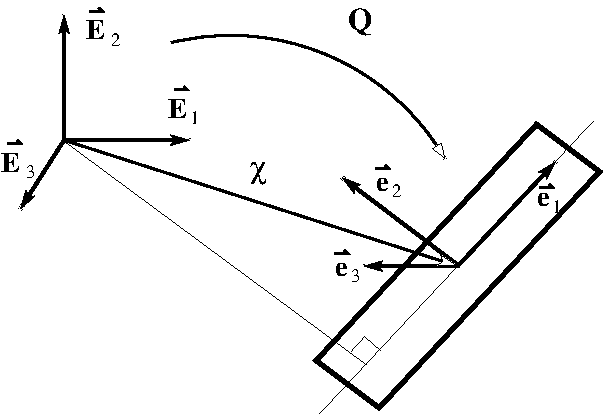
\includegraphics[width=8cm]{figures/chord.png}
    \caption{The co-ordinate system of a chord $( \vec{\mathbf{e}}_1 , \vec{\mathbf{e}}_2 , \vec{\mathbf{e}}_3 )$ relative to the co-ordinate system of its dodecahedron $( \vec{\mathbfsf{E}}_1 , \vec{\mathbfsf{E}}_2 , \vec{\mathbfsf{E}}_3 )$ with origins located at their respective centroids that are offset by a translation $\boldsymbol{\chi}$.  These describe a mapping $[ \{ \vec{\mathbf{e}}_1 \} \{ \vec{\mathbf{e}}_2 \} \{ \vec{\mathbf{e}}_3 \} ] = [ \{ \vec{\mathbf{E}}_1 \} \{ \vec{\mathbf{E}}_2 \} \{ \vec{\mathbf{E}}_3 \} ] [ \mathbfsf{Q} ]$ where $\mathbfsf{Q}$ is an orthogonal rotation.  The tangent base vector $\vec{\mathbf{e}}_1$ aligns with the axis of this chord. The normal base vector $\vec{\mathbf{e}}_2$ is coaxial with a line segment drawn from the origin out to the chordal axis such that $\vec{\mathbf{e}}_1 \cdot \vec{\mathbf{e}}_2 = 0$, while the binormal base vector is given by the cross product $\vec{\mathbf{e}}_3 = \vec{\mathbf{e}}_1 \times \vec{\mathbf{e}}_2$.}
    \label{figchord}
\end{figure}

\begin{figure}
    \centering
    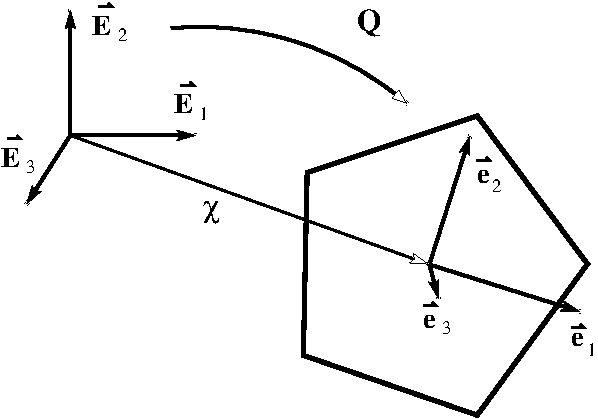
\includegraphics[width=8cm]{figures/pentagonCoord.png}
    \caption{The co-ordinate system of a pentagon $( \vec{\mathbf{e}}_1 , \vec{\mathbf{e}}_2 , \vec{\mathbf{e}}_3 )$ relative to the co-ordinate system of its dodecahedron $( \vec{\mathbfsf{E}}_1 , \vec{\mathbfsf{E}}_2 , \vec{\mathbfsf{E}}_3 )$ with origins located at their respective centroids that are offset by a translation $\boldsymbol{\chi}$.  These describe a mapping $[ \{ \vec{\mathbf{e}}_1 \} \{ \vec{\mathbf{e}}_2 \} \{ \vec{\mathbf{e}}_3 \} ] = [ \{ \vec{\mathbf{E}}_1 \} \{ \vec{\mathbf{E}}_2 \} \{ \vec{\mathbf{E}}_3 \} ] [ \mathbfsf{Q} ]$ where $\mathbfsf{Q}$ is an orthogonal rotation.  Base vector $\vec{\mathbf{e}}_1$ is coaxial to a line segment that connects two vertices which locate a pair of shoulders in a pentagon, viz., vertices 2 and 5 in Fig.~\ref{figRegPentagon}.  Base vector $\vec{\mathbf{e}}_2$ is coaxial with a line segment drawn from the head of this pentagon, i.e., vertex 1 in Fig.~\ref{figRegPentagon}, down to its base such that $\vec{\mathbf{e}}_1 \cdot \vec{\mathbf{e}}_2 = 0$.  Base vector $\vec{\mathbf{e}}_3 = \vec{\mathbf{e}}_1 \times \vec{\mathbf{e}}_2$ is the outward normal to this surface.}
    \label{figPentagonCoord}
\end{figure}

\begin{figure}
    \centering
    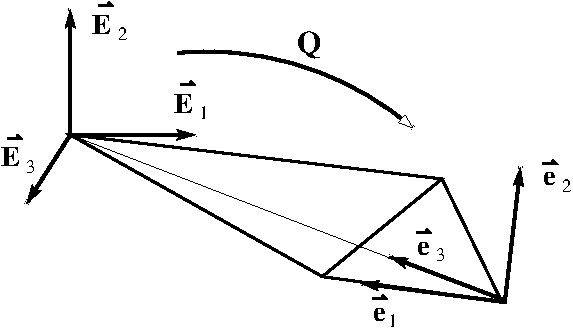
\includegraphics[width=8cm]{figures/tetrahedronCoord.png}
    \caption{The co-ordinate system of a tetrahedron $( \vec{\mathbf{e}}_1 , \vec{\mathbf{e}}_2 , \vec{\mathbf{e}}_3 )$ relative to the co-ordinate system of its dodecahedron $( \vec{\mathbfsf{E}}_1 , \vec{\mathbfsf{E}}_2 , \vec{\mathbfsf{E}}_3 )$ with origins located at their respective centroids.  These describe a mapping $[ \{ \vec{\mathbf{e}}_1 \} \{ \vec{\mathbf{e}}_2 \} \{ \vec{\mathbf{e}}_3 \} ] = [ \{ \vec{\mathbf{E}}_1 \} \{ \vec{\mathbf{E}}_2 \} \{ \vec{\mathbf{E}}_3 \} ] [ \mathbfsf{Q} ]$ where $\mathbfsf{Q}$ is an orthogonal rotation.  Base vector $\vec{\mathbf{e}}_1$ is coaxial to a line segment that connects the centroid of a pentagon with one of the pentagon's vertices.  Base vector  $\vec{\mathbf{e}}_2$ is normal to  $\vec{\mathbf{e}}_1$ and lies in the plane of the pentagon such that $\vec{\mathbf{e}}_1 \cdot \vec{\mathbf{e}}_2 = 0$.  Base vector $\vec{\mathbf{e}}_3 = \vec{\mathbf{e}}_1 \times \vec{\mathbf{e}}_2$ points toward the origin of the dodecahedron along the spine that connects the centroid of the dodecahedron with the centroid of a pentagon.  Vertex~1 is at the origin of $( \vec{\mathbf{e}}_1 , \vec{\mathbf{e}}_2 , \vec{\mathbf{e}}_3 )$.  Vertex~2 is along $\vec{\mathbf{e}}_1$.  Vertex~3 lies in the plane of the pentagon.  And vertex~4 is at the centroid of the dodecahedron $( \vec{\mathbfsf{E}}_1 , \vec{\mathbfsf{E}}_2 , \vec{\mathbfsf{E}}_3 )$.}
    \label{figTetrahedronCoord}
\end{figure}



%\setcounter{equation}{0}
%\setcounter{figure}{0}
%\setcounter{section}{0}
%\setcounter{table}{0}
\section{Kinematics}
\label{partKinematics}

The irregular dodecahedron used here as a model for alveoli describes a 3D structure comprising 30 1D rods (the septal chords) joined at 20 nodes (the vertices) that collectively circumscribe 12 2D pentagonal membranes (the alveolar septa) that in turn envelop an alveolar sac whose volume is represented using 60 tetrahedra.  To be able to describe the overall mechanical response of this 3D dodecahedral structure, it is conjectured to be sufficient to know the individual mechanical responses of its 1D septal chords, its 2D septal membranes, and the 3D void within.  Their relevant kinematics are presented here, along with the shape functions used for interpolation and their descriptions of deformation via stretch, using a Lagrangian measure for Laplace stretch \cite{Freedetal20} as our chosen kinematic field.

\subsection{$\,$1D Chords}

The stretch of a rod under extension is a ratio of its lengths.  Specifically, $\lambda \defeq L / L_0$ where $L$ and $L_0$ are its current and reference lengths, respectively, whose strain and strain rate are taken to be $e = \ln \lambda$ and $\mathrm{d} e = \lambda^{-1} \mathrm{d} \lambda$.  This is often referred to as a logarithmic, natural, or true strain.  Consequently, the kinematic analysis of a chord is trivial.

\subsubsection{Shape Functions for Interpolating a Rod}

A two-noded alveolar chord has shape functions $N_i$, $i=1,2$, that, when evaluated in its natural co-ordinate system where $-1 \leq \xi \leq 1$, describe a matrix with elements
\begin{subequations}
    \label{shapeFnsChord}
    \begin{align}
\mathbf{N} & = \begin{bmatrix} N_1 & N_2 \end{bmatrix} =
\begin{bmatrix}
\frac{1}{2} \, (1 - \xi) &  \frac{1}{2} \, (1 + \xi)
\end{bmatrix} \\
\intertext{that interpolate vector fields according to}
\mathbfit{x} ( \xi ) & = \sum_{i=1}^2 N_i ( \xi ) \, x_i , \quad
\mathbfit{u} ( \xi ) = \sum_{i=1}^2 N_i ( \xi ) \, u_i ,  \\
\intertext{etc., and whose spatial gradients are} 
N_{1,\xi} & = -\tfrac{1}{2} 
\quad \text{and} \quad
N_{2,\xi} = \tfrac{1}{2},
\end{align}
\end{subequations}
wherein $\xi$ is the natural co-ordinate.  Components $x_i$ and $u_i \defeq x_i - x_{0i}$, $i=1,2$, are their global co-ordinates and displacements, respectively, located at the two nodes of a chord evaluated in the co-ordinate frame $( \vec{\mathbfsf{e}}_1 , \vec{\mathbfsf{e}}_2 , \vec{\mathbfsf{e}}_3 )$ of Fig.~\ref{figchord} with the chordal axis lying in the $\vec{\mathbfsf{e}}_1$ direction.

\subsubsection{Deformation Gradient for a Rod}

The deformation gradient in this case is simply
\begin{multline}
    \mathbfsf{F} ( \xi ) = \mathbfsf{I} + \frac{\partial \mathbfit{u}}{\partial \xi} 
    \left( \frac{\partial \mathbfit{x}_0 }{\partial \xi} \right)^{-1} = 
  \mathbfsf{I} + \sum_{i=1}^2 N_{i,\xi} u_i \left( \sum_{i=1}^2 N_{i,\xi} x_{0i} \right)^{-1} \, \vec{\mathbfsf{e}}_1 \otimes \vec{\mathbfsf{e}}_1 \\
    = \mathbfsf{I} + \frac{u_2 - u_1}{x_{02} - x_{01}} \, \vec{\mathbfsf{e}}_1 \otimes \vec{\mathbfsf{e}}_1 = \frac{x_2 - x_1}{x_{02} - x_{01}} \, \vec{\mathbfsf{e}}_1 \otimes \vec{\mathbfsf{e}}_1,
\end{multline}
which is uniform over the length of a chord, i.e., it is independent of $\xi$.

\subsection{$\,$2D Triangles}

Triangular elements are needed in a support capacity in order to construct our alveolar model; specifically, the four surfaces of a tetrahedron are triangles.  What is required of them is a capability to compute the traction acting across such a surface through integration.  This requires knowledge of their shape functions and quadrature rules, the latter topic being discussed in Section~\ref{partNumericalMethods}. 

\subsubsection{Shape Functions for Interpolating a Triangle}

The shape functions for a triangle expressed in terms of its natural co-ordinates $( \xi , \eta )$, where $0 \leq \xi \leq 1$ and $0 \leq \eta \leq 1-\xi$, are given by
\begin{subequations}
    \label{triangleShapeFns}
    \begin{align}
    N_1 & = 1 - \xi - \eta &
    N_2 & = \xi &
    N_3 & = \eta 
    \intertext{with gradients of}
    N_{1,\xi} & = -1 & N_{2,\xi} & = 1 & N_{3,\xi} & = 0 \\
    N_{2,\eta} & = -1 & N_{2,\eta} & = 0 & N_{3,\eta} & = 1
    \end{align}
\end{subequations}
so that the area of a triangle in its natural co-ordinates is \textfrac{1}{2}.  

No further kinematics are required from triangular elements in our analysis.



\subsection{$\,$2D Irregular Pentagons}

The kinematics of an irregular pentagon, on the other hand, are not trivial.  Shape functions are required from which deformation gradients can then be constructed.  Once a deformation gradient is in hand, the state of stretch occurring within a pentagon at its Gauss points can finally be derived.  Several possible decompositions of the deformation gradient are possible, i.e., the notion of stretch is not unique in 2D (nor in 3D).  Here we employ the Lagrangian version of Laplace stretch \cite{Freedetal19}.

\subsubsection{Wachspress' Shape Functions for Interpolating an Irregular Pentagon}
\label{secShapeFns}

The idea here is to model each pentagonal face of a dodecahedron with one, pentagonal, finite element.  Five constant-strain triangles were originally considered, but their accuracy was found to be wanting when compared with that of a single pentagonal element whenever the deformation becomes non-uniform.  There was no difference between them whenever the deformation was just a uniform dilation.

In 1975, Wachspress \cite{Wachspress75,Wachspress16} derived a set of shape functions $N_i$ that are capable of interpolating convex polyhedra.  His shape functions take on the form of rational polynomials, viz., $N_i = A_i / B$ where $A_i$ and $B$ are polynomials.  In contrast, classic isoparametric elements are constructed from polynomial shape functions \cite{Hughes87}.  For the Wachspress shape functions of a pentagon, the $A_i$ are cubic polynomials, while $B$ is a quadratic polynomial.

Let us consider a convex pentagonal domain $\Omega$ defined over $\mathbb{R}^2$ whose vertices have global co-ordinates of
\begin{displaymath}
(x_1, y_1) , \; (x_2, y_2) , \; (x_3, y_3) , \; (x_4, y_4), \; (x_5, y_5)
\end{displaymath}
when evaluated in the pentagonal co-ordinate system $( \vec{\mathbfsf{e}}_1 , \vec{\mathbfsf{e}}_2 )$ of Fig.~\ref{figPentagonCoord}, with $\vec{\mathbfsf{e}}_3$ being an outward normal to the pentagon.  Associated with this set of global co-ordinates is a set of local or natural co-ordinates
\begin{displaymath}
(\xi_1 , \eta_1) , \; (\xi_2 , \eta_2) , \; (\xi_3 , \eta_3) , \; (\xi_4 , \eta_4) , \; (\xi_5 , \eta_5)
\end{displaymath}
that describe a mapping of interpolation where
\begin{equation}
\begin{aligned}
x(\xi, \eta) & = \sum\nolimits_{i=1}^5 N_i (\xi, \eta) \, x_i \\
y(\xi, \eta) & = \sum\nolimits_{i=1}^5 N_i (\xi, \eta) \, y_i
\end{aligned} 
\qquad \text{or} \qquad
\mathbfit{x}(\boldsymbol{\xi}) = \sum_{i=1}^5 N_i (\boldsymbol{\xi}) \, 
\mathbfit{x}_{\,i}
\end{equation}
which relate natural co-ordinates $\boldsymbol{\xi} \equiv (\xi, \eta)$ to global co-ordinates $\mathbfit{x} \equiv (x, y)$, where $\mathbfit{x}_{\,i} \equiv (x_i, y_i)$ are nodal co-ordinates at the $i^{\mathrm{th}}$ vertex, with $i$ indexing counter\-clockwise around a pentagon according to Fig.~\ref{figRegPentagon}.  Displacement $\mathbfit{u} (\mathbfit{x}) \defeq \mathbfit{x} - \mathbfit{x}_0$, with reference co-ordinates $\mathbfit{x}_0 \equiv (x_0, y_0)$, also obeys this mapping
\begin{equation}
\begin{aligned}
u(\xi, \eta) & = \sum\nolimits_{i=1}^5 N_i (\xi, \eta) \, u_i \\
v(\xi, \eta) & = \sum\nolimits_{i=1}^5 N_i (\xi, \eta) \, v_i
\end{aligned} 
\qquad \text{or} \qquad
\mathbfit{u}(\boldsymbol{\xi}) = \sum_{i=1}^5 N_i (\boldsymbol{\xi}) \, 
\mathbfit{u}_{\,i}
\end{equation}
whose components $\mathbfit{u}_{\,i} \equiv (u_i , v_i)$ designate the nodal displacements.

Shape functions $N_i (\boldsymbol{\xi}) \equiv N_i (\xi, \eta)$ are interpolation functions that place any position $P$ with local co-ordinates $\boldsymbol{\xi} \equiv (\xi, \eta) \in \widebar{\Omega}$, where $\widebar{\Omega} \defeq \Omega \cup \partial\Omega$, into their global co-ordinates $\mathbfit{x} \equiv (x,y)$.  The shape functions of Wachspress \cite{Wachspress75,Wachspress16} possess the following properties \cite{SukumarMalsch06}:
\begin{enumerate}
	\item Partition of unity: $\sum\nolimits_{i=1}^5 N_i (\boldsymbol{\xi}) = 1$, \; $0 \leq N_i (\boldsymbol{\xi}) \leq 1$.
	\item Interpolate nodal data: $N_i (\boldsymbol{\xi}_{\,j}) = \Xi_{ij}$.
	\item Linear completeness: $\sum\nolimits_{i=1}^5 N_i (\boldsymbol{\xi}) \, \mathbfit{x}_{\,i} = \mathbfit{x}$.
	\item For $\boldsymbol{\xi} \in \Omega$, $N_i (\boldsymbol{\xi})$ is $C^{\infty}$, but for $\boldsymbol{\xi} \in \partial \Omega$, $N_i (\boldsymbol{\xi})$ is $C^0$, i.e., interpolation is linear along an edge (or alveolar chord) connecting two neighboring vertices.
\end{enumerate}
Item 4 is often considered a disadvantage of Wachspress shape functions, viz., the linear interpolation along their boundaries.  However, this is appropriate for our modeling of alveoli, because the septal boundaries are alveolar chords that are taken to interpolate linearly.

For interpolating a convex, planar, pentagonal shape, the shape functions of Wachspress have polynomials of order three in their numerators, and another polynomial of order two in their denominators; specifically, we write them here as
\begin{subequations}
	\label{shapeFunctions}
	\begin{align}
	N_{i+1} (\xi, \eta) & = \kappa_i \, A_i (\xi, \eta) / B(\xi, \eta) , 
	\qquad i = 1, 2 , \dots , 5 \\ 
	\intertext{using a scaling factor of $\kappa_i$, where $N_1 \Leftarrow N_6$.  The numerators and denominator for interpolating a pentagon take on the general form of}
	A_i (\xi, \eta) & = \alpha_{0i} + \alpha_{1i} \xi + \alpha_{2i} \eta + 
	\alpha_{3i} \xi^2 + \alpha_{4i} \xi\eta + \alpha_{5i} \eta^2 \notag \\ 
	\mbox{} & \phantom{\mbox{} = \alpha_{0i}} + \alpha_{6i} \xi^3 + 
	\alpha_{7i} \xi^2 \eta + \alpha_{8i} \xi \eta^2 + \alpha_{9i} \eta^3 ,
	\label{shapeFnNum} \\
	B (\xi, \eta) & = \beta_0 + \beta_1 \xi + \beta_2 \eta + \beta_3 \xi^2 + 
	\beta_4 \xi\eta + \beta_5 \eta^2 ,
	\label{shapeFnDenom}
	\end{align}
\end{subequations}
where coefficients in the numerator, i.e., the $A_i$, differ with index $i$, while those in the denominator, viz., the $B \defeq \sum_{i=1}^5 A_i$, are the same for all five shape functions.  

We apply the construction technique of Dasgupta \cite{Dasgupta03} to compute the shape functions of Wachspress for an irregular convex pentagon.  Consider a chord $c_i$ that connects vertex $\mathbfit{\xi}_{\,i-1} = (\xi_{i-1} , \eta_{i-1})$ with vertex $\mathbfit{\xi}_{\,i} = (\xi_i , \eta_i)$ via a straight line segment such that $\ell_i = 0$ with $\ell_i \defeq 1 - a_{i} \xi - b_i \eta$ wherein
\begin{subequations}
	\begin{align}
	a_i & = \frac{\eta_i - \eta_{i-1}}{\xi_{i-1} \eta_i - \xi_i \eta_{i-1}}, \\
	b_i & = \frac{\xi_{i-1} - \xi_i}{\xi_{i-1} \eta_i - \xi_i \eta_{i-1}}, \\
	\intertext{for which Dasgupta derived the following set of constraints}
	\kappa_i & = \kappa_{i-1} \left( 
	\frac{a_{i+1} (\xi_{i-1} - \xi_i) + b_{i+1} (\eta_{i-1} - \eta_i)}
	{a_{i-1} (\xi_i - \xi_{i-1}) + b_{i-1} (\eta_i - \eta_{i-1})} \right) 
	\end{align}
\end{subequations}
with recursion starting at $\kappa_1 \defeq 1$.  Coefficients $\kappa_i$ enforce property 4 listed above.

With this information in hand, we then derived rational polynomials describing Wachspress' shape functions for a pentagon specified in Eq.~\ref{shapeFunctions} in terms of the parameters $a_i$, $b_i$, and $\kappa_i$.  The polynomial coefficients for the $A_i$ in Eq.~\ref{shapeFnNum} have values of
\begin{subequations}
	\label{shapeFnCoefs}
	\begin{align}
	\alpha_{0i} & = 1 \\
	\alpha_{1i} & = -( a_{i+1} + a_{i+2} + a_{i+3} ) \\
	\alpha_{2i} & = -( b_{i+1} + b_{i+2} + b_{i+3} ) \\
	\alpha_{3i} & = a_{i+1} a_{i+2} + a_{i+2} a_{i+3} + a_{i+3} a_{i+1} \\
	\alpha_{4i} & = a_{i+1} ( b_{i+2} + b_{i+3} ) + a_{i+2} ( b_{i+1} + 
	b_{i+3} ) + a_{i+3} ( b_{i+1} + b_{i+2} ) \\
	\alpha_{5i} & = b_{i+1} b_{i+2} + b_{i+2} b_{i+3} + b_{i+3} b_{i+1} \\
	\alpha_{6i} & = -a_{i+1} a_{i+2} a_{i+3} \\
	\alpha_{7i} & = -( a_{i+1} a_{i+2} b_{i+3} + a_{i+1} b_{i+2} a_{i+3} + 
	b_{i+1} a_{i+2} a_{i+3} ) \\
	\alpha_{8i} & = -( a_{i+1} b_{i+2} b_{i+3} + b_{i+1} a_{i+2} b_{i+3} + 
	b_{i+1} b_{i+2} a_{i+3} ) \\
	\alpha_{9i} & = -b_{i+1} b_{i+2} b_{i+3}
	\end{align}
\end{subequations}
which differ for each shape function via index $i = 1,2,\dots,5$, while the polynomial coefficients for $B$ in Eq.~\ref{shapeFnDenom} have values of
\begin{equation}
\beta_i = \sum_{j=1}^5 \alpha_{ij} \kappa_j, \qquad i = 0, 1, \dots, 5
\end{equation}
which are the same for all five shape functions.  Sums over the four cubic terms in Eq.~\ref{shapeFnCoefs} all vanish---a byproduct of Wachspress' formulation.  In the above formul\ae, an index count of $i \equiv 0 \implies i = 5$, while index counts of $i \equiv 6 \implies i = 1$, $i \equiv 7 \implies i = 2$, and $i \equiv 8 \implies i = 3$.  Shape function $N_1$ is illustrated in Fig.~\ref{figShapeFuntion}, with like images applying for the other four shape functions.

\begin{figure}
	\centering
	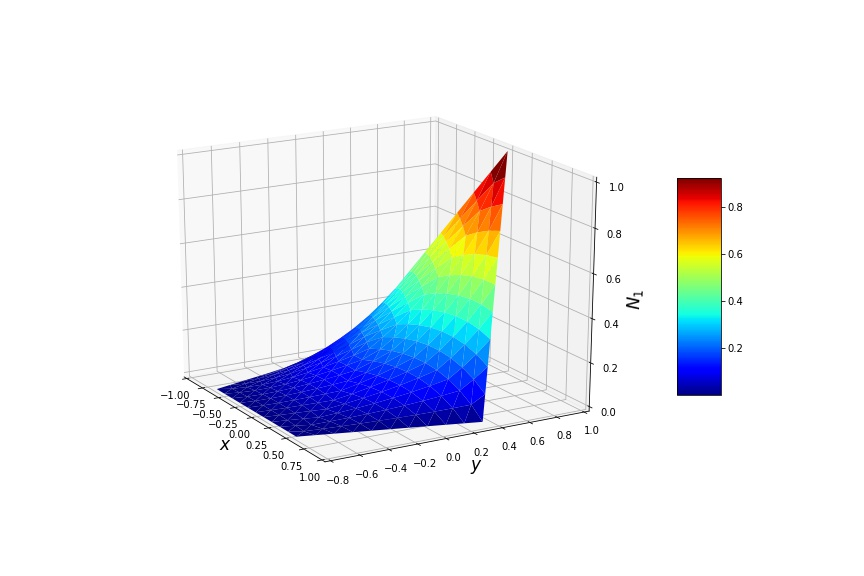
\includegraphics[width=0.9\textwidth]{figures/shapeFunction.jpg}
	\caption{Wachspress shape functions for a pentagon, in this case, shape function $N_1$}
	\label{figShapeFuntion}
\end{figure}

\subsubsection{First Derivatives of the Shape Functions}

The first derivatives of Wachspress' shape functions for a pentagon are
\begin{subequations}
    \label{shapeFunctionGradients}
	\begin{align}
	N_{i+1,\xi} (\xi, \eta) & = \kappa_i \, \mathcal{N}_{i,\xi}(\xi, \eta) /
	B^2(\xi, \eta), \\
	N_{i+1,\eta} (\xi, \eta) & = \kappa_i \, \mathcal{N}_{i,\eta}(\xi, \eta) /
	B^2(\xi, \eta), \\
	\intertext{where $N_{i+1,\xi}  (\xi, \eta) = \partial N_{i+1} (\xi, \eta) / \partial \xi$ and $N_{i+1,\eta} (\xi, \eta) = \partial N_{i+1} (\xi, \eta) / \partial \eta$ with}
	\mathcal{N}_{i,\xi} (\xi,\eta) & = B(\xi, \eta) A_{i,\xi} (\xi, \eta) -
	B_{,\xi} (\xi, \eta) A_i (\xi, \eta), \\
	\mathcal{N}_{i,\eta} (\xi,\eta) & = B(\xi, \eta) A_{i,\eta} (\xi, \eta) - 
	B_{,\eta} (\xi, \eta) A_i (\xi, \eta), \\
	\intertext{which contain the polynomials}
	A_{i,\xi} (\xi, \eta) & = \alpha_{1i} + 2 \alpha_{3i} \xi + \alpha_{4i} \eta +
	3 \alpha_{6i} \xi^2 + 2 \alpha_{7i} \xi \eta + \alpha_{8i} \eta^2,
	\label{shapeFnGradXiNum} \\
	A_{i,\eta} (\xi, \eta) & = \alpha_{2i} + \alpha_{4i} \xi + 2 \alpha_{5i} \eta + 
	\alpha_{7i} \xi^2 + 2 \alpha_{8i} \xi\eta + 3 \alpha_{9i} \eta^2 ,
	\label{shapeFnGradEtaNum} \\
	B_{,\xi} (\xi, \eta) & = \beta_1 + 2 \beta_3 \xi + \beta_4 \eta,
	\label{shapeFnGradXiDenom} \\
	B_{,\eta} (\xi, \eta) & = \beta_2 + \beta_4 \xi + 2 \beta_5 \eta ,
	\label{shapeFnGradEtaDenom}
	\end{align}
\end{subequations}
from which the deformation and displacement gradients are constructed.

\subsubsection{Second Derivatives of the Shape Functions}

The second derivatives of these shape functions, which we used to test the compatibility conditions of this element, are described by
\begin{subequations}
	\begin{align}
	N_{i+1,\xi\xi} & = \kappa_i \, \mathfrak{N}_{i,\xi\xi}(\xi,\eta) /
	B^3 (\xi,\eta), \\
	N_{i+1,\xi\eta} & = \kappa_i \, \mathfrak{N}_{i,\xi\eta}(\xi,\eta) /
	B^3(\xi,\eta), \\
	N_{i+1,\eta\xi} & = \kappa_i \, \mathfrak{N}_{i,\eta\xi}(\xi,\eta) /
	B^3(\xi,\eta), \\
	N_{i+1,\eta\eta} & = \kappa_i \, \mathfrak{N}_{i,\eta\eta}(\xi,\eta) /
	B^3(\xi,\eta), \\
	\intertext{where $N_{i+1,\xi\eta}  (\xi, \eta) = \partial^2 N_{i+1} (\xi, \eta) / \partial \xi \partial \eta$, etc., and  where}
	\mathfrak{N}_{i,\xi\xi} (\xi,\eta) & = B(\xi,\eta)
	\mathcal{N}_{i,\xi\xi} (\xi,\eta) - 2 B_{,\xi} (\xi,\eta) 
	\mathcal{N}_{i,\xi} (\xi,\eta), \\
	\mathfrak{N}_{i,\xi\eta}  (\xi,\eta)& = B(\xi,\eta) 
	\mathcal{N}_{i,\xi\eta} (\xi,\eta) - 2 B_{,\xi} (\xi,\eta) 
	\mathcal{N}_{i,\eta} (\xi,\eta), \\
	\mathfrak{N}_{i,\eta\xi}  (\xi,\eta)& = B(\xi,\eta)
	\mathcal{N}_{i,\eta\xi} (\xi,\eta) - 2 B_{,\eta} (\xi,\eta) 
	\mathcal{N}_{i,\xi} (\xi,\eta), \\
	\mathfrak{N}_{i,\eta\eta} (\xi,\eta) & = B(\xi,\eta) 
	\mathcal{N}_{i,\eta\eta} (\xi,\eta) - 2 B_{,\eta} (\xi,\eta) 
	\mathcal{N}_{i,\eta} (\xi,\eta), \\
	\intertext{wherein}
	\mathcal{N}_{i,\xi\xi} (\xi,\eta) & = B(\xi,\eta) A_{i,\xi\xi} (\xi,\eta) -
	B_{,\xi\xi} (\xi\eta) A_{i} (\xi\eta), \\
	\mathcal{N}_{i,\xi\eta} (\xi,\eta) & = B (\xi,\eta) A_{i,\xi\eta} (\xi,\eta) +
	B_{,\xi} (\xi,\eta) A_{i,\eta} (\xi,\eta) \notag \\
	\mbox{} & - B_{,\eta} (\xi,\eta) A_{i,\xi} (\xi,\eta) - 
	B_{,\xi\eta} (\xi,\eta) A_i (\xi,\eta), \\
	\mathcal{N}_{i,\eta\xi} (\xi,\eta) & = B (\xi,\eta) A_{i,\eta\xi} (\xi,\eta) +
	B_{,\eta} (\xi,\eta) A_{i,\xi} (\xi,\eta) \notag \\
	\mbox{} & - B_{,\xi} (\xi,\eta) A_{i,\eta} (\xi,\eta) - 
	B_{,\eta\xi} (\xi,\eta) A_i (\xi,\eta),  \\
	\mathcal{N}_{i,\eta\eta} (\xi,\eta) & = B(\xi,\eta) A_{i,\eta\eta} (\xi,\eta) -
	B_{,\eta\eta} (\xi,\eta) A_{i} (\xi,\eta), \\
	\intertext{which contain polynomials}
	A_{i,\xi\xi} (\xi,\eta) & = 2 \alpha_{3i} + 6 \alpha_{6i} \xi + 2 \alpha_{7i} \eta, \\
	A_{i,\xi\eta} (\xi,\eta) & = \alpha_{4i} + 2 \alpha_{7i} \xi + 2 \alpha_{8i} \eta, \\
	A_{i,\eta\eta} (\xi,\eta) & = 2 \alpha_{5i} + 2 \alpha_{8i} \xi + 6 \alpha_{9i} \eta, \\
	B_{,\xi\xi} (\xi,\eta) & = 2 \beta_3, \\
	B_{,\xi\eta} (\xi,\eta) & = \beta_4, \\
	B_{,\eta\eta} (\xi,\eta) & = 2 \beta_5,
	\end{align}
\end{subequations}
with $A_{i,\xi\eta} (\xi,\eta) = A_{i,\eta\xi} (\xi,\eta)$ and $B_{,\xi\eta} (\xi,\eta) = B_{,\eta\xi} (\xi,\eta)$. 

\subsubsection{Deformation Gradient for an Irregular Pentagon}

Derivatives of displacement $(u, v)$ taken with respect to the local co-ordinates $(\xi, \eta)$ described in terms of gradients of the shape functions $N_{i,\xi} (\xi, \eta)$ and $N_{i,\eta}(\xi, \eta)$ of a pentagon have components
\begin{subequations}
	\label{gradient}
	\begin{align}
	\begin{bmatrix}
	\partial u / \partial\xi & \partial u / \partial\eta \\
	\partial v / \partial\xi & \partial v / \partial\eta
	\end{bmatrix} & = 
	\begin{bmatrix}
	\sum\nolimits_{i=1}^5 N_{i,\xi} (\xi,\eta) \, u_i & \sum\nolimits_{i=1}^5 N_{i,\eta} (\xi,\eta) \, u_i \\
	\sum\nolimits_{i=1}^5 N_{i,\xi} (\xi,\eta) \, v_i & \sum\nolimits_{i=1}^5 N_{i,\eta} (\xi,\eta) \, v_i
	\end{bmatrix} ,
	\label{displacementGradients} \\
	\intertext{where $u \defeq x - x_0$ and $v \defeq y - y_0$.  Gradients of the global co-ordinates $(x_0,y_0)$ evaluated in a reference state taken with respect to the local co-ordinates $(\xi, \eta)$ have components} 
	\begin{bmatrix}
	\partial x_0 / \partial\xi & \partial x_0 / \partial\eta \\
	\partial y_0 / \partial\xi & \partial y_0 / \partial\eta
	\end{bmatrix} & = 
	\begin{bmatrix}
	\sum\nolimits_{i=1}^5 N_{i,\xi} (\xi,\eta) \, x_{0i} & \sum\nolimits_{i=1}^5 N_{i,\eta} (\xi,\eta) \, x_{0i} \\
	\sum\nolimits_{i=1}^5 N_{i,\xi} (\xi,\eta) \, y_{0i} & \sum\nolimits_{i=1}^5 N_{i,\eta} (\xi,\eta) \, y_{0i}
	\end{bmatrix},
	\label{co-ordinateGradients} \\
	\intertext{wherein $(x_{0i}, y_{0i})$ are the reference global co-ordinates at the $i^{\mathrm{th}}$ vertex, while gradients of the global co-ordinates $(x,y)$ evaluated in the current state taken with respect to the local co-ordinates $(\xi, \eta)$ have components}
	\begin{bmatrix}
	\partial x / \partial\xi & \partial x / \partial\eta \\
	\partial y / \partial\xi & \partial y / \partial\eta
	\end{bmatrix} & = 
	\begin{bmatrix}
	\sum\nolimits_{i=1}^5 N_{i,\xi} (\xi,\eta) \, x_i & \sum\nolimits_{i=1}^5 N_{i,\eta} (\xi,\eta) \, x_i \\
	\sum\nolimits_{i=1}^5 N_{i,\xi} (\xi,\eta) \, y_i & \sum\nolimits_{i=1}^5 N_{i,\eta} (\xi,\eta) \, y_i
	\end{bmatrix},
	\label{currentGradients} \\
    \intertext{whose transpose establishes the Jacobian matrix}
    \mathbf{J} \defeq \begin{bmatrix}
    \partial x / \partial\xi & \partial y / \partial\xi \\
    \partial x / \partial\eta & \partial y / \partial\eta
    \end{bmatrix} & = 
    \begin{bmatrix}
    \sum\nolimits_{i=1}^5 N_{i,\xi} (\xi,\eta) \, x_i & \sum\nolimits_{i=1}^5 N_{i,\xi} (\xi,\eta) \, y_i \\
    \sum\nolimits_{i=1}^5 N_{i,\eta} (\xi,\eta) \, x_i & \sum\nolimits_{i=1}^5 N_{i,\eta} (\xi,\eta) \, y_i
    \end{bmatrix},
    \label{JacobianMtx2D}
	\end{align}
\end{subequations}
wherein $(x_i, y_i)$ denote the current global co-ordinates at the $i^{\mathrm{th}}$ vertex.

From the above matrices, one can construct the deformation gradient $\mathbfsf{F} = \partial \mathbfit{x} / \partial \mathbf{x}_0 = \mathbfsf{I} + \partial \mathbfit{u} / \partial \mathbfit{x}_0$ for an irregular pentagon via
\begin{subequations}
    \label{deformationGradient}
    \begin{align}
\mathbfsf{F} (\xi, \eta) & = 
\begin{bmatrix}
F_{11}(\xi, \eta) & F_{12}(\xi, \eta) \\
F_{21}(\xi, \eta) & F_{22}(\xi, \eta)
\end{bmatrix} \notag \\ & = 
\begin{bmatrix}
1 & 0 \\
0 & 1
\end{bmatrix} + 
\begin{bmatrix}
\partial u / \partial \xi & \partial u / \partial \eta \\
\partial v / \partial \xi & \partial v / \partial \eta
\end{bmatrix}
\begin{bmatrix}
\partial x_0 / \partial \xi & \partial x_0 / \partial \eta \\
\partial y_0 / \partial \xi & \partial y_0 / \partial \eta
\end{bmatrix}^{-1} ,\\
\intertext{whose inverse is}
\mathbfsf{F}^{-1} (\xi, \eta) & =
\frac{1}{F_{11} (\xi, \eta) F_{22} (\xi, \eta) - 
    F_{21} (\xi, \eta) F_{12} (\xi, \eta)}
\begin{bmatrix}
F_{22} (\xi, \eta) & -F_{12} (\xi, \eta) \\
-F_{21} (\xi, \eta) & F_{11} (\xi, \eta)
\end{bmatrix},
\end{align}
\end{subequations}
while its associated displacement gradient $\mathbfsf{G} = \partial \mathbfit{u} / \partial \mathbfit{x}$ is given by
\begin{equation}
\mathbfsf{G} (\xi, \eta) = 
\begin{bmatrix}
G_{11}(\xi, \eta) & G_{12}(\xi, \eta) \\
G_{21}(\xi, \eta) & G_{22}(\xi, \eta)
\end{bmatrix} 
\mbox{} = 
\begin{bmatrix}
\partial u / \partial \xi & \partial u / \partial \eta \\
\partial v / \partial \xi & \partial v / \partial \eta
\end{bmatrix}
\begin{bmatrix}
\partial x / \partial \xi & \partial x / \partial \eta \\
\partial y / \partial \xi & \partial y / \partial \eta
\end{bmatrix}^{-1} ,
\label{displacementGradient}
\end{equation}
which is not invertible, in general.  All are evaluated in the 12 plane belonging to a co-ordinate system $( \vec{\mathbfsf{e}}_2 , \vec{\mathbfsf{e}}_2 , \vec{\mathbfsf{e}}_3 )$ that orients this pentagon, with $\vec{\mathbfsf{e}}_3$ being normal to its surface, as illustrated in Fig.~\ref{figPentagonCoord}.  The deformation and displacement gradients are two, fundamental, kinematic fields commonly used in the construction of constitutive equations.

\subsubsection{Compatibility Conditions}

To ensure that a deformation is compatible, and therefore integrable, it follows that the curl of its deformation gradient must be zero \cite{Clayton15}.  This condition is trivially satisfied for the shape functions that we use for 1D chords, 2D triangles, and 3D tetrahedra.  However, for the Wachspress shape function used to interpolate pentagons, this needs to be verified.  Vanishing of the curl of $\mathbfsf{F}$ results in two constraint equations for the planar case, they being
\begin{equation}
\label{compatibility}
F_{11,2} = F_{12,1} 
\qquad \text{and} \qquad
F_{22,1} = F_{21,2}
\end{equation}
whose spatial derivatives associate with the $( \vec{\mathbfsf{e}}_1 , \vec{\mathbfsf{e}}_2 )$ co-ordinate frame.

From Eq.~\ref{deformationGradient}, it follows that the spatial derivatives of the deformation gradient are
\begin{multline}
\mathbfsf{F}_{,1} (\xi, \eta) = \frac{\partial}{\partial x_0}
\begin{bmatrix}
F_{11}(\xi, \eta) & F_{12}(\xi, \eta) \\
F_{21}(\xi, \eta) & F_{22}(\xi, \eta)
\end{bmatrix} \\ 
\mbox{} = \frac{\partial \xi}{\partial x_0} \left( \frac{\partial}{\partial \xi} \left(
\begin{bmatrix}
\partial u / \partial \xi & \partial u / \partial \eta \\
\partial v / \partial \xi & \partial v / \partial \eta
\end{bmatrix} \right)
\begin{bmatrix}
\partial x_0 / \partial \xi & \partial x_0 / \partial \eta \\
\partial y_0 / \partial \xi & \partial y_0 / \partial \eta
\end{bmatrix}^{-1} -
\begin{bmatrix}
\partial u / \partial \xi & \partial u / \partial \eta \\
\partial v / \partial \xi & \partial v / \partial \eta
\end{bmatrix} \right. \\ \times \left.
\begin{bmatrix}
\partial x_0 / \partial \xi & \partial x_0 / \partial \eta \\
\partial y_0 / \partial \xi & \partial y_0 / \partial \eta
\end{bmatrix}^{-1}
\frac{\partial}{\partial \xi} \left(
\begin{bmatrix}
\partial x_0 / \partial \xi & \partial x_0 / \partial \eta \\
\partial y_0 / \partial \xi & \partial y_0 / \partial \eta
\end{bmatrix} \right)
\begin{bmatrix}
\partial x_0 / \partial \xi & \partial x_0 / \partial \eta \\
\partial y_0 / \partial \xi & \partial y_0 / \partial \eta
\end{bmatrix}^{-1} \right)
\addtocounter{equation}{1}
\tag{\theequation a}
\end{multline}
and
\begin{multline}
\mathbfsf{F}_{,2} (\xi, \eta) = \frac{\partial}{\partial y_0}
\begin{bmatrix}
F_{11}(\xi, \eta) & F_{12}(\xi, \eta) \\
F_{21}(\xi, \eta) & F_{22}(\xi, \eta)
\end{bmatrix} \\ 
\mbox{} = \frac{\partial \eta}{\partial y_0} \left(
\frac{\partial}{\partial \eta} \left(
\begin{bmatrix}
\partial u / \partial \xi & \partial u / \partial \eta \\
\partial v / \partial \xi & \partial v / \partial \eta
\end{bmatrix} \right)
\begin{bmatrix}
\partial x_0 / \partial \xi & \partial x_0 / \partial \eta \\
\partial y_0 / \partial \xi & \partial y_0 / \partial \eta
\end{bmatrix}^{-1} -
\begin{bmatrix}
\partial u / \partial \xi & \partial u / \partial \eta \\
\partial v / \partial \xi & \partial v / \partial \eta
\end{bmatrix} \right. \\ \times \left.
\begin{bmatrix}
\partial x_0 / \partial \xi & \partial x_0 / \partial \eta \\
\partial y_0 / \partial \xi & \partial y_0 / \partial \eta
\end{bmatrix}^{-1}
\frac{\partial}{\partial \eta} \left(
\begin{bmatrix}
\partial x_0 / \partial \xi & \partial x_0 / \partial \eta \\
\partial y_0 / \partial \xi & \partial y_0 / \partial \eta
\end{bmatrix} \right)
\begin{bmatrix}
\partial x_0 / \partial \xi & \partial x_0 / \partial \eta \\
\partial y_0 / \partial \xi & \partial y_0 / \partial \eta
\end{bmatrix}^{-1} \right)
\tag{\theequation b}
\end{multline}
wherein
\begin{subequations}
	\begin{align}
	\frac{\partial}{\partial \xi}
	\begin{bmatrix}
	\partial u / \partial\xi & \partial u / \partial\eta \\
	\partial v / \partial\xi & \partial v / \partial\eta
	\end{bmatrix} & = 
	\begin{bmatrix}
	\sum\nolimits_{i=1}^5 N_{i,\xi\xi} (\xi,\eta) \, u_i & \sum\nolimits_{i=1}^5 N_{i,\xi\eta} (\xi,\eta) \, u_i \\
	\sum\nolimits_{i=1}^5 N_{i,\xi\xi} (\xi,\eta) \, v_i & \sum\nolimits_{i=1}^5 N_{i,\xi\eta} (\xi,\eta) \, v_i
	\end{bmatrix} \\
	\frac{\partial}{\partial \eta}
	\begin{bmatrix}
	\partial u / \partial\xi & \partial u / \partial\eta \\
	\partial v / \partial\xi & \partial v / \partial\eta
	\end{bmatrix} & = 
	\begin{bmatrix}
	\sum\nolimits_{i=1}^5 N_{i,\eta\xi} (\xi,\eta) \, u_i & \sum\nolimits_{i=1}^5 N_{i,\eta\eta} (\xi,\eta) \, u_i \\
	\sum\nolimits_{i=1}^5 N_{i,\eta\xi} (\xi,\eta) \, v_i & \sum\nolimits_{i=1}^5 N_{i,\eta\eta} (\xi,\eta) \, v_i 
	\end{bmatrix} \\
	\intertext{and}
	\frac{\partial}{\partial \xi}
	\begin{bmatrix}
	\partial x_0 / \partial\xi & \partial x_0 / \partial\eta \\
	\partial y_0 / \partial\xi & \partial y_0 / \partial\eta
	\end{bmatrix} & = 
	\begin{bmatrix}
	\sum\nolimits_{i=1}^5 N_{i,\xi\xi} (\xi,\eta) \, x_{0i} & \sum\nolimits_{i=1}^5 N_{i,\xi\eta} (\xi,\eta) \, x_{0i} \\
	\sum\nolimits_{i=1}^5 N_{i,\xi\xi} (\xi,\eta) \, y_{0i} & \sum\nolimits_{i=1}^5 N_{i,\xi\eta} (\xi,\eta) \, y_{0i}
	\end{bmatrix} \\
	\frac{\partial}{\partial \eta}
	\begin{bmatrix}
	\partial x_0 / \partial\xi & \partial x_0 / \partial\eta \\
	\partial y_0 / \partial\xi & \partial y_0 / \partial\eta
	\end{bmatrix} & = 
	\begin{bmatrix}
	\sum\nolimits_{i=1}^5 N_{i,\eta\xi} (\xi,\eta) \, x_{0i} & \sum\nolimits_{i=1}^5 N_{i,\eta\eta} (\xi,\eta) \, x_{0i} \\
	\sum\nolimits_{i=1}^5 N_{i,\eta\xi} (\xi,\eta) \, y_{0i} & \sum\nolimits_{i=1}^5 N_{i,\eta\eta} (\xi,\eta) \, y_{0i}
	\end{bmatrix}
	\end{align}
\end{subequations}
with $\partial \xi / \partial x_0$ and $\partial \eta / \partial y_0$ effectively being scaling factors that we take to be described as a ratio of septal chord lengths; specifically, let
\begin{equation}
\frac{\partial \xi}{\partial x_0} \simeq
\frac{\partial \eta}{\partial y_0} \approx 
\frac{L(\xi, \eta)}{L_0 (x, y)} = 
\frac{\cos (\omega)}{\sqrt{A_0 / 5 \tan (\omega)}},
\end{equation}
where $L(\xi,\eta)$ is the septal length of a pentagonal edge in its natural configuration, as drawn in Fig.~\ref{figRegPentagon}, while $L_0(x,y)$ is the actual, alveolar, septal length with $A_0(x,y)$ being the area of an alveolar septum in its reference state.  This formula follows from Eqs.~\ref{regPentagonLength} and \ref{regPentagonArea}.

\textbf{Note}: We study compatibility only for the purpose of assessing applicability in our choice of selecting Wachspress shape functions.  Otherwise, it is not required in our modeling of an alveolus via a dodecahedron. 

\subsubsection{Gram--Schmidt Decomposition of the Deformation Gradient}
\label{secQR}

To describe kinematics of a planar membrane, an upper-triangular Gram--Schmidt decomposition of the deformation gradient $\mathbfsf{F}$ is used in lieu of the symmetric polar decomposition that is commonly adopted \cite{Srinivasa12,FreedSrinivasa15,Freedetal17,FreedZamani19,Freedetal19}.  McLellan \cite{McLellan76,McLellan80} was the first to propose a triangular decomposition of $\mathbfsf{F}$, to prove its uniqueness and existence, and to establish many of its physical properties.  This idea has been rediscovered several times since then. \cite{Rosakis90,Souchet93,Srinivasa12}  A thorough history of the \textbf{QR} (Gram--Schmidt) decomposition has been written by Leon \textit{et~al}.\ \cite{Leonetal13}, with a brief history regarding its application to kinematics being given in Freed \textit{et~al}. \cite{Freedetal19}  Compatibility conditions have been analyzed in the context of \textbf{QR} kinematics for mechanics problems in two \cite{claytonMRC20} and three \cite{PaulFreed20} spatial dimensions.

A Lagrangian Gram--Schmidt factorization of the deformation gradient $\mathbfsf{F}$ is written here as $\mathbfsf{F} = \boldsymbol{\mathcal{RU}}$, where the rotation $\boldsymbol{\mathcal{R}}$ is orthogonal and the Laplace stretch $\boldsymbol{\mathcal{U}}$ is upper-triangular \cite{Freedetal19}.\footnote{
	The \textbf{QR} rotation $\boldsymbol{\mathcal{R}}$ and stretch $\boldsymbol{\mathcal{U}}$ tensors are distinct from those that arise from a polar decomposition of a deformation gradient, typically denoted as $\mathbfsf{R}$ and $\mathbfsf{U}$, as found in any, modern, continuum mechanics text.  McLellan \cite{McLellan76,McLellan80} introduced the Laplace stretch in 1976, which he denoted as $\mathbfsf{H}$, while Srinivasa \cite{Srinivasa12} denoted it as $\tilde{\mathbfsf{F}}$ in his 2012 paper.
} 
(An Eulerian Gram--Schmidt factorization has just been derived, \cite{Freedetal20} but it came along too late to adopt in this study.  Its application is a topic for future study.)  This triangular measure of stretch possesses an inherent property in two space: the direction aligned with the rotated 1-axis, denoted as $\vec{\mathbfit{g}}_{\hspace{0.5pt}1}$, remains invariant under transformation $\boldsymbol{\mathcal{U}}$ \cite{McLellan80}, i.e., it is a material vector in a neighborhood surrounding that particle whereat $\mathbfsf{F}$ is evaluated \cite{FreedZamani18}.  This property has some interesting ramifications addressed in \S\ref{secDilemma}.

\paragraph{\textbf{QR} Factorization of\/ $\mathbfsf{F}$}
\label{secQR2D}

The $2 \times 2$ deformation gradient associated with a planar membrane has a Gram--Schmidt decomposition expressed in terms of four physical attributes.  Three of these attributes describe deformation.  They are defined as \cite{Freedetal17}
\begin{equation}
a = \sqrt{F_{11}^{\,2} + F_{21}^{\,2}} , \quad
b = \frac{F_{11} F_{22} - F_{12} F_{21}}
{\sqrt{F_{11}^{\,2} + F_{21}^{\,2}}} , \quad
g = \frac{F_{11} F_{12} +  F_{22} F_{21}}
{F_{11}^{\,2} + F_{21}^{\,2}} ,
\label{physicalVariables}
\end{equation}
thereby populating Laplace stretch $\boldsymbol{\mathcal{U}}$ and its inverse $\boldsymbol{\mathcal{U}}^{-1}$ with components
\begin{equation}
\boldsymbol{\mathcal{U}} = \begin{bmatrix}
a & a g \\ 0 & b
\end{bmatrix} \qquad \text{and} \qquad
\boldsymbol{\mathcal{U}}^{-1} = \begin{bmatrix} 
1 / a & -g / b \\ 0 & 1 / b
\end{bmatrix},
\label{LaplaceStretch2D}
\end{equation}
where $a$ and $b$ are the principal elongations (ratios of current lengths to reference lengths) and $g$ is the extent of in-plane shear, as measured in a co-ordinate frame $(  \vec{\mathbfsf{g}}_1 , \vec{\mathbfsf{g}}_2 )$ illustrated in Fig.~\ref{figKinematics}.  It is worth pointing out that the components of Laplace stretch, viz., $\mathcal{U}_{ij}$, are evaluated in the reference co-ordinate system $( \vec{\mathbfsf{e}}_1 , \vec{\mathbfsf{e}}_2 )$ of the pentagon, as $\mathbfsf{F} = F_{ij} \, \vec{\mathbfsf{e}}_i \otimes \vec{\mathbfsf{e}}_j$, but their physical interpretations arise in the Gram rotated co-ordinate system $( \vec{\mathbfsf{g}}_1 , \vec{\mathbfsf{g}}_2 )$.

\begin{figure}
	\centering
	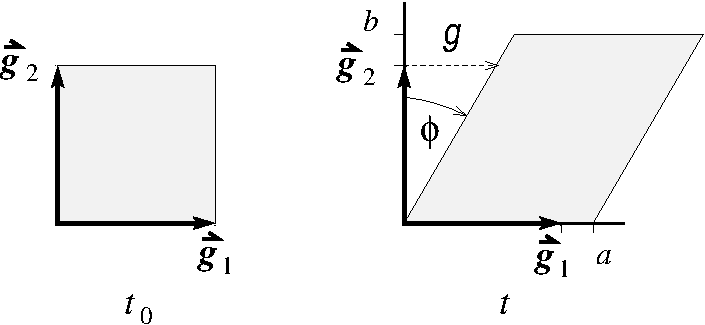
\includegraphics[width=8cm]{figures/deformation.png}
	\caption{Physical attributes of a planar deformation: $a$ and $b$ represent elongations, while $g = \tan \phi$ denotes the magnitude of shear.  They are measured in a physical frame of reference with unit base vectors $( \vec{\mathbfsf{g}}_1 , \vec{\mathbfsf{g}}_2 )$ where $\vec{\mathbfsf{g}}_1$ embeds in the material.}
	\label{figKinematics}
\end{figure}

Orthogonal tensor $\boldsymbol{\mathcal{R}} = \bigl[ \vec{\mathbfsf{g}}_1 \bigm| \vec{\mathbfsf{g}}_2 \bigr] = \delta_{ij} \, \vec{\mathbfsf{g}}_i \otimes \vec{\mathbfsf{e}}_j = \mathcal{R}_{ij} \, \vec{\mathbfsf{e}}_i \otimes \vec{\mathbfsf{e}}_j$ rotates the reference co-ordinate axes $( \vec{\mathbfsf{e}}_1 , \vec{\mathbfsf{e}}_2 )$ into a physical co-ordinate system $( \vec{\mathbfsf{g}}_1 , \vec{\mathbfsf{g}}_2 )$ through an angle $\theta$, which is the fourth physical attribute arising from a \textbf{QR} factorization of $\mathbfsf{F}$.  This angle of rotation describes a proper orthogonal matrix, specifically
\begin{equation}
\boldsymbol{\mathcal{R}} = \begin{bmatrix}
\cos \theta & -\sin \theta \\
\sin \theta & \cos \theta
\end{bmatrix} ,
\label{rotation}
\end{equation}  
with
\begin{equation}
\sin \theta = \frac{F_{21}}
{\sqrt{F_{11}^{\,2} + F_{21}^{\,2}}} , \quad
\cos \theta = \frac{F_{11}}
{\sqrt{F_{11}^{\,2} + F_{21}^{\,2}}} 
\quad \therefore \quad
\theta = \tan^{-1} \left( \frac{F_{21}}{F_{11}} \right)
\label{trigFns}
\end{equation}  
where a positive angle $\theta$ corresponds with a counter\-clockwise rotation of physical axes $( \vec{\mathbfsf{g}}_1 , \vec{\mathbfsf{g}}_2 )$ about reference axes $( \vec{\mathbfsf{e}}_1 , \vec{\mathbfsf{e}}_2 )$.  

From the four independent components of a planar deformation gradient $F_{ij}$ come three deformation attributes, i.e., $a$, $b$, and $g$, and one rotational attribute, i.e., $\theta$.


\paragraph{Dilemma}
\label{secDilemma} 

Until recently, \cite{Pauletal20} there has been a tacit assumption in prior applications of Gram--Schmidt factorizations of $\mathbfsf{F}$. Specifically, the physical base vectors $( \vec{\mathbfsf{g}}_1 , \vec{\mathbfsf{g}}_2 )$ satisfy a geometric condition whereby the physical 1-direction $\vec{\mathbfsf{g}}_1$ rotates out of the reference 1-direction $\vec{\mathbfsf{e}}_1$, but this need not always be the case.  Physical vector $\vec{\mathbfsf{g}}_1$ could equally likely rotate out of the 2-direction $\vec{\mathbfsf{e}}_2$ of the reference frame.  At issue is not: How the physical base vectors orient in space?  That is managed by Gram's procedure.  Rather, at issue is: How do the physical base vectors index with respect to the reference base vectors?  This topic is addressed in \S\ref{reindexing3D} for the 3D case; below, we address this topic for the 2D case.

To illustrate the concern, consider two deformation histories, as drawn in Fig.~\ref{figDilemma}, each of which describes a simple shear taking place in the plane of a membrane.  In one case shear occurs in the 1-direction, while in the other case shear occurs in the 2-direction.  There are no elongations in either deformation considered.  These motions lead to different Gram--Schmidt factorizations of the deformation gradient.  When following the protocol of Eqs.~\ref{physicalVariables}--\ref{trigFns}, these factorizations are found to be
\begin{subequations}
	\label{shears}
	\begin{align}
	\mathbfsf{F} = 
	\begin{bmatrix} 1 & \gamma \\ 0 & 1 \end{bmatrix} & \implies 
	\boldsymbol{\mathcal{R}} = 
	\begin{bmatrix} 1 & 0 \\ 0 & 1 \end{bmatrix} , \quad
	\boldsymbol{\mathcal{U}} = 
	\begin{bmatrix} 1 & \gamma \\ 0 & 1  \end{bmatrix} 
	\label{shear1} \\
	\intertext{and}
	\mathbfsf{F} = 
	\begin{bmatrix} 1 & 0 \\ \gamma & 1 \end{bmatrix} & \implies \left\{
	\begin{aligned} \mbox{}
	\boldsymbol{\mathcal{R}} & = \frac{1}{\sqrt{1 + \gamma^2}}
	\begin{bmatrix} 1 & -\gamma \\ \gamma & 1 \end{bmatrix} \\
	\boldsymbol{\mathcal{U}} & = 
	\begin{bmatrix} \sqrt{1 + \gamma^2} & \gamma \\ 
	0 & 1 \bigm/ \sqrt{1 + \gamma^2} \end{bmatrix}
	\end{aligned} \right.
	\label{shear2}
	\end{align}
\end{subequations}
respectively, where we see that shear $\mathcal{U}_{12}$ has the same physical interpretation in both cases, viz., $\gamma$, but elongations $\mathcal{U}_{11}$ and $\mathcal{U}_{22}$ do not, viz., $\mathcal{U}_{11}=1$ and $\mathcal{U}_{22}=1$ in Eq.~\ref{shear1}, whereas $\mathcal{U}_{11} = \sqrt{1 + \gamma^2}$ and $\mathcal{U}_{22} = 1 / \sqrt{1 + \gamma^2}$ for the motion described in Eq.~\ref{shear2}.  Consequently, two geometric interpretations are produced for just one physical mode of deformation.  This cannot be!

\begin{figure}
	\centering
	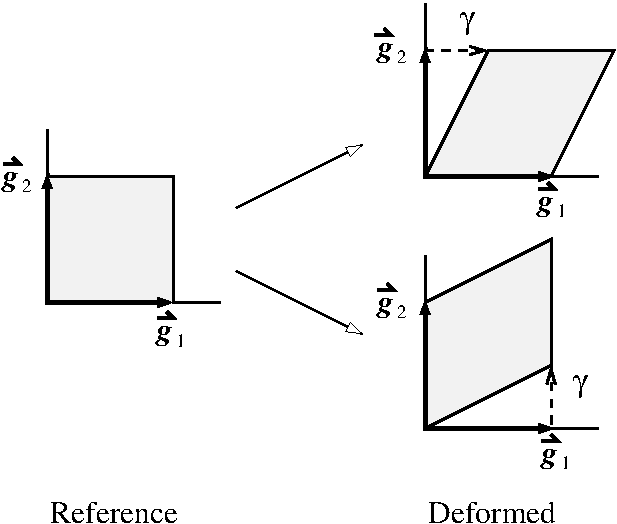
\includegraphics[width=0.5\textwidth]{figures/figDilemma.png}
	\caption{The left graphic designates a reference configuration while the right two graphics designate deformed configurations, both in basis $( \vec{\mathbfsf{g}}_1 , \vec{\mathbfsf{g}}_2 )$.  The top graphic associates with the motion of Eq.~\ref{shear1}, while the bottom graphic associates with the motion of Eq.~\ref{shear2}.}
	\label{figDilemma}
\end{figure}

The only difference between the motions that lead to the two deformation gradients presented in Eq.~\ref{shears} is one's choice for labeling the co-ordinate directions.  Matrix operations of row and column pivoting, taken from linear algebra, allow one to transform the lower-triangular form of Eq.~\ref{shear2} into an upper-triangular form like Eq.~\ref{shear1}; hence, producing an unified physical interpretation for both shearing motions, and thereby providing a means for establishing a remedy to this dilemma. 


\paragraph{Remedy}
\label{secRemedy}

For 2D membranes, there are only two co-ordinate re-indexings that are possible (for 3D solids there are six, cf.\ \S\ref{reindexing3D}).  The default is no re-indexing at all, in which case 
\begin{subequations}
	\label{membraneRelabling}
	\begin{align}
	[ \mathbfsf{P} ] = [ \mathbfsf{P}_0 ] & \defeq 
	\begin{bmatrix} 1 & 0 \\ 0 & 1 \end{bmatrix} & 
	\implies & & \begin{bmatrix}
	\mathcal{F}_{11} & \mathcal{F}_{12} \\
	\mathcal{F}_{21} & \mathcal{F}_{22}
	\end{bmatrix} & \defeq \begin{bmatrix}
	F_{11} & F_{12} \\
	F_{21} & F_{22}
	\end{bmatrix} \label{Q0} \\
	\intertext{while in the second case there is a re-indexing specified by}
	[ \mathbfsf{P} ] = [ \mathbfsf{P}_1 ] & \defeq 
	\begin{bmatrix} 0 & 1 \\ 1 & 0 \end{bmatrix} & 
	\implies & & \begin{bmatrix}
	\mathcal{F}_{11} & \mathcal{F}_{12} \\
	\mathcal{F}_{21} & \mathcal{F}_{22}
	\end{bmatrix} & \defeq \begin{bmatrix}
	F_{22} & F_{21} \\
	F_{12} & F_{11}
	\end{bmatrix}
	\label{Q1}
	\end{align}
\end{subequations}
where components $\mathcal{F}_{ij} = P_{ki} F_{k\ell} P_{\ell j}$ are the components to be used in the Gram--Schmidt factorization presented in \S\ref{secQR2D}, see also \S\ref{reindexing3D}, and where $\mathbfsf{P} \in \{ \mathbfsf{P}_0 , \mathbfsf{P}_1 \}$ is orthogonal, i.e., $\mathbfsf{P} \mathbfsf{P}^{\mathsf{T}} = \mathbfsf{P}^{\hspace{-1pt}\mathsf{T}} \mathbfsf{P} = \mathbfsf{I}$ with $\det \mathbfsf{P} = \pm 1$; specifically, $\det \mathbfsf{P}_0 = +1$ while $\det \mathbfsf{P}_1 = -1$.

The challenge in implementing such a strategy is to determine when to switch from $\mathbfsf{P}_0$ (case 1) to $\mathbfsf{P}_1$ (case 2), or back again, viz., from $\mathbfsf{P}_1$ to $\mathbfsf{P}_0$.  Continuity in the physical fields of deformation $(a , b , g )$ must be satisfied in order for such a change in co-ordinate frame to be physically meaningful.  To this end, it is useful to represent the components of a planar deformation gradient as
\begin{equation}
\begin{bmatrix}
\mathcal{F}_{11} & \mathcal{F}_{12} \\
\mathcal{F}_{21} & \mathcal{F}_{22}
\end{bmatrix} =
\begin{cases}
\mathrm{case} \; 1: & \begin{bmatrix}
F_{11} & F_{12} \\
F_{21} & F_{22}
\end{bmatrix}_{\vphantom{|}} = \begin{bmatrix}
x & \beta y \\ \alpha x & y
\end{bmatrix} \\
\mathrm{case} \; 2: & \begin{bmatrix}
F_{22} & F_{21} \\
F_{12} & F_{11}
\end{bmatrix} = \begin{bmatrix}
y & \alpha x \\ \beta y & x
\end{bmatrix}
\end{cases}
\label{deformationGradientRelabelling}
\end{equation}
where $x = F_{11}$ and $y = F_{22}$ are elongations, while ratios $\alpha = F_{21} / F_{11}$ and $\beta = F_{12} / F_{22}$ are magnitudes of shear, as illustrated in Fig.~\ref{figF}.  

\begin{figure}
	\centering
	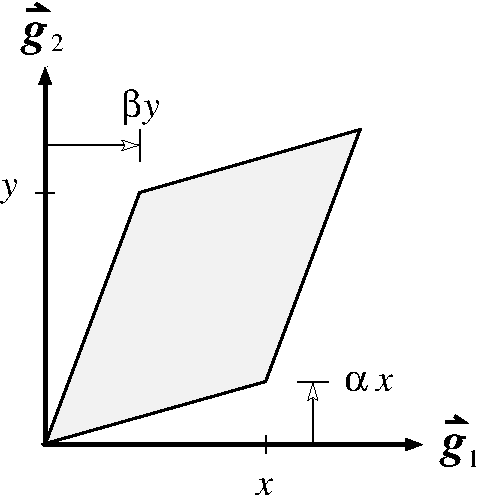
\includegraphics[width=0.3\textwidth]{figures/figF.png}
	\caption{A general description for homogeneous planar deformation, where $x , y \in \mathbb{R}_+$ and $\alpha , \beta \in \mathbb{R}$.  Shears $\alpha$ and $\beta$ are drawn in their positive sense.}
	\label{figF}
\end{figure}

The physical attributes for Laplace stretch, as they pertain to the two cases in Eq.~\ref{membraneRelabling}, written in terms of components $F_{ij}$ from $\mathbfsf{F} = F_{ij} \, \vec{\mathbfsf{e}}_i \otimes \vec{\mathbfsf{e}}_j$ as defined in Eq.~\ref{deformationGradientRelabelling}, are respectively given by
\begin{subequations}
	\label{physicalAttributes}
	\begin{align}
	\tilde{a} & = x \sqrt{1 + \alpha^2} & 
	\hat{a} & = y \sqrt{1 + \beta^2} 
	\label{aAttribute} \\
	\tilde{b} & = y ( 1 - \alpha \beta ) \bigm/ \sqrt{1 + \alpha^2} &
	\hat{b} & = x ( 1 - \alpha \beta ) \bigm/ \sqrt{1 + \beta^2} 
	\label{bAttribute} \\ 
	\tilde{g} & = y ( \alpha + \beta ) \bigm/ x (1 + \alpha^2) &
	\hat{g} & = x ( \alpha + \beta ) \bigm/ y (1 + \beta^2)
	\label{gAttribute} \\
	\tilde{\theta} & = \tan^{-1} ( -\alpha ) & 
	\hat{\theta} & = \tan^{-1} ( -\beta )
	\label{thetaAttribute}
	\end{align}
\end{subequations}
where attributes in the left column apply to case~1 (i.e., Eq.~\ref{Q0}) while those in the right column apply to case~2 (viz., Eq.~\ref{Q1}).  The actual set of physical attributes $\{ a, b, g, \theta \}$ that are to be used when quantifying Laplace stretch and its inverse, according to Eq.~\ref{LaplaceStretch2D}, are then selected via the strategy  
\begin{subequations}
	\label{attributeMaps}
	\begin{align}
	\mathrm{if} \; | \tilde{g} | \geq | \hat{g} | : & &
	\{ \tilde{a} , \tilde{b} , \tilde{g} , \tilde{\theta} \} &
	\mapsto \{ a , b , g , \theta \}  \\
	\mathrm{else} \; | \tilde{g} | \leq | \hat{g} | : & &
	\{ \hat{a} , \hat{b} , \hat{g} , \hat{\theta} \} & 
	\mapsto \{ a , b , g , \theta \},
	\end{align}
\end{subequations}
where it is easily verified that $\tilde{a} = \hat{a}$ and $\tilde{b} = \hat{b}$ whenever $\tilde{g} = \hat{g}$; consequently, the physical attributes of deformation $a , b , g$ remain continuous across a co-ordinate switch, however, the angle of co-ordinate rotation $\theta$ will not be continuous across such a switch between co-ordinate frames, as they represent rotations out of different co-ordinate directions.  A like statement applies in the 3D case whenever one uses the re-indexing scheme presented in \S\ref{reindexing3D}, i.e., the physical attributes of Laplace stretch remain continuous across a re-indexing of one's co-ordinate frame \cite{Pauletal20}.

The above strategy returns matrices for the rotation and Laplace stretch described in Eq.~\ref{shear1} for both deformation gradients presented in Eq.~\ref{shears}. The dilemma is remedied.  Laplace stretch, as remedied, therefore has an unique physical interpretation.    Co-ordinate re-indexing ensures that the invariant properties of Laplace stretch \cite{McLellan80} are adhered to.

The above protocol is the 2D version of the 3D version \cite{Pauletal20} presented in \S\ref{reindexing3D}.  It is easier to understand what is happening in the 2D case, which is why more detail is presented here.  It may certainly happen that even when the 3D co-ordinates for the dodecahedron are re-indexed, there may be one or more of the 12 pentagons whose 2D co-ordinates need to be re-indexed, too.

There are three kinematic variables that describe deformation in a planar membrane: elongation ratios $a$ and $b$ and simple shear $g$.  These variables will vary both temporally and spatially throughout a pentagon whenever Wachspress' shape functions are used.

\subsubsection{Thermodynamic Strains and Strain Rates}
\label{strainsAndStrainRates2D}

In terms of the above physical attributes for stretch, i.e., $a$, $b$, and $g$, and their reference values, viz., $a_0$, $b_0$, and $g_0$, one can define a set of strain attributes derived from thermo\-dynamics, specifically \cite{Freed17}
\begin{subequations}
    \label{thermodynamicStrains2D}
    \begin{align}
    \xi & \defeq \ln \left( \sqrt{\frac{a}{a_0} \frac{b}{b_0}} \right) & 
    \mathrm{d} \xi & = \frac{1}{2} \left( \frac{\mathrm{d}a}{a} + 
    \frac{\mathrm{d}b}{b} \right) \\
    \varepsilon & \defeq \ln \left( \sqrt{\frac{a}{a_0} \frac{b_0}{b}} \right) &
    \mathrm{d} \varepsilon & = \frac{1}{2} \left( \frac{\mathrm{d}a}{a} - 
    \frac{\mathrm{d}b}{b} \right) \\
    \gamma & \defeq g - g_0 & 
    \mathrm{d} \gamma & = \mathrm{d} g
    \end{align}
\end{subequations}
whose rates are exact differentials, i.e., they are independent of path---a tacit requirement from thermo\-dynamics \cite{Caratheodory09}.  Here $\xi$ denotes a dilation (uniform areal stretch), $\varepsilon$ denotes a squeeze (pure shear), and $\gamma$ denotes a (simple) shear. 

\paragraph{Stretch Rates}

The following approximations for stretch rates were derived by Freed and Zamani \cite{FreedZamani18}.  From these, the various strain rates listed in Eq.~\ref{thermodynamicStrains2D} can be established.  

A forward difference formula is used to approximate rates in the reference configuration for the various stretch attributes, as obtained from $\mathrm{d}\boldsymbol{\mathcal{U}}_0 = ( \boldsymbol{\mathcal{U}}_1 -  \boldsymbol{\mathcal{U}}_0 ) / \mathrm{d}t + \mathcal{O}(\mathrm{d}t)$ that, neglecting higher-order terms, produces
\begin{equation}
\mathrm{d} a_0 = \frac {a_1 - a_0}{\mathrm{d}t} , \quad 
\mathrm{d} b_0 = \frac {b_1 - b_0}{\mathrm{d}t} , \quad 
\mathrm{d} g_0 = \frac{a_1}{a_0} 
\left( \frac{g_1 - g_0}{\mathrm{d}t} \right) ,
\label{forwardDifference1stOrder2D}
\end{equation}
where $\mathrm{d} t = t_1 - t_0$ is the applied time step.  A backward difference formula $\mathrm{d} \boldsymbol{\mathcal{U}}_1 = ( \boldsymbol{\mathcal{U}}_1 - \boldsymbol{\mathcal{U}}_0 ) / \mathrm{d}t + \mathcal{O}(\mathrm{d}t)$ is used to estimate rates for the various stretch attributes at the end of its first integration step that, neglecting higher-order terms, give
\begin{equation}
\mathrm{d} a_1 = \frac {a_1 - a_0}{\mathrm{d}t} , \quad
\mathrm{d} b_1 = \frac {b_1 - b_0}{\mathrm{d}t} , \quad
\mathrm{d} g_1 = \frac{a_0}{a_1} 
\left(\frac{g_1 - g_0}{\mathrm{d}t} \right) .
\label{backwardDifference1stOrder2D}
\end{equation}
Curiously, there is a distinction in how the shear rates are approximated at the two nodes for this first interval of integration.

Equations \ref{forwardDifference1stOrder2D} and \ref{backwardDifference1stOrder2D} are first-order approximations for these derivatives.  Second-order approximations can be established whenever $i > 0$ provided the stepsize for step $[i, i+1]$ equals the stepsize for step $[i-1, i]$, where state $i=0$ associates with an initial condition.  The backward difference formula  $\mathrm{d} \boldsymbol{\mathcal{U}}_{i+1} = ( 3 \, \boldsymbol{\mathcal{U}}_{i+1} -  4 \, \boldsymbol{\mathcal{U}}_{i} + \boldsymbol{\mathcal{U}}_{i-1} ) / 2\mathrm{d}t + \mathcal{O} \bigl( (\mathrm{d}t)^2 \bigr)$ then produces rates for the stretch attributes of
\begin{equation}
\begin{aligned}
\mathrm{d} a_{i+1} & 
= \frac {3a_{i+1} - 4a_i +  a_{i-1}}{2\mathrm{d}t} \\ 
\mathrm{d} b_{i+1} & 
= \frac {3b_{i+1} - 4b_i +  b_{i-1}}{2\mathrm{d}t} \\
\mathrm{d} g_{i+1} & 
= \frac{2a_i} {a_{i+1}} \left(\frac{g_{i+1} - g_{i}}{\mathrm{d}t} \right) - \frac{a_{i-1}}{a_{i+1}} \left( \frac{g_{i+1} - g_{i-1}}{2\mathrm{d}t} \right) ,
\end{aligned}
\label{backwardDifference2ndOrder2D}
\end{equation}
which require stretch attributes $a_{i-1}$, $b_{i-1}$, and $g_{i-1}$ to be stored in a finite element setting.


\subsection{$\,$3D Irregular Dodecahedra}

The primary kinematic variables needed to describe the deformation of an irregular dodecahedron used as a model for an alveolar sac are its volume $V$ (see \S\ref{sec:geometries}) and the differential change in volume $\mathrm{d}V$, with the former following from Eq.~\ref{tetrahedralVolume} and the latter coming from a suitable finite difference formula.  Whenever the material filling an alveolar sac is air (its normal healthy condition), no further breakdown of these kinematics is required.  

However, whenever an alveolar sac is filled with fluid (blood, interstitial fluids, pflem, etc.), this fluid can be expected to behave solid-like in the face of a passing shock wave.  In this situation, the non-uniform measures for strain (i.e., shears) can be expected to produce non-uniform responses in stress.

\subsubsection{Shape Functions for Interpolating an Irregular Tetrahedron}

The shape functions associated with the four vertices of a tetrahedron $N_i$, $i = 1, 2, 3, 4,$ are defined as
\begin{subequations}
    \begin{align}
    N_1 & = 1 - \xi - \eta - \zeta , \quad
    N_2 = \xi , \quad
    N_3 = \eta , \quad
    N_4 = \zeta, \\
    \intertext{where $\xi$, $\eta$ and $\zeta$ represent natural co-ordinates with $0 \leq \xi \leq 1$, $0 \leq \eta \leq 1-\xi$ and $0 \leq \zeta \leq 1-\xi-\eta$.  Gradients of these shape functions are} 
    N_{1,\xi} & = -1 , \quad N_{1,\eta} = -1 , \quad N_{1,\zeta} = -1 \notag \\
    N_{2,\xi} & = 1 , \quad \phantom{-} N_{2,\eta} = 0 , \quad \phantom{-} N_{2,\zeta} = 0 \notag \\
    N_{3,\xi} & = 0 , \quad \phantom{-} N_{3,\eta} = 1 , \quad \phantom{-} N_{3,\zeta} = 0 \notag \\
    N_{4,\xi} & = 0 , \quad \phantom{-} N_{4,\eta} = 0 , \quad \phantom{-} N_{4,\zeta} = 1 
    \end{align}
\end{subequations}
and consequently the deformation gradient will be constant throughout its volume, like the deformation gradients used for chords and triangles.

\paragraph{Deformation Gradient for an Irregular Tetrahedron}

The deformation gradient for a volume element is constructed from
\small
\begin{equation}
\mathbfsf{F} ( \xi , \eta , \zeta ) = \begin{bmatrix} 1 & 0 & 0 \\
0 & 1 & 0 \\ 0 & 0 & 1 \end{bmatrix} + \begin{bmatrix}
\partial u / \partial \xi & \partial u / \partial \eta & \partial u / \partial \zeta \\
\partial v / \partial \xi & \partial v / \partial \eta & \partial v / \partial \zeta \\
\partial w / \partial \xi & \partial w / \partial \eta & \partial w / \partial \zeta
\end{bmatrix} \begin{bmatrix}
\partial x_0 / \partial \xi & \partial x_0 / \partial \eta & \partial x_0 / \partial \zeta \\
\partial y_0 / \partial \xi & \partial y_0 / \partial \eta & \partial y_0 / \partial \zeta \\
\partial z_0 / \partial \xi & \partial z_0 / \partial \eta & \partial z_0 / \partial \zeta
\end{bmatrix}^{-1}
\end{equation}
\normalsize
such that, for the four-node tetrahedron considered here, one has
\begin{subequations}
    \begin{align}
    \begin{bmatrix}
    \partial u / \partial \xi & \partial u / \partial \eta & \partial u / \partial \zeta \\
    \partial v / \partial \xi & \partial v / \partial \eta & \partial v / \partial \zeta \\
    \partial w / \partial \xi & \partial w / \partial \eta & \partial w / \partial \zeta
    \end{bmatrix} & = \begin{bmatrix}
    \sum_{i=1}^4 N_{i,\xi} u_i & \sum_{i=1}^4 N_{i,\eta} u_i & \sum_{i=1}^4 N_{i,\zeta} u_i \\
    \sum_{i=1}^4 N_{i,\xi} v_i & \sum_{i=1}^4 N_{i,\eta} v_i & \sum_{i=1}^4 N_{i,\zeta} v_i \\
    \sum_{i=1}^4 N_{i,\xi} w_i & \sum_{i=1}^4 N_{i,\eta} w_i & \sum_{i=1}^4 N_{i,\zeta} w_i 
    \end{bmatrix} \notag \\
    & = \begin{bmatrix}
    u_2 - u_1 & u_3 - u_1 & u_4 - u_1 \\
    v_2 - v_1 & v_3 - v_1 & v_4 - v_1 \\
    w_2 - w_1 & w_3 - w_1 & w_4 - w_1
    \end{bmatrix} \\
    \intertext{whose nodal displacements $\mathbfit{u}_i \defeq \mathbfit{x}_i - \mathbfit{x}_{0i}$, $i=1,2,3,4$, have components of $\mathbfit{u}_i = u_i \, \vec{\mathbfsf{E}}_1 + v_i \, \vec{\mathbfsf{E}}_2 + w_i \, \vec{\mathbfsf{E}}_3$  with $u_i \defeq x_i - x_{0i}$, $v_i \defeq y_i - y_{0i}$, and $w_i \defeq z_i - z_{0i}$, evaluated in the reference co-ordinate frame $( \vec{\mathbfsf{E}}_1 , \vec{\mathbfsf{E}}_2 , \vec{\mathbfsf{E}}_3 )$ of the dodecahedron, and}
    \begin{bmatrix}
    \partial x_0 / \partial \xi & \partial x_0 / \partial \eta & \partial x_0 / \partial \zeta \\
    \partial y_0 / \partial \xi & \partial y_0 / \partial \eta & \partial y_0 / \partial \zeta \\
    \partial z_0 / \partial \xi & \partial z_0 / \partial \eta & \partial z_0 / \partial \zeta
    \end{bmatrix} & = \begin{bmatrix}
    \sum_{i=1}^4 N_{i,\xi} x_{0i} & \sum_{i=1}^4 N_{i,\eta} x_{0i} & \sum_{i=1}^4 N_{i,\zeta} x_{0i} \\
    \sum_{i=1}^4 N_{i,\xi} y_{0i} & \sum_{i=1}^4 N_{i,\eta} y_{0i} & \sum_{i=1}^4 N_{i,\zeta} y_{0i} \\
    \sum_{i=1}^4 N_{i,\xi} z_{0i} & \sum_{i=1}^4 N_{i,\eta} z_{0i} & \sum_{i=1}^4 N_{i,\zeta} z_{0i}
    \end{bmatrix} \notag \\
    & = \begin{bmatrix}
    x_{02} - x_{01} & x_{03} - x_{01} & x_{04} - x_{01} \\
    y_{02} - y_{01} & y_{03} - y_{01} & y_{04} - y_{01} \\
    z_{02} - z_{01} & z_{03} - z_{01} & z_{04} - z_{01}
    \end{bmatrix} \\
    \intertext{whose initial nodal positions are $\mathbfit{x}_{0i} = x_{0i} \, \vec{\mathbfsf{E}}_1 + y_{0i} \, \vec{\mathbfsf{E}}_2 + z_{0i} \, \vec{\mathbfsf{E}}_3$ at vertex $i$.  This matrix is invertible, because the four vertices of a tetrahedron are distinct.  The Jacobian matrix is therefore given by}
    \mathbf{J} \defeq \begin{bmatrix}
    \partial x / \partial \xi & \partial y / \partial \xi & \partial z / \partial \xi \\
    \partial x / \partial \eta & \partial y / \partial \eta & \partial z / \partial \eta \\
    \partial x / \partial \zeta & \partial y / \partial \zeta & \partial z / \partial \zeta
    \end{bmatrix} & = \begin{bmatrix}
    \sum_{i=1}^4 N_{i,\xi} x_{i} & \sum_{i=1}^4 N_{i,\xi} y_{i} & \sum_{i=1}^4 N_{i,\xi} z_{i} \\
    \sum_{i=1}^4 N_{i,\eta} x_{i} & \sum_{i=1}^4 N_{i,\eta} y_{i} & \sum_{i=1}^4 N_{i,\eta} z_{i} \\
    \sum_{i=1}^4 N_{i,\zeta} x_{i} & \sum_{i=1}^4 N_{i,\zeta} y_{i} & \sum_{i=1}^4 N_{i,\zeta} z_{i}
    \end{bmatrix} \notag \\
    & = \begin{bmatrix}
    x_{2} - x_{1} & y_{2} - y_{1} & z_{2} - z_{1} \\
    x_{3} - x_{1} & y_{3} - y_{1} & z_{3} - z_{1} \\
    x_{4} - x_{1} & y_{4} - y_{1} & z_{4} - z_{1}
    \end{bmatrix}
    \label{tetJacobian}
    \end{align}
\end{subequations}
whose determinant is used in integrations.  The current nodal positions have components $\mathbfit{x}_{i} = x_i \, \vec{\mathbfsf{E}}_1 + y_i \, \vec{\mathbfsf{E}}_2 + z_i \, \vec{\mathbfsf{E}}_3$, $i=1,2,3,4$, in the dodecahedral frame $( \vec{\mathbfsf{E}}_1 , \vec{\mathbfsf{E}}_2 , \vec{\mathbfsf{E}}_3 )$.  The Jacobian matrix remains invertible provided that the four vertices of a tetrahedron remain distinct.

\subsubsection{\textbf{QR} Factorization of $\mathbfsf{F}$}
\label{secQR3D}

The re-indexed deformation gradient presented in \S\ref{reindexing3D} has a Gram--Schmidt decomposition that we denote as $\mathbfsf{F} = \boldsymbol{\mathcal{RU}}$ whose components are an orthogonal rotation matrix $\boldsymbol{\mathcal{R}} = \bigl[ \vec{\mathbfsf{g}}_1 \bigm| \vec{\mathbfsf{g}}_2 \bigm| \vec{\mathbfsf{g}}_3 \bigr] = \delta_{ij} \, \vec{\mathbfsf{g}}_i \otimes \vec{\mathbfsf{E}}_j = \mathcal{R}_{ij} \, \vec{\mathbfsf{E}}_i \otimes \vec{\mathbfsf{E}}_j$ and an upper-triangular matrix $\boldsymbol{\mathcal{U}} = \mathcal{U}_{ij} \, \vec{\mathbfsf{E}}_i \otimes \vec{\mathbfsf{E}}_j$ called Laplace stretch, \cite{Freedetal19} both evaluated in the reference co-ordinate frame $( \vec{\mathbfsf{E}}_1 , \vec{\mathbfsf{E}}_2 , \vec{\mathbfsf{E}}_3 )$, so that $\mathbfsf{F} = \mathcal{F}_{ij} \, \vec{\mathbfsf{E}}_i \otimes \vec{\mathbfsf{E}}_j = \mathcal{R}_{ik\,} \mathcal{U}_{kj} \, \vec{\mathbfsf{E}}_i \otimes \vec{\mathbfsf{E}}_j$, and therefore $\mathcal{F}_{ij} = \mathcal{R}_{ik\,} \mathcal{U}_{kj}$.

The components of Laplace stretch $\mathcal{U}_{ij}$ are readily gotten through a Cholesky factorization of the right Cauchy--Green deformation tensor $\mathbfsf{C} = \mathcal{C}_{ij} \, \vec{\mathbfsf{E}}_i \otimes \vec{\mathbfsf{E}}_j$ with tensor components $\mathcal{C}_{ij} = \mathcal{F}_{ki\,} \mathcal{F}_{kj}$ that relate to their physical attributes via \cite{Freed17}
\begin{equation} 
\boldsymbol{\mathcal{U}} = 
\begin{bmatrix}
a & a \gamma & a \beta \\ 0 & b & b \alpha \\ 0 & 0 & c
\end{bmatrix} 
\quad \text{with inverse} \quad
\boldsymbol{\mathcal{U}}^{-1} = \begin{bmatrix}
1/a & -\gamma / b & -( \beta - \alpha\gamma ) / c \\
0 & 1/b & -\alpha / c \\
0 & 0 & 1/c
\end{bmatrix}
\label{LaplaceStretch3D}
\end{equation}
with tensor components $\mathcal{U}_{ij}$ being evaluated according to formul\ae\ \cite{Srinivasa12}
\begin{equation}
\begin{aligned}
\mathcal{U}_{11} & = \sqrt{\mathcal{C}_{11}} & 
\mathcal{U}_{12} & = \mathcal{C}_{12} / \mathcal{U}_{11} &
\mathcal{U}_{13} & = \mathcal{C}_{13} / \mathcal{U}_{11} \\
\mathcal{U}_{21} & = 0 &
\mathcal{U}_{22} & = \sqrt{\mathcal{C}_{22} - \mathcal{U}_{12}^{\,2}} &
\mathcal{U}_{23} & = \bigl( \mathcal{C}_{23} - 
\mathcal{U}_{12\,} \mathcal{U}_{13} \bigr) / \mathcal{U}_{22} \\
\mathcal{U}_{31} & = 0 &
\mathcal{U}_{32} & = 0 & 
\mathcal{U}_{33} & = \sqrt{\mathcal{C}_{33} - \mathcal{U}_{13}^{\,2} - 
    \mathcal{U}_{23}^{\,2}}
\end{aligned}
\label{LagrangianLaplaceStretch3D}
\end{equation}
implying that the physical attributes for Laplace stretch can be evaluated via
\begin{equation}
a \defeq \mathcal{U}_{11} , \quad
b \defeq \mathcal{U}_{22} , \quad
c \defeq \mathcal{U}_{33} , \quad
\alpha \defeq \frac{\mathcal{U}_{23}}{\mathcal{U}_{22}} , \quad
\beta \defeq \frac{\mathcal{U}_{13}}{\mathcal{U}_{11}} , \quad
\gamma \defeq \frac{\mathcal{U}_{12}}{\mathcal{U}_{11}},
\label{LagrangianPhysicalAttributes3D}
\end{equation}
where $a$, $b$, and $c$ are three, orthogonal, elongation ratios, and where $\alpha$, $\beta$, and $\gamma$ are three, orthogonal, simple shears, with $a_0$, $b_0$, $c_0$, $\alpha_0$, $\beta_0$, and $\gamma_0$ denoting their values in some reference state. The elongations must be positive, whereas the shears may be of either sign. Collectively, they constitute a complete set of physical attributes for describing stretch from which constitutive equations can then be constructed. 

No eigen\-value\slash eigen\-vector analysis is required to acquire either the stretch components or their attributes when using this technique. \cite{Srinivasa12} The eigen\-values and eigen\-vectors of the triangular Laplace stretch equate with the eigen\-values and eigen\-vectors of the symmetric polar stretch \textit{only\/} in an absence of shear. \cite{Rosakis90}  Laplace stretch associates with the geometric description of a cube deforming into a parallelepiped; whereas, polar stretch associates with the geometric description of a sphere deforming into an ellipsoid.  They are distinct geometric measures for stretch.

\subsubsection{Thermodynamic Strains and Strain Rates}
\label{strainsAndStrainRates3D}

In terms of the above physical attributes for stretch, one can define an useful set of strain attributes derived from thermo\-dynamics, specifically \cite{Freed17}
\begin{subequations}
    \label{thermodynamicStrains3D}
    \begin{align}
    \Xi & \defeq \ln \left( \sqrt[3]{\frac{a}{a_0} \frac{b}{b_0} \frac{c}{c_0}} \right) & 
    \mathrm{d} \Xi & = \frac{1}{3} \left( \frac{\mathrm{d}a}{a} + 
    \frac{\mathrm{d}b}{b} + \frac{\mathrm{d}c}{c} \right) \\
    \varepsilon_1 & \defeq \ln \left( \sqrt[3]{\frac{a}{a_0} \frac{b_0}{b}} \right) &
    \mathrm{d} \varepsilon_1 & = \frac{1}{3} \left( \frac{\mathrm{d}a}{a} - 
    \frac{\mathrm{d}b}{b} \right) \\
    \varepsilon_2 & \defeq \ln \left( \sqrt[3]{\frac{b}{b_0} \frac{c_0}{c}} \right) &
    \mathrm{d} \varepsilon_2 & = \frac{1}{3} \left( \frac{\mathrm{d}b}{b} - 
    \frac{\mathrm{d}c}{c} \right) \\
    \gamma_1 & \defeq \alpha - \alpha_0 & 
    \mathrm{d} \gamma_1 & = \mathrm{d} \alpha \\
    \gamma_2 & \defeq \beta - \beta_0 & 
    \mathrm{d} \gamma_2 & = \mathrm{d} \beta \\
    \gamma_3 & \defeq \gamma - \gamma_0 & 
    \mathrm{d} \gamma_3 & = \mathrm{d} \gamma
    \end{align}
\end{subequations}
whose rates are exact differentials, i.e., they are independent of path---a tacit requirement from thermo\-dynamics \cite{Caratheodory09}.  Here $\Xi$ represents dilatation, $\varepsilon_1$ is a squeeze in the 12~plane, and $\varepsilon_2$ is a squeeze in the 23~plane, while $\gamma_1$ is a shear in the 23~plane, $\gamma_2$ is a shear in the 13~plane, and $\gamma_3$ is a shear in the 12~plane, which are three, orthogonal, simple shearing motions.  There is a third squeeze, too, viz., $\varepsilon_3 = -\varepsilon_1 - \varepsilon_2$, but it is not an independent descriptor of strain.

\paragraph{Stretch Rates}

The following approximations for stretch rates were derived by Freed and Zamani \cite{FreedZamani18}.  From these, the various strain rates listed in Eq.~\ref{thermodynamicStrains3D} can be established.  

A forward difference formula is used to approximate rates in the reference configuration for the various stretch attributes, as obtained from $\mathrm{d} \boldsymbol{\mathcal{U}}_0 = ( \boldsymbol{\mathcal{U}}_1 -  \boldsymbol{\mathcal{U}}_0 ) / \mathrm{d}t + \mathcal{O}(\mathrm{d}t)$.  Neglecting higher-order terms, this produces
\begin{equation}
\begin{aligned}
\mathrm{d} a_0 &
= \frac {a_1 - a_0}{\mathrm{d}t} \quad &
\mathrm{d} \alpha_0 & 
= \frac{b_1}{b_0} \left(\frac{\alpha_1 - \alpha_0}{\mathrm{d}t} \right) \\
\mathrm{d} b_0 & 
= \frac {b_1 - b_0}{\mathrm{d}t} \quad & 
\mathrm{d} \beta_0 & 
= \frac{a_1}{a_0} \left( \frac{\beta_1 - \beta_0}{\mathrm{d}t} \right) \\
\mathrm{d} c_0 & 
= \frac {c_1 - c_0}{\mathrm{d}t} \quad & 
\mathrm{d} \gamma_0 & = \frac{a_1}{a_0} \left( \frac{\gamma_1 - \gamma_0}{\mathrm{d}t}\right) .
\end{aligned}
\label{forwardDifference1stOrder3D}
\end{equation}
A backward difference formula $\mathrm{d} \boldsymbol{\mathcal{U}}_1 = ( \boldsymbol{\mathcal{U}}_1 -  \boldsymbol{\mathcal{U}}_0 ) / \mathrm{d}t + \mathcal{O}(\mathrm{d}t)$ is used to estimate rates for the various stretch attributes at the end of its first integration step, from which it follows that
\begin{equation}
\begin{aligned}
\mathrm{d} a_1 & 
= \frac {a_1 - a_0}{\mathrm{d}t} \;\; & 
\mathrm{d} \alpha_1 & 
= \frac {b_0}{b_1} \left( \frac{\alpha_1 - \alpha_0}{\mathrm{d}t} \right) \\
\mathrm{d} b_1 & 
= \frac {b_1 - b_0}{\mathrm{d}t} \;\; & 
\mathrm{d} \beta_1 & 
= \frac {a_0} {a_1} \left( \frac{\beta_1 - \beta_0}{\mathrm{d}t} \right) \\
\mathrm{d} c_1 & 
= \frac {c_1 - c_0}{\mathrm{d}t} \;\; & 
\mathrm{d} \gamma_1 & 
= \frac{a_0}{a_1} \left(\frac{\gamma_1 - \gamma_0}{\mathrm{d}t} \right) .
\end{aligned}
\label{backwardDifference1stOrder3D}
\end{equation}
Curiously, there is a distinction in how the shear rates are approximated at the two nodes belonging to this first interval of integration.

Equations \ref{forwardDifference1stOrder3D} and \ref{backwardDifference1stOrder3D} are first-order approximations for these derivatives.  Second-order approximations can be established whenever $i > 0$ provided the stepsize for step $[i, i+1]$ equals the stepsize for step $[i-1, i]$, where state $i=0$ associates with an initial condition.  The backward difference formula  $\mathrm{d} \boldsymbol{\mathcal{U}}_{i+1} = ( 3 \, \boldsymbol{\mathcal{U}}_{i+1} -  4 \, \boldsymbol{\mathcal{U}}_i + \boldsymbol{\mathcal{U}}_{i-1} ) / 2\mathrm{d}t + \mathcal{O} \bigl( ( \mathrm{d}t )^2 \bigr)$ produces differential stretch rates of
\begin{equation}
\begin{aligned}
\mathrm{d} a_{i+1} & 
= \frac {3a_{i+1} - 4a_i +  a_{i-1}}{2\mathrm{d}t} \\ 
\mathrm{d} b_{i+1} & 
= \frac {3b_{i+1} - 4b_i +  b_{i-1}}{2\mathrm{d}t} \\
\mathrm{d} c_{i+1} & 
= \frac {3c_{i+1} - 4c_i +  c_{i-1}}{2\mathrm{d}t} \\
\mathrm{d} \alpha_{i+1} & 
= 2 \frac{b_i} {b_{i+1}} \left( \frac{\alpha_{i+1} - \alpha_i}{\mathrm{d}t} \right) - \frac{b_{i-1}} {b_{i+1}} \left( \frac{\alpha_{i+1} - \alpha_{i-1}}{2\mathrm{d}t} \right) \\
\mathrm{d} \beta_{i+1} & 
= 2 \frac{a_i}{a_{i+1}} \left( \frac{\beta_{i+1} - \beta_i }{\mathrm{d}t} \right) - \frac{a_{i-1}} {a_{i+1}} \left( \frac{\beta_{i+1} - \beta_{i-1}}{2\mathrm{d}t} \right) \\ 
\mathrm{d} \gamma_{i+1} & 
= 2 \frac{a_i} {a_{i+1}} \left(\frac{\gamma_{i+1} - \gamma_i}{\mathrm{d}t} \right) - \frac{a_{i-1}}{a_{i+1}} \left( \frac{\gamma_{i+1} - \gamma_{i-1}}{2\mathrm{d}t} \right) ,
\end{aligned}
\label{backwardDifference2ndOrder3D}
\end{equation}
which require data to be stored for the previous state associated with step $i-1$.


\subsection{$\,$Code Verification: Kinematics}
\label{sec:verification}

The thermodynamic conjugate pairs of Freed \textit{et~al}.\ \cite{Freed17,Freedetal17,FreedZamani19,Freedetal20} result in the following geometric/thermo\-dynamic strain measures for our dodecahedral model.  For 1D rods: an axial strain $e = \ln ( L / L_0 )$.  For 2D membranes: a dilation $\xi = \ln \sqrt{ab/a_0b_0}$ $= \ln \sqrt{A/A_0}$, a squeeze (or pure shear) $\varepsilon = \ln \sqrt{ab_0/a_0b} = \ln \sqrt{\Gamma / \Gamma_0}$, and a (simple) shear $\gamma = g - g_0$.  And for 3D dodecahedra: a dilatation $\Xi = \ln \sqrt[3]{V \! / V_0}$ and, for those cases where the medium within an alveolar sac can support non-uniform stresses, two squeezes $\varepsilon_1 = \ln \sqrt[3]{a b_0 / a_0 b}$ and $\varepsilon_2 = \ln \sqrt[3]{b c_0 / b_0 c}$ plus three shears $\gamma_1 = \alpha - \alpha_0$, $\gamma_2 = \beta - \beta_0$, and $\gamma_3 = \gamma - \gamma_0$. 

\subsubsection{Isotropic Motions}

Imposing an uniform far-field motion of a volumetric expansion onto our dodecahedral model results in a dodecahedral dilatation ($\Xi \defeq \ln \sqrt[3]{ V \! / V_0 }$) that equals its pentagonal dilation ($\xi \defeq \ln \sqrt{ A / A_0 }$) that equals its chordal strain ($e \defeq \ln ( L / L_0 )$).  These three strain measures follow from the 3-mode thermo\-dynamic theory of Freed \textit{et~al}., \cite{Freedetal17,FreedZamani19,Freedetal20} as presented above.  Other choices for strain measures do not result in one-to-one relationships when exposed to an isotropic motion like those observed here.  This is a particularly useful result in that it establishes a meaningful scaling in terms of strains between the three dimensions, cf.\ Fig.~\ref{figDilatation}.  It also provides for a verification of the numerical implementation of our dodecahedral model.  

\begin{figure}
	\centering
	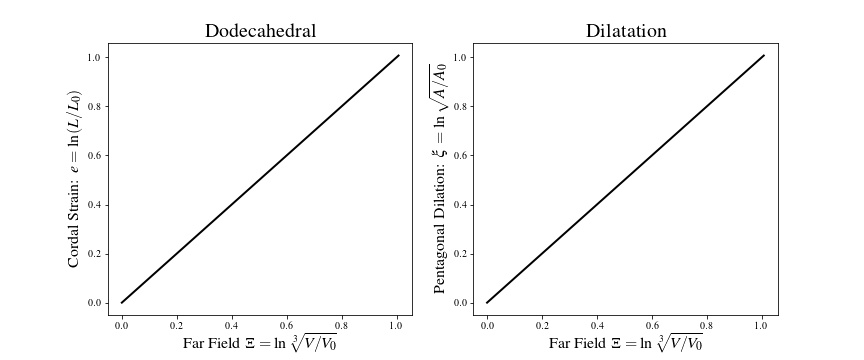
\includegraphics[width=\textwidth]{figures/dilatation.jpg}
	\caption{Response of a dodecahedron exposed to an isotropic motion of dilatation.  The abscissa is the control variable and the ordinates are response variables. The right graphic plots the areal response of the pentagons $\xi = \ln \sqrt{A / A_0}$, while the left graphic plots the axial response of the chords $e = \ln ( L / L_0)$. Both are plotted against the volumetric response of the dodecahedron $\Xi = \ln \sqrt[3]{V \! / V_0}$.  Here $V$ denotes dodecahedral volume, $A$ denotes pentagonal area, and $L$ denotes chordal length, all being evaluated in the current state, whose reference values are $V_0$, $A_0$ and $L_0$.}
	\label{figDilatation}
\end{figure}

\paragraph{Geometric vs.\ Thermodynamic Strains}

There are two types of strain measures that one can use to quantify deformation within a pentagon of a dodecahedron: geometric and thermo\-dynamic.  For the uniform far-field motion of volumetric expansion, only a thermo\-dynamic strain known as dilation, i.e., $\xi = \ln \sqrt{ab/a_0b_0}$, varies with the motion, and its response equals that of the geometric strain $\ln \sqrt{A / A_0}$, see Fig.~\ref{figDilatation2}.  Also present in this graph is an observation that the thermo\-dynamic strains for squeeze $\varepsilon$ and shear $\gamma$ do not contribute under motions of pure dilatation, as expected.  This further verifies the numerical implementation of our dodecahedral model.

\begin{figure}
	\centering
	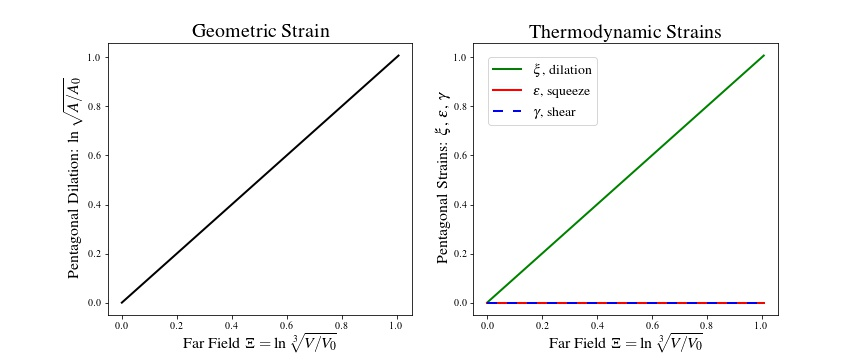
\includegraphics[width=\textwidth]{figures/dilatationGeoVsThermo.jpg}
	\caption{Response of a dodecahedron exposed to a far-field isotropic motion of dilatation.  The abscissa is the control variable and the ordinates are response variables. The right graphic plots the three thermo\-dynamic strains, as they apply to a pentagon, while the left graphic plots the geometric strain of a pentagon.}
	\label{figDilatation2}
\end{figure}

To put this into perspective, we compare with studies done by multiple investigators where ratios of alveolar surface area, viz., $A/A_0$, have been measured in rat, rabbit, guinea pig, and cat, cf.\ Roan and Waters \cite{RoanWaters11} (Table~1).  These experiments considered ranges that went as low as 25\% and as high as 100\% of total lung capacity.  Taking statistics of their tabulation produced results of $A/A_0 = 1.47 \pm 0.44$ during inflation and $A/A_0 = 1.18 \pm 0.14$ during deflation, which correspond to a $\xi = \ln\sqrt{A/A_0} = 0.19 \pm 0.18$ for inflation and a $\xi = \ln\sqrt{A/A_0} = 0.08 \pm 0.07$ for deflation.  These areal strain values coincide with chordal strains of $e=\ln(L/L_0) = 0.13$ measured \textit{in~vivo\/} around the periphery of an alveolus in rat lung, as reported by Perlman and Bhattachary \cite{PerlmanBhattacharya07}.  Our kinematics have been verified well past these physiologic ranges, viz., for dilatations up to 100\% logarithmic strain. 

\subsubsection{Isochoric Motions}

The motions of pure and simple shears are volume preserving.  Imposing these shears as far-field motions onto our dodecahedral model produced the results displayed in Fig.~\ref{figIsochoric}.  For a simple shear, the numerical model is in error by about machine precision, i.e., $\epsilon_m \approx 2.2 \times 10^{-16}$, for strains up to 100\%, while for pure shear (a special case of squeeze in 3D) the model is in error by about machine precision for strains up to of about 60\%, after which the error increases up to about $10\epsilon_m$ at strains around~100\%.  This further verifies the numerical implementation of our dodecahedral model.

\begin{figure}
	\centering
	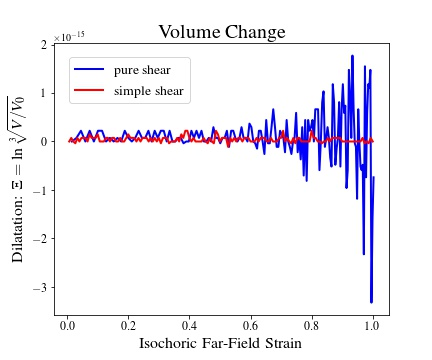
\includegraphics[width=10cm]{figures/isochoric.jpg}
	\caption{Response of a dodecahedron exposed to far-field motions of pure and simple shears.  Note that the ordinate is $\times 10^{-15}$ and machine precision is $\sim 2.2 \times 10^{-16}$.}
	\label{figIsochoric}
\end{figure}

\paragraph{Geometric Strains}

How the 30 chords and 12 irregular pentagons deform under far-field motions of pure shear is displayed in Fig.~\ref{figPureShears}.  Figure~\ref{figIsochoric} demonstrates that the overall response of a dodecahedron is isochoric during pure shear.  Regardless, Fig.~\ref{figPureShears} demonstrates that individual chordal and pentagonal constituents deform in a non-homogeneous manner, where the strains have been calculated as geometric changes in dodecahedral shape.  This result agrees with \textit{in~vivo\/} observations made by Perlman and Bhattacharya \cite{PerlmanBhattacharya07} where confocal microscopy was used to image a breathing rat lung.

\begin{figure}
	\centering
	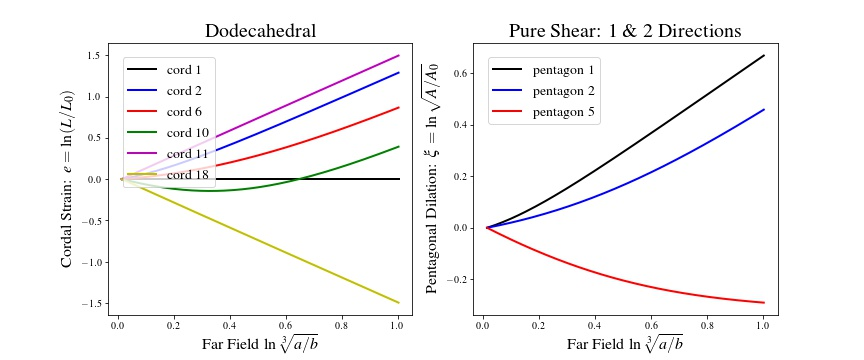
\includegraphics[width=\textwidth]{figures/squeeze12.jpg} \\
	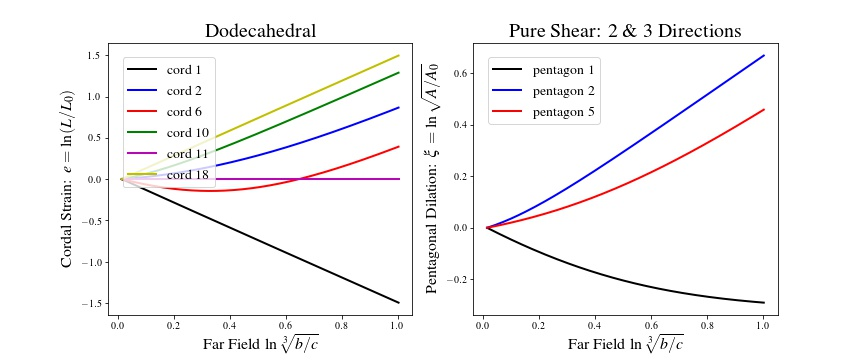
\includegraphics[width=\textwidth]{figures/squeeze23.jpg} \\
	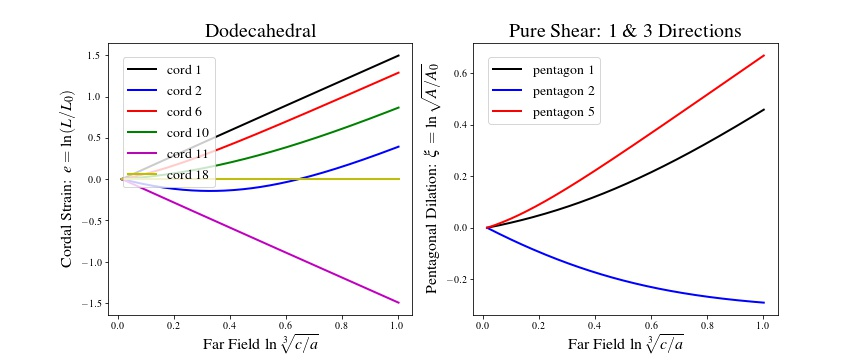
\includegraphics[width=\textwidth]{figures/squeeze13.jpg} 
	\caption{Response of a dodecahedron exposed to far-field pure-shear motions in the sense of Treloar \cite{Treloar75}: $a = \ell$, $b = 1/\ell$ and $c = 1$ in the top images; $a = 1$, $b = \ell$ and $c = 1/\ell$ in the middle images; and $a = 1/\ell$, $b = 1$ and $c = \ell$ in the bottom images, with $\ell$ denoting an elongation of extrusion.  In all six graphic images, the relevant (controlled) motion of the far-field pure shear is plotted along the abscissa.  In each image pair, the right graphic presents pentagonal dilations, while the left graphic presents chordal elongations. Only unique responses are plotted; repetitions are not.}
	\label{figPureShears}
\end{figure}

For the chords, there are six independent responses for dodecahedral motions of pure shear: two chords each for three of these lines, and eight chords each for the remaining three curves present in the left images of Fig.~\ref{figPureShears}.  For pentagons, there are three independent responses with four pentagons responding according to each curve shown in the right images.  Although different chords and pentagons deform differently when sheared in different directions, their collective responses are the same regardless of the far-field direction being sheared.  Consequently, the local geometric response of a dodecahedron is isotropic under the far-field motions of pure shear.  

How the 30 chords and 12 irregular pentagons deform under far-field motions of simple shear is displayed in Fig.~\ref{figSimpleShears}.  Figure~\ref{figIsochoric} demonstrates that the overall response of a dodecahedron is isochoric during a far-field simple shear. Figure~\ref{figSimpleShears} demonstrates that the individual chordal and pentagonal constituents deform in a non-homogeneous manner during simple shears, like they do for pure shears.  However, unlike pure shears whose collective chordal and pentagonal responses remain isotropic, here they diverge slightly from isotropy under motions of simple shear.  Simple shears in the 12 and 23 planes have the same collective response; whereas, simple shear in the 13 plane has a slightly different response with respect to changes in the shearing direction.  

\begin{figure}
	\centering
	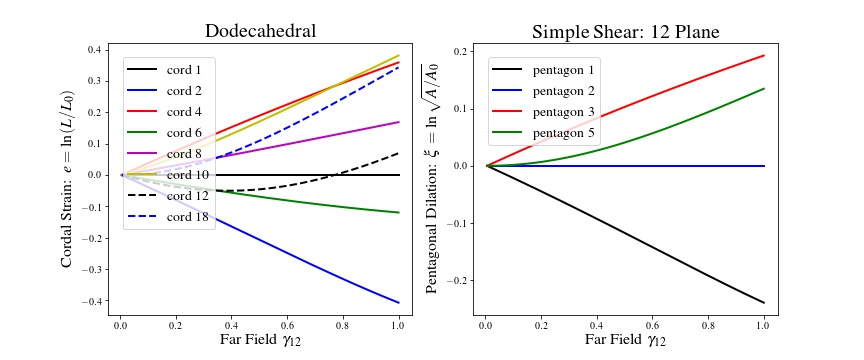
\includegraphics[width=\textwidth]{figures/shear12.jpg} \\
	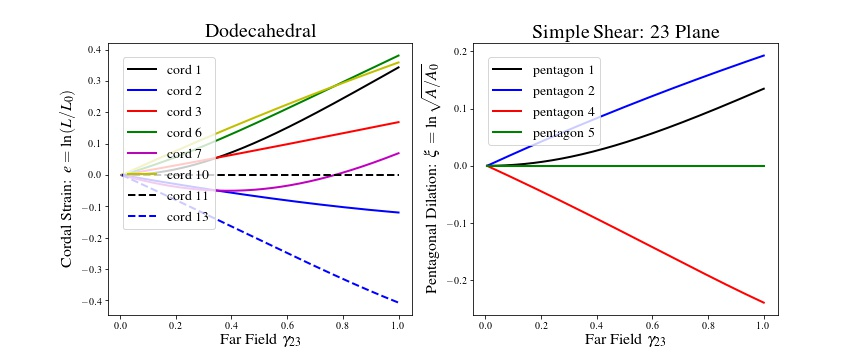
\includegraphics[width=\textwidth]{figures/shear23.jpg} \\
	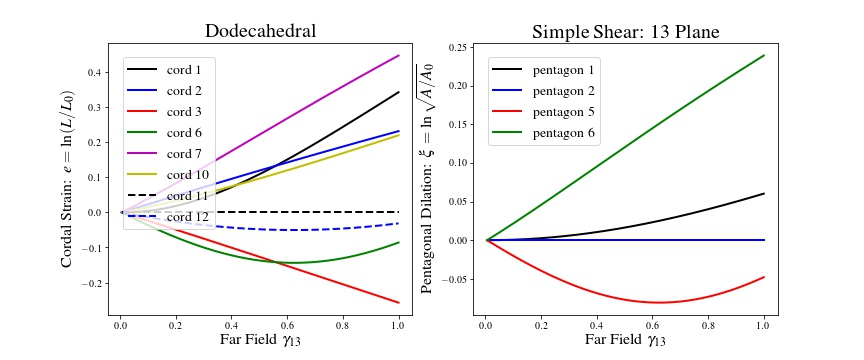
\includegraphics[width=\textwidth]{figures/shear13.jpg} 
	\caption{Response of a dodecahedron exposed to far-field simple-shear motions.  In all six graphic images, the relevant (controlled) motion of simple shear is plotted along the abscissa.  In each image pair, the right graphic presents pentagonal dilations, while the left graphic presents chordal elongations. Only unique responses are plotted; repetitions are not. Responses in the 13 plane differ slightly from those of the 12 and 23 planes.}
	\label{figSimpleShears}
\end{figure}

Figures \ref{figDilatation}--\ref{figSimpleShears} show that a dodecahedron is (nearly, but not completely) isotropic in its kinematic response, as measured by the geometric strains $e = \ln (L / L_0)$, $\xi = \ln \sqrt{A / A_0}$, and $\Xi = \ln \sqrt[3]{V / V_0}$.  Furthermore, even though a far-field deformation is homogeneous, in accordance with our Conjecture on pg.~\pageref{conjecture}, the local deformations within the individual constituents of an alveolus will typically be heterogeneous, which agrees with imaging data \cite{PerlmanBhattacharya07}.

\paragraph{Thermodynamic Strains}

Addressing the septal response, modeled here as a set of 12 irregular pentagons per alveolus, we desire to come to a determination regarding how to best model the deformation occurring within these alveolar septa.  In the section above we investigated the geometric response of alveolar septa via the strain measure $\ln \sqrt{A/A_0}$, which quantifies dilation.  

The thermo\-dynamic strains arising from a Gram--Schmidt factorization of the deformation gradient put forward in \S\ref{secQR} specify three strain measures pertinent to a membrane: dilation $\xi = \ln \sqrt{ab/a_0 b_0}$, squeeze $\varepsilon = \ln \sqrt{ab_0 / a_0 b}$, and shear $\gamma = g - g_0$, where elongations $a$ and $b$ and magnitude of shear $g$ are illustrated in Fig.~\ref{figKinematics}.  Of these, dilation is an uniform response, while squeeze and shear describe isochoric non-uniform responses.  To acquire them requires knowing the deformation gradient.

The curves in Figs.~\ref{figPureShears} and \ref{figSimpleShears} were obtained from geometric measures for chordal strain $\ln (L/L_0)$ and areal dilation $\ln \sqrt{A/A_0}$.  They were computed under separate far-field conditions of pure and simple shears.  The curves in Figs.~\ref{figPureShearsPentagons} and \ref{figSimpleShearsPentagons} were obtained from thermo\-dynamic measures for membrane strain under the same far-field deformations.  The strains of dilation $\xi$, squeeze $\varepsilon$, and shear $\gamma$ were computed in accordance with \S\ref{secQR} using deformation gradients gotten from the pentagonal shape functions of Wachspress \cite{Wachspress75} discussed in \S\ref{secShapeFns}.\footnote{
	Five constant-strain triangles were also used to quantify the deformation gradient for each pentagonal surface at its centroid---the common vertex to all five triangles.  This approach provided accurate descriptions for uniform strain, i.e., dilation $\xi$, but not for the two non-uniform strains, viz., squeeze $\varepsilon$ and shear $\gamma$; hence, our preference to use Wachspress shape functions for alveolar planes.
} 

\begin{figure}
	\centering
	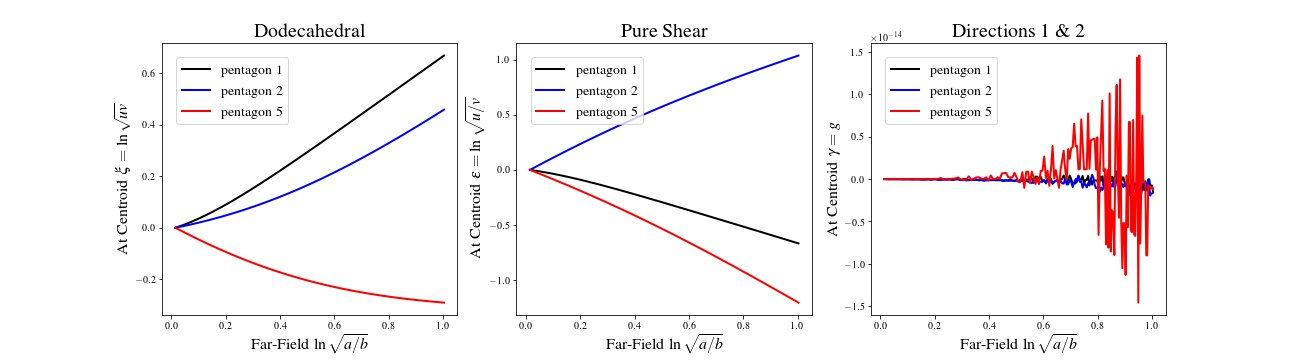
\includegraphics[width=\textwidth]{figures/pentagonalPureShear12.jpg} \\
	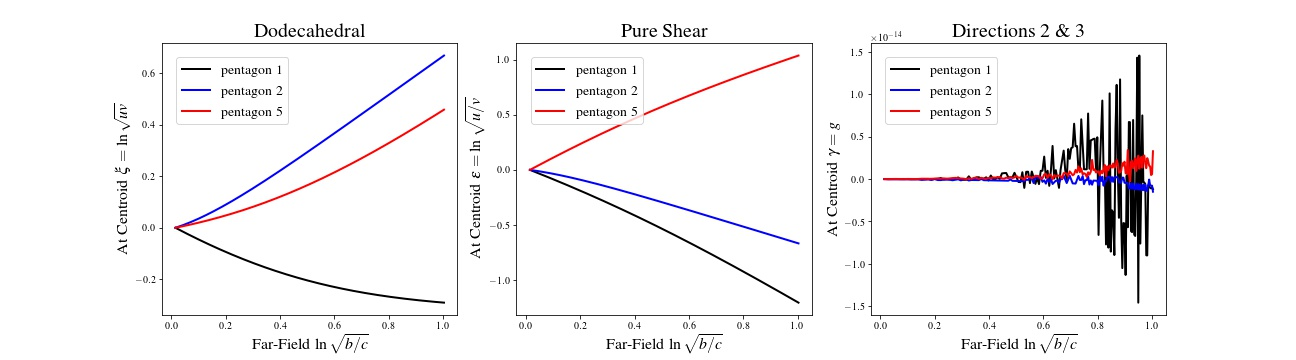
\includegraphics[width=\textwidth]{figures/pentagonalPureShear23.jpg} \\
	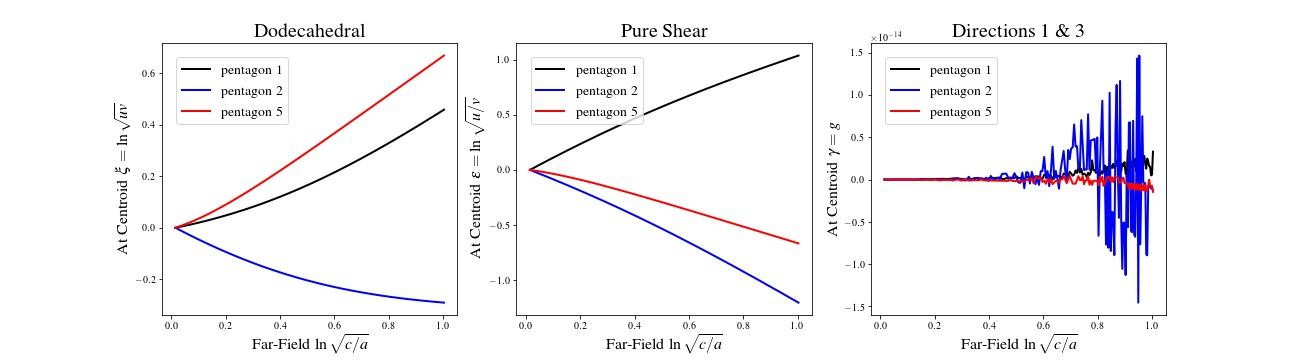
\includegraphics[width=\textwidth]{figures/pentagonalPureShear13.jpg} \\
	\caption{Same boundary conditions as in Fig.~\ref{figPureShears}.  Pentagonal areas were used to compute dilation in Fig.~\ref{figPureShears}.  The shape functions of Wachspress were used to compute dilation here.  The uniform response in the right column of Fig.~\ref{figPureShears} and in the left column above are the same, providing additional assurance that the code has been correctly implemented.  The squeeze response shown in the center column is the same for all three orientations of far-field pure shear, i.e., this response is isotropic.  The right column has ordinates scaled by $10^{-14}$ implicating that there is no effective simple shear response occurring within any pentagonal surface of the dodecahedron whenever it is subjected to a far-field motion of pure shear.}
	\label{figPureShearsPentagons}
\end{figure}

\begin{figure}
	\centering
	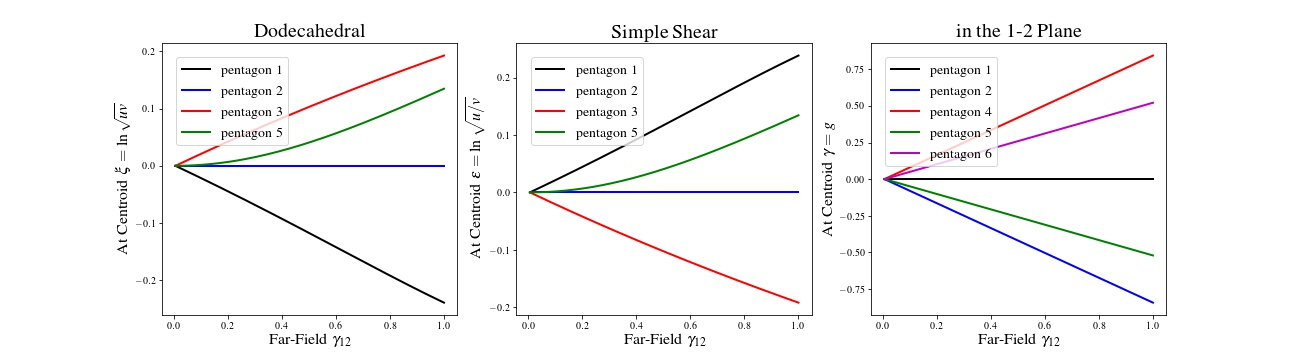
\includegraphics[width=\textwidth]{figures/pentagonalSimpleShear12.jpg} \\
	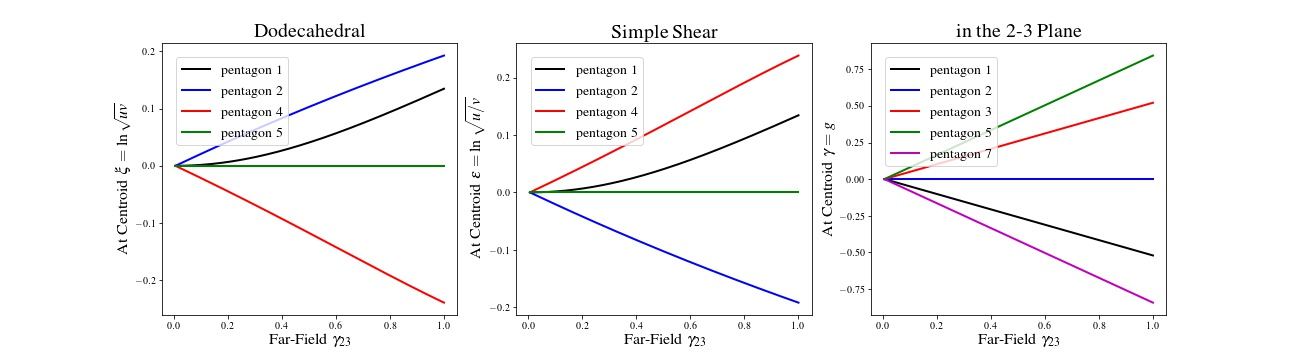
\includegraphics[width=\textwidth]{figures/pentagonalSimpleShear23.jpg} \\
	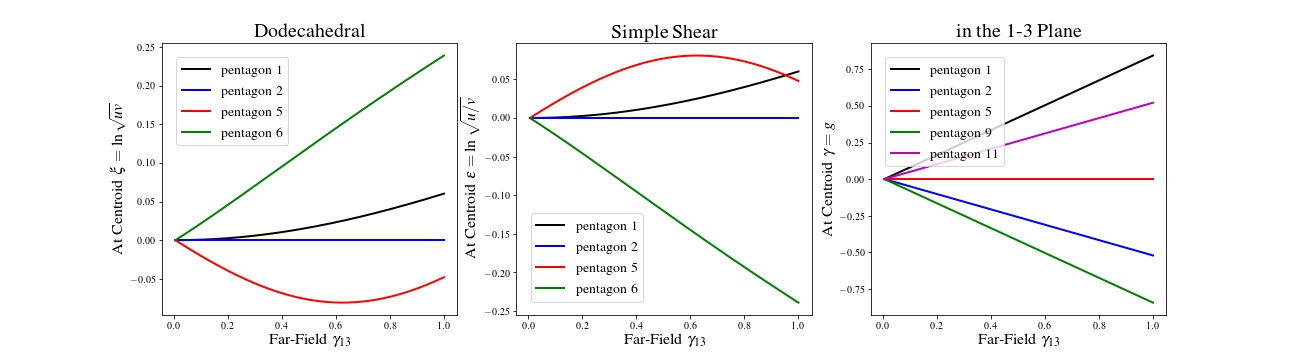
\includegraphics[width=\textwidth]{figures/pentagonalSimpleShear13.jpg} \\
	\caption{Same boundary conditions as in Fig.~\ref{figSimpleShears}.  Pentagonal areas were used to compute dilation in Fig.~\ref{figSimpleShears}.  The shape functions of Wachspress were used to compute dilation here. The uniform response in the right column of Fig.~\ref{figSimpleShears} and in the left column above are the same, providing additional assurance that the code has been correctly implemented.  Like the dilational responses of the left column, the squeeze responses of the center column are the same in the 12 and 23 planes, but differ in the 13 plane.  In all cases, the simple shear response of any pentagonal plane is proportional to that of the far-field shear imposed, further substantiating the code's implementation.  The shear response of the septal membranes is isotropic.}
	\label{figSimpleShearsPentagons}
\end{figure}

Figures~\ref{figPureShears}--\ref{figSimpleShearsPentagons} allow us to conclude that if septal dilation were the only mode of planar deformation thought to cause a mechanical response, then knowledge of the geometric strain $\xi = \ln \sqrt{A/A_0}$ would be adequate; there would be no need to introduce a separate finite element discretization of the septal planes for acquiring their deformation gradients.  However, if the non-uniform responses of squeeze $\varepsilon$ and shear $\gamma$ are thought to contribute to the overall mechanical response of these membranes, then the shape functions of Wachspress \cite{Wachspress75,Wachspress16} ought to be used for acquiring the deformation gradient within a septal plane.  We found, but do not present figures to support this observation, that constant-strain triangles are not accurate enough for our application whenever non-uniform deformations are considered.  Strains derived from Wachspress shape functions are inhomogeneous; consequently, the deformation gradient will need to be evaluated at each Gauss point of integration within a pentagon, cf.\ \S\ref{secPentagonGaussPts}.

\subsubsection{Co-ordinate Pivoting}

The pivoting strategy of \S\ref{secRemedy} used to address the physical dilemma of \S\ref{secDilemma} did not engage often during our assessment of the code, but it did arise at least twice with effects illustrated in Figs.~\ref{figPivoting1} and \ref{figPivoting3}.  Here one can see that there is a clear effect on the shear response within four pentagonal planes; however, no change is observed to have occurred in either the dilation or squeeze responses, as expected.  It is not always possible to know when or where a co-ordinate relabeling ought to occur; consequently, the algorithm put forward in \S\ref{secRemedy} is deemed necessary.

\begin{figure}
	\centering
	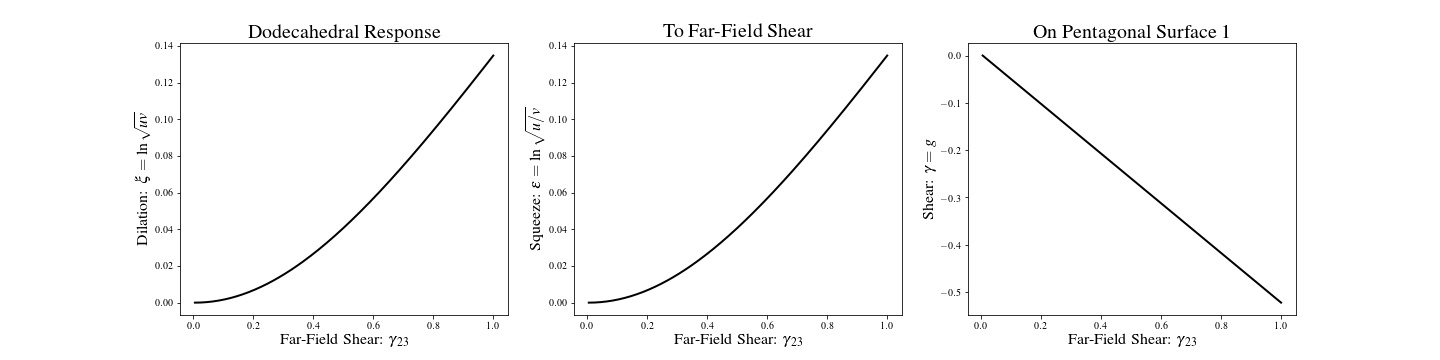
\includegraphics[width=\textwidth]{figures/continuousShearWithPivot1.jpg}
	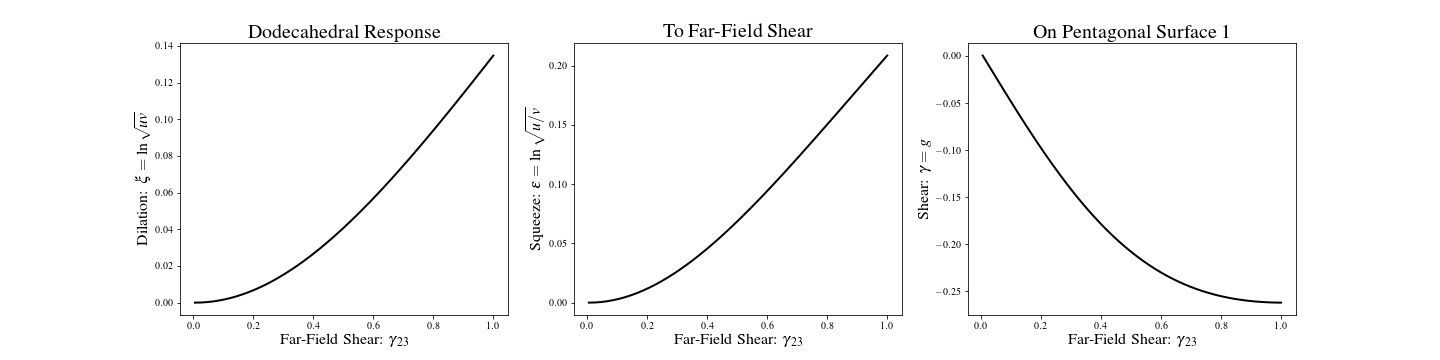
\includegraphics[width=\textwidth]{figures/continuousShearNoPivot1.jpg}
	\caption{A far-field shear of $\gamma_{23}$ is imposed on the dodecahedron.  Pentagons 1 and 8 exhibit the plotted response.  The top set of figures result whenever the pivoting strategy of \S\ref{secRemedy} is used, while the bottom set of figures result whenever no pivoting strategy is employed.  The dilation (left graphs) and squeeze (center graphs) responses are not effected by pivoting, only shear (right graphs) is effected.  Pivoting maintains a linear shear response under a far-field shearing of the dodecahedron, as desired.}
	\label{figPivoting1}
\end{figure}

\begin{figure}
	\centering
	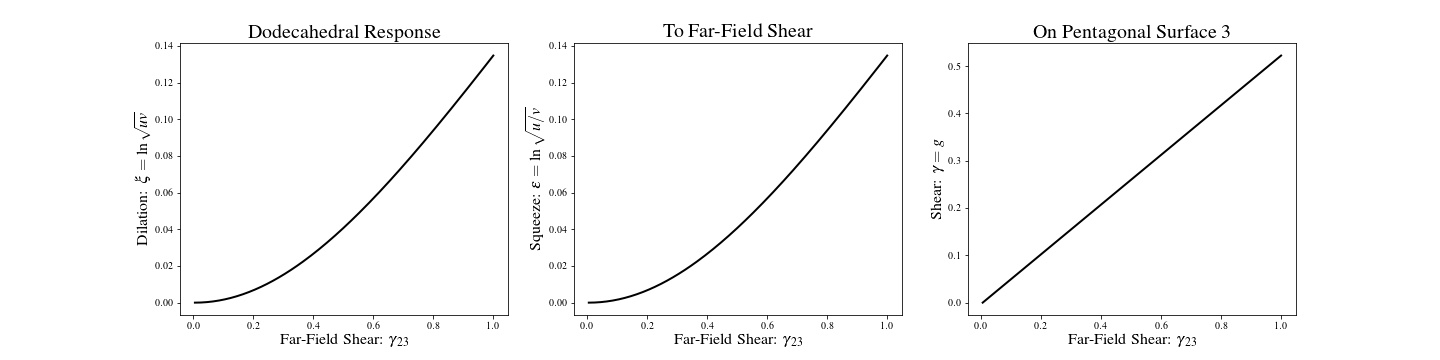
\includegraphics[width=\textwidth]{figures/continuousShearWithPivot3.jpg}
	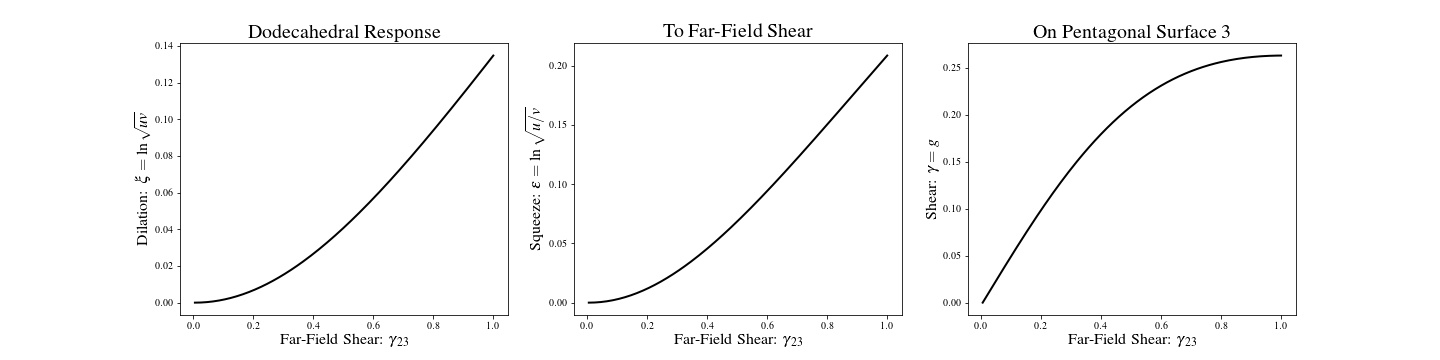
\includegraphics[width=\textwidth]{figures/continuousShearNoPivot3.jpg}
	\caption{A far-field shear of $\gamma_{23}$ is imposed on the dodecahedron.  Pentagons 3 and 10 exhibit the plotted response.  The top set of figures result whenever the pivoting strategy of \S\ref{secRemedy} is used, while the bottom set of figures result whenever no pivoting strategy is employed.  The dilation (left graphs) and squeeze (center graphs) responses are not effected by pivoting, only shear (right graphs) is effected.  Pivoting maintains a linear shear response under a far-field shearing of the dodecahedron, as desired.}
	\label{figPivoting3}
\end{figure}

\subsubsection{Compatible Membrane Deformations}

For a deformation to be compatible, and therefore integrable, the curl of its deformation gradient must vanish, viz., $\textrm{curl} (\mathbfsf{F}) = \textbf{0}$ \cite{Clayton15}. Equation~\ref{compatibility} provides constraint equations for the compatibility of planar motions, e.g., septal planes of an alveolus.  Here we test to make sure that these conditions are satisfied within the pentagonal planes of our alveolar dodecahedron, assuming that the shape functions of Wachspress apply.

Figure \ref{figCompatDilatation} presents the compatibility response at the centroid of a typical pentagonal plane during the uniform expansion of a regular dodecahedron out to 100\% strain.   Theoretically, all four derivatives should be zero for this motion. Actually, their values are on the order of machine precision.  Most importantly, whenever they are not zero, they lie along the $45^{\circ}$ diagonal, thereby verifying compatibility in the case of a dilatation.

\begin{figure}
	\centering
	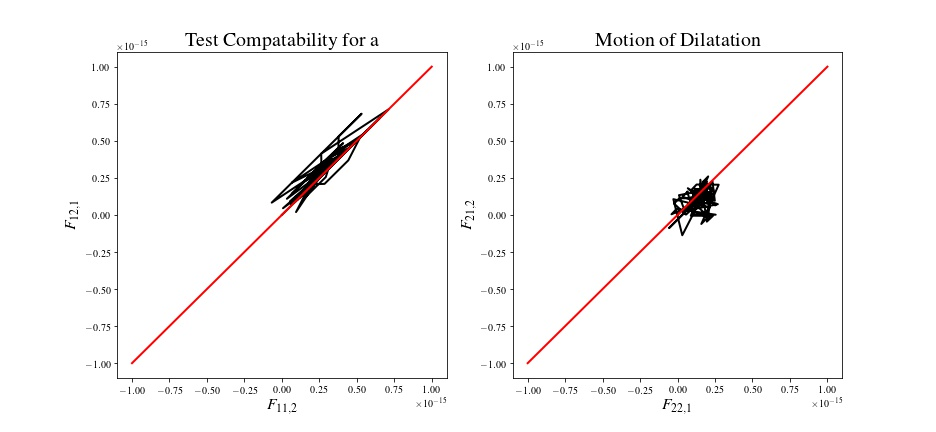
\includegraphics[width=\textwidth]{figures/compatibilityDilatation.jpg}
	\caption{Planar compatibility requires $F_{11,2} = F_{12,1}$ and $F_{22,1} = F_{21,2}$ where the left-hand sides of these formul\ae\ are plotted as the absciss\ae\ and the right-hand sides are plotted as the ordinates.  For compatibility, the response ought to lie along the $45^{\circ}$ diagonal, which is drawn in red over the range of $\pm 10^{-15}$ where machine precision is about $2.2 \times 10^{-16}$.  Here the motion is one of uniform dilatation out to 100\% strain.}
	\label{figCompatDilatation}
\end{figure}

Similarly, Figs.~\ref{figCompatPureShearP5} and \ref{figCompatSimpleShearP5} present typical responses for testing compatibility during far-field pure shear (Fig.~\ref{figCompatPureShearP5}) and simple shear (Fig.~\ref{figCompatSimpleShearP5}) deformations.  In both cases, one of the four pentagons around the girth of the dodecahedron (viz., \#5) has been selected, as both modes of deformation are activated in this pentagon.  In both cases, errors are typically less than 10 times machine precision, thereby verifying compatibility in the cases of squeeze and shear.

\begin{figure}
	\centering
	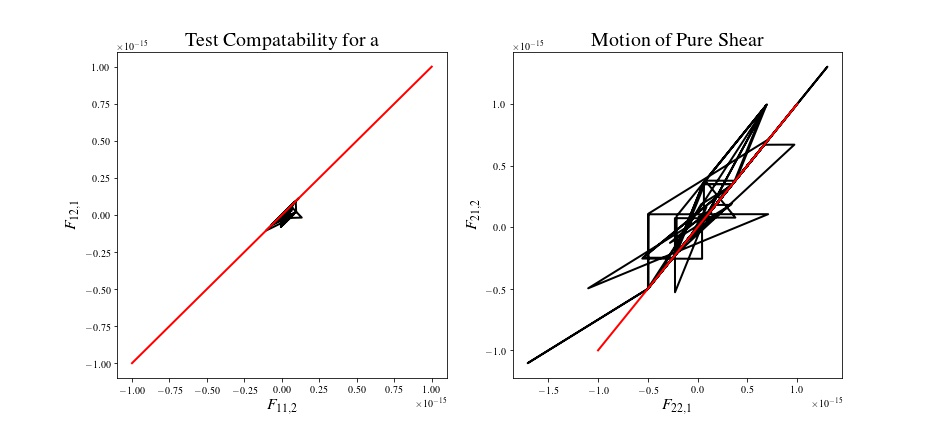
\includegraphics[width=\textwidth]{figures/compatibilityPureShearP5G7.jpg}
	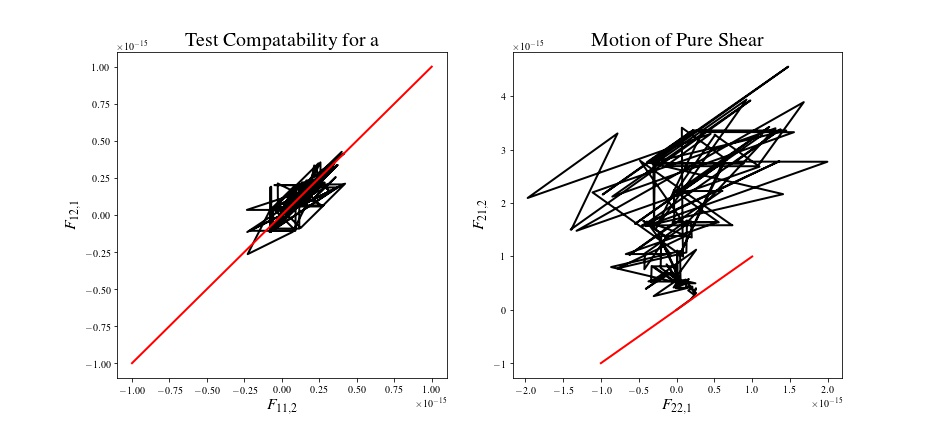
\includegraphics[width=\textwidth]{figures/compatibilityPureShearP5G5.jpg}
	\caption{Planar compatibility requires $F_{11,2} = F_{12,1}$ and $F_{22,1} = F_{21,2}$ where the left-hand sides of these formul\ae\ are plotted as the absciss\ae\ and the right-hand sides are plotted as the ordinates.  For compatibility, the response ought to lie along the $45^{\circ}$ diagonal, which is drawn in red over the range of $\pm 10^{-15}$ where machine precision is about $2.2 \times 10^{-16}$.  Here the motion is one of pure shear out to 100\% strain with elongation occurring in the 1-direction, contraction occurring in the 2-direction, while the 3-direction is held fixed.  These results pertain to pentagon~5: nodes 15, 5, 12, 11, 1, cf.\ Fig.~\ref{figDodecahedron} and Table~\ref{TablePentagons}.  The top row of figures is the best response among the Gauss points, while the bottom row of figures is the worst response.}
	\label{figCompatPureShearP5}
\end{figure}

\begin{figure}
	\centering
	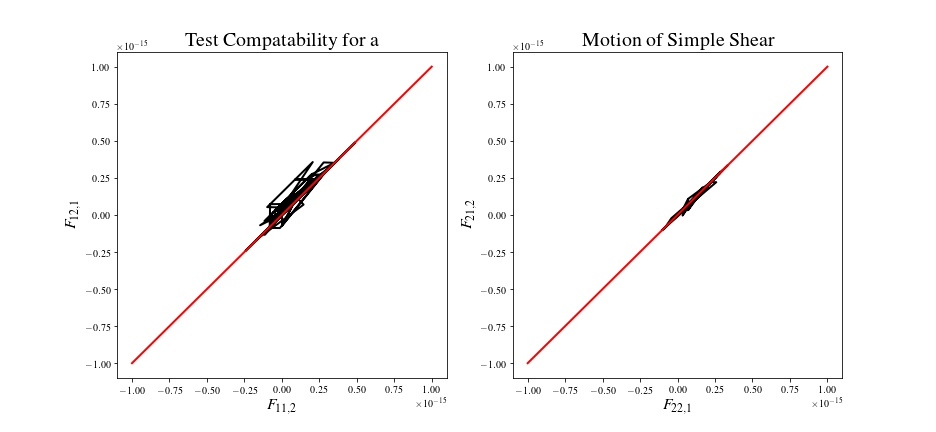
\includegraphics[width=\textwidth]{figures/compatibilitySimpleShearP5G7.jpg}
	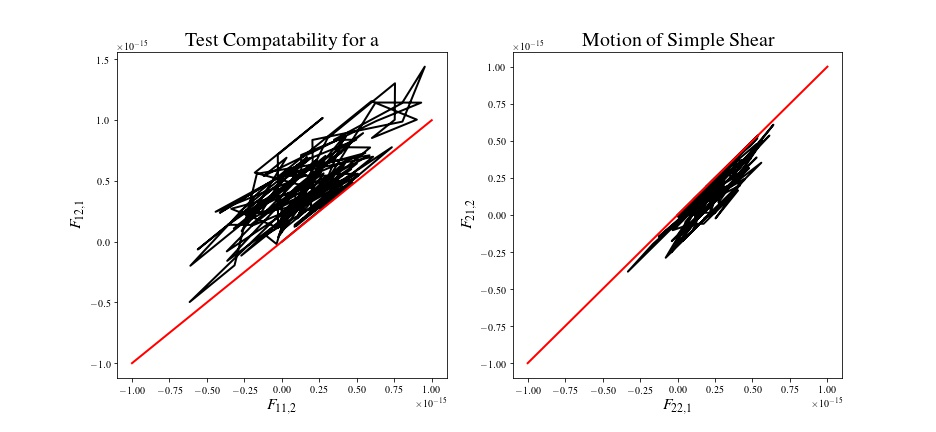
\includegraphics[width=\textwidth]{figures/compatibilitySimpleShearP5G5.jpg}
	\caption{Planar compatibility requires $F_{11,2} = F_{12,1}$ and $F_{22,1} = F_{21,2}$ where the left-hand sides of these formul\ae\ are plotted as the absciss\ae\ and the right-hand sides are plotted as the ordinates.  For compatibility, the response ought to lie along the $45^{\circ}$ diagonal, which is drawn in red over the range of $\pm 10^{-15}$ where machine precision is about $2.2 \times 10^{-16}$.  Here the motion is one of simple shear out to 100\% strain, shearing along 1-2~planes in the 1-direction.  These results pertain to pentagon~5: nodes 15, 5, 12, 11, 1, cf.\ Fig.~\ref{figDodecahedron} and Table~\ref{TablePentagons}.  The top row of figures is the best response among the Gauss points, while the bottom row of figures is the worst response.}
	\label{figCompatSimpleShearP5}
\end{figure}

This collective set of graphs, Figs.~\ref{figCompatDilatation}--\ref{figCompatSimpleShearP5}, investigate the constraint of compatibility in terms of the three fundamental modes of deformation: dilatation, squeeze, and shear.  These figures verify that the constraint of compatibility is satisfied when using the pentagonal shape functions of Wachspress \cite{Wachspress75,Wachspress16} in our dodecahedral model, as errors are typically less than 10 times machine precision.  This has been verified out to deformations that are at least 3 times those of their normal physiologic range.

\textit{Our kinematic analysis of a dodecahedron has been verified, both theoretically and numerically.}


%\setcounter{equation}{0}
%\setcounter{figure}{0}
%\setcounter{section}{0}
%\setcounter{table}{0}
\part{Constitutive Theory}
\label{partConstitutive}

Roan \& Waters \cite{RoanWaters11} and Suki \textit{et~al}.\ \cite{Sukietal05,Sukietal11} have each written extensive review articles on the mechanics of parenchyma, have provided detailed information about the structural constituents of alveoli, and have discussed their influence on the overall mechanical response of parenchyma.  Of particular importance, from a mechanics perspective, are the constituent building blocks of alveolar tissue: collagen (types I and III, predominantly), elastin, proteoglycans and other proteins, surfactant and cells (epithelial and endothelial, predominantly).  These constituents are assembled in such a manner so as to produce a variety of alveolar sub-structures that are essentially 1D (alveolar chords), 2D (alveolar septa) and 3D (alveolar sacs) in their geometric construction.

A dodecahedron is used here as a geometric model for an alveolus \cite{FrankusLee74}, cf.\ Figs.~\ref{figRatLung} \& \ref{figDodecahedron}.  It is comprised of: thirty 1D rods that represent alvolar chords, twelve 2D membranes that represent alveolar septa, considered here to be pentagonal in shape, and one 3D cavity filled with air (or fluids in the case of a contusion caused by injury or an edema caused by disease), considered here to be dodecahedral in shape.  The thermo\-elastic constitutive equations presented in this chapter for these three spatial geometries are derived in \ref{appImplicitElasticity}.  Elastic behavior is sufficient for our intended application of studying alveoli being subjected to traveling waves.

We recall from our kinematic study of a dodecahedron that the geometric strains of $e \defeq \ln ( L / L_0 )$ for the elongation of septal chords, $\xi \defeq \ln \sqrt{A / A_0}$ for the dilation of septal membranes, and $\Xi \defeq \ln \sqrt[3]{V / V_0}$ for the dilatation of alveolar volume are equivalent to one another under motions of uniform expansion.  These three, geometric, strain measures also exist as thermo\-dynamic strains, each associating with a distinct and unique conjugate stress.

Constitutive equations are a derived consequence from physical laws governing thermo\-dynamic processes.  Here we derive constitutive equations applicable for 1D thermo\-elastic fibers (alveolar chords), 2D thermo\-elastic membranes (alveolar septa), and 3D thermo\-elastic volumes (alveolar sacs).  In \S\ref{secUniformCE}, we assume that the motions are uniform in their spatial dimension.  Later, in \S\ref{secNonuniform2D}, the non-uniform motions of shears associated with a membrane are included into this thermo\-dynamic framework.  Section~\ref{secAlveolus} pulls these results together, sufficient for the intended purpose of modeling the three structural facets that comprise an alveolous.  Specifically, all geometric entities (alveolar chords, alveolar septa, and alveolar sacs) are described in terms of stresses ($\text{dyne/cm}^2$) instead of their intensive thermo\-dynamic forces (force, surface tension, and stress).  This is done to facilitate implementation of these models into code, and to facilitate interpretations of their results by engineers and scientists.

\section{Green Thermoelastic Solids Subjected to Uniform Motions in 1D, 2D \& 3D}
\label{secUniformCE}

Combining the First and Second Laws of Thermo\-dynamics governing uniform, reversible, adiabatic processes results in the following three formul\ae, one per dimension; they are
\begin{subequations}
    \label{thermoelasticLaws}
    \begin{align}
    \mbox{} & \text{In 1 Dimension:} & 
    \mathrm{d}\mathcal{U} & = \theta \, \mathrm{d} \eta +
    \tfrac{1}{\rho_{1D}} F \, \mathrm{d}L / L
    \label{thermoelastic1Dlaw} \\
    \mbox{} & \text{In 2 Dimensions:} &
    \mathrm{d}\mathcal{U} & = \theta \, \mathrm{d} \eta + 
    \tfrac{1}{\rho_{2D}} T \, \mathrm{d}A / \! A
    \label{thermoelastic2Dlaw} \\
    \mbox{} & \text{In 3 Dimensions:} &
    \mathrm{d}\mathcal{U} & = \theta \, \mathrm{d} \eta - 
    \tfrac{1}{\rho_{3D}} P \, \mathrm{d}V \! / V \!
    \label{thermoelastic3Dlaw}
    \end{align}
\end{subequations}
wherein $\mathcal{U}$ is an internal energy density (erg/gr = dyne.cm/gr), which is a function of state, $\theta$ is a temperature in Kelvin ($273 + \mbox{}^{\circ}$C), $\eta$ is an entropy density (erg/gr.K), $L$ is a length of line (cm), $A$ is an area of surface ($\text{cm}^2$), $V$ is a volume in space ($\text{cm}^3$), $F$ is a force (dyne), $T$ is a surface tension (dyne/cm), and $P$ is a pressure (dyne/$\text{cm}^2$ = barye), whereas the mass densities $\rho_{1D}$ ($\text{gr/cm}$), $\rho_{2D}$ ($\text{gr/cm}^2$) and $\rho_{3D}$ ($\text{gr/cm}^3$) associate with a reference state of per unit length, or per unit area, or per unit volume, as appropriate.  Pressure $P$ is assigned to be positive whenever a body undergoes hydro\-static compression, per accepted practice.

\subsection{Constitutive Equations}

Because the internal energy density $\mathcal{U}$ is a state function, its total derivative describes a Pfaffian form \cite{Caratheodory09} out of which the following constitutive formul\ae\ are readily obtained
\begin{subequations}
    \label{GreenElasticCEs}
    \begin{align}
    \mbox{} & \text{In 1 Dimension:} & 
    \theta & = \partial_{\eta\,} \mathcal{U} ( \eta , e) &
    F & = \rho_{1D} \, \partial_{e\,} \mathcal{U} ( \eta , e) \\
    \mbox{} & \text{In 2 Dimensions:} &
    \theta & = \partial_{\eta\,} \mathcal{U} ( \eta , \xi) &
    2T & = \rho_{2D} \, \partial_{\xi\,} \mathcal{U} ( \eta , \xi) \\
    \mbox{} & \text{In 3 Dimensions:} &
    \theta & = \partial_{\eta\,} \mathcal{U} ( \eta ,  \Xi) &
    -3P & = \rho_{3D} \, \partial_{\Xi\,} \mathcal{U} ( \eta ,  \Xi)
    \end{align}
\end{subequations}
where we have used the geometric strain definitions $e \defeq \ln ( L / L_0 )$, $\xi \defeq \ln \sqrt{ A / \! A_0 }$ and $\Xi \defeq \sqrt[3]{V \! / V_0}$, in accordance with Part~\ref{partKinematics}. These constitutive equations govern Green thermo\-elastic solids undergoing uniform motions in adiabatic enclosures.  As a convenience, we employ the following notation $\partial_{\eta\,} \mathcal{U} \defeq \partial \mathcal{U} / \partial \eta$, etc.

Consider the response variables for temperature and force\slash surface-tension\slash pressure to be $C^1$ functions of state (cf.\ Weinhold \cite{Weinhold75c} and Gilmore \cite{Gilmore84}) in a Green thermo\-elastic solid undergoing an uniform adiabatic motion.  One can then differentiate Eqn.~(\ref{GreenElasticCEs}), thereby producing the following collection of coupled differential equations
\begin{subequations}
    \label{GreenElasticODEs}
    \begin{align}
    \mbox{} & \text{In 1 Dimension:} &
    \left\{ \begin{matrix} \mathrm{d} \theta \\ 
    \mathrm{d} F \end{matrix} \right\} & = \begin{bmatrix}
    \partial_{\eta\eta\,} \mathcal{U} & \partial_{\eta e\,} \mathcal{U} \\
    \rho_{1D} \, \partial_{e\eta\,} \mathcal{U} & \rho_{1D} \, \partial_{ee\,} \mathcal{U} \end{bmatrix} 
    \left\{ \begin{matrix} \mathrm{d} \eta \\
    \mathrm{d} e \end{matrix} \right\} \\
    % second formula
    \mbox{} & \text{In 2 Dimensions:} &
    \left\{ \begin{matrix} \mathrm{d} \theta \\ 
    2 \, \mathrm{d} T \end{matrix} \right\} & = \begin{bmatrix}
    \partial_{\eta\eta\,} \mathcal{U} & \partial_{\eta \xi\,} \mathcal{U} \\
    \rho_{2D} \, \partial_{\xi\eta\,} \mathcal{U} & \rho_{2D} \, \partial_{\xi\xi\,} \mathcal{U} \end{bmatrix} \left\{ \begin{matrix} \mathrm{d} \eta \\
    \mathrm{d} \xi \end{matrix} \right\} \label{GreenMembrane} \\
    % third formula
    \mbox{} & \text{In 3 Dimensions:} &
    \left\{ \begin{matrix} \mathrm{d} \theta \\ 
    -3 \, \mathrm{d} P \end{matrix} \right\} & = \begin{bmatrix}
    \partial_{\eta\eta\,} \mathcal{U} & \partial_{\eta \Xi\,} \mathcal{U} \\
    \rho_{3D} \, \partial_{\Xi\eta\,} \mathcal{U} & \rho_{3D} \, \partial_{\Xi\Xi\,} \mathcal{U} \end{bmatrix} \left\{ \begin{matrix} \mathrm{d} \eta \\
    \mathrm{d} \Xi \end{matrix} \right\}
    \end{align}
\end{subequations}
where, from calculus, mixed partial derivatives obey $\partial_{e\eta\,} \mathcal{U} = \partial^2 \mathcal{U} / \partial e \partial \eta = \partial^2 \mathcal{U} / \partial \eta \partial e = \partial_{\eta e\,} \mathcal{U}$, etc., that in the thermo\-dynamics literature are known as Maxwell's relations.

Changing cause and effect between entropy and temperature in Eqn.~(\ref{GreenElasticODEs}) leads to
\begin{subequations}
    \label{HelmholtzElasticODEs}
    \begin{align}
    \left\{ \begin{matrix} \mathrm{d} \eta \\ 
    \mathrm{d} F \end{matrix} \right\} & = \begin{bmatrix}
    1/\partial_{\eta\eta\,} \mathcal{U} & -\partial_{\eta e\,} \mathcal{U} / 
    \partial_{\eta\eta\,} \mathcal{U} \\
    \rho_{1D} \, \partial_{e\eta\,} \mathcal{U} / \partial_{\eta\eta\,} \mathcal{U} & \rho_{1D} ( \partial_{ee\,} \mathcal{U} - \partial_{e\eta\,} \mathcal{U} \!\cdot\! \partial_{\eta e\,} \mathcal{U} / \partial_{\eta\eta\,} \mathcal{U} ) \end{bmatrix} 
    \left\{ \begin{matrix} \mathrm{d} \theta \\
    \mathrm{d} e \end{matrix} \right\} \\
    % second formula
    \left\{ \begin{matrix} \mathrm{d} \eta \\ 
    2 \, \mathrm{d} T \end{matrix} \right\} & = \begin{bmatrix}
    1/\partial_{\eta\eta\,} \mathcal{U} & -\partial_{\eta \xi\,} \mathcal{U} / \partial_{\eta\eta\,} \mathcal{U} \\
    \rho_{2D} \, \partial_{\xi\eta\,} \mathcal{U} / \partial_{\eta\eta\,} \mathcal{U} & \rho_{2D} ( \partial_{\xi\xi\,} \mathcal{U} - \partial_{\xi\eta\,} \mathcal{U} \!\cdot\! \partial_{\eta\xi\,} \mathcal{U} / \partial_{\eta\eta\,} \mathcal{U} ) \end{bmatrix} \left\{ \begin{matrix} \mathrm{d} \theta \\
    \mathrm{d} \xi \end{matrix} \right\} \label{HelmholtzMembrane} \\
    % thrid formula
    \left\{ \begin{matrix} \mathrm{d} \eta \\ 
    -3 \, \mathrm{d} P \end{matrix} \right\} & = \begin{bmatrix}
    1/\partial_{\eta\eta\,} \mathcal{U} & -\partial_{\eta \Xi\,} \mathcal{U} / \partial_{\eta\eta\,} \mathcal{U} \\
    \rho_{3D} \, \partial_{\Xi\eta\,} \mathcal{U} / \partial_{\eta\eta\,} \mathcal{U} & \rho_{3D} ( \partial_{\Xi\Xi\,} \mathcal{U} - \partial_{\Xi\eta\,} \mathcal{U} \!\cdot\! \partial_{\eta\Xi\,} \mathcal{U} / \partial_{\eta\eta\,} \mathcal{U} ) \end{bmatrix} \left\{ \begin{matrix} \mathrm{d} \theta \\
    \mathrm{d} \Xi \end{matrix} \right\}
    \end{align}
\end{subequations}
which are written above in a format that is more useful for our multi\-scale application.  In this process, a localization procedure pulls temperature and strain from the continuum scale down to the alveolar scale.  The alveolar entropy and stress are then determined via the above constitutive equations.  Afterwords, an homogenization procedure pushes the updated alveolar entropy and stress up to the continuum level.  We employ the independent variables of a Helmholtz free energy, but we do not adopt his potential, preferring to retain the internal energy potential to ensure a proper incorporation of Maxwell's constraint.  

Constitutive equations (\ref{GreenElasticODEs} \& \ref{HelmholtzElasticODEs}) take on the form of hypo-elastic material models \cite{Truesdell55}, which are ideal for numerical implementation whenever one uses numerical solution techniques like those presented in Part~\ref{partNumericalMethods}.

\subsection{Material Constants}

Experiments are performed for the purpose of characterizing material behavior.  In mechanics, we relate measured material constants to gradients and curvatures of thermo\-dynamic potentials out of which material models are created.  Experiments are typically done to quantify the following material constants, selected per a material's physical dimension:
\begin{subequations}
\label{materialConstants}
\begin{align}
C_f & \defeq \theta \, \partial_{\theta} \eta |_F & 
\alpha_f & \defeq L^{-1} \, \partial_{\theta} L |_F = 
\partial_{\theta} e |_F &
E_{\theta} & \defeq L \, \partial_L F |_{\theta} = 
\partial_e F |_{\theta} \\
C_t & \defeq \theta \, \partial_{\theta} \eta |_T & 
\alpha_t & \defeq A^{-1} \, \partial_{\theta} A |_T = 
2 \, \partial_{\theta} \xi |_T &
M_{\theta} & \defeq A \, \partial_A T |_{\theta} = 
\tfrac{1}{2} \, \partial_{\xi} T |_{\theta} \\
C_p & \defeq \theta \, \partial_{\theta} \eta |_P & 
\alpha_p & \defeq V^{-1} \, \partial_{\theta} V |_P = 
3 \, \partial_{\theta} \Xi |_P &
-K_{\theta} & \defeq V \, \partial_V P |_{\theta} = 
\tfrac{1}{3} \, \partial_{\Xi} P |_{\theta}
\end{align}
\end{subequations}
Herein, the various specific heats $C_f$, $C_t$, $C_p$ (erg/gr.K) are, essentially,  all equivalent as they are all defined per unit mass, insensitive to dimension.  Hereafter they will be denoted simply as $C$.  However, the various thermal expansions $\alpha_f$, $\alpha_t$, $\alpha_p$ (1/K) are all distinct, as they are each defined with respect to their physical dimension, viz., $\alpha_f \defeq L^{-1} \, \partial L / \partial \theta |_F$, $\alpha_t \defeq A^{-1} \, \partial A / \partial \theta |_T$ and $\alpha_p \defeq V^{-1} \, \partial V / \partial \theta |_P$.  Parameter $E_{\theta}$ is a modulus of extension (dyne), parameter $M_{\theta}$ is a modulus of dilation (dyne/cm), and parameter $K_{\theta}$ is a modulus of dilatation ($\mathrm{dyne/cm}^2$), a.k.a.\ the bulk modulus, with each modulus being measured at fixed temperature.  Shear moduli are discussed later in \S\ref{secNonuniform2D}.  The above material constants are gradients; they constitute tangents to their associated physical response curves.  Consequently, they need not be of constant value throughout state space, like a Hookean material supposes them to be.  This is an important characteristic for our application.  Here we employ the commonly used notation $\partial_{\theta} \eta |_F \defeq ( \partial \eta / \partial \theta ) |_F$, etc.

In terms of the material constants given in Eqn.~(\ref{materialConstants}), of which there are three per dimension, the internal energy density has the following three curvatures associated with it.  For 1D materials:
\begin{subequations}
    \label{internalEnergies}
    \begin{align}
    % for 1D materials
    \partial_{\eta\eta\,} \mathcal{U} & = 
    \frac{\rho_{1D}\theta}{\rho_{1D} C - E_{\theta} \alpha_f^2 \theta } \\
    \partial_{ee\,} \mathcal{U} & = \frac{C E_{\theta}}
    {\rho_{1D} C - E_{\theta} \alpha_f^2 \theta} \\
    \partial_{\eta e\,} \mathcal{U} \equiv \partial_{e \eta\,} \mathcal{U} & = 
    \frac{-E_{\theta} \alpha_f \theta}{\rho_{1D} C - E_{\theta} \alpha_f^2 \theta} \\
    \intertext{For 2D materials:}
    \partial_{\eta\eta\,} \mathcal{U} & = 
    \frac{\rho_{2D} \theta}{\rho_{2D} C - M_{\theta} \alpha_t^2 \theta} \\
    \partial_{\xi\xi\,} \mathcal{U} & = \frac{4 C M_{\theta}}
    {\rho_{2D} C - M_{\theta} \alpha_t^2 \theta} \\
    \partial_{\eta \xi\,} \mathcal{U} \equiv \partial_{\xi \eta\,} \mathcal{U} & = 
    \frac{-2M_{\theta} \alpha_t \theta}
    {\rho_{2D} C - M_{\theta} \alpha_t^2 \theta} \\
    \intertext{For 3D materials (cf.\ Weinhold \cite{Weinhold75c} and Gilmore \cite{Gilmore84}):}
    \partial_{\eta\eta\,} \mathcal{U} & = 
    \frac{\rho_{3D} \theta}{\rho_{3D} C - K_{\theta} \alpha_p^2 \theta} \\
    \partial_{\Xi\Xi\,} \mathcal{U} & = \frac{9 C K_{\theta}}
    {\rho_{3D} C - K_{\theta} \alpha_p^2 \theta} \\
    \partial_{\eta\Xi\,} \mathcal{U} \equiv 
    \partial_{\Xi\eta\,} \mathcal{U} & = 
    \frac{-3K_{\theta} \alpha_p \theta}{\rho_{3D} C - K_{\theta} \alpha_p^2 \theta}
    \end{align}
\end{subequations}
These materials constants are constrained by thermo\-dynamics in that
\begin{equation}
    \label{thermodynamicConstraints}
    0 < E_{\theta} < \frac{\rho_{1D} C}{\alpha_f^2 \, \theta} \qquad
    0 < M_{\theta} < \frac{\rho_{2D} C}{\alpha_t^2 \, \theta} \qquad
    0 < K_{\theta} < \frac{\rho_{3D} C}{\alpha_p^2 \, \theta}
\end{equation} 
which ensure that their respective thermo\-dynamic Jacobians cannot become singular. Singularities can and do occur, e.g., during a phase change in a crystal \cite{McLellan76,Gilmore84}, but such processes are not expected to arise in our application.

\subsection{Thermoelastic Models Suitable for Modeling Alveoli Subjected to Uniform Motions}

We now write down our constitutive formul\ae\ for quantifying uniform responses in thermo\-elastic solids of 1, 2 or 3 dimensions.  They are the thermo\-elastic constitutive equations (\ref{HelmholtzElasticODEs}) with Helmholtz variables expressed in terms of the material constants defined in Eqn.~(\ref{materialConstants}) assigned to the internal energy density $\mathcal{U}$ according to Eqn.~(\ref{internalEnergies}), with outcomes of
\begin{subequations}
    \label{HelmholtzCEs}
    \begin{align}\
    \text{For 1D Materials:} & &
    \left\{ \begin{matrix}
    \mathrm{d} \eta \\ \mathrm{d} F
    \end{matrix} \right\} & = \begin{bmatrix}
    C / \theta - E_{\theta} \alpha_f^2 / \rho_{1D}& 
    E_{\theta} \alpha_f / \rho_{1D} \\
    -E_{\theta} \alpha_f & E_{\theta}
    \end{bmatrix} \left\{ \begin{matrix}
    \mathrm{d} \theta \\ \mathrm{d} e
    \end{matrix} \right\} \label{Helmholtz1D} \\
    % the second equation
    \text{For 2D Materials:} & &
    \left\{ \begin{matrix}
    \mathrm{d} \eta \\ 2 \, \mathrm{d} T
    \end{matrix} \right\} & = \begin{bmatrix}
    C / \theta - M_{\theta} \alpha_t^2 / \rho_{2D} & 
    2 M_{\theta} \alpha_t / \rho_{2D} \\
    -2 M_{\theta} \alpha_t & 4 M_{\theta}
    \end{bmatrix} \left\{ \begin{matrix}
    \mathrm{d} \theta \\ \mathrm{d} \xi
    \end{matrix} \right\} \label{Helmholtz2D} \\
    % the third equation
    \text{For 3D Materials:} & &
    \left\{ \begin{matrix}
    \mathrm{d} \eta \\ -3 \, \mathrm{d} P
    \end{matrix} \right\} & = \begin{bmatrix}
    C / \theta - K_{\theta} \alpha_p^2 / \rho_{3D} & 
    3 K_{\theta} \alpha_p / \rho_{3D} \\
    -3K_{\theta} \alpha_p & 9 K_{\theta}
    \end{bmatrix} \left\{ \begin{matrix}
    \mathrm{d} \theta \\ \mathrm{d} \Xi
    \end{matrix} \right\} \label{Helmholtz3D}
    \end{align}
\end{subequations}
These constitutive formul\ae, derived from the First and Second Laws of Thermo\-dynamics, describe thermo\-elastic materials undergoing uniform motions through adibatic processes.

The whole upper-left component in each matrix of Eqn.~(\ref{HelmholtzCEs}) represents a specific heat evaluated at constant strain, divided by temperature---a material property not easily measured.  Whereas, the specific heat evaluated at constant pressure, viz., $C$, is more amenable to experiments, and is the property that one typically finds in published data tables.  

There are four material constants for each dimension (e.g., for 1D materials they are: $\rho_{1D}$, $C$, $\alpha_f$ and $E_{\theta}$) with the latter three being defined according to Eqn.~(\ref{materialConstants}).  The differential equations in Eqn.~(\ref{HelmholtzCEs}) have mathematical forms of hypo-elastic materials \cite{Truesdell55}, which are preferred for incorporating constitutive equations into finite element packages.

\section{Green Thermoelastic Membranes Subjected to Non-Uniform Motions}
\label{secNonuniform2D}

For modeling alveolar geometry via a dodecahedron, only the septal membranes are considered as  being capable of supporting shears, and therefore, only they need to have their constitutive structure extended to include the non-uniform motions of shear, of which pure shears (squeeze) are likely to dominate over simple shears.

The First and Second Laws of Thermo\-dynamics governing a reversible adiabatic process are described by the formula $\mathrm{d}\hspace{1pt}\mathcal{U} = \theta \, \mathrm{d} \eta + \tfrac{1}{\rho} \, \mathrm{d}W$, where $\mathrm{d}W$ is the mechanical power expended by stressing a body of mass density $\rho$.  For the case of a 2D planar membrane, a mass density of $\rho \Leftarrow \rho_{2D}$ applies, with its change in mechanical work being expressed as \cite{Freedetal17,FreedZamani19}
\begin{subequations}
\begin{align}
\mathrm{d} W & = \mathrm{tr} \left( 
\begin{bmatrix}
\mathcal{S}_{11} & \mathcal{S}_{12} \\
\mathcal{S}_{21} & \mathcal{S}_{22}
\end{bmatrix} \begin{bmatrix}
\mathrm{d}a / a & a \, \mathrm{d} g / b \\
0 & \mathrm{d}b / b 
\end{bmatrix} \right) =  
\pi \, \mathrm{d} \xi + \sigma \, \mathrm{d} \varepsilon + 
\tau \, \mathrm{d} \gamma
\label{convectedWorkRate} \\
\intertext{wherein the $\mathcal{S}_{ij}$ are components of a surface tension evaluated in the co-ordinate frame of a membrane.  (In \S\ref{secAlveolus} they will be converted into stress components.)  Therefore, the First and Second Laws result in an exact differential equation of the form}
\mathrm{d} \hspace{1pt} \mathcal{U} & = \theta \, \mathrm{d} \eta + \tfrac{1}{\rho_{2D}} 
\bigl( \pi \, \mathrm{d} \xi + \sigma \, \mathrm{d} \varepsilon + 
\tau \, \mathrm{d} \gamma \bigr)
\label{membraneThermo}
\end{align}
\end{subequations} 
where $\{ \pi , \sigma , \tau \}$ describes a set of intensive scalar-valued stresses whose thermo\-dynamic conjugates $\{ \xi , \varepsilon , \gamma \}$ describe a set of extensive scalar-valued strains.  (This contrasts with the classic approach where the work done is decomposed into a scalar-valued isotropic part and a tensor-valued deviatoric part.)  Pair $( \xi , \pi )$ describes a dilation $\xi$ caused by a surface tension $\pi$; it is the uniform contribution to stress power discussed in \S\ref{secUniformCE} where $2 \, \mathrm{d} \xi \Leftarrow A^{-1} \, \mathrm{d} A$ and $\tfrac{1}{2} \pi \Leftarrow T$.  Pair $( \varepsilon , \sigma )$ describes a pure shear $\varepsilon$ or squeeze caused by a normal-stress difference $\sigma$.  And pair $( \gamma , \tau )$ describes an in-plane shear $\gamma$ caused by a shear stress $\tau$. Collectively, pairs $( \varepsilon , \sigma )$ and $( \gamma , \tau )$ account for any non-uniform contributions to stress power, i.e., contributions from other than uniform dilations.  These pairs are quantified in \S\ref{secConjugatePairs}.

\subsection{Constitutive Equations}

Because a change in the internal energy $\mathrm{d} \hspace{1pt} \mathcal{U}$ governing a reversible adiabatic process is described by an exact differential \cite{Caratheodory09}, with $\mathcal{U}(\eta, \xi, \varepsilon, \gamma)$ in the case of a planar membrane, it follows that a constitutive response for a Green thermo\-elastic membrane is given by
\begin{subequations}
    \label{GreenThermoelasticity}
    \begin{align}
    \theta = \partial_{\eta\,} \mathcal{U}(\eta, \xi, \varepsilon, \gamma) , \;
    \pi & = \rho \, \partial_{\xi\,} \mathcal{U}(\eta, \xi, \varepsilon, \gamma) , \;
    \sigma = \rho \, \partial_{\varepsilon\,} \mathcal{U}(\eta, \xi, \varepsilon, \gamma) , \;
    \tau = \rho \, \partial_{\gamma\,} \mathcal{U}(\eta, \xi, \varepsilon, \gamma)
    \label{GreenThermoelasticMembrane} \\
    \intertext{with strain symmetries requiring that}
    \mathcal{U}(\eta, \xi, \varepsilon, \gamma) & =
    \mathcal{U}(\eta, \xi, -\varepsilon, \gamma) = 
    \mathcal{U}(\eta, \xi, \varepsilon, -\gamma) = 
    \mathcal{U}(\eta, \xi, -\varepsilon, -\gamma) .
    \label{internalEnergyInveriance}
    \end{align}
\end{subequations}
Considering that each intensive variable, viz., $\theta$, $\pi$, $\sigma$ and $\tau$, is actually a $C^1$ function of the set of extensive variables ($\eta , \xi , \varepsilon , \gamma$), then the constitutive expressions in Eqn.~(\ref{GreenThermoelasticMembrane}) can be recast into the following system of differential equations
\begin{equation}
\label{energies2D}
\left\{ \begin{matrix}
\mathrm{d} \theta \\ \mathrm{d} \pi \\
\mathrm{d} \sigma \\ \mathrm{d} \tau
\end{matrix} \right\} = \begin{bmatrix}
\partial_{\eta\eta\,} \mathcal{U} & 
\partial_{\eta\xi\,} \mathcal{U} & 
\partial_{\eta\varepsilon\,} \mathcal{U} & 
\partial_{\eta\gamma\,} \mathcal{U} \\ 
\rho \, \partial_{\xi\eta\,} \mathcal{U} & 
\rho \, \partial_{\xi\xi\,} \mathcal{U} & 
\rho \, \partial_{\xi\varepsilon\,} \mathcal{U} &
\rho \, \partial_{\xi\gamma\,} \mathcal{U} \\
\rho \, \partial_{\varepsilon\eta\,} \mathcal{U} & 
\rho \, \partial_{\varepsilon\xi\,} \mathcal{U} & 
\rho \, \partial_{\varepsilon\varepsilon\,} \mathcal{U} & 
\rho \, \partial_{\varepsilon\gamma\,} \mathcal{U} \\
\rho \, \partial_{\gamma\eta\,} \mathcal{U} & 
\rho \, \partial_{\gamma\xi\,} \mathcal{U} & 
\rho \, \partial_{\gamma\varepsilon\,} \mathcal{U} & 
\rho \, \partial_{\gamma\gamma\,} \mathcal{U} 
\end{bmatrix} 
\left\{ \begin{matrix}
\mathrm{d}\eta \\ \mathrm{d} \xi \\
\mathrm{d} \varepsilon \\ \mathrm{d} \gamma
\end{matrix} \right\}  
\end{equation}
whose upper-left $2\times 2$ sub-matrix also appears in Eqn.~(\ref{GreenMembrane}), which governs the uniform contribution of a response.  The above $4 \times 4$ matrix describes the full non-uniform response permissible by a Green thermo\-elastic membrane undergoing an adiabatic process.

For our application, it is reasonable to assume that the presence of a non-uniform planar motion will not cause an uniform planar response.  Said differently, it is reasonable to assume that pure $\varepsilon$ and simple $\gamma$ shears will not effect a change in either temperature $\theta$ or surface tension $\pi$.  Consequently, $\partial_{\eta\varepsilon\,} \mathcal{U} = \partial_{\eta\gamma\,} \mathcal{U} = \partial_{\xi\varepsilon\,} \mathcal{U} = \partial_{\xi\gamma\,} \mathcal{U} = 0$, and Eqn.~(\ref{energies2D}) simplifies to
\begin{displaymath}
\left\{ \begin{matrix}
\mathrm{d} \theta \\ \mathrm{d} \pi \\
\mathrm{d} \sigma \\ \mathrm{d} \tau
\end{matrix} \right\} = \begin{bmatrix}
\partial_{\eta\eta\,} \mathcal{U} & 
\partial_{\eta\xi\,} \mathcal{U} & 
0 & 0 \\ 
\rho \, \partial_{\xi\eta\,} \mathcal{U} & 
\rho \, \partial_{\xi\xi\,} \mathcal{U} & 
0 & 0 \\
0 & 0 & 
\rho \, \partial_{\varepsilon\varepsilon\,} \mathcal{U} & 
\rho \, \partial_{\varepsilon\gamma\,} \mathcal{U} \\
0 & 0 & 
\rho \, \partial_{\gamma\varepsilon\,} \mathcal{U} & 
\rho \, \partial_{\gamma\gamma\,} \mathcal{U} 
\end{bmatrix} 
\left\{ \begin{matrix}
\mathrm{d}\eta \\ \mathrm{d} \xi \\
\mathrm{d} \varepsilon \\ \mathrm{d} \gamma
\end{matrix} \right\} 
\end{displaymath}
with $\partial_{\varepsilon\eta\,} \mathcal{U} = \partial_{\gamma\eta\,} \mathcal{U} = \partial_{\varepsilon\xi\,} \mathcal{U} = \partial_{\gamma\xi\,} \mathcal{U} = 0$
because of Maxwell's relations.  Converting the above internal energy formulation into its Helmholtz equivalent results in
\begin{equation}
\left\{ \begin{matrix}
\mathrm{d} \eta \\ \mathrm{d} \pi \\
\mathrm{d} \sigma \\ \mathrm{d} \tau
\end{matrix} \right\} = \begin{bmatrix}
1 / \partial_{\eta\eta\,} \mathcal{U} & 
-\partial_{\eta\xi\,} \mathcal{U} / \partial_{\eta\eta\,} \mathcal{U} & 
0 & 0 \\ 
\rho \, \partial_{\xi\eta\,} \mathcal{U} / \partial_{\eta\eta\,} \mathcal{U} & 
\rho \bigl( \partial_{\xi\xi\,} \mathcal{U} - \partial_{\xi\eta\,} \mathcal{U} \!\cdot\! \partial_{\eta\xi\,} \mathcal{U} / \partial_{\eta\eta\,} \mathcal{U} \bigr) & 0 & 0 \\
0 & 0 & \rho \, \partial_{\varepsilon\varepsilon\,} \mathcal{U} & 
\rho \, \partial_{\varepsilon\gamma\,} \mathcal{U} \\
0 & 0 & \rho \, \partial_{\gamma\varepsilon\,} \mathcal{U} & 
\rho \, \partial_{\gamma\gamma\,} \mathcal{U} 
\end{bmatrix} 
\left\{ \begin{matrix}
\mathrm{d}\theta \\ \mathrm{d} \xi \\
\mathrm{d} \varepsilon \\ \mathrm{d} \gamma
\end{matrix} \right\}  
\label{Helmholtz2Duncoupled}
\end{equation}
which provides the general structure for a Green thermo\-elastic membrane appropriate for our application.  The uniform response (the upper-left $2 \times 2$ sub-matrix) and the non-uniform response (the lower-right $2 \times 2$ sub-matrix) are, by conjecture, decoupled in this constitutive construction.

\medskip\noindent
\textbf{Note}: There is experimental evidence that the bulk and shear moduli of parenchyma both depend upon transpulmonary pressure \cite{LaiFook79,Jahedetal90}.  It is conjectured that this is an alveolar structure effect, and that it is not a characteristic of the constituents which comprise an alveolus.  As such, we do not couple the uniform and non-uniform responses in Eqn.~(\ref{Helmholtz2Duncoupled}).

\subsection{Material Constants}
\label{secMaterialConstants}

The material model put forward here for a thermo\-elastic membrane has six material constants: a mass density $\rho$, a specific heat $C$, a coefficient for areal thermal expansion at constant surface tension $\alpha_{\pi}$, an areal modulus at constant temperature $M_{\theta}$ (2D version of a bulk modulus), a squeeze modulus at constant shear $N_{\gamma}$, and a shear modulus at constant squeeze $G_{\varepsilon}$.  The specific heat $C$ is defined as
\begin{subequations}
    \label{defineMaterialConstants}
    \begin{align}
    C & \defeq \theta \, \partial_{\theta} \eta |_{\mathcal{S}_{11} + \mathcal{S}_{22}} \! = \theta \, \partial_{\theta} \eta |_{\pi}
    \label{specificHeat2D} \\
    \intertext{where $\theta$ is temperature, $\eta$ is entropy, and $\pi =  \mathcal{S}_{11} + \mathcal{S}_{22} = 2T$ is the surface tension in a membrane, while $C$ is commonly referred to in the literature as the specific heat at constant pressure.  The areal coefficient for thermal expansion $\alpha_{\pi} = \alpha_t$ is defined as}
    \alpha_{\pi} & \defeq A^{-1} \, \partial_{\theta} A |_{\mathcal{S}_{11} + \mathcal{S}_{22}} \! = 2 \, \partial_{\theta} \xi |_{\pi}
    \label{thermalExpansionCoef2D} \\
    \intertext{where $A = ab$ is area and $\xi = \ln \sqrt{A / \! A_0}$ is dilation.  The areal modulus $M_{\theta}$ is defined as}
    M_{\theta} & \defeq A \, \partial_A \tfrac{1}{2} (\mathcal{S}_{11} + \mathcal{S}_{22}) |_{\theta} = \tfrac{1}{4} \, \partial_{\xi} \pi |_{\theta} .
    \label{arealCompliance2D} \\
    \intertext{The in-plane squeeze modulus $N_{\gamma}$ is defined as}
    N_{\gamma} & \defeq \Gamma \, \partial_{\Gamma} (\mathcal{S}_{11} - \mathcal{S}_{22}) |_g = \tfrac{1}{2} \, \partial_{\varepsilon} \pi |_{\gamma} 
    \label{arealSqueezeCompliance2D} \\
    \intertext{where $\sigma = \mathcal{S}_{11} - \mathcal{S}_{22}$ is a normal-stress difference, and $\Gamma = a/b$ is the stretch of squeeze with $\varepsilon = \ln \sqrt{\Gamma \! / \Gamma_0}$ being the strain of squeeze.  Finally, the in-plane shear modulus $G_{\varepsilon}$ is defined as}
    G_{\varepsilon} & \defeq \Gamma \, \partial_{g\,} \mathcal{S}_{21} |_{\Gamma} = \partial_{\gamma} \tau |_{\varepsilon} 
    \label{arealShearModulus2D}
    \end{align}
\end{subequations}
where $\tau = \Gamma \mathcal{S}_{21}$ determines the shear stress with $\gamma = g - g_0$ being the shear strain.  

Because $\ln (L/L_0) = \ln \sqrt{A / \! A_0}$ for uniform dilation (see Part~\ref{partKinematics}), it necessarily follows then that if an axial coefficient for thermal expansion $\alpha_{1D}$ is available, viz., $\alpha_{1D} = L^{-1} \, \partial_{\theta} L |_F$, then set $\alpha_{\pi} = 2 \alpha_{1D}$.  Furthermore, because $\ln \sqrt[3]{V \! / V_0} = \ln \sqrt{A / \! A_0}$ under uniform dilatation, it also follows that if a volumetric coefficient for thermal expansion $\alpha_{3D}$ is available, viz., $\alpha_{3D} = V^{-1} \, \partial_{\theta} V |_P$, then set $\alpha_{\pi} = \tfrac{2}{3} \alpha_{3D}$. 

In terms of these material constants, the thermo\-elastic membrane model of Eqn.~(\ref{Helmholtz2Duncoupled}) takes on the form of 
\begin{subequations}
    \label{HelmholtzMembraneODEs}
    \begin{align}
    \left\{ \begin{matrix}
    \mathrm{d} \eta \\ \mathrm{d} \pi \\
    \mathrm{d} \sigma \\ \mathrm{d} \tau
    \end{matrix} \right\} & = \begin{bmatrix}
    C / \theta - M_{\theta} \alpha_{\pi}^2 / \rho_{2D} & 
    2 M_{\theta} \alpha_{\pi} / \rho_{2D} & 0 & 0 \\
    -2 M_{\theta} \alpha_{\pi} & 4 M_{\theta} & 0 & 0 \\
    0 & 0 & 2 N_{\gamma} & 2\tau \\
    0 & 0 & 2\tau & G_{\varepsilon}
    \end{bmatrix} \left\{ \begin{matrix}
    \mathrm{d} \theta \\ \mathrm{d} \xi \\
    \mathrm{d} \varepsilon \\ \mathrm{d} \gamma
    \end{matrix} \right\} \label{HelmholtzMembraneODEsA} \\
    \intertext{that when expressed in terms of a linear thermal expansion coefficient $\alpha \Leftarrow \alpha_{1D}$, which is what one typically finds in the literature, and denoting $\rho \Leftarrow \rho_{2D}$, it becomes}
    \left\{ \begin{matrix}
    \mathrm{d} \eta \\ \mathrm{d} \pi \\
    \mathrm{d} \sigma \\ \mathrm{d} \tau
    \end{matrix} \right\} & = \begin{bmatrix}
    C / \theta - 4 M_{\theta} \alpha / \rho & 
    4 M_{\theta} \alpha / \rho & 0 & 0 \\
    -4 M_{\theta} \alpha & 4 M_{\theta} & 0 & 0 \\
    0 & 0 & 2 N_{\gamma} & 2\tau \\
    0 & 0 & 2\tau & G_{\varepsilon}
    \end{bmatrix} \left\{ \begin{matrix}
    \mathrm{d} \theta \\ \mathrm{d} \xi \\
    \mathrm{d} \varepsilon \\ \mathrm{d} \gamma
    \end{matrix} \right\}
    \label{HelmholtzMembraneODEsB}
    \end{align}
\end{subequations}
which is the general form for a thermo\-elastic membrane that we shall use going forward.

Here the upper-left $2 \times 2$ matrices in Eqn.~(\ref{HelmholtzMembraneODEs}) come from Eqn.~(\ref{Helmholtz2D}), which describes the uniform contribution to an overall planar response, while the lower-right $2 \times 2$ matrices come from the following discussion:  Given that $\Gamma \defeq a/b$ denotes the stretch of squeeze with $\varepsilon \defeq \ln \sqrt{\Gamma \! / \hspace{0.5pt} \Gamma_0}$ defining the strain of squeeze, it follows that $\mathrm{d} \Gamma = 2 \Gamma \, \mathrm{d} \varepsilon$.  Squeeze $\varepsilon$, like dilation $\xi$, is logarithmic.  By definition, $\tau \defeq \Gamma \mathcal{S}_{21}$ whose differential change is $\mathrm{d} \tau = \mathcal{S}_{21} \, \mathrm{d} \Gamma + \Gamma \, \mathrm{d} \mathcal{S}_{21}$ that, upon defining a shear modulus as $G_{\varepsilon} \defeq \Gamma \, \partial_{g\,} \mathcal{S}_{21} |_{\Gamma}$, becomes $\mathrm{d} \tau = 2 \tau \, \mathrm{d} \varepsilon + G_{\varepsilon} \, \mathrm{d} \gamma$ because $\mathrm{d} g = \mathrm{d} \gamma$, with $\mathrm{d} \tau = 2 \tau \, \mathrm{d} \varepsilon + G_{\varepsilon} \, \mathrm{d} \gamma$ being the bottom formula in Eqn.~(\ref{HelmholtzMembraneODEs}).  Maxwell's relation $\partial_{\gamma\varepsilon\,} \mathcal{U} = \partial_{\varepsilon\gamma\,} \mathcal{U}$ puts $2 \tau$ at $\partial_{\varepsilon\gamma\,} \mathcal{U}$, while $N_{\gamma} \defeq \Gamma \, \partial_{\Gamma} ( \mathcal{S}_{11} - \mathcal{S}_{22} ) |_g$ establishes the squeeze modulus.

\subsubsection{The Poison Effect}

The areal modulus $M_{\theta}$ is ideally determined from an equibiaxial experiment.  Assuming knowledge of its value, then given the following definition for Poisson's ratio
\begin{displaymath}
\nu \defeq - \frac{\mathrm{d}b / b}{\mathrm{d}a / a}
\end{displaymath}
it follows that the squeeze modulus $N_{\gamma}$ can be determined from an uniaxial experiment where traction is applied along that axis from which elongation $a$ is measured; specifically,
\begin{displaymath}
N_{\gamma} = \frac{1 - \nu}{1 + \nu} M_{\theta}
\quad \text{provided that} \quad
\mathcal{S}_{11} \neq 0 
\quad \text{and} \quad
\mathcal{S}_{21} = \mathcal{S}_{22} = 0 
\end{displaymath}
and that temperature $\theta$ and shear $\gamma$ are held constant.  Consequently, $\tfrac{1}{3} M_{\theta} \leq N_{\gamma} \leq M_{\theta}$ given that $0 \leq \nu \leq \textfrac{1}{2}$, so the squeeze modulus $N_{\gamma}$ plays an analogous role to the shear modulus $\mu$ of classical elasticity.  

The conjugate pair approach presented here allows for a distinct shear modulus $G_{\varepsilon}$ that can take on any positive value.  This is important because shear experiments done on soft tissues, which are few in number, tend to produce moduli that are many orders in magnitude smaller than their effective bulk modulus, e.g., in parenchyma their ratio is $K/G \approx 10^{4}$ (150~MPa vs.\ 10--54~kPa \cite{Sarafetal07}).  Classically, such a result is used to argue that the material can be modeled, to  good approximation, as being incompressible---a 3D notion.

\section{Modeling an Alveolus}
\label{secAlveolus}

\textit{To facilitate the numeric implementation of our models, and to facilitate interpretations of their results by engineers and scientists whom will use our framework, this section converts all fields defined in 1D and 2D into their 3D analogs; specifically, forces and surface tensions are converted into stresses, all moduli will now have units of stress, all coefficients for thermal expansion will now associate with linear expansions, and all mass densities will now relate mass to volume.}

Only one-third of the cross-sectional area of an alveolar chord, and only one-half of the wall thickness of an alveolar septum associate with any given dodecahedron \cite{Kimmeletal87}.  Specifically, a third of the total force carried by a septal fiber belongs with the  given alveolus, with the remaining two-thirds of the transmitted force belonging to its two adjoining alveoli.  Likewise, only half of the surface traction carried along a septal membrane belongs with the given alveolus, with the other half of its surface traction belonging to its adjacent alveolus.  Like statements apply for their entropies.

About 75\%\ of the acting transpulmonary pressure (the difference between pleural and alveolar pressures) is carried by the alveolar structure with the remaining 25\%\ being carried by the pleural membrane encasing the lung \cite{Hajjietal79}.

\subsection{Constraints\slash Assumptions for Alveoli Subjected to Shock Waves}

Because the primary purpose for the alveolar model being constructed here is to better understand alveolar behavior as a shock wave passes over it, there are certain assumptions that we impose upon our model that under normal or different physiologic conditions might otherwise not apply.  

\textit{First\/}: An alveolus is considered to be an adiabatic pressure vessel in which air and heat cannot move into or out of as a shock wave passes over it, simply because the wave speed is too fast.  There is insufficient time for these transport phenomena to occur.

\textit{Second\/}: The tissues that comprise lung are visco\-elastic \cite{Hildebrandt69,HoppinHildebrandt77}.  However, whenever a lung is subjected to a shock wave there is insufficient time for the viscous characteristics in a visco\-elastic response to manifest themselves.  The overall response is glassy elastic.

\textit{Third\/}: Temperature remains constant across a shock wave-front traveling through a compressible gas \cite{AmesStaff53}.  It is therefore assumed that alveolar temperature remains at body temperature whenever a lung is subjected to a shock wave.  All changes in alveolar entropy are therefore caused by changes in alveolar strain.

\textit{Fourth\/}: The air\slash membrane interface of an alveolus is lined with a surfactant, which is a thin bi-lipid film that plays a substantial role during normal lung function.  This film reduces alveolar surface tension to help advert total lung collapse at maximum exhale \cite{Stamenovic90}.  Even so, some alveoli still collapse, getting re-recruited during a later breath.  Models have been proposed for both surfactant \cite{Hills99} and alveolar recruitment \cite{Bates07}, but these effects are not included here as they are not thought to play a significant role in lung mechanics in the presence of a shock wave. 

\textit{Fifth\/}: Matsuda \textit{et~al}.\ \cite{Matsudaetal87} found the diameters of collagen and elastin fibers that circumscribe an alveolar mouth to be about 5-7 times larger than those of their septal chords.  The alveolar mouth, with its thicker fibers and open face that attach an alveolus to an alveolar duct, is modeled here as a phantom face, viz., with fibers sized like any of the other eleven pentagonal elements comprising a dodecahedron, and a twelfth face placed where the alveolar mouth resides \cite{Freedetal12}.  Kimmel \& Budiansky supported this conjecture via a private communication they had with Prof.\ T.\ A.\ Wilson.  They wrote \cite{KimmelBudiansky90}:
\small
\begin{quote}
    ``Professor T.\ A.\ Wilson notes that the present model does not take explicit account of either alveolar openings or their fibrous boundaries.  Wilson suggests that the elastic resistance of the ring boundaries tends to make up for the missing surface tension in the holes, so that neglect of both effects may be self-compensating.''
\end{quote}
\normalsize
This conjecture of Kimmel \& Budiansky, along with the experimental findings of Matsuda \textit{et~al}., provides a pathway by which we can scale the surface traction carried by a single alveolar membrane with that of the chords the envelope it.  In other words, this provides an avenue for parameterizing the membrane model in an otherwise void of relevant experimental data needed to estimate its parameters.

\textit{Sixth\/}: Membranes have elastic moduli plus a bending stiffness excited by curvature.  This bending energy is proportional to $(w/r)^2$, with $w$ being membrane thickness (width) and $r$ being its radius of curvature.  Consequently, bending stresses can be neglected when compared with their in-plane stresses whenever $w \ll r$, which is the supposition here.  This is in concert with our assumption that the septal chords are modeled as rods, not beams, because of their slenderness ratio.  Furthermore, these septa tend to be flat because there are roughly equal pressures acting on both sides of these membranes, eliminating the driving force behind bending \cite{HoppinHildebrandt77} and, we surmise, helping to suppress wrinkling, too.

\subsection{Modeling a Septal Chord Subjected to a Shock Wave}

\begin{table}
    \centering
    \begin{tabular}{|r|ccc|} 
        \hline 
        transpulmonary pressure &
        \multicolumn{3}{|c|}{$4 \, \mathrm{cm} \, \mathrm{H}_2^{\vphantom{|}} \mathrm{O}$} \\ 
        \hline
        Age & 15--35 & 36--45 & $>$ 65 $\vphantom{|}^{\vphantom{|}}$ \\ \hline 
        collagen: $\sqrt{D}^{\vphantom{|}}, \; ( \mu \textrm{m} )^{1/2}$ & 
        0.952 $\pm$ 0.242 & 0.958 $\pm$ 0.255 & 1.045 $\pm$ 0.270 \\
        elastin: $\sqrt{D}, \; ( \mu \textrm{m} )^{1/2}$ & 
        0.957 $\pm$ 0.239 & 0.970 $\pm$ 0.213 & 1.093 $\pm$ 0.274 \\
        \hline\hline       
        transpulmonary pressure &
        \multicolumn{3}{|c|}{$14 \, \mathrm{cm} \, \mathrm{H}_2^{\vphantom{|}} \mathrm{O}$} \\ 
        \hline
        Age & 15--35 & 36--45 & $>$ 65 $\vphantom{|}^{\vphantom{|}}$ \\ \hline 
        collagen: $\sqrt{D}^{\vphantom{|}}, \; ( \mu \textrm{m} )^{1/2}$ & 
        0.955 $\pm$ 0.246 & 0.994 $\pm$ 0.237 & 1.054 $\pm$ 0.279 \\
        elastin: $\sqrt{D}, \; ( \mu \textrm{m} )^{1/2}$ & 
        0.956 $\pm$ 0.237 & 0.988 $\pm$ 0.263 & 1.079 $\pm$ 0.281 \\
        \hline
    \end{tabular}
    \caption{\label{tab:alveolarProp}
        Mean and standard deviations in variance for the square root of septal chord diameters $\sqrt{D}$ reported by Sobin \textit{et~al}.\ \cite{Sobinetal88}.  These septal chords are comprised of collagen and elastin fibers that act independent of one another, and therefore, they are considered to be loaded in parallel with one another.}
\end{table}

Alveoli are biologic structures constructed of septal chords that circumscribe alveolar membranes that envelope an alveolar sac whereat gas exchange occurs.  These chords are comprised of individual collagen and elastin fibers loaded in parallel \cite{Matsudaetal87,Sobinetal88}.  The extent of elastic energy stored within a chord will depend upon the diameters $D^c$ and $D^e$ and length $L$ of these individual fibers.\footnote{
	Sobin \textit{et~al}.\ \cite{Sobinetal88} considered that the stored energy of chords also depends upon their curvature, which they measured and quantified, i.e., they considered these chords to be beams.  However, with a slenderness ratio of $\bar{L}/\bar{D} = 102 \pm 12$, which we obtained from analyzing their data, it is reasonable to model them as rods, not beams.  Consequently, the dodecahedral truss used as an alveolar model is considered to be a pinned truss, not a rigid truss, thereby greatly simplifying the boundary value problem.
}
Let superscript `$\mbox{}^c$' denote collagen, and superscript `$\mbox{}^e$' denote elastin.  Sobin \textit{et~al}.\ \cite{Sobinetal88} determined that the square root of their diameters $\sqrt{D}$ distribute normally, with a mean $\bar{D}^{1/2}$ and standard deviation $\sigma_{\sqrt{D}}$ that also depend upon age and transpulmonary pressure, as presented in Table~\ref{tab:alveolarProp} and illustrated in Fig.~\ref{fig:septalChordStats}. 

\begin{figure}
    \centering
    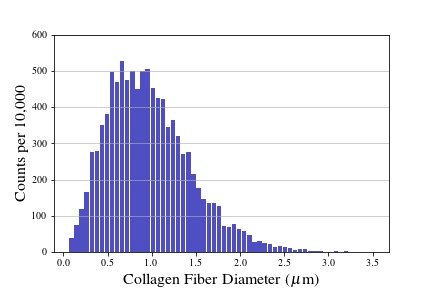
\includegraphics[width=0.45\textwidth]{figures/collagenFiberDiaHistogram.jpg}
    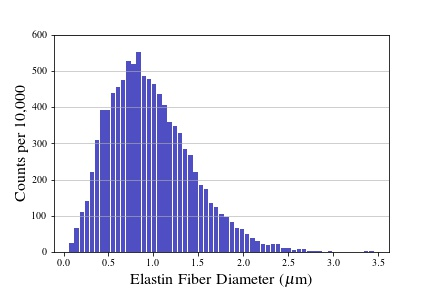
\includegraphics[width=0.45\textwidth]{figures/elastinFiberDiaHistogram.jpg}
    \caption{Typical histograms for collagen and elastin chord diameters pertaining to the statistics reported in Table~\ref{tab:alveolarProp}.  Their tails weigh heavy at the larger diameters, because their distributions are normal in the square root of their diameters.  These histograms are identical, for all practical purposes.}
    \label{fig:septalChordStats}
\end{figure}

The collagen and elastin fibers that make up a septal chord have the same length, they experience the same strain, and they exist at the same temperature; therefore, we employ Eqn.~(\ref{Helmholtz1D}) as the governing constitutive equation to describe their mechanical behavior
\begin{displaymath}
\left\{ \begin{matrix} 
\mathrm{d} \eta \\ \mathrm{d} s
\end{matrix} \right\} = \begin{bmatrix}
C / \theta - E \alpha^2 / \rho & E \alpha / \rho \\
-E  \alpha & E
\end{bmatrix} \left\{ \begin{matrix}
\mathrm{d} \theta \\ \mathrm{d} e
\end{matrix} \right\} 
\end{displaymath}
wherein $\eta$ is the entropy density (erg/gr.K) and $s$ is the chordal stress (barye = $\text{dyne/cm}^2$) in an engineering sense (force per unit reference area) with material constants: $C$ is a specific heat at constant pressure (erg/gr.K), $\alpha$ is a linear coefficient of thermal expansion (1/K), $E$ is an elastic modulus ($\text{dyne/cm}^2$ = $\text{erg/cm}^3$), and $\rho$ is its mass density ($\text{gr/cm}^3$).  Because $\mathrm{d} \theta = 0$ across a wave front \cite{AmesStaff53}, this general system reduces to
\begin{displaymath} 
\mathrm{d} s = E \, \mathrm{d}e
\quad \text{and} \quad
\rho \, \mathrm{d} \eta = E \alpha \, \mathrm{d}e
\end{displaymath} 
wherein the first equation establishes a change in stress carried by a chord, while the second equation establishes a change in entropy per unit volume of chord. 

\subsubsection{Chordal Forces and Entropies}

The constitutive equations that govern alveolar chords, suitable for studying shock waves in lungs, are described by the following equations
\begin{subequations}
    \label{septalChordCEs}
    \begin{align}
    F^f & = s^c A^c + s^e A^e &
    \mathrm{d} s^c & = E^c ( e, s^c ) \, \mathrm{d}e & 
    \mathrm{d} s^e & = E^e ( e, s^e ) \, \mathrm{d}e \\
    S^f & = S^c + S^e & 
    S^c & = S_0^c + \alpha^c s^c V^c & 
    S^e & = S_0^e + \alpha^e s^e V^e
    \end{align}
\end{subequations}  
wherein $F^f$ (dyne) is the fiber force carried by a septal chord, with $s^c$ and $s^e$ being the engineering stresses carried by its collagen and elastin fibers that when multiplied by their reference cross-sectional areas $A^c$ and $A^e$ gives rise to the forces they carry.  Variable $S^f$ (erg/K) denotes the fiber entropy of a septal chord, with $S^c$ and $S^e$ being the entropies of its two parts.  For initial conditions, let $s^c_0 = s^c |_{L = L_0} = 0$ and $s^e_0 = s^e |_{L = L_0} = 0$, and let $S_0^c = \rho^c V^c \eta^c$ and $S_0^e = \rho^e V^e \eta^e$, wherein $\rho^c$ and $\rho^e$ are the mass densities, which are constant because their volumes $V^c$ and $V^e$ are taken to be conserved, while $\eta^c$ and $\eta^e$ are the entropy densities at rest.  It remains to establish the two tangent moduli $E^c (e, s^c)$ and $E^e (e, s^e)$ for collagen and elastin.  These tangent moduli are considered to be implicit functions of state in our modeling of alveolar chords below, see e.g., Ref.~\cite{FreedRajagopal16}.

Collagen is a fiber comprised of numerous, long, slender, wavy filaments whose waviness, known as crimp, straightens under sufficient deformation \cite{Kastelicetal'78,FreedDoehring05}.  Elastin is a linked fiber network, much like an elastomer, whose filaments between crosslinks rotate to align with an axis of loading under sufficient deformation \cite{AaronGosline81,Urry89}.  Consequently, collagen and elastin both recruit constituent filaments with increasing deformation into an overall, load-bearing, fiber response.  The internal energies of collagen and elastin may therefore be thought of as being comprised of a configurational energy and a strain energy.  As such, both collagen and elastin are modeled as Freed-Rajagopal biologic fibers, which are described in terms of two such energies.  Their model is derived from the theory of implicit elasticity in \ref{appImplicitElasticity}.  According to their model, tangent compliances for collagen and elastin are described by
\begin{subequations}
    \label{septalChordModuli}
    \begin{align}
	\frac{1}{E^c (\theta, e, s^c)} & = \frac{e_t^c - e_1^c}{E_1^c e_t^c + 2s^c} + \frac{1}{E_2^c} &
	e_1^c & = e - \alpha^c (\theta - \theta_0) - \frac{s^c}{E_2^c} \\
    \frac{1}{E^e (\theta , e , s^e )} & = \frac{e_t^e - e_1^e}{E_1^e e_t^e + 2s^e} + \frac{1}{E_2^e} &
    e_1^e & = e - \alpha^e (\theta - \theta_0) - \frac{s^e}{E_2^e} 
    \end{align}
\end{subequations}
where material constants $E_1^c$ and $E_2^c$ are two asymptotic moduli for collagen bounding the response, i.e., $E_1^c \leq E^c \leq E^c_2$, while $E_1^e$ and $E_2^e$ are two asymptotic moduli for elastin bounding its response, viz., $E^e_1 \leq E^e \leq E^e_2$, all of which here have units of stress (barye = dyne/$\text{cm}^2$), with $e_t^c$ and $e_t^e$ being their respective transition strains, cf.\ \ref{appImplicitElasticity}. 

The material properties needed to model septal chords are listed in Tables~\ref{tab:alveolarProp} \& \ref{tableCollagenElastin}.  From Eqn.~(\ref{thermodynamicConstraints}), these moduli are bound from above by $E^c_{\max} = 4.9 \times 10^9$~barye ($\text{dyne/cm}^2$) and $E^e_{\max} = 1.7 \times 10^9$~barye.  We therefore observe that $E^c_2$ and $E^e_2$ are about 100 times smaller than $E^c_{\max}$ and $E^e_{\max}$.  We recall that $\theta = \theta_0$ in our application, so the $e^c_1$ and $e^e_1$ strains defined in the second column above simplify somewhat.  

\begin{table}
    \centering
    \begin{tabular}{|l|l|l|}
        \hline
        \multicolumn{3}{|c|}{Collagen$\vphantom{|^{|^|}}$} \\ \hline
        $\rho^c$ \hfill [$\textrm{gr/cm}^{3^{\phantom{|}}}$] & $1.34$ & 
        Fels \cite{Fels64} \\
        $\eta^c$ \hfill [erg/gr.K] & $3.7 \times 10^4$ &  \\
        $C^c$ \hfill [erg/gr.K] & $1.7 \times 10^7$ & 
        Kanagy \cite{Kanagy55} \\
        $\alpha^c$ \hfill [1/C] & $1.8 \times 10^{-4}$ & 
        Weir \cite{Weir48}  \\
        $e^c_t$ & $0.09$ & estimated from TLC $\approx$ 30\% \\
        $E_1^c$ \hfill [barye] & $5.0 \times 10^5$ &  \\
        $E_2^c$ \hfill [barye] & $3.0 \times 10^7$ &  \\ \hline
        \multicolumn{3}{|c|}{Elastin$\vphantom{|^{|^|}}$} \\ \hline 
        Parameter & Value & Reference \\ \hline
        $\rho^e$ \hfill [$\textrm{gr/cm}^{3^{\phantom{|}}}$] & $1.31$ & 
        Lillie \& Gosline \cite{LillieGosline02a} \\
        $\eta^e$ \hfill [erg/gr.K] & $3.4 \times 10^4$ & 
        Shadwick \& Gosline \cite{ShadwickGosline85} \\
        $C^e$ \hfill [$\textrm{erg/gr.K}$] & $4.2 \times 10^7$  & 
        Kakivaya \& Hoeve \cite{KakivayaHoeve75} \\
        $\alpha^e$ \hfill [1/C] & $3.2\times 10^{-4}$ & 
        Lillie \& Gosline \cite{LillieGosline02a} \\ 
        $e^e_t$ & 0.4 & Shadwick \& Gosline \cite{ShadwickGosline85} \\
        $E^e_1$ \hfill [barye] & $2.3 \times 10^6$ & Urry \cite[Fig.~18]{Urry89} \\ 
        $E^e_2$ \hfill [barye] & $1.0 \times 10^7$ & 
        Lillie \& Gosline \cite[Fig.~5]{LillieGosline07} \\ \hline
    \end{tabular}
    \caption{Physical properties for hydrated collagen and elastin fibers.  Collagen denatures at around $60^\circ$C \cite{HoermannSchlebusch71}, i.e., above this temperature collagen will shrink rapidly---an effect not modeled here.}
    \label{tableCollagenElastin}
\end{table}

The actual force and entropy carried by an individual septal chord in our alveolar model will be one third of their calculated values from Eqn.~(\ref{septalChordCEs}), because each chord is typically shared between three neighboring alveoli.

\subsection{Conjugate Pairs $\Longleftrightarrow$ Tensor Components for a Membrane}
\label{secConjugatePairs}

The above planar strains and their rates are defined accordingly \cite{Freedetal17}
\begin{subequations}
    \label{conjugateStrains}
    \begin{align}
    \xi & \defeq \ln \sqrt{\frac{a}{a_0} \frac{b}{b_0}} = 
    \ln \sqrt{\frac{A}{A_0}} &
    \varepsilon & \defeq \ln \sqrt{\frac{b_0}{a_0} \frac{a}{b}} = 
    \ln \sqrt{\frac{\Gamma}{\Gamma_0}} &
    \gamma & \defeq g - g_0 \label{thermoStrains3} \\
    \mathrm{d} \xi & \hspace{2.5pt} = \frac{1}{2} 
    \left( \frac{\mathrm{d} a}{a} + \frac{\mathrm{d} b}{b} \right) = 
    \frac{1}{2} \frac{\mathrm{d} A}{A} &
    \mathrm{d} \varepsilon & \hspace{2.5pt} = \frac{1}{2} 
    \left( \frac{\mathrm{d}a}{a} - \frac{\mathrm{d}b}{b} \right) = 
    \frac{1}{2} \frac{\mathrm{d} \Gamma}{\Gamma} & 
    \mathrm{d} \gamma & \hspace{2.5pt} = \mathrm{d} g
    \label{thermoStrainRates3} 
    \end{align}
\end{subequations}
where $a, b, g$ are the physical attributes illustrated in Fig.~\ref{figKinematics}, with $a_0 , b_0 , g_0$ being their reference values, which are selected so that $\xi_0 = \varepsilon_0 = \gamma_0 = 0$, as established in Part~\ref{partKinematics} via a Gram-Schmidt factorization of the deformation gradient.  These strains are two-state fields, independent of path---a tacit requirement of thermo\-dynamics \cite{Caratheodory09}.  We point out that $\xi = \ln \sqrt{A / A_0}$ where $A = ab$ denotes area, and $\varepsilon = \ln \sqrt{\Gamma / \Gamma_0}$ where $\Gamma = a/b$ denotes the stretch of squeeze, i.e., the stretch of a pure shear deformation is in the sense of Becker \cite{Becker93} and Treloar \cite{Treloar75}. Thermo\-dynamic strains $\xi , \varepsilon , \gamma$ and their differential rates $\mathrm{d} \xi , \mathrm{d} \varepsilon , \mathrm{d} \gamma$ are exported by class \texttt{pentagon} according to Freed \& Zamani \cite{FreedZamani18}, cf.\ \ref{appPentagons}.

The conjugate stresses to the above planar strains are determined to be
\begin{subequations}
    \label{conjugateStresses}
    \begin{align}
    s^{\pi} & \defeq \frac{\pi}{w} = \mathcal{S}_{11} + \mathcal{S}_{22} & 
    s^{\sigma} & \defeq \frac{\sigma}{w} = \mathcal{S}_{11} - \mathcal{S}_{22} & 
    s^{\tau} & \defeq \frac{\tau}{w} = \Gamma \mathcal{S}_{21}
    \label{thermoStresses3} \\
    \intertext{which follow from Eqns.~(\ref{convectedWorkRate} \& \ref{thermoStrainRates3}).  Here $w$ denotes a reference width or thickness of a membrane, i.e., $s^{\pi}$, $s^{\sigma}$ and $s^{\tau}$ are engineering stresses.  Consequently, components $\mathcal{S}_{ij}$ now have units of stress ($\text{dyne/cm}^2$) instead of surface tension (dyne/cm).  Conversely, the physical components of stress $\mathcal{S}_{ij}$ are established through}
    \mathcal{S}_{11} & = \tfrac{1}{2} ( s^{\pi} + s^{\sigma} ) &
    \mathcal{S}_{22} & = \tfrac{1}{2}( s^{\pi} - s^{\sigma} ) &
    \mathcal{S}_{12} & = \mathcal{S}_{21} = s^{\tau}  / \, \Gamma
    \label{stresses3}
    \end{align}
\end{subequations} 
when described in terms of their thermo\-dynamic attributes $s^{\pi}$, $s^{\sigma}$ and $s^{\tau}$, plus the squeeze stretch $\Gamma$ that must appear in $s^{\tau}$ so that $\mathrm{d} \gamma$ associates with an exact differential.  The coupling appearing in the definition for shear stress, viz., $\Gamma \mathcal{S}_{21}$, is the reason why a coupling exists between squeeze and shear in constitutive equation~(\ref{HelmholtzMembraneODEs}).

The stress $\boldsymbol{\mathcal{S}}$ occurring in a septal plane, when evaluated in a pentagonal co-ordinate frame $( \vec{\mathbfit{e}}_{\hspace{0.5pt}1} , \vec{\mathbfit{e}}_{\hspace{0.5pt}2} , \vec{\mathbfit{e}}_{\hspace{0.5pt}3} )$, has non-zero components in the plane, i.e., in the upper-left $2 \times 2$ sub-matrix, with the alveolar pressure $P$ supplying $\mathcal{S}_{33} = -P$.  These components map into a Kirchhoff stress $\mathbf{s}$ expressed in the dodecahedral frame of reference $( \vec{\boldsymbol{\imath}} , \vec{\boldsymbol{\jmath}} , \vec{\mathbfit{k}} )$ via a component transformation of $s_{ij} = P_{ik} Q_{k\ell} \mathcal{R}_{\ell m} \mathcal{S}_{mn} \mathcal{R}_{on} Q_{po} P_{jp}$.   Because $s_{12} = s_{21}$, and because $\mathbf{P}$, $\mathbf{Q}$ and $\boldsymbol{\mathcal{R}}$ are each orthogonal tensors, it necessarily follows that $\mathcal{S}_{12} = \mathcal{S}_{21}$.  Matrix $\mathbf{P}$ is a rotation of the pentagonal frame of reference about that of the dodecahedron's axes, matrix $\mathbf{Q}$ is a rotation for re-indexing pentagonal co-ordinates, and matrix $\boldsymbol{\mathcal{R}}$ is a Gram-Schmidt rotation.

\subsubsection{Modeling an Alveolar Membrane Subjected to a Shock Wave}
  
From a mechanics perspective, we know a great deal more about alveolar chords than we know about alveolar septa.  More judgment will therefore be required in our construction and parameterization of a material model for alveolar membranes.  

A typical alveolar septum is 4-5 $\mu$m in width \cite{Sukietal11}.  They are comprised of an outside layer of epithelial cells that encase capillaries made of endothelial cells along with a basement membrane that is composed of unorganized collagen and elastin filaments, plus proteoglycans and other extracellular proteins.  This basement membrane, roughly at mid-plane in an alveolar septum, has a width of about $0.5 \, \mu$m \cite{RoanWaters11}.  Inertial forces generated by these membranes are to be based upon a membrane thickness of $\sim\!\!5$~$\mu$m with an approximate density of water, while the structural forces that they carry are to be based upon a basement membrane thickness of $\sim\!\! 0.5$~$\mu$m.  

It is not known how much of the mechanical load is actually carried by the cells in an alveolar septum vs.\ the extracellular basement membrane they encase, but it is generally thought that this basement membrane carries the majority of the load \cite{Sukietal11}.  Therefore, by diminishing the moduli that are appropriate for describing a basement membrane with thickness $\sim\!\! 0.5$~$\mu$m by a factor of 10, we get estimates for effective septal moduli that are applicable when modeling a whole septal membrane with thickness $\sim\!\! 5$~$\mu$m.  We use the model parameters obtained for a visceral pleura membrane \cite{Freedetal17} and the above conjecture to model alveolar septa.

From Eqns.~(\ref{HelmholtzMembraneODEsB} \& \ref{conjugateStresses}), alveolar septa are determined to have a constitutive response that, in the presence of shock waves, are governed by
\begin{subequations}
    \begin{align}
\left\{ \begin{matrix}
\mathrm{d} s^{\pi} \\ \mathrm{d} s^{\sigma} \\ \mathrm{d} s^{\tau}
\end{matrix} \right\} & = \begin{bmatrix}
4 M & 0 & 0 \\
0 & 2 N & 2 s^{\tau} \\
0 & 2 s^{\tau} & G
\end{bmatrix} \left\{ \begin{matrix}
\mathrm{d} \xi \\ \mathrm{d} \varepsilon \\ \mathrm{d} \gamma
\end{matrix} \right\} \\
\intertext{that when integrated produce a rotated Kirchhoff stress located at a Gauss point belonging to a pentagon of interest with components}
\begin{bmatrix} 
\mathcal{S}_{11} & \mathcal{S}_{12} & \mathcal{S}_{13} \\
\mathcal{S}_{21} & \mathcal{S}_{22} & \mathcal{S}_{23} \\
\mathcal{S}_{31} & \mathcal{S}_{32} & \mathcal{S}_{33}
\end{bmatrix} & = \begin{bmatrix}
\tfrac{1}{2} ( s^{\pi} + s^{\sigma} ) & b \hspace{0.5pt} s^{\tau} / a & 0 \\
b \hspace{0.5pt} s^{\tau} / a & \tfrac{1}{2} ( s^{\pi} - s^{\sigma} ) & 0 \\
0 & 0 & -P
\end{bmatrix} \label{septalStresses} \\
\intertext{along with a septal (membrane) entropy of}
S^m & = S^m_0 + 2 \alpha s^{\pi} V^m
\end{align}
\end{subequations}
where $S^m$ (erg/K) describes the entropy of a membrane with $S_0^m = \rho^m V^m \eta^m$ denoting its entropy at rest, wherein $\rho^m$ is its mass density, which is constant because its volume $V^m$ is taken to be conserved, and $\eta^m$ is the entropy density at rest, while $\alpha$ is the coefficient of linear thermal expansion, which is twice that of the areal expansion coefficient.  Material constant $M(\xi, s^{\pi})$ is the dilation modulus, $N(\varepsilon, s^{\sigma})$ is the squeeze modulus, and $G(\gamma, s^{\tau})$ is the shear modulus.  All moduli now have units of stress.

Collagen and elastin appear as thin filaments randomly oriented and somewhat uniformly dispersed throughout a basement membrane, unlike the strongly aligned fibers that appear in septal chords.  Consequently, for our purposes, we model this collective ensemble of tissue and structure types as a homo\-geneous isotropic membrane modeled after the Freed-Rajagopal biologic fiber \cite{FreedRajagopal16} that we have extended to membranes in \ref{appImplicitElasticity}, specifically
\begin{subequations}
    \label{septalCompliances}
    \begin{align}
    \frac{1}{M} & = \frac{\xi_t - \xi_1}{M_1 \xi_t + s^{\pi} / 2} + \frac{1}{M_2} &
    \xi_1 & = \xi - \alpha ( \theta - \theta_0 ) - \frac{s^{\pi}}{4M_2}
    \label{septalDilationCompliance} \\
    \frac{1}{N} & = 2 \left( \frac{ \varepsilon_t - | \varepsilon_1 |}{N_1 \varepsilon_t + 2 \gamma s^{\tau}} + \frac{1}{N_2} \right) & 
    \varepsilon_1 & = \varepsilon - \frac{s^{\sigma} - 2 \gamma s^{\tau}}{N_2}
    \label{septalSqueezeCompliance} \\
    \frac{1}{G} & = \Gamma \left( \frac{\gamma_t - 2\varepsilon \gamma - | \gamma_1 |}{G_1 \gamma_t + 2 \varepsilon s^{\tau}} + \frac{1-2\varepsilon}{G_2} \right) & 
    \gamma_1 & = \gamma - \frac{(1 - 2\varepsilon) s^{\tau}}{G_2}
    \label{septalShearCompliance}
    \end{align}
\end{subequations}
where the compliant tangent moduli of $M_1, N_1$ and $G_1$ and the stiff, terminal, tangent moduli of $M_2 , N_2$ and $G_2$ bound their responses in that $M_1 \leq M \leq M_2$, $N_1 \leq N \leq N_2$ and $G_1 \leq G \leq G_2$, with gradual transitions between their asymptotic bounds being centered around strains of $\xi_t , \varepsilon_t$ and $\gamma_t$.

Finite element technology is used to interpolate these stresses to forces at the vertices of a pentagon, cf.\ Part~\ref{partVariational}.  The stress components that actually get interpolated to the element nodes follow from a mapping of $\mathbf{Q} \boldsymbol{\mathcal{RSR}}^{\mathsf{T}} \mathbf{Q}^{\mathsf{T}}$, where $\boldsymbol{\mathcal{R}}$ is the orthogonal rotation coming from the \textbf{QR} decomposition of a deformation gradient, and where $\mathbf{Q}$ is the matrix that re-indexes the co-ordinate indices.  The actual forces and entropy interpolated to these nodes are halved, because each septal plane belongs to two neighboring alveoli. 

\subsection{Modeling an Alveolar Volume Subjected to a Shock Wave}
\label{sec:IdealGasLaw}

Alveoli are connected to bronchial trees via alveolar ducts.  Under normal conditions, air moves in and out of the alveoli via these ducts.  However, when subjected to a stress wave passing over an alveolus, there is no time for the transport of air to take place.  Hence, we can consider the air (and heat) within an alveolus to become `trapped', and the pressure to be uniform therein.  The governing process is therefore adiabatic.  It is under this condition that we model the volumetric response of alveolar sacs.

If one considers the saturated air\slash fluid within an alveolus to be an ideal gas, then \cite{Davison08}
\begin{equation}
P V = n \! R \theta
\quad \text{or} \quad
\frac{P V}{\theta} = \frac{P_0 V_0}{\theta_0} = n \! R = \mathrm{constant}
\label{idealGas}
\end{equation}
where, in our case, $P_0$ is taken to be atmospheric pressure at sea level (1~bar or $10^5$~Pa or $10^6$~barye), with $V_0$ being that alveolar volume whereat alveolar pressure and plural pressure are both atmospheric, while $\theta_0 = 37^{\circ}$C = 310~K is assigned as body temperature.  Parameter $n$ is the molar content of gas within an alveolus, with $R$  being the universal gas constant.  

The material constants associated with an ideal gas contained within an adiabatic enclosure are
\begin{equation}
\alpha \defeq \frac{1}{V} \left. \frac{\partial V}{\partial \theta} \right|_P = 
\frac{1}{\theta_0} \, \frac{P_0 V_0}{P V}
\quad \text{and} \quad
K \defeq -\frac{1}{V} \left. \frac{\partial P}{\partial V} \right|_{\theta} = 
P_0 \, \frac{V_0 \hspace{0.5pt} \theta}{\theta_0 V}
\label{idealGasConstants}
\end{equation}
with the other two material constants pertaining to moist air at body temperature\footnote{
    The physical properties listed for air were taken from the website \texttt{www.peacesoftware.de} hosted by Berndt Wischnewski.
}
being its mass density $\rho$ of $1.125 \times 10^{-3} \; \text{gr/cm}^3$ and its specific heat $C$ at constant pressure of $1.007 \times 10^7$~erg/gr.K, constrained by the fact that $K < K_{\max} = \rho C / \alpha^2 \theta \approx \rho C \theta$.

An alveolar sac is modeled as an adiabatic pressure vessel filled with an ideal gas whose Helmholtz formulation (\ref{Helmholtz3D}) is described by
\begin{equation}
\left\{ \begin{matrix}
\rho \, \mathrm{d} \eta \\ -3 \, \mathrm{d} P
\end{matrix} \right\} = \begin{bmatrix}
\rho C / \theta - K \alpha^2 & 3 K \alpha \\ 
-3K\alpha & 9K
\end{bmatrix} \left\{ \begin{matrix}
\mathrm{d} \theta \\ \mathrm{d} \Xi
\end{matrix} \right\}
\label{alveolarGas}
\end{equation}
that, again, because $\theta = \theta_0$ across a wave front \cite{AmesStaff53}, simplifies the governing system of differential equations (\ref{alveolarGas}) to
\begin{displaymath}
    \mathrm{d}P = -3K \, \mathrm{d} \Xi 
    \quad \text{and} \quad
    \rho \, \mathrm{d} \eta = 3 K \alpha \, \mathrm{d} \Xi
\end{displaymath}
where we recall that $\mathrm{d}\Xi = \tfrac{1}{3} V^{-1} \, \mathrm{d} V$.  Like before, we do not want the entropy per unit mass or per unit volume; rather, we prefer to know what the entropy of its structural constituent is, in this case, the gas within an alveolar sac.  To find this, we multiply the right-hand expression through by volume $V_0$, after which we integrate both differential equations to get
\begin{equation}
    \frac{P}{P_0} = \frac{V_0}{V}
    \quad \therefore \quad
    \alpha = \frac{1}{\theta_0}
    \quad \implies \quad
    S^a = S^a_0 + \frac{V_0 ( P_0 - P )}{\theta_0}
    \label{alveolarSacCE}
\end{equation}
where $S^a$ is the desired entropy of the air within an alveolar sac with $S^a_0 = \rho^a V^a_0 \eta^a$ given that $\rho^a \eta^a$ is the entropy per unit volume of humid air at body temperature and atmospheric pressure, viz., $\rho^a \eta^a = 7.770 \times 10^4 \: \text{erg/cm}^3\text{.K}$.  The above results are in agreement with the ideal gas law, as they should be, because $\alpha$ and $K$ in Eqn.~(\ref{idealGasConstants}) were both derived from this law.

Pressure $P$ is mapped to nodal forces at the vertices of a dodecahedron via Eqn.~(\ref{septalStresses}) in our alveolar model.  This requires finite element technology, which is discussed in Part~\ref{partVariational}.

\section{Code Verification and Constitutive Parameterization}


%\setcounter{equation}{0}
%\setcounter{figure}{0}
%\setcounter{section}{0}
%\setcounter{table}{0}
\part{Numerical Integrators}
\label{partNumericalMethods}

This analysis tool, which models the geometry of alveoli as a dodecahedron, requires numerical methods to integrate the constitutive equations (systems of first-order ODEs), the governing equations of motion (systems of second-order ODEs), and that integrate the length, area or volume of the finite elements (handled using Gaussian quadrature).  The numerical methods used in this work are discussed below.

\section{ODE Solvers}

The various constitutive equations that describe our alveolar model present themselves as ordinary differential equations that need to be integrated.  To this end, we employ the PECE (Predict, Evaluate, Correct, re-Evaluate) algorithms of Freed \cite{Freed17a} which are suitable for solving stiff systems of first- and second-order, ordinary, differential equations.  These methods are based upon Gear's well-known second-order backward difference formula (BDF2, which is Eqn.~\ref{1stOrderCorrector} below).

Time $t$ is considered to be the independent variable, discretized over an interval in time $[t_0, t_N]$ for which $N$ solutions are to be extracted at nodes $n=1, 2, \ldots, N$ spaced at uniform intervals in time with a common step size of $h = (t_N - t_0)/N$ separating them, where time $t_0$ associates with the initial conditions.  This is the \textit{global step size\/} at which solutions are to be gathered.  A dynamically controlled \textit{local step size}, whose size is adjusted on the fly to manage truncation error, is implemented into the code according to a scheme put forward in Ref.~\cite{Soderlind02}.  Solver interfaces are listed in \ref{appSolvers}.

\subsection{PECE Solver for First-Order ODEs}
\label{sec:1stOrderPECE}

Let $\mathbf{x}$ be a vector of dependent variables obeying a differential equation of evolution $\mathrm{d} \mathbf{x}(t) / \mathrm{d} t = \dot{\mathbf{x}} = \mathbf{f} (t, \mathbf{x})$ subject to an initial condition $\mathbf{x}_0 = \mathbf{x}(t_0)$ where $t$ is the independent variable, typically time, but not in our case.

The two-step method put forward here incrementally solves such an ODE, returning solutions associated with the next moment in time $t_{n+1}$, i.e., it acquires $\mathbf{x}_{n+1}$, given knowledge of the  previous $\mathbf{x}_{n-1}$ and current $\mathbf{x}_n$ solutions plus their rates $\dot{\mathbf{x}}_{n-1}$ and $\dot{\mathbf{x}}_n$ with the corrector also depending upon $\dot{\mathbf{x}}_{n+1}$, i.e., the corrector is an implicit method.

\subsubsection{Start-Up Algorithm}

Multi-step methods are not self starting; consequently, Heun's method (a forward-Euler predictor with a trapezoidal corrector) is used here to start our integrator; specifically,
\begin{subequations}
    \label{startUp1stOrderODEs}
    \begin{align}
    \mbox{} & \text{Predict} & 
    \mathbf{x}_1^p & = \mathbf{x}_0 + h \dot{\mathbf{x}}_0 + \mathcal{O} (h^2)
    \label{startUp1stOrderPredictor} \\
    \mbox{} & \text{Evaluate} & 
    \dot{\mathbf{x}}^p_1 & = \mathbf{f} (t_1 , \mathbf{x}_1^p) 
    \label{startUp1stEvaluate} \\
    \mbox{} & \text{Correct} &
    \mathbf{x}_1 & = \mathbf{x}_0 + \tfrac{1}{2} h 
    \bigl( \dot{\mathbf{x}}_1^p + \dot{\mathbf{x}}_0 \bigr) + \mathcal{O} (h^3)
    \label{startUp1stOrderCorrector} \\
    \mbox{} & \text{Re-Evaluate} & 
    \dot{\mathbf{x}}_1 & = \mathbf{f} (t_1 , \mathbf{x}_1) 
    \label{startUp1stReEvaluate}
    \end{align}
\end{subequations}
wherein $\dot{\mathbf{x}}_0 = \mathbf{f}(t_0, \mathbf{x}_0)$ and $t_1 = t_0 + h$.  The correct\slash re-evaluate steps can be iterated over until a convergence criterion is satisfied, if need be.

\subsubsection{Two-Step ODE Solver}

The two-step method of Freed \cite{Freed17a} for solving $1^{\text{st}}$ order ODEs is
\begin{subequations}
    \label{1stOrderODEs}
    \begin{align}
    \mbox{} & \text{Predict} & 
    \mathbf{x}_{n+1}^p & = \tfrac{1}{3} 
    \bigl( 4 \mathbf{x}_n - \mathbf{x}_{n-1} \bigr) + 
    \tfrac{2}{3} h \bigl( 2 \dot{\mathbf{x}}_n - \dot{\mathbf{x}}_{n-1} 
    \bigr) + \mathcal{O} (h^3)
    \label{1stOrderPredictor} \\
    \mbox{} & \text{Evaluate} & 
    \dot{\mathbf{x}}^p_{n+1} & = \mathbf{f} (t_{n+1} , \mathbf{x}_{n+1}^p) 
    \label{1stOrderEvaluate} \\
    \mbox{} & \text{Correct} &
    \mathbf{x}_{n+1} & = \tfrac{1}{3} 
    \bigl( 4 \mathbf{x}_n - \mathbf{x}_{n-1} \bigr) + 
    \tfrac{2}{3} h \dot{\mathbf{x}}^{p}_{n+1} + \mathcal{O} (h^3)
    \label{1stOrderCorrector} \\
    \mbox{} & \text{Re-Evaluate} & 
    \dot{\mathbf{x}}_{n+1} & = \mathbf{f} (t_{n+1} , \mathbf{x}_{n+1}) 
    \label{1stOrderReEvaluate}
    \end{align}
\end{subequations} 
where $t_{n+1} = t_n + h$.  This corrector is the well-known BDF2 formula of Gear to which Freed provided a predictor.  The correct\slash re-evaluate steps can be iterated over until a convergence criterion is satisfied, if need be.  Implementation of this integrator is found in \ref{app1stOrderODEs}.  

For both the predictor and corrector, solution $\mathbf{x}$ has a weight of 1, while its rate $\dot{\mathbf{x}}$ has a weight of $\tfrac{2}{3} h$; hence, this predictor\slash corrector pair is consistent.

\subsection{A Relevant Example}

In our finite element implementation, a hypo-elastic material model \cite{Truesdell55} is introduced to describe the constitutive response of an alveolus in that
\begin{displaymath}
    \dot{\boldsymbol{\sigma}} = \mathbf{M} ( \boldsymbol{\sigma} , \boldsymbol{\epsilon} ) \, \dot{\boldsymbol{\epsilon}} 
    \quad \text{or equivalently \cite{Noll55}} \quad
    \mathrm{d} \boldsymbol{\sigma} = \mathbf{M} ( \boldsymbol{\sigma} , \boldsymbol{\epsilon} ) \, \mathrm{d} \boldsymbol{\epsilon}
\end{displaymath} 
where $\boldsymbol{\epsilon}$ is a vector of thermo\-dynamic strains, $\boldsymbol{\sigma}$ is a vector of thermo\-dynamic stresses, and $\mathbf{M}$ is a square matrix comprised of their tangent moduli, which can depend both upon stress and strain.  In our application, the thermo\-dynamic stress attributes are 
\begin{displaymath}
   \boldsymbol{\sigma}_{1D} = \{ \eta , s \} , \quad
   \boldsymbol{\sigma}_{2D} = \{ \eta , s^{\pi} , s^{\sigma} , s^{\tau} \}^{\mathsf{T}} , \quad
   \boldsymbol{\sigma}_{3D} = \{ \eta , \Pi , \sigma_1 , \sigma_2 , \tau_1 , \tau_2 , \tau_3 \}^{\mathsf{T}}
\end{displaymath}
where $\eta$ is entropy and the rest are stresses, whose thermo\-dynamic conjugates are the strain attributes
\begin{displaymath}
\boldsymbol{\epsilon}_{1D} = \{ \theta , e \} , \quad
\boldsymbol{\epsilon}_{2D} = \{ \theta , \xi , \varepsilon , \gamma \}^{\mathsf{T}} , \quad
\boldsymbol{\epsilon}_{3D} = \{ \theta , \Xi , \varepsilon_1 , \varepsilon_2 , \gamma_1 , \gamma_2 , \gamma_3 \}^{\mathsf{T}}
\end{displaymath}
where $\theta$ is temperature and the rest are strains.  In the 2- and 3-D cases, these stress-strain attributes arise from Gram-Schmidt decompositions of the deformation gradient (cf.\ \S\ref{secQR2D}, \S\ref{secConjugatePairs} and \S\ref{secFE_CE}).  Constructing tangent moduli $\mathbf{M} ( \boldsymbol{\sigma} , \boldsymbol{\epsilon} )$ is the topic of Part~\ref{partConstitutive}.  In the above problem, the thermo\-dynamic strains $\boldsymbol{\epsilon}$ and their differential rates $\mathrm{d} \boldsymbol{\epsilon}$ are known, it is their stresses $\boldsymbol{\sigma}$ that must be integrated.  Both $\boldsymbol{\sigma}$ and $\mathrm{d} \boldsymbol{\sigma} = \mathbf{M} \, \mathrm{d} \boldsymbol{\epsilon}$ arise in the construction of our stiffness matrices, cf.\ \S\ref{secStiffnessMatrices}.

Equation (\ref{startUp1stOrderODEs}) is used to take the first step of integration; specifcally, 
\begin{subequations}
    \notag
    \begin{align}
    \mbox{} & \text{Predict} & 
    \boldsymbol{\sigma}_1^p & = \boldsymbol{\sigma}_0 + h \, \mathrm{d} \boldsymbol{\sigma}_0 \\
    \mbox{} & \text{Evaluate} & 
    \mathrm{d} \boldsymbol{\sigma}^p_1 & = \mathbf{M} ( \boldsymbol{\sigma}_1^p ,
    \boldsymbol{\epsilon} ) \, \mathrm{d} \boldsymbol{\epsilon}_1 \\
    \mbox{} & \text{Correct} &
    \boldsymbol{\sigma}_1 & = \boldsymbol{\sigma}_0 + \tfrac{1}{2} h 
    \bigl( \mathrm{d} \boldsymbol{\sigma}_1^p + 
    \mathrm{d} \boldsymbol{\sigma}_0 \bigr) \\
    \mbox{} & \text{Re-Evaluate} & 
    \mathrm{d} \boldsymbol{\sigma}_1 & = \mathbf{M} ( \boldsymbol{\sigma}_1 , 
    \boldsymbol{\epsilon}_1) \, \mathrm{d} \boldsymbol{\epsilon}_1
    \end{align}
\end{subequations}
where $\mathrm{d} \boldsymbol{\sigma}_0 = \mathbf{M} ( \boldsymbol{\sigma}_0 , \boldsymbol{\epsilon}_0) \, \mathrm{d} \boldsymbol{\epsilon}_0$, with the remaining steps of integration following according to Eqn.~(\ref{1stOrderODEs}), specifically
\begin{subequations}
    \notag
    \begin{align}
    \mbox{} & \text{Predict} & 
    \boldsymbol{\sigma}_{n+1}^p & = \tfrac{1}{3} 
    \bigl( 4 \boldsymbol{\sigma}_n - \boldsymbol{\sigma}_{n-1} \bigr) + 
    \tfrac{2}{3} h \bigl( 2 \, \mathrm{d} \boldsymbol{\sigma}_n - 
    \mathrm{d} \boldsymbol{\sigma}_{n-1} \bigr) \\
    \mbox{} & \text{Evaluate} & 
    \mathrm{d} \boldsymbol{\sigma}^p_{n+1} & = \mathbf{M} ( \boldsymbol{\sigma}_{n+1}^p , \boldsymbol{\epsilon}_{n+1} ) \, 
    \mathrm{d} \boldsymbol{\epsilon}_{n+1} \\
    \mbox{} & \text{Correct} &
    \boldsymbol{\sigma}_{n+1} & = \tfrac{1}{3} 
    \bigl( 4 \boldsymbol{\sigma}_n - \boldsymbol{\sigma}_{n-1} \bigr) + 
    \tfrac{2}{3} h \, \mathrm{d} \boldsymbol{\sigma}^{p}_{n+1}  \\
    \mbox{} & \text{Re-Evaluate} & 
    \mathrm{d} \boldsymbol{\sigma}_{n+1} & = \mathbf{M} ( 
    \boldsymbol{\sigma}_{n+1} , \boldsymbol{\epsilon}_{n+1} )  \,
    \mathrm{d} \boldsymbol{\epsilon}_{n+1}
    \end{align}
\end{subequations} 
where the differential strain rates $\mathrm{d} \boldsymbol{\epsilon}$ are computed via finite differences according to \S\ref{secFE_CE}.


\subsection{PECE Solver for Second-Order ODEs}
\label{sec:2ndOrderPECE}

Let $\mathbf{x}$ be a vector of dependent variables obeying a differential equation of evolution $\mathrm{d}^2 \mathbf{x}(t) / \mathrm{d} t^2 = \ddot{\mathbf{x}} = \mathbf{f} (t, \mathbf{x}, \dot{\mathbf{x}})$ subject to initial conditions $\mathbf{x}_0 = \mathbf{x}(t_0)$ and $\dot{\mathbf{x}}_0 = \dot{\mathbf{x}}(t_0)$.  One may think of $\mathbf{x}$ as being displacements and their rates $\mathbf{v} = \dot{\mathbf{x}}$ as being velocities with $\mathbf{a} = \dot{\mathbf{v}} = \ddot{\mathbf{x}}$ representing accelerations. 

The two-step method put forward here incrementally solves such an ODE, returning solutions associated with the next moment in time $t_{n+1}$, i.e., it acquires $\mathbf{x}_{n+1}$ \& $\dot{\mathbf{x}}_{n+1}$ given knowledge of the previous $\mathbf{x}_{n-1}$ \& $\dot{\mathbf{x}}_{n-1}$ and current $\mathbf{x}_n$ \& $\dot{\mathbf{x}}_n$ solutions plus their accelerations $\ddot{\mathbf{x}}_{n-1}$ and $\ddot{\mathbf{x}}_n$ with the corrector also depending upon $\ddot{\mathbf{x}}_{n+1}$, i.e., the corrector is an implicit method.

\subsubsection{Start-Up Algorithm}

Multi-step methods are not self starting, so a one-step method is needed to take the first step of integration, specifically
\begin{subequations}
    \label{pairedStartUp}
    \begin{align}
    \mbox{} & \text{Predict} & 
    \mathbf{x}_1^p & = \mathbf{x}_0 + h \dot{\mathbf{x}}_0 +
    \tfrac{1}{2} h^2 \ddot{\mathbf{x}}_0 + \mathcal{O} (h^3) 
    \label{startupDisplacementPredictor} \\
    \mbox{} & &
    \dot{\mathbf{x}}^p_1 & = \dot{\mathbf{x}}_0 + h \ddot{\mathbf{x}}_0 + 
    \mathcal{O} (h^2) 
    \label{startUpVelocityPredictor} \\
    \mbox{} & \text{Evaluate} &
    \ddot{\mathbf{x}}^p_1 & = \mathbf{f} (t_1, \mathbf{x}^p_1, \dot{\mathbf{x}}^p_1)
    \label{startUpEvaluate} \\
    \mbox{} & \text{Correct} &
    \mathbf{x}_1 & = \mathbf{x}_0 + \tfrac{1}{2} h 
    \bigl( \dot{\mathbf{x}}^p_1 + \dot{\mathbf{x}}_0 \bigr) -
    \tfrac{1}{12} h^2 \bigl( \ddot{\mathbf{x}}^p_1 - 
    \ddot{\mathbf{x}}_0 \bigr) + \mathcal{O} (h^4) 
    \label{startupDisplacementCorrector} \\
    \mbox{} & &
    \dot{\mathbf{x}}_1 & = \dot{\mathbf{x}}_0 + \tfrac{1}{2} h 
    \bigl( \ddot{\mathbf{x}}_1^p + \ddot{\mathbf{x}}_0 \bigr) + 
    \mathcal{O} (h^3)
    \label{startUpVelocityCorrector} \\
    \mbox{} & \text{Re-Evaluate} &
    \ddot{\mathbf{x}}_1 & = \mathbf{f} (t_1, \mathbf{x}_1, \dot{\mathbf{x}}_1) 
    \label{startUpReEvaluate}
    \end{align}
\end{subequations}
wherein $\ddot{\mathbf{x}}_0 = \mathbf{f}(t_0, \mathbf{x}_0, \dot{\mathbf{x}}_0)$ and $t_1 = t_0 + h$.  The correct\slash re-evaluate steps can be iterated over until a convergence criterion is satisfied, if need be.

\subsubsection{Two-Step ODE Solver}

The two-step method of Freed \cite{Freed17a} for solving $2^{\text{nd}}$ order ODEs is
\begin{subequations}
    \label{pairedMethods}
    \begin{align}
    \mbox{} & \text{Predict} &
    \mathbf{x}_{n+1}^p & = \tfrac{1}{3} \bigl(
    4 \mathbf{x}_n - \mathbf{x}_{n-1} \bigr) + 
    \tfrac{1}{6} h \bigl( 3 \dot{\mathbf{x}}_n + 
    \dot{\mathbf{x}}_{n-1} \bigr) \notag \\ 
    \mbox{} & & & \hspace{3.175cm} + 
    \tfrac{1}{36} h^2 \bigl( 31 \ddot{\mathbf{x}}_n - 
    \ddot{\mathbf{x}}_{n-1} \bigr) + \mathcal{O} (h^4) 
    \label{displacementPredictor} \\
    \mbox{} & &
    \dot{\mathbf{x}}_{n+1}^p & = \tfrac{1}{3} 
    \bigl( 4 \dot{\mathbf{x}}_n - \dot{\mathbf{x}}_{n-1} \bigr) + 
    \tfrac{2}{3} h \bigl( 2\ddot{\mathbf{x}}_n - \ddot{\mathbf{x}}_{n-1} 
    \bigr) + \mathcal{O} (h^3)
    \label{velocityPredictor} \\
    \mbox{} & \text{Evaluate} &
    \ddot{\mathbf{x}}^p_{n+1} & = \mathbf{f} (t_{n+1}, \mathbf{x}^p_{n+1}, \dot{\mathbf{x}}^p_{n+1}) 
    \label{2ndEvaluate} \\
    \mbox{} & \text{Correct} & 
    \mathbf{x}_{n+1} & = \tfrac{1}{3} \bigl(
    4  \mathbf{x}_n - \mathbf{x}_{n-1} \bigr) +
    \tfrac{1}{24} h \bigl( \dot{\mathbf{x}}^p_{n+1} +
    14 \dot{\mathbf{x}}_n + \dot{\mathbf{x}}_{n-1} \bigr) 
    \notag \\
    \mbox{} & & & \hspace{3.175cm} +
    \tfrac{1}{72} h^2 \bigl( 10 \ddot{\mathbf{x}}^p_{n+1} + 
    51 \ddot{\mathbf{x}}_n - \ddot{\mathbf{x}}_{n-1} \bigr) + 
    \mathcal{O} (h^4)
    \label{displacementCorrector} \\ 
    \mbox{} & &
    \dot{\mathbf{x}}_{n+1} & = \tfrac{1}{3} 
    \bigl( 4 \dot{\mathbf{x}}_n - \dot{\mathbf{x}}_{n-1} \bigr) + 
    \tfrac{2}{3} h \ddot{\mathbf{x}}^p_{n+1} + \mathcal{O} (h^3)
    \label{velocityCorrector} \\
    \mbox{} & \text{Re-Evaluate} & 
    \ddot{\mathbf{x}}_{n+1} & = \mathbf{f} (t_{n+1}, \mathbf{x}_{n+1}, \dot{\mathbf{x}}_{n+1})
    \label{2ndReEvaluate}
    \end{align}
\end{subequations}
where $t_{n+1} = t_n + h$.  An implementation of this integrator is described in \ref{app2ndOrderODEs}.  

The above PECE solver for velocity $\dot{\mathbf{x}}$ is the same method presented in Eq.~(\ref{1stOrderODEs}), so this predictor\slash corrector pair is consistent.  Likewise, in both the predictor and corrector for displacement $\mathbf{x}$, contributions from the solution $\mathbf{x}$ have a weight of 1, contributions from the velocities $\dot{\mathbf{x}}$ have a weight of $\tfrac{2}{3} h$, and contributions from the accelerations $\ddot{\mathbf{x}}$ have a weight of $\tfrac{5}{6} h^2$; hence, this predictor\slash corrector pair is consistent, too.

\subsection{A Relevant Example}
\label{sec:solve2ndOrderODE}

The finite element problem that we consider here requires solutions for
\begin{displaymath}
    \mathbf{M} \ddot{\mathbf{u}} + \mathbf{K}\mathbf{u} = \mathbf{f}(t)
\end{displaymath}
where $\mathbf{u}$ is a generalized displacement vector, $\ddot{\mathbf{u}}$ is its acceleration, $\mathbf{M}$ and $\mathbf{K}$ are mass and stiffness matrices, and $\mathbf{f}(t)$ is a forcing function evaluated at current time $t$.  For this system of ODEs, the first step to be taken follows algorithm (\ref{pairedStartUp}) and is implemented as
\begin{subequations}
    \notag
    \begin{align}
    \mbox{} & \text{Predict} & 
    \mathbf{u}_1^p & = \mathbf{u}_0 + h \dot{\mathbf{u}}_0 +
    \tfrac{1}{2} h^2 \ddot{\mathbf{u}}_0 \\
    \mbox{} & &
    \dot{\mathbf{u}}^p_1 & = \dot{\mathbf{u}}_0 + h \ddot{\mathbf{u}}_0 \\
    \mbox{} & \text{Evaluate} &
    \ddot{\mathbf{u}}^p_1 & = \mathbf{M}^{-1} \bigl( \mathbf{f}(t_{1} ) - 
    \mathbf{K} \mathbf{u}_1^p \bigr) \\
    \mbox{} & \text{Correct} &
    \mathbf{u}_1 & = \mathbf{u}_0 + \tfrac{1}{2} h 
    \bigl( \dot{\mathbf{u}}^p_1 + \dot{\mathbf{u}}_0 \bigr) -
    \tfrac{1}{12} h^2 \bigl( \ddot{\mathbf{u}}^p_1 - \ddot{\mathbf{u}}_0 \bigr) \\
    \mbox{} & &
    \dot{\mathbf{u}}_1 & = \dot{\mathbf{u}}_0 + \tfrac{1}{2} h 
    \bigl( \ddot{\mathbf{u}}_1^p + \ddot{\mathbf{u}}_0 \bigr) \\
    \mbox{} & \text{Re-Evaluate} &
    \ddot{\mathbf{u}}_1 & = \mathbf{M}^{-1} \bigl( \mathbf{f}(t_1 ) - 
    \mathbf{K} \mathbf{u}_1 \bigr)
    \end{align}
\end{subequations}
where the CE steps of the PECE sequence can be iterated on to a user-specified tolerance, which increases the methods stability as the corrector is implicit.  Continued solution steps are then governed by algorithm (\ref{pairedMethods}), which takes on the form of
\begin{subequations}
    \notag
    \begin{align}
    \mbox{} & \text{Predict} &
    \mathbf{u}_{n+1}^p & = \tfrac{1}{3} \bigl(
    4 \mathbf{u}_n - \mathbf{u}_{n-1} \bigr) + 
    \tfrac{1}{6} h \bigl( 3 \dot{\mathbf{u}}_n + 
    \dot{\mathbf{u}}_{n-1} \bigr) + 
    \tfrac{1}{36} h^2 \bigl( 31 \ddot{\mathbf{u}}_n - 
    \ddot{\mathbf{u}}_{n-1} \bigr) \\
    \mbox{} & &
    \dot{\mathbf{u}}_{n+1}^p & = \tfrac{1}{3} 
    \bigl( 4 \dot{\mathbf{u}}_n - \dot{\mathbf{u}}_{n-1} \bigr) + 
    \tfrac{2}{3} h \bigl( 2 \ddot{\mathbf{u}}_n - \ddot{\mathbf{u}}_{n-1} \bigr) \\
    \mbox{} & \text{Evaluate} &
    \ddot{\mathbf{u}}^p_{n+1} & = \mathbf{M}^{-1} \bigl( \mathbf{f}(t_{n+1} ) - 
    \mathbf{K} \mathbf{u}_{n+1}^p \bigr) \\
    \mbox{} & \text{Correct} & 
    \mathbf{u}_{n+1} & = \tfrac{1}{3} \bigl(
    4  \mathbf{u}_n - \mathbf{u}_{n-1} \bigr) +
    \tfrac{1}{24} h \bigl( \dot{\mathbf{u}}^p_{n+1} +
    14 \dot{\mathbf{u}}_n + \dot{\mathbf{u}}_{n-1} \bigr)  \\
    \mbox{} & & & \hspace{3.175cm} +
    \tfrac{1}{72} h^2 \bigl( 10 \ddot{\mathbf{u}}^p_{n+1} + 
    51 \ddot{\mathbf{u}}_n - \ddot{\mathbf{u}}_{n-1} \bigr) \\ 
    \mbox{} & &
    \dot{\mathbf{u}}_{n+1} & = \tfrac{1}{3} 
    \bigl( 4 \dot{\mathbf{u}}_n - \dot{\mathbf{u}}_{n-1} \bigr) + 
    \tfrac{2}{3} h \ddot{\mathbf{u}}^p_{n+1}  \\
    \mbox{} & \text{Re-Evaluate} & 
    \ddot{\mathbf{u}}_{n+1} & = \mathbf{M}^{-1} \bigl( \mathbf{f}(t_{n+1} ) - 
    \mathbf{K} \mathbf{u}_{n+1} \bigr) 
    \end{align}
\end{subequations}
where, again, the CE steps of the PECE sequence can be iterated on to a user-specified tolerance.  In this problem, velocities $\dot{\mathbf{u}}$ are not needed for the evaluation steps, but they are required by the prediction and correction steps of integration.

We observe that the mass matrix must not be ill conditioned in order for this algorithm to work as intended.  Since the mass matrix does not change with time, it only needs to be evaluated and inverted once.  This is an advantage over using the popular Newmark \cite{Newmark59} integrator where matrix inversion is required at every step along a solution path.

\section{Quadrature Rules for Spatial Integration}
\label{secGauss}

Three Gauss quadrature rules are given here for alveolar chords, alveolar septa and for tetrahedra that fill an alveolar sac.  These formul\ae\ integrate polynomials of $1^{\text{st}}$, $3^{\text{rd}}$ and $5^{\text{th}}$ degrees, exactly, for the chord and pentagon, and of $1^{\text{st}}$, $2^{\text{nd}}$ and $3^{\text{rd}}$ degrees, exactly, for a tetrahedron.  In all cases, integrating $1^{\text{st}}$ order polynomials takes place at their centroids.

\subsection{Gauss Integration of Alveolar Chords}

The quadrature rules that integrate a 1D chord in its natural co-ordinate system, which spans $-1 \leq \xi \leq 1$, are presented in Table~\ref{tabQuadrature1D}.  These formul\ae\ are well known and can be found in most finite element textbooks.

\begin{table}
    \centering
    \begin{tabular}{|c|rr|}
        \hline
        node & \centering $\xi$ co-ordinate \phantom{1}  & 
        weight \phantom{123} \\ \hline
        & \multicolumn{2}{|c|}{Exact for Polynomials of Degree $1^{\phantom{|^|}}$} \\ 
        \hline
        1 & 0.000000000000 & 2.000000000000 \\ 
        \hline
        & \multicolumn{2}{|c|}{Exact for Polynomials of Degree $3^{\phantom{|^|}}$} \\ \hline
        1 & -0.577350269189 & 1.000000000000\\
        2 & 0.577350269189 & 1.000000000000\\ 
        \hline
        & \multicolumn{2}{|c|}{Exact for Polynomials of Degree $5^{\phantom{|^|}}$} \\ \hline
        1 & -0.774596669241 & 0.555555555556 \\
        2 & 0.000000000000 & 0.888888888889\\
        3 & 0.774596669241 & 0.555555555556\\ 
        \hline
    \end{tabular}
    \caption{Generalized, Gaussian, quadrature weights and nodes for integrating over an alveolar chord in its natural co-ordinate system.  These weights sum to 2, the span of its natural co-ordinate.}
    \label{tabQuadrature1D}
\end{table}

\subsection{Gauss Integration of Alveolar Septa}

Three, Gauss, quadrature rules for a regular pentagon described in its natural coordinate system, i.e., oriented according to Fig.~\ref{figRegPentagon}, are presented in Table~\ref{tabQuadrature}.  These quadratures exactly integrate polynomials of order 1, 3 and 5, respectively.  They were supplied to the authors by Prof.\ N.\ Sukumar from the University of California at Davis, which he derived for us at our request using a methodology that he published in \cite{Mousavietal10}.  In that document, the authors derived formul\ae\ for determining the nodes and weights for a class of generalized, Gaussian, quadrature rules, which they then applied to pentagons, hexagons, heptagons and octagons, of which they only published their nodes and weights of quadrature for the hexagon, as it tiles two space.  The node for the $1^{\mathrm{st}}$ order method is located at the centroid.  Nodes for the $3^{\mathrm{rd}}$ and $5^{\mathrm{th}}$ order methods of Table~\ref{tabQuadrature} are displayed in Fig.~\ref{figQuadrature}.

\begin{table}
    \centering
    \begin{tabular}{|c|rrr|}
        \hline
        node & \centering $\xi$ coordinate \phantom{123}  & 
        $\eta$ coordinate \phantom{123} & weight \phantom{12345} \\ \hline
        & \multicolumn{3}{|c|}{Exact for Polynomials of Degree $1^{\phantom{|^|}}$} \\ \hline
        1 & 0.0000000000000000 & 0.0000000000000000 &
        2.3776412907378837\vphantom{$|^{|^|}$} \\ 
        \hline
        & \multicolumn{3}{|c|}{Exact for Polynomials of Degree $3^{\phantom{|^|}}$} \\ \hline
        1 & -0.0349156305831802 &  0.6469731019095136 &
        0.5449124407446143\vphantom{$|^{|^|}$} \\
        2 & -0.5951653065516678 & -0.0321196846022659 & 0.6439082046243272 \\
        3 &  0.0349156305831798 & -0.6469731019095134 & 0.5449124407446146 \\
        4 &  0.5951653065516677 &  0.0321196846022661 & 0.6439082046243275 \\ 
        \hline
        & \multicolumn{3}{|c|}{Exact for Polynomials of Degree $5^{\phantom{|^|}}$} \\ \hline
        1 & -0.0000000000000000 & -0.0000000000000002 &
        0.6257871064166934\vphantom{$|^{|^|}$} \\
        2 & -0.1351253857178451 &  0.7099621260052327 & 0.3016384608809768 \\
        3 & -0.6970858746672087 &  0.1907259121533272 & 0.3169910433902452 \\ 
        4 & -0.4651171392611024 & -0.5531465782166917 & 0.3155445150066620 \\
        5 &  0.2842948078559476 & -0.6644407817506509 & 0.2958801959111726 \\
        6 &  0.7117958231685716 & -0.1251071394727008 & 0.2575426306970870 \\
        7 &  0.5337947578638855 &  0.4872045224587945 & 0.2642573384350463 \\
        \hline
    \end{tabular}
    \caption{Generalized, Gaussian, quadrature weights and nodes (a.k.a., cubature rules) for integrating over a regular pentagon in its natural coordinate system.  These weights sum to the area of a pentagon inscribing an unit circle, the formula of which is given in Eqn.~(\ref{regPentagonArea}).}
    \label{tabQuadrature}
\end{table}

The Gaussian quadrature rules of Mousavi, Xiao \& Sukumar \cite{Mousavietal10} presented in Table~\ref{tabQuadrature} are compatible with the shape functions of Wachspress \cite{Wachspress75,Wachspress16} and Dasgupta \cite{Dasgupta03} presented in \S\ref{secShapeFns}.

\begin{figure}
    \centering
    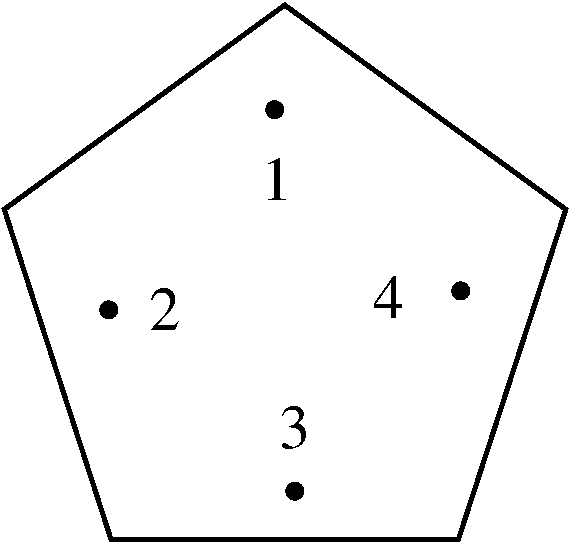
\includegraphics[width=4cm]{figures/pentagon_degree3.pdf}
    \hspace{1cm}
    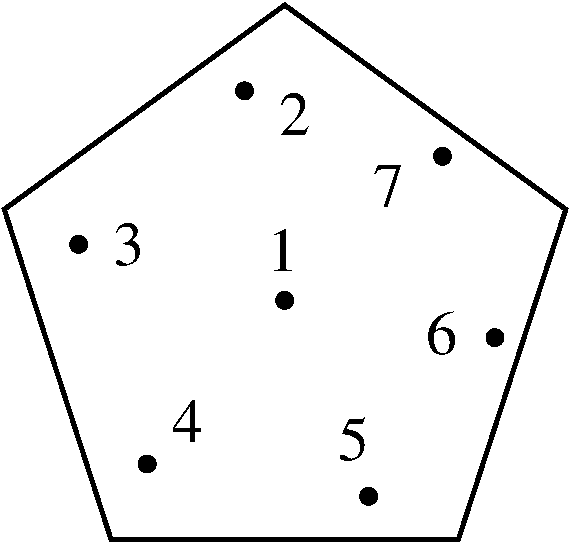
\includegraphics[width=4cm]{figures/pentagon_degree5.pdf}
    \caption{Locations of generalized, Gaussian, quadrature nodes for the $3^{\mathrm{rd}}$ (left) and $5^{\mathrm{th}}$ (right) degree integration methods presented in Table~\ref{tabQuadrature}.  Vertex 1 is located at the top of the pentagon, cf.\ Fig.~\ref{figRegPentagon}, while the coordinate origin is located at its centroid (node 1 in the right figure).}
    \label{figQuadrature}
\end{figure}

\subsection{Gauss Integration of Alveolar Sacs}

The quadrature rules that integrate a 2D tetrahedron in its natural co-ordinate system, where the apex is at the origin, and along its three axes: $0 \leq \xi \leq 1$, $0 \leq \eta \leq 1$ and $0 \leq \zeta \leq 1$.  These formul\ae\ integrate polynomials of $1^{\text{st}}$, $2^{\text{nd}}$ and $3^{\text{rd}}$ degrees, exactly, and can be found in most finite element textbooks.  

\begin{table}
    \centering
    \begin{tabular}{|c|rrrr|}
        \hline
        node & \centering $\xi$ co-ordinate & $\eta$ co-ordinate & 
        $\zeta$ co-ordinate & weight \\ \hline        
        & \multicolumn{4}{|c|}{Exact for Polynomials of Degree $1^{\phantom{|^|}}$} \\ 
        \hline
        1 & 1/4 & 1/4 & 1/4 & 1/6 \\ 
        \hline
        & \multicolumn{4}{|c|}{Exact for Polynomials of Degree $2^{\phantom{|^|}}$} \\ \hline
        1 & (5 - $\sqrt{5}$)/20 & (5 - $\sqrt{5}$)/20 & (5 - $\sqrt{5}$)/20 & 1/24\\
        2 & (5 - $\sqrt{5}$)/20 & (5 - $\sqrt{5}$)/20 & (5 + 3 $\sqrt{5}$)/20 & 1/24\\
        3 & (5 - $\sqrt{5}$)/20 & (5 + 3 $\sqrt{5}$)/20 & (5 - $\sqrt{5}$)/20 & 1/24\\ 
        4 & (5 + 3 $\sqrt{5}$)/20 & (5 - $\sqrt{5}$)/20 & (5 - $\sqrt{5}$)/20 & 1/24\\ 
        \hline
        & \multicolumn{4}{|c|}{Exact for Polynomials of Degree $3^{\phantom{|^|}}$} \\ \hline
        1 & 1/4 & 1/4 & 1/4 & -2/15 \\
        2 & 1/2 & 1/6 & 1/6 & 3/40\\
        3 & 1/6 & 1/2 & 1/6 & 3/40\\ 
        4 & 1/6 & 1/6 & 1/2 & 3/40 \\
        5 & 1/6 & 1/6 & 1/6 & 3/40 \\
        \hline
    \end{tabular}
    \caption{Generalized, Gaussian, quadrature weights and nodes for integrating over a tetrahedron in its natural co-ordinate system.  These weights sum to \textfrac{1}{6}, which is the volume of a tetrahedron measured in its natural co-ordinate system.}
    \label{tabQuadraturetetra}
\end{table} 


%\setcounter{equation}{0}
%\setcounter{figure}{0}
%\setcounter{section}{0}
%\setcounter{table}{0}
\setcounter{section}{0}
\part{Variational Formulation}
\label{partVariational}

The problem we have set up to solve takes on the general form of 
\begin{equation}
	\mathbf{M} \ddot{\mathbf{x}} + \mathbf{K} \mathbf{x} = \mathbf{f}(t)
\end{equation}
where $\mathbf{M}$ is a mass matrix, $\mathbf{K}$ is a stiffness matrix, $\mathbf{f}$ is a forcing function, and $\mathbf{x}$ is a displacement vector.  

For our problem of interest, 
\begin{subequations}
\begin{align}
	\mathbf{x} & = \sum_{v=1}^{20} \{ x_v , y_v , z_v \}^{\mathsf{T}} \\
	\intertext{are the co-ordinates of vertex $v$ located in the co-ordinate frame of the dodecahedron $(\boldsymbol{\imath} , \boldsymbol{\jmath} , \vec{\mathbfit{k}} )$ so that vectors $\mathbf{f}$ and $\mathbf{x}$ have length 60 while matrices $\mathbf{M}$ and $\mathbf{K}$ have dimension $60 \times 60$ with}
	\mathbf{M} & = \mathbf{M}_{1D} + \mathbf{M}_{2D} + \mathbf{M}_{3D} \\
	\mathbf{K} & = \mathbf{K}_{1D} + \mathbf{K}_{2D} + \mathbf{K}_{3D} \\
	\mathbf{f} & = \mathbf{f}_{1D} + \mathbf{f}_{2D} + \mathbf{f}_{3D}
\end{align}
\end{subequations}
where subscript `$\mbox{}_{1D}$' applies to the alveolar chords, subscript `$\mbox{}_{2D}$' applies to the alveolar septa, and subscript `$\mbox{}_{3D}$' applies to the alveolar volume.

\section{Mass Matrix}
A consistent mass matrix \cite{Archer65} established in its natural co-ordinate system is defined as
\begin{equation}
	\mathbf{M} = \sum_m \int_{V_m} \rho_m \, \mathbf{N}_m^{\mathsf{T}} \mathbf{N}_m \,
	\mathrm{d} V_m
	\label{consistentMassMatrix}
\end{equation}
wherein $\mathbf{N}_m$ is the shape function matrix used to also construct the stiffness matrix for element $m$.

\subsection{Mass Matrix of Chord}
The determinant of the Jacobian matrix is used for the transformation of integral from the global coordinate system to the natural coordinate system by
\begin{equation}
     |J| = \mathrm{\det} J =  \frac{\partial x }{\partial\xi} = \sum\nolimits_{i=1}^n N_{i,\xi} (\xi) \, x_i
\end{equation}
wherein $N_{i}$ are the shape functions for a two-node alveolar chords in its natural coordinate system which are defined in a matrix form as
\begin{equation}
	\mathbf{N} = \begin{bmatrix}
    \frac{1}{2} \, (1 - \xi) &  \frac{1}{2} \, (1 + \xi)
\end{bmatrix} 
\end{equation}
wherein $\xi$ is abscissae of the Gauss integration rule. 

The consistent mass matrix of the 1-D alveolar chord that is evaluated numerically in its natural coordinate system can be described as
\begin{equation}
    \mathbf{M}_{1C} = \int_{\Gamma} \rho \, \mathbf{N}^{\mathsf{T}} \mathbf{N} \, A \, \mathrm{d} x  = \int_{-1}^{1} \rho \, \mathbf{N}^{\mathsf{T}} \mathbf{N}\, A \, |\mathbf{J}|\,  \mathrm{d} \xi =  \sum_{i=1}^{n}  \rho  \, \mathbf{N}^{\mathsf{T}} \mathbf{N} \, A\, |\mathbf{J}| \, \mathrm{w}_i
\end{equation}
 with $\mathrm{w}_i$ being the  weighting coefficients of the Gauss integration rule, and $A$ being the cross section area of alveolar chord. Table~\ref{tabQuadrature1D} demonstrates the values of $\xi$ and $\mathrm{w}_i$ for $n = 1, 2$, and $3$ Gauss integration points.
\begin{table}
    \centering
    \begin{tabular}{|c|rr|}
        \hline
        node & \centering $\xi$ coordinate \phantom{12}  & 
        weight \phantom{12} \\ \hline
        & \multicolumn{2}{|c|}{Exact for Polynomials of Degree $1^{\phantom{|^|}}$} \\ 
        \hline
        1 & 0.0000000000000 & 2.0000000000000 \\ 
        \hline
        & \multicolumn{2}{|c|}{Exact for Polynomials of Degree $3^{\phantom{|^|}}$} \\ \hline
        1 & -0.577350269189 & 1.000000000000\\
        2 & 0.577350269189 & 1.000000000000\\ 
        \hline
        & \multicolumn{2}{|c|}{Exact for Polynomials of Degree $5^{\phantom{|^|}}$} \\ \hline
        1 & -0.774596669241 & 0.555555555556 \\
        2 & 0.000000000000 & 0.888888888889\\
        3 & 0.774596669241 & 0.555555555556\\ 
        \hline
    \end{tabular}
    \caption{Generalized, Gaussian, quadrature, weights and nodes for integrating over a alveolar chord in its natural coordinate system.}
    \label{tabQuadrature1D}
\end{table}

The row-sum techniques is considered to construct the lumped mass matrix for 1-D alveolar chord, that is the sum of the elements of each row of the consistent mass matrix is used as the diagonal element \cite{Reddy93}:
\begin{equation}
{M}_{1L_{ii}} = \sum_{j=1}^n \int_{\Gamma} \rho \, N_i \, N_j \, A \, \mathrm{d} x  = \int_{-1}^{1} \rho \, N_i\, A \, |\mathbf{J}|\,  \mathrm{d} \xi =  \sum_{i=1}^n  \rho  \, N_i\, A\, |\mathbf{J}| \, \mathrm{w}_i
\end{equation}
wherein $\sum_{j=1}^n N_j = 1$. 

The lumped-consistent weighted mass matrix $\mathbf{M}_{1LC} $ of the 1-D alveolar chord is defined as 
\begin{equation}
\mathbf{M}_{1LC}  = (1 - \mu) \, \mathbf{M}_{1C} + \mu \, \mathbf{M}_{1L}
\label{LumconsMass1D}
\end{equation}
wherein $\mu$ is a free scalar parameter that is considered to be $\mu = 1/2$ to minimize low frequency dispersion.


For instance, the consistent mass matrix for alveolar chords with $1$ Gauss integration point that is approximated by the weighted sum of function at the center of chord becomes
\begin{equation}
\mathbf{M}_{1C}  = \frac{\rho \, A \, L}{4}\begin{bmatrix}
1 & 1 \\
1 & 1
\end{bmatrix} 
	\label{ConsMassMatrix1D}
\end{equation}
where $L$ is the length of alveolar chord. The row-sum techniques, gives the lumped mass matrix
\begin{equation}
\mathbf{M}_{1L}  = \frac{\rho \, A \, L}{2}\begin{bmatrix}
1 & 0 \\
0 & 1
\end{bmatrix} 
\label{LumMassMatrix1D}
\end{equation}
and the lumped-consistent weighted mass matrix is constructed as follow 
\begin{equation}
\mathbf{M}_{1LC}  = \frac{\rho \, A \, L}{8}\begin{bmatrix}
3 & 1 \\
1 & 3
\end{bmatrix} 
\label{LumconsMassMatrix1D}
\end{equation}


\subsection{Mass Matrix of Pentagon}
For the alveolar septa, the matrix of shape functions $\mathbf{N}$ is arranged as
 \begin{equation}
	\mathbf{N} = 
	\begin{bmatrix}
	N_1 & 0 & N_2 & 0 & N_3 & 0 & N_4 & 0 & N_5 & 0 \\ 0 & N_1 & 0 & N_2 & 0 & N_3 & 0 & N_4 & 0 & N_5 
\end{bmatrix} 
	\label{shape2D}
\end{equation}
in which $\mathrm{N}_i (i = 1, 2, 3, 4, 5)$ are five shape functions corresponding to the five vertices of the pentagon that are defined in Eq.~(\ref{shapeFunctions}).
The consistent mass matrix $\mathbf{M}_{2C}$ can also be obtained by substituting the above shape function matrix into 
\begin{equation}
    \mathbf{M}_{2C} = \int_{V} \rho \, \mathbf{N}^{\mathsf{T}} \mathbf{N} \, \mathrm{d} V = \int_{\pentagon} \int_{\pentagon} \rho \, \mathbf{N}^{\mathsf{T}} \mathbf{N} \,|\mathbf{J}| \, h \, \mathrm{d} \xi \, \mathrm{d} \eta
    \label{massintegral2d}
\end{equation}
wherein $h$ being membrane thickness, and $|\mathbf{J}|$ being the determinant of the Jacobian matrix for pentagon. 
In quadrilateral derivations,  the Jacobian of two-dimensional transformations that connect the ${x, y}$ to ${\xi, \eta}$ coordinate systems is needed. The components of Jacobian matrix are calculated using derivatives of shape functions with respect to the local and the current global coordinates at the $i^{\mathrm{th}}$ vertex via
\begin{equation}
[\mathbf{J}] = 
\begin{bmatrix}
\partial x / \partial\xi & \partial y / \partial\xi \\
\partial x / \partial\eta & \partial y / \partial\eta 
\end{bmatrix}  
= \begin{bmatrix}
\sum\nolimits_{i=1}^5 N_{i,\xi} (\xi,\eta) \, x_i & \sum\nolimits_{i=1}^5 N_{i,\xi} (\xi,\eta) \, y_i \\
\sum\nolimits_{i=1}^5 N_{i,\eta} (\xi,\eta) \, x_i & \sum\nolimits_{i=1}^5 N_{i,\eta} (\xi,\eta) \, y_i
\end{bmatrix}
\label{jacobianpent}
\end{equation}
The numerical integration of Eq.~(\ref{massintegral2d}) result in 
\begin{equation}
    \mathbf{M}_{2C} = \sum_{p=1}^{n} \rho \, \mathbf{N}^{\mathsf{T}} \mathbf{N} \,|\mathbf{J}| \, h \, w_i
\end{equation}
where $n$ stands for number of Gauss points, and $\mathrm{w}_i$ denotes the natural weight of the element.
There are three mass matrix for each pentagon based upon three Gauss, quadrature rules in Table~\ref{tabQuadrature} which are integrating polynomials of order 3 and 5, respectively. 

The row-sum techniques is considered to construct the Lumped mass matrix for pentagon, that makes the diagonal parameters as follow
\begin{equation}
{M}_{2L_{ii}} = \sum_{j=1}^n \int_{V}  \rho \, N_i \, N_j \, A \, \mathrm{d} V  = \int_{\pentagon} \int_{\pentagon} \rho \, N_i\, A \, |\mathbf{J}|\,  \mathrm{d} \xi \, \mathrm{d} \eta =  \sum_{i=1}^n  \rho  \, N_i\, h\, |\mathbf{J}| \, \mathrm{w}_i
\label{LumMass2D}
\end{equation}
wherein $\sum_{j=1}^n N_j = 1$. 

The lumped-consistent weighted mass matrix $\mathbf{M}_{2LC} $ for the 2-D alveolar septa by choosing $\mu = 1/2$ is defined as 
\begin{equation}
\mathbf{M}_{2LC}  = (1 - \mu) \, \mathbf{M}_{2C} + \mu \, \mathbf{M}_{2L} = \frac{1}{2} \, (\mathbf{M}_{2C} + \mathbf{M}_{2L})
\label{LumconsMass2D}
\end{equation}
For instance,the lumped-consistent mass matrix of a pentagon  with $1$ Gauss integration point at the center of pentagon that is constructed by averaging consistent mass matrix and the lumped mass matrix becomes 
\begin{equation}
\mathbf{M}_{2LC}  = \rho \, h
\begin{bmatrix}
0.28532 & 0 & 0.04755 & 0 & 0.04755 & 0 & 0.04755 & 0 \\ 0.04755 & 0 \\
0 & 0.28532 & 0 & 0.04755 & 0 & 0.04755 & 0 & 0.04755\\ 0 & 0.04755
\\
0.04755 & 0 & 0.28532 & 0 & 0.04755 & 0 & 0.04755 & 0 \\ 0.04755 & 0\\
0 & 0.04755 & 0 & 0.28532 & 0 & 0.04755 & 0 & 0.04755\\ 0 & 0.04755 \\
0.04755 & 0 & 0.04755 & 0 & 0.28532 & 0 & 0.04755 & 0 \\ 0.04755 & 0 \\
0 & 0.04755 & 0 & 0.04755 & 0 & 0.28532 & 0 & 0.04755\\ 0 & 0.04755 \\
0.04755 & 0 & 0.04755 & 0 & 0.04755 & 0 & 0.28532 & 0\\ 0.04755 & 0\\
0 & 0.04755 & 0 & 0.04755 & 0 & 0.04755 & 0 & 0.28532\\ 0 & 0.04755\\
0.04755 & 0 & 0.04755 & 0 & 0.04755 & 0 & 0.04755 & 0 \\ 0.28532 & 0 & 0.04755\\
0 & 0.04755 & 0 & 0.04755 & 0 & 0.04755 & 0 & 0.04755\\ 0 & 0.28532\\
\end{bmatrix} 
\label{LumconsMassMatrix2D}
\end{equation}


\subsection{Mass Matrix of Tetrahedron}

The dodecahedron has 60 individual tetrahedral whereas its origin being the common vertex of all tetrahedrons. Hence, the analysis to find the mass matrix of a tetrahedron is used to reach the mass matrix of whole alveolar volume.

The matrix of shape functions $\mathbf{N}$ for a tetrahedon has the form of
\begin{equation}
	\mathbf{N} =  
\begin{bmatrix*}[r]
	N_1 & 0 & 0 & N_2 & 0 & 0 & N_3 & 0 & 0 & N_4 & 0 & 0 \\
	0 & N_1 & 0 & 0 & N_2 & 0 & 0 & N_3 & 0 & 0 & N_4 & 0 \\
	0 & 0 & N_1 & 0 & 0 & N_2 & 0 & 0 & N_3 & 0 & 0 & N_4
\end{bmatrix*} 
	\label{shape3D}
\end{equation}
in which $\mathrm{N}_i (i = 1, 2, 3, 4)$ are four shape functions corresponding to the four vertices of the tetrahedron that are defined as follow
\begin{subequations}
\begin{align}
	N_1 & = 1 - \xi - \eta - \zeta \\
	N_2 & = \xi \\
	N_3 & = \eta \\
	N_4 & = \zeta
\end{align}
\end{subequations}
The numerical integration is used to obtain the mass matrix of tetrahedron via
\begin{equation}
    \mathbf{M}_{3D} = \sum_{p=1}^{n_p} \rho  \mathbf{N}^{\mathsf{T}} \mathbf{N} \,  \,|\mathbf{J}| \, w_p
\end{equation}
wherein $|\mathbf{J}|$ being the determinant of the Jacobian matrix in a tetrahedron that are calculated using derivatives of shape functions with respect to the local coordinates $(\xi, \eta, \zeta)$, and the current global coordinates $(x_i, y_i, z_i)$ at the $i^{\mathrm{th}}$ vertex via
\begin{equation}
\begin{aligned}
\left[\mathbf{J}\right]= &
\begin{bmatrix}
\partial x / \partial\xi & \partial y / \partial\xi & \partial z / \partial\xi\\
\partial x / \partial\eta & \partial y / \partial\eta & \partial z / \partial\eta \\
\partial x / \partial\zeta & \partial y / \partial\zeta & \partial z / \partial\zeta 
\end{bmatrix}\\
  = & \begin{bmatrix}
\sum\nolimits_{i=1}^4 N_{i,\xi} (\xi,\eta,\zeta) \, x_i & \sum\nolimits_{i=1}^4 N_{i,\xi} (\xi,\eta,\zeta) \, y_i &
\sum\nolimits_{i=1}^4 N_{i,\xi} (\xi,\eta,\zeta) \, z_i\\
\sum\nolimits_{i=1}^4 N_{i,\eta} (\xi,\eta,\zeta) \, x_i & \sum\nolimits_{i=1}^4 N_{i,\eta} (\xi,\eta,\zeta) \, y_i &
\sum\nolimits_{i=1}^4 N_{i,\eta} (\xi,\eta,\zeta) \, z_i\\
\sum\nolimits_{i=1}^4 N_{i,\zeta} (\xi,\eta,\zeta) \, x_i & \sum\nolimits_{i=1}^4 N_{i,\zeta} (\xi,\eta,\zeta) \, y_i &
\sum\nolimits_{i=1}^4 N_{i,\zeta} (\xi,\eta,\zeta) \, z_i
\end{bmatrix}
\end{aligned}
\label{jacobiantet}
\end{equation}

There are three mass matrix for each tetrahedron based upon three Gauss, quadrature rules in Table~\ref{tabQuadraturetetra} which are integrating polynomials of order 1, 2 and 3, respectively. 

\begin{table}
    \centering
    \begin{tabular}{|c|rrrr|}
        \hline
        node & \centering $\xi$ coordinate \phantom{1234}  & 
        $\eta$ coordinate \phantom{1234} & 
        $\zeta$ coordinate \phantom{1234} & weight \phantom{12345} \\ \hline        
        & \multicolumn{4}{|c|}{Exact for Polynomials of Degree $1^{\phantom{|^|}}$} \\ 
        \hline
        1 & 1/4 & 1/4 & 1/4 & 1/6 \\ 
        \hline
        & \multicolumn{4}{|c|}{Exact for Polynomials of Degree $2^{\phantom{|^|}}$} \\ \hline
        1 & (5 - $\sqrt{5}$)/20 & (5 - $\sqrt{5}$)/20 & (5 - $\sqrt{5}$)/20 & 1/24\\
        2 & (5 - $\sqrt{5}$)/20 & (5 - $\sqrt{5}$)/20 & (5 + 3 $\sqrt{5}$)/20 & 1/24\\
        3 & (5 - $\sqrt{5}$)/20 & (5 + 3 $\sqrt{5}$)/20 & (5 - $\sqrt{5}$)/20 & 1/24\\ 
        4 & (5 + 3 $\sqrt{5}$)/20 & (5 - $\sqrt{5}$)/20 & (5 - $\sqrt{5}$)/20 & 1/24\\ 
        \hline
        & \multicolumn{4}{|c|}{Exact for Polynomials of Degree $3^{\phantom{|^|}}$} \\ \hline
        1 & 1/4 & 1/4 & 1/4 & -2/15 \\
        2 & 1/6 & 1/6 & 1/6 & 3/40\\
        3 & 1/6 & 1/6 & 1/2 & 3/40\\ 
        4 & 1/6 & 1/2 & 1/6 & 3/40 \\
        5 & 1/2 & 1/6 & 1/6 & 3/40 \\
        \hline
    \end{tabular}
    \caption{Generalized, Gaussian, quadrature, weights and nodes  for integrating over a tetrahedron in its natural coordinate system.}
    \label{tabQuadraturetetra}
\end{table}


The row-sum techniques is considered to construct the lumped mass matrix for pentagon, that makes the diagonal parameters as follow
\begin{equation}
{M}_{3L_{ii}} = \sum_{j=1}^n \int_{V}  \rho \, N_i \, N_j \, A \, \mathrm{d} V = \sum_{i=1}^n  \rho  \, N_i\, |\mathbf{J}| \, \mathrm{w}_i
\label{LumMass3D}
\end{equation}

wherein $\sum_{j=1}^n N_j = 1$. 

The lumped-consistent weighted mass matrix $\mathbf{M}_{3LC} $ for the 3-D alveolar volume by choosing $\mu = 1/2$ becomes 
\begin{equation}
\mathbf{M}_{3LC}  = (1 - \mu) \, \mathbf{M}_{3C} + \mu \, \mathbf{M}_{3L} = \frac{1}{2} \, (\mathbf{M}_{3C} + \mathbf{M}_{3L})
\label{LumconsMass3D}
\end{equation}



%\setcounter{equation}{0}
%\setcounter{figure}{0}
%\setcounter{section}{0}
%\setcounter{table}{0}
\section{Conclusions}
\label{partConclusions}

This report develops a micro\-scopic alveolar model whose homogenized response describes the macro\-scopic behavior of parenchyma in lung.  Such a model can be used in lieu of physical experiments to help develop and parameterize a better continuum lung model for use in finite element analyses.   The need for such a model is to aid Army engineers in their development of improved PPE to better protect Soldiers from BABT and BLI when impacted by ballistic projectiles or blast waves.  

The geometry of an individual alveolus is modeled as an irregular dodecahedron comprising 20 alveolar vertices, 30 1D alveolar chords, and 12 2D pentagonal alveolar septa, all enveloping a 3D alveolar sac.  Implicit elastic constitutive equations are used to model these alveolar chords and septa.  Alveolar chords are modeled as collagen and elastin fibers loaded in parallel.  Damage is accounted for through the rupture of individual alveolar fibers and septa, and the tearing of capillaries that lead to blood and interstitial fluids leaking into its alveolar sac.  Material properties for the individual fibers and septa are assigned through probability distribution functions to account for their biologic variability.

It is shown that geometric strains for the three physical dimensions that arise in this analysis are equivalent during uniform deformations when they are defined as: $\ln (L / L_0)$ for 1D rods, $\ln \sqrt{A / \! A_0}$ for 2D membranes, and $\ln \sqrt[3]{V \! / V_0}$ for 3D volumes.  Adopting Laplace stretch as our fundamental kinematic variable, thermo\-dynamic conjugate pairs are established for these three geometric dimensions.  These thermo\-dynamic strains equate with the above geometric strains under conditions of uniform deformation, plus they allow for the handling of nonuniform deformations, in particular, pure and simple shears.

New to this report are:  \textit{i\/}) Sets of consistent interpolation\slash extrapolation procedures for 1D rods, 2D triangles and pentagons, and 3D tetrahedra, which allow physical fields to be mapped between the nodes and Gauss points of an element in a reproducible manner; \textit{ii\/}) Shape functions and a Gauss integration formula suitable for constructing a pentagonal finite element, which is used to model alveolar septa; \textit{iii\/}) Nonlinear strain-displacement matrices for 2D pentagons and 3D tetrahedra that employ Laplace stretch as their kinematic variable; and \textit{iv\/})  A numerical algorithm that employs both secant and tangent stiffness matrices in its finite element solver.


%\setcounter{part}{6}
%\setcounter{section}{6}
%\renewcommand{\thesection}{\arabic{section}}

\arlbibliography[f]{dodec}%	Provide name of .bib file as argument

% Appendices

\setcounter{equation}{0}
\setcounter{figure}{0}
\setcounter{section}{0}
\setcounter{table}{0}
\appendix{Implicit Elasticity}
\label{appImplicitElasticity}

Both explicit (i.e., Green \cite{Green41}) and implicit (i.e., Rajagopal \cite{Rajagopal03}) elastic material models are put forward in this appendix for one's consideration when choosing a material model to represent biologic fibers and membranes.  We discuss thermo\-elastic fibers first, and then thermo\-elastic membranes.  We have no need to address thermo\-elastic bodies in 3D for our application, beyond what has been presented in \S\ref{sec:IdealGasLaw}.  In this appendix, we employ Gibbs free-energy potential $\mathcal{G}$ instead of the internal energy potential $U$, which we employ in the body of this report.  These potentials relate to one another through a well-known Legendre transformation.  A Gibbs energy approach implies that a change in the intensive variables (thermo\-dynamic forces) will cause a response in the extensive variables (thermo\-dynamic displacements), which is the exact opposite cause-and-effect arising from an internal energy approach.  Causality is correct whenever one uses a Gibbs approach, from a physics perspective.  Nevertheless, applications often find other approaches to be more useful, especially that of Helmholtz.  Here we present both secant and tangent moduli formulations for biologic fibers and membranes, as both are required by our variational formulation.

\subsection{Alveolar Chords as Green (Explicit) Thermoelastic Fibers}

For a 1D fiber with a mass density of $\rho$ per unit length, the thermo\-dynamic conjugate fields are: temperature $\theta$ and entropy $\eta$, plus force $F$ and length $L$, whose initial values in some reference configuration are denoted as $\theta_0$, $\eta_0$, $F_0$ and $L_0$.  In our construction, it is insightful to use $\ln (\theta / \theta_0)$ and $\ln (L/L_0)$ as measures for change in temperature and length, with the former changing how we interpret thermal strain, but not specific heat, while the latter is commonly referred to as mechanical strain, viz., $e \defeq \ln (L/L_0)$.

A Green thermo\-elastic fiber has a Gibbs free-energy potential described by an explicit function of state, viz., $\mathcal{G} (\theta , F)$ where $\mathrm{d} \mathcal{G} = -\eta \, \mathrm{d} \theta - \tfrac{1}{\rho} e \, \mathrm{d}F$ (cf.~Eqn.~\ref{thermoelastic1Dlaw}), out of which one derives the governing thermo\-elastic constitutive equations, viz., for entropy
\begin{subequations}
    \label{thermoelasticFiber}
    \begin{align}
    \eta & = - \partial_{\theta\,} \mathcal{G} (\theta , F) ,
    \label{fiberEntropy} \\
    \intertext{and for strain}
    e & \defeq \ln ( L / L_0 ) = -\rho \, \partial_{F\,} \mathcal{G} (\theta, F) . 
    \label{fiberStrain}
    \end{align}
\end{subequations}
Providing an energy function establishes a material model.

\subsubsection{Hookean Fibers}

Herein we consider a Gibbs free-energy potential suitable for describing a Hookean fiber, i.e.,
\begin{multline}
    \mathcal{G} (\theta , F) = -\eta_0 (\theta - \theta_0) -
    C \left( \theta \ln \left( \frac{\theta}{\theta_0} \right) - (\theta - \theta_0) \right) \\ - 
    \frac{F - F_0}{\rho} \left( \alpha \ln \left( \frac{\theta}{\theta_0} \right) + \frac{F - F_0}{2E}  \right)
    \label{GreenFiberEnergy}
\end{multline}
normalized so that $\mathcal{G}(\theta_0 , F_0) = 0$ with initial conditions of $\eta_0 = -\partial_{\theta\,} \mathcal{G} (\theta_0 , F_0)$ and $e_0 = -\rho \, \partial_F \mathcal{G} (\theta_0 , F_0) = 0$ in our reference state associated with fields $\theta_0$ and $F_0$.   

The model's material properties are: a specific heat $C$, a thermal strain coefficient $\alpha$, and an elastic compliance $1/E$ or modulus $E$.  These properties are interpreted from the perspective of both secant and tangent functions of state in this appendix.

\textit{In~vivo}, biologic fibers operate under cyclic loading conditions where, typically, \mbox{$0 < F_{\min} < F < F_{\max} < F_{\mathrm{ult}}$} that, under normal physiologic conditions, finds force $F$ traversing between $F_{\min}$ and $F_{\max}$ with $F_{\mathrm{ult}}$ designating ultimate rupture strength.  Here we take $F_0$ to associate with $F_{\min}$.  Consequently, strain is assigned to be zero in this reference state of $F_0>0$.  Similarly, physicians will reference against some physiologic state of relevance; however, their reference states usually associate with $F_{\max}$, not $F_{\min}$, e.g., total lung capacity for pulmonary applications, and max systole for cardiac applications.  \textit{Ex~vivo}, one typically selects $F_0 = 0$ for biologic fibers.

\subsubsection{Secant Material Properties}

Upon subtituting the Gibbs free-energy function (\ref{GreenFiberEnergy}) into the constitutive equations (\ref{fiberEntropy} \& \ref{fiberStrain}) governing entropy and strain, respectively, results in the matrix expression
\begin{displaymath}
\left\{ \begin{matrix}
\eta - \eta_0 \\ \ln (L / L_0)
\end{matrix} \right\} = \begin{bmatrix}
C_s & \alpha_s / \rho \theta \\
\alpha_s & 1 / E_s
\end{bmatrix} \left\{ \begin{matrix}
\ln ( \theta / \theta_0 ) \\ F - F_0
\end{matrix} \right\}
\end{displaymath}
which rearranges into a form that is more suitable for our needs, specifically
\begin{subequations}
    \label{HookeanFiberModel}
    \begin{align}
    \left\{ \begin{matrix}
        \eta - \eta_0 \\ F - F_0
    \end{matrix} \right\} & = \begin{bmatrix}
        C_s - \alpha^2_s E_s / \rho \theta & 
        \alpha_s E_s / \rho \theta \\
        -\alpha_s E_s & E_s
    \end{bmatrix} \left\{ \begin{matrix}
        \ln ( \theta / \theta_0 ) \\ \ln (L / L_0)
    \end{matrix} \right\}
    \label{elasticHookeanFiber} \\
    \intertext{with material properties: a specific heat (evaluated at some reference force $F_0$) of}
    C_s & \defeq 
    \left. \frac{\eta - \eta_0}{\ln( \theta / \theta_0 )}
    \right|_{F=F_0} 
    \label{secantSpecificHeat} \\
    \intertext{with $C_s - \alpha^2_s E_s / \rho \theta$ being a heat capacity (evaluated at some reference length $L_0$), plus a thermal strain coefficient (evaluated at some reference force $F_0$) of}
    \alpha_s & \defeq \left. \frac{\ln(L/L_0)}{\ln(\theta/\theta_0)}
    \right|_{F=F_0} ,
    \label{secantThermalExpansion} \\
    \intertext{and an elastic compliance (evaluated at some reference temperature $\theta_0$) of}
    \frac{1}{E_s} & \defeq \left. \frac{\ln(L/L_0)}{F - F_0} \right|_{\theta=\theta_0} .
    \end{align}
\end{subequations}
These are \textit{secant\/} material properties, hence the subscript `$s$', which can be measured through appropriate experiments.  The curves that they trace through state space are then to be approximated via a model.

\textbf{Note}: Thermal elongation is typically modeled as $\alpha (\theta - \theta_0)$, wherein $\alpha$ is referred to as the coefficient for thermal expansion.  Our thermal strain coefficient $\alpha_s$, which is dimensionless, and the coefficient for thermal expansion $\alpha$, which has dimensions of reciprocal temperature, relate via $\alpha_s = \alpha \theta_0 + \mathcal{O}\bigl( ((\theta - \theta_0) / \theta_0)^2 \bigr)$ because $\ln ( \theta / \theta_0 ) = (\theta - \theta_0) / \theta_0 - (\theta - \theta_0)^2 / \theta_0^2 + (\theta - \theta_0)^3 / \theta_0^3 - \cdots$.

\subsubsection{Tangent Material Properties}

Upon differentiating the constitutive equations for entropy and strain found in Eqns.\ (\ref{fiberEntropy} \& \ref{fiberStrain}), respectively, assuming that they are both sufficiently differentiable functions of state, while adopting the expression for Gibbs free energy found in Eqn.~(\ref{GreenFiberEnergy}), results in the following constitutive equation
\begin{displaymath}
\left\{ \begin{matrix}
\mathrm{d} \eta \\ L^{-1} \, \mathrm{d} L 
\end{matrix} \right\} = -\begin{bmatrix}
\partial_{\theta\theta\,} \mathcal{G} & \partial_{\theta F\,} \mathcal{G} \\
\rho \, \partial_{F\theta\,} \mathcal{G} & \rho \, \partial_{FF\,} \mathcal{G}
\end{bmatrix} 
\left\{ \begin{matrix}
\mathrm{d} \theta \\ \mathrm{d} F
\end{matrix} \right\}
= \begin{bmatrix}
C_t & \alpha_t / \rho \theta \\
\alpha_t & 1 / E_t
\end{bmatrix}
\left\{ \begin{matrix}
\theta^{-1} \, \mathrm{d} \theta \\ \mathrm{d} F
\end{matrix} \right\}
\end{displaymath}
where we observe that the intensive and extensive variables now appear in rate or differential form; hence, this formulation is hypo-elastic. \cite{Truesdell55}  This matrix equation can be rearranged into an expression that is more suitable for our needs, viz.,
\begin{subequations}
    \label{fiberConstitutiveTheory}
    \begin{align}
    \left\{ \begin{matrix}
        \mathrm{d} \eta \\ \mathrm{d} F
    \end{matrix} \right\} & = \begin{bmatrix}
        C_t - \alpha^2_t E_t / \rho \theta & 
        \alpha_t E_t / \rho \theta \\
        -\alpha_t E_t & E_t
    \end{bmatrix} \left\{ \begin{matrix}
       \theta^{-1} \, \mathrm{d} \theta \\
       L^{-1} \, \mathrm{d} L
    \end{matrix} \right\} 
    \label{thermoelasticCE1D} \\
    \intertext{whose material properties are: a specific heat (at constant force) of}
    C_t & \defeq
    \left. \frac{\mathrm{d} \eta}{\theta^{-1} \, \mathrm{d} \theta} 
    \right|_{\mathrm{d}F=0} = C_s - \frac{\alpha_s (F - F_0)}{\rho \, \theta} = -\theta \, \partial_{\theta\theta\,} \mathcal{G} (\theta, F) 
    \label{specificHeat} \\
    \intertext{where the tangent response for specific heat $C_t$ relates to the secant response for specific heat $C_s$ via $C_t = C_s - \alpha_s (F - F_0) / \rho \theta$, with $C_t - \alpha_t^2 E_t / \rho \theta$ being a heat capacity (at constant strain), plus a thermal strain coefficient (at constant force) of}
    \alpha_t & \defeq 
    \left. \frac{L^{-1} \, \mathrm{d}L}
    {\theta^{-1} \, \mathrm{d}\theta} \right|_{\mathrm{dF=0}} =
    -\rho\theta \, \partial_{F\theta\,} \mathcal{G} (\theta , F) =
    -\rho\theta \, \partial_{\theta F\,} \mathcal{G} (\theta , F) 
    \label{thermalExpansion} \\
    \intertext{where, typically, $\alpha_t \equiv \alpha_s$, and an elastic compliance (at constant temperature) of}
    \frac{1}{E_t} & \defeq 
    \left. \frac{L^{-1} \, \mathrm{d}L}{\mathrm{d}F}
    \right|_{\mathrm{d}\theta=0} =
    -\rho \, \partial_{FF\,} \mathcal{G} (\theta , F) 
    \label{compliance}
    \end{align}
\end{subequations}
which is distinct from its secant compliance for the biologic fiber model that follows.  These are \textit{tangent\/} material properties, hence the subscript `$t$', whose values can be measured through appropriate experiments.

Matrix equation (\ref{thermoelasticCE1D}) is expressed in terms of Helmholtz causality, but is derived out of Gibbs causality to ensure that Maxwell's condition (present in Eqns.~\ref{thermoelasticCE1D} \& \ref{thermalExpansion}) is satisfied.

It turns out that these tangent material properties correspond directly with components acquired from the Laplacian of one's Gibbs free-energy potential.

\subsection{Alveolar Chords as Rajagopal (Implicit) Thermoelastic Fibers}

In 2003, Rajagopal \cite{Rajagopal03} introduced the idea of an implicit elastic solid.  In 2016, Freed \&\ Rajagopal \cite{FreedRajagopal16} constructed an elastic fiber model that convolves an explicit energy with an implicit energy.  In their approach, they decomposed fiber strain $e \defeq \ln (L / L_0)$ into a sum of two strains, viz., $e = e_1 + e_2$ wherein $e_1 \defeq \ln (L_1 / L_0)$ and $e_2 \defeq \ln (L / L_1)$.  Length $L_0$ is a reference fiber length, viz., its length whereat $F = F_0$.  Length $L_1$ can be thought of as the fiber's length caused solely by a molecular reconfiguration under an applied load of $F$ (e.g., an unraveling of crimp in collagen, a network reorientation in elastin, a reconformation in structural proteins, etc.).  The state associated with length $L_1$ is non-physical in that one cannot unravel molecules without also stretching some of their bonds to a certain extent.  Final length $L$ is the actual fiber length under an applied load $F$ caused by both a reconfiguration and a stretching of its molecular network.  Here we present their ideas in terms of a Gibbs free-energy function, which leads naturally to additive compliances, instead of working with moduli, which do not add.\footnote{%
    Freed \& Rajagopal \cite{FreedRajagopal16} originally used a Helmholtz free-energy function.
}

Let the Gibbs free-energy potential be described by a function of the form\footnote{
    One might be tempted to consider an implicit energy function of the form $\mathcal{G} = \mathcal{G}_1 (\theta ,  e , F ) + \mathcal{G}_2 (\theta , F)$, but this would lead to a non-symmetric susceptibility matrix.  Consequently, it would not satisfy Maxwell's thermo\-dynamic constraint, a.k.a.\ Sylvester's condition for integrability of a Pfaffian form.  Hence, it is an inadmissible functional dependence for a Gibbs potential.
}
\begin{equation}
\mathcal{G} (\theta , e , F) \defeq \mathcal{G}_1 ( e_1 , F ) + \mathcal{G}_2 ( \theta , F )
\quad \text{with} \quad
\mathrm{d} \mathcal{G} = -\eta \, \mathrm{d} \theta - 
\tfrac{1}{\rho} e \, \mathrm{d} F
\label{GibbsFreeEnergy}
\end{equation}
where $\mathcal{G}_1$ is an implicit potential (a configuration energy) and $\mathcal{G}_2$ is an explicit potential (a strain energy).  This energy function leads to the same constitutive equation displayed in Eqn.~(\ref{thermoelasticCE1D}), but whose material properties from Eqns.~(\ref{specificHeat}--\ref{compliance}) are now interpreted according to the following formul\ae
\begin{subequations}
    \label{physicalFields1Dfiber}
    \begin{align}
    C_t & \defeq 
    \left. \frac{\mathrm{d} \eta}{\theta^{-1} \, \mathrm{d} \theta} 
    \right|_{\mathrm{d}F=0} \; =
    -\theta \, \partial_{\theta\theta\,} \mathcal{G} ( \theta , e , F ) = 
    -\theta \, \partial_{\theta\theta\,} \mathcal{G}_2(\theta , F)
    \label{specificHeat1D} \\
    \alpha_t & \defeq
    \left. \frac{L^{-1} \, \mathrm{d}L}
    {\theta^{-1} \, \mathrm{d}\theta} \right|_{\mathrm{dF=0}} =
    -\rho\theta \, \partial_{F\theta\,} \mathcal{G} (\theta , e , F) =
    -\rho\theta \, \partial_{F\theta\,} \mathcal{G}_2(\theta , F)
    \label{thermalExpansion1D} \\
    \frac{1}{E_t} & \defeq 
    \left. \frac{L^{-1} \, \mathrm{d}L}{\mathrm{d}F}
    \right|_{\mathrm{d}\theta=0} = -
    \bigl( \rho \, \partial_{e_1} \mathcal{G}_1 ( e_1 , F ) \bigr)^{-1} 
    \bigl( e + \rho \, \partial_{F\,} \mathcal{G} (\theta , e , F) \bigr) \notag \\ \mbox{} & \hspace{33mm} -
    \rho \, \partial_{FF\,} \mathcal{G}_2(\theta , F)
    \label{compliance1D}
    \end{align}
\end{subequations}
where mass density $\rho$ is a mass per unit length of line.  Elastic compliance $1/E_t$ is now found to be a sum of two compliances, independent of the functional forms that one might select for $\mathcal{G}_1 ( e_1 , F )$ and $\mathcal{G}_2 ( \theta , F )$.  One compliance is explicit in origin, i.e., $e_2 = -\rho \, \partial_{F\,} \mathcal{G}_2$ with rate $\mathrm{d} e_2 = -\rho \, \partial_{F\theta\,} \mathcal{G}_2 \, \mathrm{d} \theta - \rho \, \partial_{FF\,} \mathcal{G}_2 \, \mathrm{d}F$.  It comprises the second row in Eqn.~(\ref{compliance1D}).  The other compliance is implicit in origin, viz., $\mathrm{d} e_1 = - ( \rho \, \partial_{e_1 \,} \mathcal{G}_1 )^{-1} ( e_1 + \rho \, \partial_{F\,} \mathcal{G}_1 ) \mathrm{d}F \equiv - ( \rho \, \partial_{e_1 \,} \mathcal{G}_1 )^{-1} ( e + \rho \, \partial_{F\,} \mathcal{G} ) \mathrm{d}F$.  It comprises the first row in Eqn.~(\ref{compliance1D}). Also, $\partial_{F\theta\,} \mathcal{G} = \partial_{\theta F\,} \mathcal{G}$ because of Maxwell's thermo\-dynamic constraint.

The material properties of Eqn.~(\ref{physicalFields1Dfiber}) apply to matrix equation~(\ref{thermoelasticCE1D}), just as those for a Hookean material do, viz., Eqns.~\ref{specificHeat}--\ref{compliance}).  The specific heat $C_t$ and thermal strain coefficient $\alpha_t$ have the same interpretations for both explicit and implicit fiber theories.  It is with respect to their compliances through which they differ.

\medskip\noindent
\textbf{Derivation}: 
Because Gibbs free energy is a state function, its differential describes a Pfaffian form, and as such, the left-hand side of the thermo\-dynamic expression $\mathrm{d} \mathcal{G} = -\eta \, \mathrm{d} \theta - \tfrac{1}{\rho} e \, \mathrm{d}F$ becomes $\mathrm{d} \mathcal{G} = \partial_{e_1} \mathcal{G}_1 \, \mathrm{d} e_1 + \partial_{F\,} \mathcal{G}_1 \, \mathrm{d}F + \partial_{\theta\,} \mathcal{G}_2 \, \mathrm{d} \theta + \partial_{F\,} \mathcal{G}_2 \, \mathrm{d}F$. Recalling that $e = e_1 + e_2$, the explicit (hyper-elastic like) terms combine to produce constitutive equations
\begin{displaymath}
\eta = -\partial_{\theta\,} \mathcal{G}_2 (\theta , F) 
\quad \text{and} \quad
e_2 = -\rho \, \partial_{F\,} \mathcal{G}_2 (\theta , F)
\end{displaymath} 
while the remaining implicit terms collect to yield a differential constitutive equation of the form
\begin{displaymath}
\rho \, \partial_{e_1} \mathcal{G}_1 ( e_1 , F ) \, \mathrm{d} e_1 = 
-\bigl( e_1 + \rho \, \partial_{F\,} \mathcal{G}_1 ( e_1 , F )
\bigr) \mathrm{d}F .
\end{displaymath}
Differentiating the constitutive equation for entropy with respect to state leads directly to expressions for the specific heat $C_t$ and the thermal expansion coefficient $\alpha_t$ stated in Eqns.~(\ref{specificHeat1D} \& \ref{thermalExpansion1D}).  Recalling that the strains add, i.e., $e = e_1 + e_2$, and therefore so do their rates, viz., $\mathrm{d} e = \mathrm{d} e_1 + \mathrm{d} e_2$, a direct consequence of them being logarithmic in construction, it follows that upon rearranging the implicit constitutive equation to solve for $\mathrm{d} e_1$, while differentiating the explicit constitutive equation for $e_2$, and finally adding these strain increments to get $\mathrm{d} e$, one obtains the elastic compliance function stated in Eqn.~(\ref{compliance1D}).  \hfill $\qed$

\subsubsection{Biologic Fibers with Tangent Material Properties}
\label{secBioFiber}

The fiber model of Freed \&\ Rajagopal \cite{FreedRajagopal16} imposes a limiting constraint $e_{1_{\max}}$ onto the internal strain of reconfiguration $e_1$, viz., $e_1 \leq e_{1_{\max}}$.  Their model, when cast in terms of a Gibbs free-energy function in the form of Eqn.~(\ref{GibbsFreeEnergy}), is described by an implicit energy contribution of\footnote{
    In the paper of Freed \&\ Rajagopal \cite{FreedRajagopal16}, they adopted a Helmholtz free-energy potential of the form $E e_1 - F + \beta e_1 F$ where $\beta$ is a material parameter that relates to a limiting state of strain.  Here we adopt a Gibbs free-energy potential of like form, specifically $e_{1_{\max}} (E e_1 - F) + 2e_1 F$ where $e_{1_{\max}}$ is this limiting state of internal strain $e_1$.  We point out that an exponential response akin to Fung's material models will result whenever the energy of reconfiguration takes on a form of $E e_1 - F$.
}
\begin{subequations}
    \label{RajagopaleanFiber}
    \begin{align}
    \mathcal{G}_1 ( e_1 , F ) & = - \frac{1}{\rho} \Bigl(
    e_{1_{\max}} \bigl( E_1 e_1 - (F - F_0) \bigr) + 
    2 e_1 (F - F_0) \Bigr)
    \label{FreedEnergy} \\
    \intertext{and and explicit energy contribution of}
    \mathcal{G}_2(\theta , F) & = -\eta_0 (\theta - \theta_0) -
    C \left( \theta \ln \left( \frac{\theta}{\theta_0} \right) - 
    (\theta - \theta_0) \right) \notag \\ 
    \mbox{} & \qquad - \frac{F - F_0}{\rho} 
    \left( \alpha \ln \left( \frac{\theta}{\theta_0} \right) + \frac{F - F_0}{2E_2} \right)
    \label{HookeanEnergy} \\
    \intertext{that, collectively, depend upon tempreature $\theta$, force $F$, and an internal strain $e_1$, whose free energy is normalized so that $\mathcal{G}_1(e_{1,0}, F_0) = 0$ and $\mathcal{G}_2(\theta_0, F_0)=0$ with initial conditions $e_{1,0}=0$, $e_{2,0} = -\rho \, \partial_{F\,} \mathcal{G}_2 ( \theta_0 , F_0 ) = 0$ and $\eta_0 = -\partial_{\theta\,} \mathcal{G}_2 ( \theta_0, F_0)$.  In fact, the explicit contribution to the free energy adopted here is Hookean, cf.\ Eqn.~(\ref{GreenFiberEnergy}).  The resulting constitutive responses for entropy $\eta$ and force $F$ are therefore described by the following differential matrix equation}
    \left\{ \begin{matrix}
    \mathrm{d} \eta \\ \mathrm{d} F
    \end{matrix} \right\} & = \begin{bmatrix}
    C_t - \alpha^2_t E_t / \rho \theta & 
    \alpha_t E_t / \rho \theta \\
    -\alpha_t E_t & E_t
    \end{bmatrix} \left\{ \begin{matrix}
    \theta^{-1} \, \mathrm{d} \theta \\
    L^{-1} \, \mathrm{d} L
    \end{matrix} \right\} 
    \tag{\ref{thermoelasticCE1D}} \\
    \intertext{whose elastic tangent compliance is now described by}
    \frac{1}{E_t(\theta , e , F)} & = 
    \frac{e_{1_{\max}} - e_1}{E_1 e_{1_{\max}} + 2(F - F_0)} + \frac{1}{E_2} 
    \label{FRcompliance} \\
    \intertext{wherein}
    e_1 & = e - \alpha \ln \left( \frac{\theta}{\theta_0} \right) - \frac{F-F_0}{E_2}
    \label{FRinternalStrain}
    \end{align}
\end{subequations}
and whose initial tangent modulus $E_t(\theta_0, e_0, F_0)$ is $E_1 E_2 / (E_1 + E_2)$ ($\approx E_1$ whenever $E_2 \gg E_1 > 0$) while its terminal tangent modulus $E_t(e_1 \! = \! e_{1_{\max}})$ is $E_2$.  A transition strain occurs at $e_{1_{\max}}$ $(> 0)$, which establishes the limiting state for internal strain $e_1$, i.e., $e_1 \leq e_{1_{\max}}$.  This is a strain whereat the fiber's molecular configuration becomes completely unraveled.  The 2 in term $2 e_1 (F - F_0)$ of Eqn.~(\ref{FreedEnergy}) leads to the desired numerator for the implicit contribution to compliance established in Eqn.~(\ref{FRcompliance}), viz., $e_{1_{\max}} - e_1$, which is the source of the strain limiting quality of the model.  This fiber model has been found to be superior to other models commonly employed in the literature for modeling biologic fibers \cite{AkintundeMiller18,Robbinsetal20}.

Both the explicit and implicit models have the same hypo-elastic structure, viz., Eqn.~(\ref{thermoelasticCE1D}).  Furthermore, their thermal properties $C_t$ and $\alpha_t$ have the same physical interpretations. Only their elastic compliances\slash moduli are interpreted differently.  Even so, they are related because $1/E_s = \int_{F_0}^F (1/E_t) \, \mathrm{d}F$.

The sum of implicit and explicit fiber compliances, as established in Eqn.~(\ref{FRcompliance}), was originally a conjecture by Freed \& Rajagopal \cite{FreedRajagopal16}.  Here it is shown to be a thermo\-dynamic consequence, provided that $\mathcal{G} ( \theta , e , F) = \mathcal{G}_1 ( e_1 , F ) + \mathcal{G}_2 ( \theta , F )$ and that $e = e_1 + e_2$ with $e_2 = - \rho \, \partial_{F\,} \mathcal{G}_2$.  This follows because a Gibbs free energy is used here; whereas, Freed \& Rajagopal employed a Helmholtz free energy.

Biologic fibers, per our application, are long and slender.  Consequently, they will buckle under compression.  Buckling is not accounted for in our modeling of alveolar chords.  Rather, it is assumed that the compliant response at $F_0$, with a modulus of $E_1 E_2 / ( E_1 + E_2 )$, continues over the non-physiologic loading range of $0 < F \leq F_{\min} = F_0$, which is the body's way of ensuring structural integrity of its biologic fibers.

The above methodology would allow us to construct a suite of thermo\-dynamically admissible, elastic, compliance functions, but we will only have need for the simple fiber model put forward in Eqn.~(\ref{RajagopaleanFiber}).

\subsubsection{Biologic Fibers with Secant Material Properties}

Material properties $C_t$, $\alpha_t$ and $E_t$ for the above model, viz., those of Eqn.~(\ref{RajagopaleanFiber}), describe tangents to material response functions.  For the thermal properties, their secant counterparts $C_s$ and $\alpha_s$ relate to their tangent properties $C_t$ and $\alpha_t$ just as they do for a Green elastic fiber.  Only the elastic compliance needs to be addressed.

The tangent modulus $E_t$ is established through the relationship
\begin{subequations}
    \label{tangentModuliFiber}
    \begin{align}
    \frac{1}{E_t} & \defeq 
    \left. \frac{\mathrm{d}e}{\mathrm{d}F}
    \right|_{\mathrm{d}\theta = 0} = 
    \left. \frac{\mathrm{d}e_1}{\mathrm{d}F}
    \right|_{\mathrm{d}\theta = 0} + 
    \left. \frac{\mathrm{d}e_2}{\mathrm{d}F}
    \right|_{\mathrm{d}\theta = 0} \eqdef
    \frac{1}{E_{1t}} + \frac{1}{E_{2t}}
    \label{defineTangentModuliFiber} \\
    \intertext{so that a fiber's elastic compliance is described by}
    \mathrm{d}e & = \frac{\mathrm{d}F}{E_t} 
    \quad \text{where} \quad
    \frac{1}{E_t} = \frac{1}{E_{1t}} + \frac{1}{E_{2t}} \\
    \intertext{and, consequently, its elastic modulus is described by}
    \mathrm{d}F & = E_t \, \mathrm{d}e
    \quad \text{where} \quad
    E_t = \frac{E_{1t} E_{2t}}{E_{1t} + E_{2t}} . \\
    \intertext{The implicit free-energy function introduced through Eqn.~(\ref{RajagopaleanFiber}) produces a tangent compliance of}
    \frac{1}{E_t} & =
    \frac{e_{1_{\max}} - e_1}{E_1 e_{1_{\max}} + 2(F - F_0)} + \frac{1}{E_2} 
    \label{tangentModuliBioFiber} \\
    \intertext{whose internal strain caused by molecular reconfiguration comes from}
    e_1 & = e - \alpha_t \ln \left( \frac{\theta}{\theta_0} \right) -
    \frac{F-F_0}{E_2} .
    \label{reconfigurationStrainFiber}
    \end{align}
\end{subequations}
The material properties of this model are: $E_1 E_2 / (E_1 + E_2)$ $(>0)$ is the initial tangent modulus, $E_2$ $(\gg E_1 > 0)$ is the terminal tangent modulus, $e_{1_{\max}}$ is the maximum strain that can arise from a molecular reconfiguration, and $\alpha_t$ is the thermal strain coefficient, all quantified against a reference state described by $\theta_0$ and $F_0$. 
 
It follows then that its associated secant compliance obeys
\begin{subequations}
    \label{secantFiberModulus}
    \begin{align}
    \frac{1}{E_s} & \defeq 
    \left. \frac{e}{F-F_0} \right|_{\theta = \theta_0} = 
    \left. \frac{e_1}{F-F_0} \right|_{\theta = \theta_0} + 
    \left. \frac{e_2}{F-F_0} \right|_{\theta = \theta_0} \eqdef 
    \frac{1}{E_{1s}} + \frac{1}{E_{2s}} \\
    \intertext{so the fiber's compliance representation is described by}
    e & = \frac{F - F_0}{E_s} 
    \quad \text{where} \quad
    \frac{1}{E_s} = \frac{1}{E_{1s}} + \frac{1}{E_{2s}} \\
    \intertext{and, therefore, its modulus representation is described by}
    F & = F_0 + E_s \, e
    \quad \text{where} \quad
    E_s = \frac{E_{1s} E_{2s}}{E_{1s} + E_{2s}} . \\
    \intertext{where, upon integrating Eqn.~(\ref{tangentModuliBioFiber}) by parts, one arrives at a secant compliance comprised of a sum between}
    \frac{1}{E_{1s}} & = \frac{e_{1_{\max}}}{F-F_0} \left( 1 - 
    \frac{\sqrt{E_1 e_{1_{\max}}}}
    {\sqrt{E_1 e_{1_{\max}} + 2(F-F_0)}} \right)  \\
    \intertext{and}
    \frac{1}{E_{2s}} & = \frac{1}{E_2}
    \end{align}
\end{subequations}
with $E_s(F \! \leq \! F_0) = E_1 E_2 / (E_1 + E_2)$.

\subsubsection{Viscoelastic Biologic Fibers}

Freed \& Rajagopal \cite{FreedRajagopal16a} have shown that realistic visco\-elastic responses for biologic fibers can be based upon the above thermo\-elastic fiber model by retaining the implicit contribution to the compliance, i.e., $1/E_1$, as elastic, while only extending the explicit contribution to the compliance, viz., $1/E_2$, into the visco\-elastic domain.  This finding is significant!  It allows one to model the visco\-elastic response of non-linear biologic fibers by employing a \textit{linear\/} theory for visco\-elasticity.  Effectively, elastic compliance $1/E_2$ in Eqn.~(\ref{FRcompliance}) becomes a visco\-elastic function of state.  This is a topic for future work.

\subsection{Alveolar Septa as Green (Explicit) Thermoelastic Membranes}

For a 2D membrane with a mass density of $\rho$ per unit area, its response is comprised of uniform and non-uniform contributions.  The thermo\-dynamic conjugate fields pertaining to uniform behaviors are: temperature $\theta$ and entropy $\eta$, and surface tension $\pi$ and dilation $\xi$, cf.\ Eqn.~(\ref{Helmholtz2Duniform}).  While the conjugate fields pertaining to non-uniform behaviors are: normal stress difference $\sigma$ and squeeze strain $\varepsilon$, and shear stress $\tau$ and shear strain $\gamma$, cf.\ Eqn.~(\ref{Helmholtz2Dnonuniform}).

We observed in \S\ref{secNonuniform2D} that the uniform and non-uniform contributions of an alveloar membrane are not coupled.  Consequently, their Gibbs free energies add in such a manner that $\mathcal{G} (\theta , \pi , \sigma , \tau ) = \mathcal{G}_u (\theta , \pi ) + \mathcal{G}_n (\sigma , \tau)$, with $\mathcal{G}_u$ being the uniform contribution of $\mathcal{G}$, and $\mathcal{G}_n$ being the non-uniform contribution of $\mathcal{G}$.

A Green thermo\-elastic membrane has a Gibbs free-energy potential described by $\mathcal{G} ( \theta , \pi , \sigma , \tau ) = \mathcal{G}_u (\theta , \pi ) + \mathcal{G}_n (\sigma , \tau)$ where $\mathrm{d} \mathcal{G} = -\eta \, \mathrm{d} \theta - \tfrac{1}{\rho} \bigl( \xi \, \mathrm{d} \pi + \varepsilon \, \mathrm{d} \sigma + \gamma \, \mathrm{d} \tau \bigr)$ from which one derives its governing thermo\-elastic constitutive equations; specifically, for entropy
\begin{subequations}
    \label{membraneCEs}
    \begin{align}
    \eta & = - \partial_{\theta\,} \mathcal{G}
    ( \theta , \pi , \sigma , \tau ) = 
    - \partial_{\theta\,} \mathcal{G}_u
    ( \theta , \pi ) ,
    \label{membraneEntropy} \\
    \intertext{for dilation}
    \xi & = -\rho \, \partial_{\pi\,} \mathcal{G}
    ( \theta , \pi , \sigma , \tau ) = 
    -\rho \, \partial_{\pi\,} \mathcal{G}_u
    ( \theta , \pi )  ,
    \label{membraneDilation} \\
    \intertext{for squeeze}
    \varepsilon & = -\rho \, 
    \partial_{\sigma\,} \mathcal{G}
    ( \theta , \pi , \sigma , \tau ) = 
    -\rho \, \partial_{\sigma\,} \mathcal{G}_n
    ( \sigma , \tau ) ,
    \label{membraneSqueeze} \\
    \intertext{and for shear}
    \gamma & = - \rho \,
    \partial_{\tau\,} \mathcal{G}
    ( \theta , \pi , \sigma , \tau ) = 
    - \rho \, \partial_{\tau\,} \mathcal{G}_n
    ( \sigma , \tau ) 
    \label{membraneShear} 
    \end{align}
\end{subequations}
whereby specifying energies $\mathcal{G}_u$ and $\mathcal{G}_n$ produces a material model for membranes.

\subsubsection{Hookean Membranes}

In this appendix, we consider a function for the Gibbs free-energy potential that is suitable for describing biologic Hookean membranes; specifically: for governing their uniform response, let
\begin{subequations}
    \label{GibbsMembraneEnergy}
    \begin{align}
    \mathcal{G}_u ( \theta , \pi ) & = -\eta_0 (\theta - \theta_0) -
    C \left( \theta \ln \left( \frac{\theta}{\theta_0} \right) - 
    ( \theta - \theta_0 ) \right) \notag \\
    \mbox{} & \qquad - \frac{\pi - \pi_0}{2 \rho} \left( 
    2\alpha \ln \left( \frac{\theta}{\theta_0} \right) + 
    \frac{\pi - \pi_0}{4M} \right) 
    \label{membraneUniform} \\
    \intertext{and for governing their non-uniform response, let}
    \mathcal{G}_n ( \sigma , \tau ) & = -\frac{1}{2 \rho} 
    \left( \frac{\sigma^2}{2N} + \frac{\tau^2}{G} \right)
    \label{membraneNonUniform}
    \end{align}
\end{subequations}
where symmetries $\mathcal{G}_n ( \sigma , \tau ) = \mathcal{G}_n ( -\sigma , \tau ) = \mathcal{G}_n ( \sigma , -\tau ) = \mathcal{G}_n ( -\sigma , -\tau )$ must hold because the squeeze and shear variables can take on either sign.  These free energies are normalized so that $\mathcal{G}_u (\theta_0 , \pi_0) = 0$ and $\mathcal{G}_n ( \sigma_0, \tau_0 ) = 0$ with initial conditions of $\eta_0 = -\partial_{\theta\,} \mathcal{G}_u (\theta_0 , \pi_0)$, $\xi_0 = -\rho \, \partial_{\pi\,} \mathcal{G}_u (\theta_0 , \pi_0) = 0$, $\varepsilon_0 = -\rho \, \partial_{\sigma\,} \mathcal{G}_n (0 , 0) = 0$ and $\gamma_0 = -\rho \, \partial_{\tau\,} \mathcal{G}_n (0 , 0) = 0$ for a reference state with fields $\theta_0$, $\pi_0$, $\sigma_0 = 0$ and $\tau_0 = 0$.

Here we presume that the reference values for the non-uniform stresses, viz., $\sigma_0$ and $\tau_0$, are both zero, i.e., $\sigma_0 = 0$ and $\tau_0 = 0$.  This follows because these fields can be either positive or negative in their values; whereas, surface tension $\pi$ is a positive only field, and as such, the notion of a non-zero reference value $\pi_0$ is physiologically sound; it is nature's way of helping to stabilize a membrane.

\subsubsection{Secant Material Properties}

\paragraph{Uniform Response}

Substituting the Gibbs free-energy function of Eqn.~(\ref{membraneUniform}) into the constitutive equations governing entropy (\ref{membraneEntropy}) and dilation (\ref{membraneDilation}) results in a matrix expression of
\begin{displaymath}
    \left\{ \begin{matrix} 
        \eta - \eta_0 \\ \ln \sqrt{A / \! A_0}
    \end{matrix} \right\} = \begin{bmatrix}
        C_s & \alpha_s / \rho \theta \\
        \alpha_s & 1 / 4 M_s
    \end{bmatrix} \left\{ \begin{matrix} 
        \ln ( \theta / \theta_0 ) \\ \pi - \pi_0
    \end{matrix} \right\}
\end{displaymath}
where $\xi \defeq \ln \sqrt{A / \! A_0}$.  This matrix equation can be rearranged into a form that is more suitable for our needs, viz.,
\begin{subequations}
    \label{uniformGreenCEs}
    \begin{align}
        \left\{ \begin{matrix}
            \eta - \eta_0 \\ \pi - \pi_0
        \end{matrix} \right\} & = \begin{bmatrix}
            C_s - 4 \alpha_s^2 M_s / \rho \theta & 
            4 \alpha_s M_s / \rho \theta \\
            -4 \alpha_s M_s & 4 M_s
        \end{bmatrix} \left\{ \begin{matrix}
            \ln ( \theta / \theta_0 ) \\
            \ln \sqrt{ A / \! A_0 }
        \end{matrix} \right\} 
        \label{uniformGreenMembrane} \\
        \intertext{whose material properties are: a specific heat (evaluated at a reference surface tension $\pi_0$) of}
        C_s & \defeq \left. \frac{\eta - \eta_0}
        {\ln ( \theta / \theta_0 )} \right|_{\pi = \pi_0} 
        \label{membraneSpecificHeat} \\
        \intertext{with $C_s - 4 \alpha_s^2 M_s / \rho \theta$ being a heat capacity in an absence of dilation, plus a thermal strain coefficient (evaluated at a reference surface tension $\pi_0$) of}
        \alpha_s & \defeq \left. \frac{\ln (L / L_0)}
        {\ln ( \theta / \theta_0 )} \right|_{\pi = \pi_0} = 
        \frac{1}{2}\left. \frac{\ln (A / \! A_0)}
        {\ln ( \theta / \theta_0 )} \right|_{\pi = \pi_0} , 
        \label{membraneThermalStraining} \\
        \intertext{where $\ln (A / \!A_0) = 2 \ln (L / L_0)$ is the surface dilation, with $L/L_0$ being the stretch between any two points on its surface, plus an elastic membrane compliance (evaluated at a reference temperature $\theta_0$) of}
        \frac{1}{M_s} & \defeq \left. \frac{\ln (A / \! A_0)}{T-T_0}
        \right|_{\theta = \theta_0} = 
        4 \left. \frac{\xi}{\pi - \pi_0} 
        \right|_{\theta = \theta_0} ,
    \end{align}
\end{subequations}
where $T \defeq \tfrac{1}{2} ( \sigma_{11} + \sigma_{22} ) \eqdef \tfrac{1}{2} \, \pi$ is the surface tension, with $\sigma_{ij}$ being components of the Cauchy stress in this two-dimensional space.  These are \textit{secant\/} material properties, hence the subscript `$s$', whose values can be measured in experiments.

\textbf{Note}: Thermal strain is typically modeled as $\alpha (\theta - \theta_0)$, wherein $\alpha$ is referred to as the coefficient for lineal thermal expansion.  Our thermal strain coefficient $\alpha_s$ and the coefficient for lineal thermal expansion $\alpha$ relate via $\alpha_s = \alpha \theta_0 + \mathcal{O}\bigl( ((\theta - \theta_0) / \theta_0)^2 \bigr)$ because $\ln ( \theta / \theta_0 ) = (\theta - \theta_0) / \theta_0 - (\theta - \theta_0)^2 / \theta_0^2 + (\theta - \theta_0)^3 / \theta_0^3 - \cdots$.

\paragraph{Non-Uniform Response}

Substituting the Gibbs free-energy function of Eqn.~(\ref{membraneNonUniform}) into the constitutive equations governing squeeze (\ref{membraneSqueeze}) and shear (\ref{membraneShear}) leads to the following matrix equation
\begin{displaymath}
    \left\{ \begin{matrix}
        \varepsilon \\ \gamma 
    \end{matrix} \right\} = \begin{bmatrix}
        1 / 2 N_s & 0 \\ 0 & 1 / G_s
    \end{bmatrix} \left\{ \begin{matrix}
        \sigma \\ \tau
    \end{matrix} \right\}
\end{displaymath}
that when inverted becomes
\begin{subequations}
    \label{nonuniformGreenMembraneCEs}
    \begin{align}
    \left\{ \begin{matrix}
    \sigma \\ \tau
    \end{matrix} \right\} & = \begin{bmatrix}
        2 N_s & 0 \\ 0 & G_s
    \end{bmatrix} 
    \left\{ \begin{matrix}
        \varepsilon \\ \gamma 
    \end{matrix} \right\} 
    \label{nonuniformGreenMembrane} \\
    \intertext{whose material properties are: a squeeze compliance (in an absence of shear $\gamma$) of}
    \frac{1}{N_s} & \defeq 
    \left. \frac{\ln ( \Gamma / \Gamma_0 )}
    {\sigma_{11} - \sigma_{22}} \right|_{g=g_0} = 
    2 \left. \frac{\varepsilon}{\sigma} \right|_{\gamma=0}
    \label{squeezeModulus2D} \\
    \intertext{where $\Gamma \defeq a / b$ and $\Gamma_0 = a_0 / b_0$ are the current and reference stretches of squeeze, with $\varepsilon \defeq \ln \sqrt{\Gamma / \Gamma_0}$ being the squeeze strain, and where $\sigma \defeq \sigma_{11} - \sigma_{22}$ establishes a normal stress difference, plus a shear compliance (in an absence of squeeze $\varepsilon$) of}
    \frac{1}{G_s} & \defeq 
    \left. \frac{g - g_0}{\Gamma \sigma_{21}} \right|_{\Gamma = \Gamma_0} =
    \left. \frac{\gamma}{\tau} \right|_{\varepsilon=0}
    \end{align}
\end{subequations}
where $g$ and $g_0$ are the current and reference magnitudes of shear, with $\gamma \defeq g - g_0$ denoting shear strain, and where $\tau \defeq \Gamma \sigma_{21}$ establishes the thermo\-dynamic shear stress.  These are \textit{secant\/} material properties, hence the subscript `$s$', whose values can be measured in experiments.

\subsubsection{Tangent Material Properties}

\paragraph{Uniform Response}

Upon differentiating the constitutive equations for entropy and dilation found in Eqns.~(\ref{membraneEntropy} \& \ref{membraneDilation}), respectively, assuming they are both sufficiently differentiable functions of state, while adopting the Gibbs free energy from Eqn.~(\ref{membraneUniform}), results in the following matrix constitutive equation
\begin{displaymath}
\left\{ \begin{matrix}
\mathrm{d} \eta \\ \mathrm{d} \xi
\end{matrix} \right\} = -\begin{bmatrix}
\partial_{\theta\theta\,} \mathcal{G}_u & \partial_{\theta\pi\,} \mathcal{G}_u \\
\rho \, \partial_{\pi\theta\,} \mathcal{G}_u & \rho \, \partial_{\pi\pi\,} \mathcal{G}_u
\end{bmatrix} 
\left\{ \begin{matrix}
\mathrm{d} \theta \\ \mathrm{d} \pi
\end{matrix} \right\} = \begin{bmatrix}
C_t & \alpha_t / \rho \theta \\ \alpha_t & 1 / 4 M_t
\end{bmatrix} \left\{ \begin{matrix}
\theta^{-1} \, \mathrm{d} \theta \\ \mathrm{d} \pi
\end{matrix} \right\}
\end{displaymath}
which is hypo-elastic in its construction. \cite{Truesdell55}  This expression can be rearranged into
\begin{subequations}
\label{uniformMembraneModel}
\begin{align}
    \left\{ \begin{matrix} 
        \mathrm{d}\eta \\ \mathrm{d}\pi
    \end{matrix} \right\} & = \begin{bmatrix}
        C_t - 4 \alpha_t^2 M_t / \rho \theta & 
        4 \alpha_t M_t / \rho \theta \\
        -4 \alpha_t M_t & 4 M_t
    \end{bmatrix} \left\{ \begin{matrix} 
        \theta^{-1} \, \mathrm{d} \theta \\
        \tfrac{1}{2} A^{-1} \, \mathrm{d}A
    \end{matrix} \right\}
    \intertext{recalling that $\mathrm{d}\xi = \mathrm{d}A / 2A$, and with material properties defined accordingly: a specific heat (at constant surface tension) of}
    C_t & \defeq \left. \frac{\mathrm{d} \eta}{\theta^{-1} \, 
    \mathrm{d}\theta} \right|_{\mathrm{d}\pi=0} = 
    C_s - \alpha_s \pi / \rho \theta = -\theta \, \partial_{\theta\theta\,} \mathcal{G}_u \\
    \intertext{with $C_t - 4 \alpha_t^2 M_t / \rho \theta$ denoting a heat capacity at constant dilation, and a lineal thermal strain coefficient (at constant surface tension) of}
    \alpha_t & \defeq \left. \frac{L^{-1} \, \mathrm{d}L}
    {\theta^{-1} \, \mathrm{d}\theta} \right|_{\mathrm{d}\pi=0} =
    \frac{1}{2} \left. \frac{A^{-1} \, \mathrm{d}A}
    {\theta^{-1} \, \mathrm{d}\theta} \right|_{\mathrm{d}\pi=0} =
    \begin{cases} -\rho\theta \, \partial_{\pi\theta\,} \mathcal{G}_u \\ -\rho\theta \, \partial_{\theta\pi\,} \mathcal{G}_u 
    \end{cases} \\
    \intertext{plus a compliance (at constant temperature) of}
    \frac{1}{M_t} & \defeq \left. \frac{A^{-1} \, \mathrm{d}A}
    {\mathrm{d} T} \right|_{\mathrm{d}\theta = 0} =
    4 \left. \frac{\mathrm{d} \xi}
    {\mathrm{d}\pi} \right|_{\mathrm{d} \theta = 0} =
    -4\rho \, \partial_{\pi\pi\,} \mathcal{G}_u .
    \end{align}
\end{subequations}
These are \textit{tangent\/} material properties, hence the subscript `$t$', whose values can be measured in experiments.

\paragraph{Non-Uniform Response}

From $\mathrm{d} \mathcal{G} = \mathrm{d} \mathcal{G}_u + \mathrm{d} \mathcal{G}_n$ with $\mathrm{d} \mathcal{G}_u = -\eta \, \mathrm{d} \theta - \tfrac{1}{\rho} \xi \, \mathrm{d} \pi$ comes $\mathrm{d} \mathcal{G}_n = -\tfrac{1}{\rho} ( \varepsilon \, \mathrm{d} \sigma + \gamma \, \mathrm{d} \tau )$ out of which one obtains the constitutive equations governing non-uniform responses in a Green elastic membrane, viz., $\varepsilon = -\rho \, \partial_{\sigma\,} \mathcal{G}_n$ and $\gamma = -\rho \, \partial_{\tau\,} \mathcal{G}_n$, that, assuming they are continuous and differentiable functions of state, can be expressed as the matrix differential equation
\begin{displaymath}
\left\{ \begin{matrix}
\mathrm{d} \varepsilon \\ \mathrm{d} \gamma
\end{matrix} \right\} = -\rho \begin{bmatrix}
\partial_{\sigma\sigma\,} \mathcal{G}_n & 
\partial_{\sigma\tau\,} \mathcal{G}_n \\
\partial_{\tau\sigma\,} \mathcal{G}_n &
\partial_{\tau\tau\,} \mathcal{G}_n
\end{bmatrix}
\left\{ \begin{matrix}  
\mathrm{d} \sigma \\ \mathrm{d} \tau
\end{matrix} \right\} = \begin{bmatrix}
1/2 N_t & 0 \\ 
0 & 1 / G_t
\end{bmatrix} \left\{ \begin{matrix}
\mathrm{d} \sigma \\ \mathrm{d} \tau
\end{matrix} \right\}
\end{displaymath}
where $\partial_{\sigma\tau\,} \mathcal{G}_n = \partial_{\tau\sigma\,} \mathcal{G}_n = 0$, because the modes of squeeze and shear are taken to be decoupled.  The resulting matrix is readily inverted into a form that is more useful for us, namely
\begin{subequations}
    \begin{align}
    \left\{ \begin{matrix}
    \mathrm{d} \sigma \\ \mathrm{d} \tau
    \end{matrix} \right\}
    & = \begin{bmatrix}
    2 N_t & 0 \\ 
    0 & G_t
    \end{bmatrix} 
    \left\{ \begin{matrix}  
    \mathrm{d} \varepsilon \\ \mathrm{d} \gamma
    \end{matrix} \right\} \\
    \intertext{whose associated material properties are established via}
    \frac{1}{N_t} & \defeq \left.
    \frac{\Gamma^{-1} \, \mathrm{d}\Gamma}
    {\mathrm{d} (\sigma_{11} - \sigma_{22})} \right|_{\mathrm{d}\gamma = 0} = 
    2 \left. \frac{\mathrm{d} \varepsilon}{\mathrm{d} \sigma} \right|_{\mathrm{d}\gamma = 0} = -2 \rho \, \partial_{\sigma\sigma\,} \mathcal{G}_n 
    \label{squeezeModulus} \\
    \intertext{and}
    \frac{1}{G_t} & \defeq \left. \frac{1}{\Gamma}
    \frac{\mathrm{d}g}{\mathrm{d} \sigma_{21}} 
    \right|_{\mathrm{d} \Gamma = 0} = \left.
    \frac{\mathrm{d} \gamma}{\mathrm{d} \tau} \right|_{\mathrm{d}\varepsilon = 0} = -\rho \, \partial_{\tau\tau\,} \mathcal{G}_n 
    \label{shearModulus}
    \end{align}
\end{subequations}
where the conjugate stresses are defined as $\sigma \defeq \sigma_{11} - \sigma_{22}$ and $\tau \defeq \Gamma \sigma_{21}$ with $\Gamma \defeq a/b$ being the stretch of squeeze from which it follows that $\Gamma^{-1} \mathrm{d} \Gamma = 2 \, \mathrm{d} \varepsilon$ because the strain of squeeze is given by $\varepsilon = \ln \sqrt{ \Gamma / \Gamma_0 }$.  The squeeze compliance $1/N_t = 2 \, \mathrm{d} \varepsilon / \mathrm{d} \sigma |_{\gamma}$ is evaluated at a constant shear $\gamma$, while the shear compliance $1/G_t = \mathrm{d} \gamma / \mathrm{d} \tau |_{\varepsilon}$ is evaluated at a constant squeeze $\varepsilon$.

\subsection{Alveolar Septa as Rajagopal (Implicit) Thermoelastic Membranes}

We employ implicit elasticity here to derive a constitutive theory suitable for describing biologic membranes.

\subsubsection{Tangent Material Properties}

\paragraph{Uniform Response}

Like the implicit elastic fiber introduced in Eqn.~(\ref{RajagopaleanFiber}), the uniform response of an implicit elastic membrane with a strain-limiting dilation can be modeled using a Gibbs free energy of the form $\mathcal{G}_u (\theta , \xi , \pi ) \defeq \mathcal{G}_1 (\xi_1 ,\pi) + \mathcal{G}_2 (\theta , \pi)$ where our definition for dilation $\xi \defeq \ln \sqrt{A / \! A_0}$ decomposes into a sum of two dilations: $\xi_1 \defeq \ln \sqrt{A_1 / \! A_0}$ and $\xi_2 \defeq \ln \sqrt{A / \! A_1}$ so that $\xi = \xi_1 + \xi_2$, with like interpretations as those from their 1D fiber counterparts, viz., $e$, $e_1$ and $e_2$.  Such a membrane's tangent material properties are then given by
\begin{subequations}
    \label{physicalFields2Dmembrane}
    \begin{align}
    C_t & \defeq 
    -\theta \, \partial_{\theta\theta\,} 
    \mathcal{G}_u  (\theta , \xi , \pi) =
    -\theta \, \partial_{\theta\theta\,} 
    \mathcal{G}_2 (\theta , \pi)
    \label{specificHeat2Dmembrane} \\
    \alpha_t & \defeq 
    -\rho\theta \, \partial_{\pi\theta\,} 
    \mathcal{G}_u (\theta , \xi , \pi) =
    -\rho\theta \, \partial_{\pi\theta\,} 
    \mathcal{G}_2 (\theta , \pi)  =
    -\rho\theta \, \partial_{\theta\pi\,} 
    \mathcal{G}_2 (\theta , \pi)
    \label{thermalExpansion2Dmembrane} \\
    1/4M_t & \defeq -
    \bigl( \rho \, \partial_{\xi_1} \mathcal{G}_1 ( \xi_1, \pi ) \bigr)^{-1} 
    \bigl( \xi + \rho \, \partial_{\pi\,} \mathcal{G}_u (\theta , \xi , \pi ) \bigr)  -
    \rho \, \partial_{\pi\pi\,} \mathcal{G}_2(\theta , \pi)
    \label{compliance2Dmembrane}
    \end{align}
\end{subequations}
whose derivations are analogous to those for the implicit fiber derived in Eqn.~(\ref{physicalFields1Dfiber}). 

\paragraph{Uniform Biologic Membrane Model}

Like our model for a biologic fiber, we consider a Gibbs free-energy function for describing the uniform response of a biologic membrane whose implicit energy function takes on the form of
\begin{subequations} 
    \label{uniformMembrane}
    \begin{align}
    \mathcal{G}_1 (\xi_1 , \pi) & = - \frac{1}{\rho} 
    \Bigl( \xi_{1_{\max}} \bigl( 4M_1 \xi_1 - (\pi - \pi_0) \bigr) + 2 \xi_1 (\pi - \pi_0) \Bigr) \\
    \intertext{and whose explicit energy function is}
    \mathcal{G}_2 (\theta , \pi) & = 
    -\eta_0 ( \theta - \theta_0 )
    -C_t \left( \theta \ln \left( \frac{\theta}{\theta_0} \right) -
    (\theta - \theta_0) \right) \notag \\ 
    \mbox{} & \quad - \frac{\pi - \pi_0}{2\rho} \left( 
    2 \alpha_t \ln \left( \frac{\theta}{\theta_0} \right) + \frac{\pi - \pi_0}{4M_2} \right) \\
    \intertext{thereby resulting an elastic tangent compliance, as established in Eqn.~(\ref{compliance2Dmembrane}), of}
    \frac{1}{4M_t(\theta, \xi, \pi)} & = 
    \frac{\xi_{1_{\max}} - \xi_1}
    {4M_1 \xi_{1_{\max}} + 2 (\pi - \pi_0)} + \frac{1}{4M_2}
    \label{membraneCompliance} \\
    \intertext{wherein} 
    \xi_1 & = \xi - 
    \alpha_t \ln \left( \frac{\theta}{\theta_0} \right) - 
    \frac{\pi - \pi_0}{4M_2}
    \end{align}
\end{subequations}
with $\xi_{1_{\max}} > 0$ being an upper bound on strain $\xi_1$, i.e., $\xi_1 \leq \xi_{{\max}}$.  Such a membrane has an initial tangent stiffness $M_t(\theta_0, \xi_0, \pi_0)$ of $M_1 M_2 / ( M_1 + M_2 )$ ($\approx M_1$ whenever $M_2 \gg M_1 > 0$) and it has a terminal tangent stiffness $M_t(\xi_1 \! = \! \xi_{1_{\max}})$ of $M_2$.

Membranes will wrinkle under states of negative surface tension (or dilation).  In alveolar mechanics, surfactant helps to prevent this, and a possible ensuing alveolar collapse.  Wrinkling is not accounted for in our modeling of alveolar septa.  Rather, like fibers, it is assumed that the compliant response at $\pi_0$, with modulus $M_1 M_2 / ( M_1 + M_2 )$, continues over the non-physiologic regime of loading $0 < \pi \leq \pi_0$, which is a body's way of ensuring structural stability in its membranes.

The difference between a Green and Rajagopal thermo\-elastic membrane under\-going a dilation is in their definitions for elastic compliance.  There is no difference in their properties for the specific heat or the thermal strain coefficient.  The above model has been successfully applied to a visceral pleura membrane \cite{Freedetal17}.

\paragraph{Non-Uniform Response}

We seek an energetic construction that is consistent with the Freed \& Rajagopal \cite{FreedRajagopal16} fiber model, but which is applicable to the non-uniform responses that planar membranes can support.  A Rajagopal elastic solid is implicit. Therefore, we choose a Gibbs free-energy function for governing non-uniform behavior that looks like
\begin{equation}
\mathcal{G}_n ( \varepsilon , \gamma , \sigma , \tau ) = \mathcal{G}_1 ( \varepsilon_1 , \sigma ) + \mathcal{G}_2 ( \sigma ) + \mathcal{G}_3 ( \gamma_1 , \tau ) + \mathcal{G}_4 ( \tau )
\label{nonuniformEnergy}
\end{equation}
which depend upon three squeeze strains $\varepsilon \defeq \ln \sqrt{\Gamma \! / \Gamma_0}$, $\varepsilon_1 \defeq \ln \sqrt{ \Gamma_1 / \Gamma_0}$ and $\varepsilon_2 \defeq \ln \sqrt{ \Gamma \! / \Gamma_1}$, and three shear strains $\gamma \defeq g - g_0$, $\gamma_1 \defeq g_1 - g_0$ and $\gamma_2 \defeq g - g_1$, both of which are additive in the sense that $\varepsilon = \varepsilon_1 + \varepsilon_2$ and $\gamma = \gamma_1 + \gamma_2$, and as such, so are their differential rates of change $\mathrm{d} \varepsilon = \mathrm{d} \varepsilon_1 + \mathrm{d} \varepsilon_2$ and $\mathrm{d} \gamma = \mathrm{d} \gamma_1 + \mathrm{d} \gamma_2$.  Strains $\varepsilon_1$ and $\gamma_1$ may be thought of as describing an unraveling of molecular configuration, analogous to $e_1$ in the fiber model of Eqn.~(\ref{RajagopaleanFiber}), and $\xi_1$ in the uniform membrane model of Eqn.~(\ref{uniformMembrane}).  No coupling between squeeze and shear is assumed in this energy function.  Energies $\mathcal{G}_1$ and $\mathcal{G}_3$ are Rajagopal elastic (they have implicit dependencies upon state), while energies $\mathcal{G}_2$ and $\mathcal{G}_4$ are Green elastic (they have explicit dependencies upon state).

From the thermo\-dynamic expression $-\rho \, \mathrm{d} \mathcal{G}_n = \varepsilon \, \mathrm{d} \sigma + \gamma \, \mathrm{d} \tau$, the non-uniform Gibbs free energy $\mathcal{G}_n$, when expressed in the form of Eqn.~(\ref{nonuniformEnergy}), and given the definitions for squeeze $1/N$ and shear $1/G$ compliances put forward in Eqns.~(\ref{squeezeModulus} \& \ref{shearModulus}), one determines that the tangent squeeze compliance is described by
\begin{subequations}
    \label{nonuniformCompliances}
    \begin{align}
    \frac{1}{2N_t} & \defeq \frac{\mathrm{d} \varepsilon}{\mathrm{d} \sigma} = - \bigl( \rho \, \partial_{\varepsilon_1} \mathcal{G}_1 \bigr)^{-1} \bigl( \varepsilon + \rho \, \partial_{\sigma} ( \mathcal{G}_1 + \mathcal{G}_2 ) \bigr) - \rho \, \partial_{\sigma\sigma\,} \mathcal{G}_2
    \label{squeezeCompliance} \\
    \intertext{and that the tangent shear compliance is described by}
    \frac{1}{G_t} & \defeq \frac{\mathrm{d} \gamma}{\mathrm{d} \tau} = - \bigl( \rho \, \partial_{\gamma_1} \mathcal{G}_3 \bigr)^{-1} \bigl( \gamma + \rho \, \partial_{\tau} ( \mathcal{G}_3 + \mathcal{G}_4 ) \bigr) - \rho \, \partial_{\tau\tau\,} \mathcal{G}_4
    \label{shearCompliance}
    \end{align}
\end{subequations}
whose mathematical structure is similar to that of the Freed-Rajagopal fiber model presented in Eqn.~(\ref{RajagopaleanFiber}).  The first collection of terms on the right-hand side of both formul\ae\ is Rajagopal elastic; the second is Green elastic.  

\medskip\noindent
\textbf{Derivation}: The First and Second Laws of Thermo\-dynamics, as they pertain to non-uniform contributions of stress power, have energetic components described in Eqn.~(\ref{nonuniformEnergy}) so that $\rho \, \mathrm{d} \mathcal{G}_n = \rho \, \partial_{\varepsilon_1} \mathcal{G}_1 ( \varepsilon_1 , \sigma ) \, \mathrm{d} \varepsilon_1 + \rho \, \partial_{\sigma\,} \mathcal{G}_1 ( \varepsilon_1 , \sigma ) \, \mathrm{d} \sigma + \rho \, \partial_{\sigma} \mathcal{G}_2 ( \sigma ) \, \mathrm{d} \sigma + \rho \, \partial_{\gamma_1} \mathcal{G}_3 ( \gamma_1 , \tau ) \, \mathrm{d} \gamma_1 + \rho \, \partial_{\tau\,} \mathcal{G}_3 ( \gamma_1 , \tau ) \, \mathrm{d} \tau + \rho \, \partial_{\tau\,} \mathcal{G}_4 ( \tau ) \, \mathrm{d} \tau$ that associate with the conjugate pairings $-\varepsilon_1 \, \mathrm{d} \sigma - \varepsilon_2 \, \mathrm{d} \sigma - \gamma_1 \, \mathrm{d} \tau - \gamma_2 \, \mathrm{d} \tau$ because of the prescribed additivity in strains.  These follow from a Legendre transformation of the internal energy.  Gathering like terms result in a pair of Green elastic formul\ae\ that describe two of the four internal strains
\begin{displaymath}
\varepsilon_2 = -\rho \, \partial_{\sigma\,} \mathcal{G}_2 ( \sigma ) 
\quad \text{and} \quad
\gamma_2 = -\rho \, \partial_{\tau\,} \mathcal{G}_4 ( \tau )
\end{displaymath}
and two Rajagopal elastic formul\ae\ whose ODEs describe the other internal strains
\begin{align*}
    \mathrm{d} \varepsilon_1 & = - \bigl( \rho \, \partial_{\varepsilon_1} \mathcal{G}_1 ( \varepsilon_1 , \sigma ) \bigr)^{-1} \bigl( \varepsilon_1 + \rho \, \partial_{\sigma\,} \mathcal{G}_1 ( \varepsilon_1 , \sigma ) \bigr) \mathrm{d} \sigma \\
    \mathrm{d} \gamma_1 & = -\bigl( \rho \, \partial_{\gamma_1} \mathcal{G}_3 ( \gamma_1 , \tau ) \bigr)^{-1} \bigl( \gamma_1 + \rho \, \partial_{\tau\,} \mathcal{G}_3 ( \gamma_1 , \tau ) \bigr) \mathrm{d} \tau
\end{align*}
that when combined as rates become the constitutive formul\ae\ in Eqn.~(\ref{nonuniformCompliances}). \hfill $\qed$

\paragraph{Non-Uniform Biologic Membrane Model}

We now specify the Gibbs free-energy functions of Eqn.~(\ref{nonuniformEnergy}) such that they produce tangent compliances $1/N_t$ and $1/G_t$ with like mathematical structure to Eqn.~(\ref{membraneCompliance}) for dilation, viz., $1/M_t$. Specifically, we consider Gibbs free-energy functions of the form
\begin{subequations}
    \label{nonuniformComplianceEnergies}
    \begin{align}
    -\rho \, \mathcal{G}_1 ( \varepsilon_1 , \sigma ) & = \mathrm{sgn} ( \varepsilon_1 ) \, \varepsilon_{1_{\max}} \bigl( 2 N_1 \varepsilon_1 - \sigma \bigr) + 2 \varepsilon_1 \sigma
    \label{squeezeImplicitEnergy} \\
    -\rho \, \mathcal{G}_2 ( \sigma ) & = \sigma^2 / 4 N_2
    \label{squeezeExplicitEnergy} \\
    -\rho \, \mathcal{G}_3 ( \gamma_1 , \tau ) & = \mathrm{sgn} ( \gamma_1 ) \, \gamma_{1_{\max}} \bigl( G_1 \gamma_1 - \tau \bigr) + 2 \gamma_1 \tau 
    \label{shearImplicitEnergy} \\
    -\rho \, \mathcal{G}_4 ( \tau ) & = \tau^2 / 2 G_2 
    \label{shearExplicitEnergy}
    \end{align}
\end{subequations}
where these energy functions have the same mathematical structure as the energies for biologic fibers (Eqn.~\ref{RajagopaleanFiber}) and uniform membranes (Eqn.~\ref{uniformMembrane}), less their temperature dependence, and less their states of pre-stress, i.e., $\sigma_0 = 0$ and $\tau_0 = 0$.  

The sign functions, viz., $\mathrm{sgn}( \varepsilon_1 )$ and $\mathrm{sgn} ( \gamma_1 )$, account for the fact that squeeze and shear strains can be of either sign, but the Gibbs energy must remain negative.  In effect, the sign functions flip the limiting state between tension and compression, i.e., they change the signs of $\varepsilon_{1_{\max}}$ and $\gamma_{1_{\max}}$ depending upon the respective signs of $\varepsilon_1$ and $\gamma_1$. As a consequence, $\mathcal{G}_1 (\varepsilon_1 , \sigma) = \mathcal{G}_1 (-\varepsilon_1 , -\sigma)$, $\mathcal{G}_2 (\sigma) = \mathcal{G}_2 (-\sigma)$, $\mathcal{G}_3 (\gamma_1 , \tau) = \mathcal{G}_3 (-\gamma_1 , -\tau)$ and $\mathcal{G}_4 (\tau) = \mathcal{G}_4 (-\tau)$.  

When substituted into Eqn.~(\ref{nonuniformCompliances}), these energy functions produce the following thermo\-elastic compliances
\begin{subequations}
    \label{nonuniformComplianceFns}
    \begin{align}
    \frac{1}{2N(\varepsilon , \sigma)} & = \frac{ \mathrm{sgn} (\varepsilon_1) \, \varepsilon_{1_{\max}} - \varepsilon_1}{2N_1 \, \mathrm{sgn} (\varepsilon_1) \, \varepsilon_{1_{\max}} + 2\sigma} + \frac{1}{2N_2} &
    \varepsilon_1 & = \varepsilon - \frac{\sigma}{2N_2}
    \label{squeezeCompliance2D} \\
    \frac{1}{G(\gamma , \tau)} & = \frac{ \mathrm{sgn} (\gamma_1) \, \gamma_{1_{\max}} - \gamma_1}{G_1 \, \mathrm{sgn} (\gamma_1) \, \gamma_{1_{\max}} + 2 \tau} + \frac{1}{G_2} & 
    \gamma_1 & = \gamma - \frac{\tau}{G_2}
    \label{shearCompliance2D}
    \end{align}
\end{subequations}
which provide the tangent operators that we will use to describe the non-uniform behavior of a biologic membrane.

Like our other biologic models, the tangent squeeze compliance $1/N_t$ is described by three material properties: an asymptotic modulus at the reference state of $N_1 N_2 /$ $(N_1 + N_2)$ ($\approx N_1$ whenever $N_2 \gg N_1 > 0$) where $N_1$ may be thought of as the stiffness of an unstretched molecular network, and a terminal modulus $N_2$ designating a stiffness after its molecular network has been stretched out at a limiting state of configurational squeeze $\varepsilon_{1_{\max}}$.  The tangent shear compliance $1/G_t$ is also described by three material properties: an asymptotic modulus at the reference state of $G_1 G_2 / ( G_1 + G_2 )$ ($\approx G_1$ whenever $G_2 \gg G_1 > 0$), a terminal modulus $G_2$, and a limiting state of configurational shear $\gamma_{1_{\max}}$.  

In soft biological tissues, the shear moduli $G_1$ and $G_2$ will be several orders in magnitude smaller than their respective squeeze moduli $N_1$ and $N_2$.  Classical theories cannot make such a distinction.

\subsubsection{Secant Material Properties}

\paragraph{Uniform Response}

Integrating by parts the tangent compliance governing dilation found in Eqn.~(\ref{membraneCompliance}) results in a secant compliance of
\begin{equation}
    \frac{1}{4M_s (\pi)} = \frac{\xi_{1_{\max}}}{\pi - \pi_0} \left( 
    1 - \frac{\sqrt{M_1 \xi_{1_{\max}}}}
    {\sqrt{M_1 \xi_{1_{\max}} + \tfrac{1}{2} ( \pi - \pi_0 )}} \right) + 
    \frac{1}{4M_2}
\end{equation}
where $M_s (\pi \! \leq \! \pi_0) = M_1 M_2 / ( M_1 + M_2 )$.  This compliance applies to the thermo\-dynamic equations governing the uniform secant response of our membranes, as established in Eqn.~(\ref{uniformGreenMembrane}).

\paragraph{Non-Uniform Response}

Integrating by parts the tangent compliance governing squeeze in Eqn.~(\ref{squeezeCompliance2D}) provides its secant compliance of
\begin{equation}
\frac{1}{2N_s (\sigma)} = 
\frac{\varepsilon_{1_{\max}}}{|\sigma|} \left(
1 - \frac{\sqrt{N_1 \varepsilon_{1_{\max}}}}
{\sqrt{N_1 \varepsilon_{1_{\max}} + | \sigma |}} \right) + 
\frac{1}{2N_2}
\end{equation}
where $N_s (\sigma \! = \! 0) = N_1 N_2 / (N_1 + N_2)$, while
integrating by parts the tangent compliance governing shear in Eqn.~(\ref{shearCompliance2D}) results in its secant compliance of
\begin{equation}
    \frac{1}{G_s (\tau)} = 
    \frac{\gamma_{1_{\max}}}{|\tau|} \left(
    1 - \frac{\sqrt{G_1 \gamma_{1_{\max}}}}
    {\sqrt{G_1 \gamma_{1_{\max}} + 2 | \tau |}} \right) + 
    \frac{1}{G_2}
\end{equation}
where $G_s (\tau \! = \! 0) = G_1 G_2 / (G_1 + G_2)$.  These compliances apply to the thermo\-dynamic equations governing the non-uniform secant response of our membranes, as established in Eqn.~(\ref{nonuniformGreenMembrane}).

\clearpage
\baresection{List of Symbols, Abbreviations, and Acronyms}

\medskip\medskip

\noindent
Symbols
\begin{namelist}{\hspace{2.5cm}}
    \item[$A$, $D$, $H$, $L$, $V$] area, diameter, height or thickness, length, volume
    \item[$E$, $G$, $M$, $N$] elastic moduli
    \item[$U$, $\mathcal{G}$] internal energy and Gibbs free energy
    \item[$a$, $b$, $c$] elongation attributes of Laplace stretch
    \item[$\alpha$, $\beta$, $\gamma$] shear attributes of Laplace stretch
    \item[$\xi$, $\varepsilon$, $\gamma$] thermodynamic strain attributes
    \item[$\pi$, $\sigma$, $\tau$] thermodynamic stress attributes
    \item[$( \vec{\boldsymbol{\imath}} , 
             \vec{\boldsymbol{\jmath}} ,
             \vec{\boldsymbol{k}})$] base vectors: user
    \item[$( \vec{\mathbfsf{E}}_1 , \vec{\mathbfsf{E}}_2 ,
             \vec{\mathbfsf{E}}_3 )$] base vectors: dodecahedron
    \item[$( \vec{\mathbf{e}}_1 , \vec{\mathbf{e}}_2 ,
             \vec{\mathbf{e}}_3 )$] base vectors: elements 
             (chord, pentagon, tetrahedron)
    \item[$(u, v, w)$] nodal displacements
    \item[$(x, y, z)$] nodal positions or locations
    \item[$(\xi, \eta, \zeta)$] natural co-ordinates of a finite element
    \item[$\mathbf{B}_L$, $\mathbf{B}_N$, $\mathbf{B}$] linear, nonlinear,
          and total strain-displacement matrices
    \item[$\mathbf{C}$, $\mathbf{K}$, $\mathbf{M}$] tangent stiffness, 
          secant stiffness, and mass matrices
    \item[$\boldsymbol{F}$] force vector
    \item[$\mathbfsf{F}$] deformation gradient
    \item[$\mathbf{J}$] Jacobian matrix of a finite element
    \item[$\mathbf{N}$] matrix of shape functions
    \item[$\mathbfsf{P}$] pivoting or co-ordinate re-indexing matrix
    \item[$\mathbfsf{Q}$, $\boldsymbol{\mathcal{R}}$] orthogonal matrices
    \item[$\boldsymbol{\mathcal{U}}$] Laplace stretch
\end{namelist}
\noindent 
Abbreviations and Acronyms
\begin{namelist}{\hspace{2.5cm}}
    \item[1D, 2D, 3D] spatial dimensions
    \item[BABT] behind armor blunt trauma
    \item[BDF2] backward difference formula of second order
    \item[BLI] blast lung injury
    \item[ODE] ordinary differential equation
    \item[PBI] primary blast injury
    \item[PECE] predict evaluate correct evaluate
    \item[PPE] personal protective equipment
    \item[RVE] representative volume element
\end{namelist}


\clearpage
\clearpage

\distlistsetup%             Set up page parameters for DL printing.
\begin{distributionlist}
  \input{\MandatoryDL}%     Mandatory DL, Ensure you have current version
  \input{\UserDL}%          Your DL for this report.
\end{distributionlist}
\distlistcleanup%           Cleans up and restores pre-DL settings

%%%%%%% USE BACK COVER IF DOCUMENT HAS OVERALL MARKING
%\backcover%   Report's back cover, showing overall marking, as appropriate
\end {document}
